\documentclass[11pt,oneside]{book}
\usepackage{fontspec}
\setmainfont{Noto Serif}
\setsansfont{Noto Sans}
\setmonofont{Noto Sans Mono}
\newfontfamily\proseunicodefont{DejaVu Serif}
\usepackage[margin=1in]{geometry}
\usepackage{microtype}
\usepackage{amsmath,amssymb,amsthm,mathtools,bm}
\usepackage{graphicx}
\usepackage{adjustbox}
\usepackage{xcolor}
\usepackage{booktabs}
\usepackage{array}
\usepackage{longtable}
\usepackage{enumitem}
\usepackage{float}
\usepackage{caption}
\usepackage{hyperref}
\usepackage{fancyhdr}
\usepackage{tikz}
\usetikzlibrary{arrows.meta,positioning,calc,decorations.pathmorphing}

\hypersetup{
  colorlinks=true,
  linkcolor=blue!50!black,
  urlcolor=blue!50!black,
  citecolor=blue!50!black
}

\setlength{\parskip}{0.5em}
\setlength{\parindent}{0pt}
\setlist[itemize]{topsep=0.25em,itemsep=0.2em}
\setlist[enumerate]{topsep=0.25em,itemsep=0.2em}
\setlength{\headheight}{40pt}
\numberwithin{equation}{chapter}

\newtheorem{theorem}{Satz}[chapter]
\newtheorem{proposition}[theorem]{Proposition}
\newtheorem{lemma}[theorem]{Lemma}
\newtheorem{corollary}[theorem]{Korollar}
\theoremstyle{definition}
\newtheorem{definition}[theorem]{Definition}
\newtheorem{example}[theorem]{Beispiel}
\theoremstyle{remark}
\newtheorem{remark}[theorem]{Bemerkung}

\providecommand{\ket}[1]{\left\lvert#1\right\rangle}
\providecommand{\bra}[1]{\left\langle#1\right\rvert}
\providecommand{\braket}[2]{\left\langle#1\,\middle|\,#2\right\rangle}
\providecommand{\expect}[1]{\left\langle#1\right\rangle}
\newcommand{\lectureoverview}[1]{\paragraph{Überblick.} #1}

\makeatletter
\newcommand{\course@headerfont}{\normalfont\small\itshape}
\newcommand{\course@pagefont}{\normalfont\small}
\newcommand{\course@headerraise}{14pt}
\newlength{\course@headerboxheight}
\setlength{\course@headerboxheight}{\dimexpr\headheight-\course@headerraise-9pt\relax}
\newcommand{\course@leftheadbox}[1]{%
  \raisebox{\course@headerraise}{%
    \parbox[t][\course@headerboxheight][t]{0.82\textwidth}{%
      \raggedright\course@headerfont\strut\MakeUppercase{#1}\strut%
    }%
  }%
}
\newcommand{\course@rightheadbox}[1]{%
  \raisebox{\course@headerraise}{%
    \parbox[t][\course@headerboxheight][t]{0.82\textwidth}{%
      \raggedleft\course@headerfont\strut\MakeUppercase{#1}\strut%
    }%
  }%
}
\renewcommand{\chaptermark}[1]{\markboth{\MakeUppercase{\chaptername\ \thechapter.\ #1}}{}}
\renewcommand{\sectionmark}[1]{\markright{\MakeUppercase{\thesection\hspace{0.4em}#1}}}
\fancyhf{}
\fancyhead[L]{\course@leftheadbox{\leftmark}}
\fancyhead[R]{\course@pagefont\thepage}
\renewcommand{\headrulewidth}{0.5pt}
\pagestyle{fancy}
\fancypagestyle{plain}{%
  \fancyhf{}
  \fancyhead[L]{\course@leftheadbox{\leftmark}}
  \fancyhead[R]{\course@pagefont\thepage}
  \renewcommand{\headrulewidth}{0.5pt}
}
\makeatother

% Video2Book editorial provenance macros
\newenvironment{classroomqa}{%
  \par\medskip\noindent\begin{minipage}{\linewidth}\small\hrule\medskip
}{%
  \medskip\hrule\end{minipage}\par\medskip
}
\newcommand{\audiencequestion}[1]{\noindent\textbf{Frage aus dem Publikum.} #1\par\smallskip}
\newcommand{\lecturerresponse}[1]{\noindent\textbf{Antwort.} #1\par}
\newcommand{\lecturetimestamp}[1]{\footnote{Vorlesungszeit: #1.}}
\newcommand{\lectureframe}[1]{\par\smallskip{\centering\footnotesize\itshape Vorlesungsbild: #1.\par}}
\newcommand{\editorialnote}[1]{\footnote{Redaktionelle Klarstellung: #1}}

\usepackage{polyglossia}
\setdefaultlanguage{german}
\usepackage{sectsty}
\renewcommand{\contentsname}{Inhaltsverzeichnis}
\renewcommand{\chaptername}{Kapitel}
\renewcommand{\figurename}{Abbildung}
\renewcommand{\tablename}{Tabelle}
\renewcommand{\proofname}{Beweis}
\renewcommand{\bibname}{Literatur}
\sectionfont{\raggedright}
\subsectionfont{\raggedright}
\makeatletter
\renewcommand{\@pnumwidth}{2.2em}
\renewcommand{\@tocrmarg}{3.2em}
\makeatother
\usepackage{tocloft}
\renewcommand{\cftchapfont}{\small\bfseries}
\renewcommand{\cftchappagefont}{\small\bfseries}
\renewcommand{\cftsecfont}{\small}
\renewcommand{\cftsecpagefont}{\small}
\setlength{\cftsecnumwidth}{3em}
\renewcommand{\cftsubsecfont}{\small}
\renewcommand{\cftsubsecpagefont}{\small}
\setlength{\cftsubsecindent}{4.5em}
\setlength{\cftsubsecnumwidth}{4em}
\emergencystretch=6em
\pdfstringdefDisableCommands{\def\proseunicodefont{}}

\geometry{paperwidth=177.6mm,paperheight=252mm,left=16mm,right=16mm,
 top=18mm,bottom=18mm,includeheadfoot,headheight=28pt,headsep=7mm,footskip=9mm}
\usepackage{scrextend}
\changefontsizes[17pt]{12pt}
\raggedbottom
\renewenvironment{classroomqa}{\par\medskip\begingroup}{\par\endgroup\medskip}
\fancyhf{}
\setlength{\headwidth}{\textwidth}
\fancyhead[L]{\parbox{\textwidth}{\raggedright\fontsize{9}{11}\selectfont\nouppercase{\leftmark}}}
\fancyfoot[C]{\small\thepage}
\renewcommand{\headrulewidth}{0.3pt}
\fancypagestyle{plain}{\fancyhf{}\fancyfoot[C]{\small\thepage}\renewcommand{\headrulewidth}{0pt}}

\graphicspath{{../../../generated_course_notes/supplementary/particle_physics_2_standard_model/2010_winter/figures/}{../../../generated_course_notes/supplementary/particle_physics_2_standard_model/2010_winter/assets/}}
\begin{document}
\frontmatter
\hypersetup{pageanchor=false}
\begin{titlepage}
\hyphenpenalty=10000\exhyphenpenalty=10000
\thispagestyle{empty}
\begin{tikzpicture}[remember picture,overlay]
  \node[anchor=center,inner sep=0] at (current page.center) {%
    \includegraphics[height=\paperheight,keepaspectratio]{../../../generated_course_notes/supplementary/particle_physics_2_standard_model/2010_winter/assets/cover-art.png}%
  };
  \node[
    anchor=north west,
    align=left,
    text width=0.78\paperwidth,
    fill=white,
    fill opacity=0.9,
    rounded corners=8pt,
    inner xsep=10pt,
    inner ysep=8pt
  ] at ([xshift=0.08\paperwidth,yshift=-0.06\paperheight]current page.north west) {%
    {\fontsize{30}{33}\selectfont\bfseries\color{black!88} Teilchenphysik 2: Das Standardmodell\\[0.85em]}
    {\large\color{black!72} Deutsche Ausgabe / Winter 2010}
  };
  \node[
    anchor=south west,
    align=left,
    text width=0.68\paperwidth,
    fill=white,
    fill opacity=0.82,
    text opacity=1,
    rounded corners=6pt,
    inner sep=12pt
  ] at ([xshift=0.08\paperwidth,yshift=0.08\paperheight]current page.south west) {%
    {\normalsize\color{black!78} Originalvorlesungen: Leonard Susskind\\[0.35em]}
    {\small\color{black!72} Begleitausgabe: \href{https://lazying.art}{LazyingArt LLC} / \href{https://github.com/lachlanchen/Video2Book}{Video2Book}}
  };
\end{tikzpicture}
\mbox{}
\end{titlepage}
\hypersetup{pageanchor=true}

\clearpage
\chapter{Zu diesen Notizen}
Diese unabhängig redigierten Begleitnotizen folgen den Vorlesungen von Leonard Susskind. Sie wurden anhand maschinell erstellter Transkripte, Untertitel und ausgewählter Tafelbilder rekonstruiert und anschließend mit dem verfügbaren Quellenmaterial abgeglichen. Sie sind kein Originalmanuskript von Professor Susskind und wurden von ihm weder geprüft noch gebilligt.

Die Ausgabe wurde von \href{https://lazying.art}{LazyingArt LLC} unter Verwendung des Open-Source-Workflows \href{https://github.com/lachlanchen/Video2Book}{Video2Book} erstellt. Maschinell erstellte Transkripte sind separat verfügbar und können Erkennungsfehler enthalten. Redaktionelle Klarstellungen und nicht triviale Rekonstruktionen sind in Fußnoten kenntlich gemacht.
\clearpage
\tableofcontents
\mainmatter
\chapter{Kräfte, Quarks und die ersten Hadronmultipletts}

\section{Teilchen, Felder und das fehlende dritte Element}

Wellen sind Feldkonfigurationen, daher hängen die beiden Beschreibungen in der vorliegenden Diskussion eng zusammen. Die Quantenmechanik besagt, dass die Energie einer solchen Welle in diskreten, unteilbaren Einheiten auftritt. Diese Einheiten sind ihre Quanten; die Quanten eines Feldes nennen wir seine Teilchen. Mit diesem Zusammenhang haben wir bereits Wellengleichungen, Wirkungsprinzipien und die grundlegenden Eigenschaften von Teilchen besprochen: Energie, Impuls, Spin und die Unterscheidung zwischen Bosonen--und Fermionen. Fermionen widersetzen sich der Besetzung desselben Zustands; Bosonen können sich in einem Zustand ansammeln und kondensieren.

Eine Quanten-Lagrangedichte erfasst auch Wechselwirkungen. Produkte von Feldern stellen Vertizes dar, an denen Teilchen ein- und ausgehen. Ein Term mit vier Feldfaktoren etwa beschreibt einen Wechselwirkungsvertex mit vier Beinen. So wird das Wirkungsprinzip zu einem kompakten Verzeichnis möglicher Teilchenprozesse.

Als Nächstes müssen wir die Teilchen benennen---nicht ganz einzeln, sondern in Familien---und jedem eine gewisse Eigenart zuschreiben: seine Eigenschaften, Wechselwirkungen und seinen Platz in der gewöhnlichen Physik. Bevor wir diese Liste aufstellen, fehlt jedoch noch eine Seite eines begrifflichen Dreiecks:
\begin{itemize}
\item Teilchen,
\item Felder, deren Quanten diese Teilchen sind,
\item Kräfte, die mit Austauschprozessen unter Beteiligung eben dieser Quanten verbunden sind.
\end{itemize}

Das Wort \emph{elementar} muss vorläufig bleiben. Jede plausible Definition eines elementaren Teilchens im Gegensatz zu einem zusammengesetzten stößt früher oder später auf einen schwer fassbaren Grenzfall; auf dieses Problem kommen wir zurück. Nehmen wir zunächst an, dass es fundamentale Felder gibt, und nennen wir deren Quanten Elementarteilchen. Wenn ein elektrisches Feld elektrische Kräfte hervorruft und ein Gravitationsfeld Gravitationskräfte, dann muss auch das Elektronenfeld an Kräften beteiligt sein. Das Dreieck schließt sich nur, wenn sich Kräfte neben der Feldbeschreibung auch durch Teilchen beschreiben lassen.

Wir werden die Logik der Kraft daher auf zwei Wegen herleiten. Zunächst verwenden wir die Energie klassischer Felder; anschließend fragen wir, wie dieselbe Wechselwirkung erscheint, wenn man ein Feld in seine Quanten auflöst. Erst wenn diese Verbindung hergestellt ist, beginnen wir mit dem Teilchenkatalog.

\section{Kraft aus Feldenergie in der klassischen Elektrodynamik}

Man bringe zwei Ladungen im Raum an. Eine Möglichkeit, ihre Kraft zu bestimmen, besteht darin, das Kraftgesetz mit dem umgekehrten Quadrat des Abstands anzuführen. Aufschlussreicher ist die Frage, was die Ladungen mit dem Raum machen: Sie erzeugen elektrische Felder, und diese Felder speichern Energie.

Es ist hilfreich, jede Ladung von der räumlichen Form ihres Feldes zu trennen,
\begin{equation}
\mathbf E_i=q_i\widehat{\mathbf E}_i,
\end{equation}
auch wenn wir die Hutnotation nicht beibehalten müssen. Sind beide Ladungen vorhanden, ergibt die Linearität
\begin{equation}
\mathbf{E}=\mathbf{E}_1+\mathbf{E}_2.
\end{equation}
Bis auf die Wahl der Einheiten hat die elektrostatische Feldenergie die Form
\begin{equation}
U_{\text{field}}\propto\int d^3x\,\mathbf{E}^2.
\end{equation}
Setzt man die Summe der beiden Felder ein, erhält man
\begin{align}
U_{\text{field}}
&\propto\int d^3x\,(\mathbf{E}_1+\mathbf{E}_2)^2 \\
&\propto\int d^3x\,\bigl(\mathbf{E}_1^2+\mathbf{E}_2^2
  +2\mathbf{E}_1\!\cdot\!\mathbf{E}_2\bigr).
\end{align}

Die ersten beiden Terme sind Selbstenergien. Verschiebt man eine der Ladungen, bewegt sich ihr Feld mit ihr, und das entsprechende Integral ändert sich nicht. Diese Energie trägt über \(E=mc^2\) zur gemessenen Masse des isolierten geladenen Teilchens bei. Wie diese Selbstenergie in die gemessene Masse eingeht, gehört zum späteren Thema der Renormierung. Zu der von der Position unabhängigen Energie trägt nichts zur Kraft zwischen den beiden Teilchen bei.

Beim Kreuzterm ist das anders. Er gehört keinem der Teilchen für sich allein und tritt nur auf, wenn beide Felder vorhanden sind. Sind die Ladungen sehr weit voneinander entfernt, überlappen sich die Bereiche, in denen ihre Felder nennenswert sind, kaum. Nähern sich die Ladungen, verändert sich die Überlappung. Die von der Konfiguration abhängige Wechselwirkungsenergie ist daher proportional zu
\begin{equation}
U_{\text{int}}(r)\propto q_1q_2\int d^3x\,
\widehat{\mathbf E}_1\!\cdot\!\widehat{\mathbf E}_2.
\end{equation}
Für zwei Punktladungen mit Abstand \(r\) ergibt die Auswertung des Integrals die bekannte Abhängigkeit
\begin{equation}
U_{\text{int}}(r)\propto\frac{q_1q_2}{r}.
\end{equation}
Die radiale Kraft ist ihr negativer Gradient,
\begin{equation}
\mathbf F_{12}=-\boldsymbol\nabla_{\mathbf r}U_{\text{int}},
\qquad
|\mathbf F_{12}|\propto\frac{|q_1q_2|}{r^2}.
\end{equation}
\editorialnote{In der mündlichen Herleitung wird der Kreuzterm ohne Zwischenstopp beim Potenzial mit der Coulomb-Kraft, die mit dem umgekehrten Quadrat des Abstands abnimmt, in Verbindung gebracht. Das übliche Zwischenergebnis \(U_{\mathrm{int}}\propto1/r\) ist hier ausdrücklich angegeben, damit sein Gradient die angegebene \(1/r^2\) Kraft ergibt.}

Das Kraftgesetz ist nun die Ableitung des Anteils der Feldenergie, der von der Relativlage abhängt. In großem Abstand sind die beiden Objekte praktisch unabhängig voneinander. Bringt man sie zusammen, wird das Feld zwischen ihnen umgeordnet; die daraus folgende Energieänderung ist die Wechselwirkung.

Doch wenn sich ein Feld in Quanten auflösen lässt, kann dies nicht das Ende der Geschichte sein. Für dieselbe Kraft muss es auch eine Beschreibung in Teilchensprache geben.

\section{Molekularer Austausch: zwei Protonen und ein Elektron}

Bevor wir zur Elektrodynamik zurückkehren, betrachten wir ein System, bei dem sich Austausch anschaulicher darstellen lässt: zwei Protonen und ein Elektron. Austausch ist nur eine von mehreren Ursachen molekularer Kräfte, doch dieses Beispiel macht den Zusammenhang zwischen Austausch, Energie und Kraft sichtbar. Es ist kein Ersatz für die Quantenelektrodynamik.

Ist ein Proton vorhanden und das andere unendlich weit entfernt, kann sich das Elektron im wasserstoffartigen Grundzustand befinden, der am ersten Proton zentriert ist. Seine Wellenfunktion ist in der Nähe dieses Kraftzentrums lokalisiert.

\begin{figure}[h]
\centering
\includegraphics[width=0.72\textwidth]{lecture_01_figure_02.png}

\medskip

\begin{tikzpicture}[scale=0.95]
\draw (-0.2,0) -- (6.4,0);
\fill (1.3,0) circle (2pt);
\draw[smooth] plot coordinates {(0.1,0.15) (0.8,1.15) (1.5,1.75) (2.2,1.1) (3.0,0.35) (3.8,0.12)};
\node at (1.3,-0.35) {$p$};
\node at (2.7,1.55) {$\psi_1(x)$};
\end{tikzpicture}
\caption{Eine wasserstoffartige Grundzustandswellenfunktion, lokalisiert in der Nähe eines Protons.}
\lectureframe{00:14:32}
\end{figure}
\editorialnote{Die Bezeichnung \(\psi_1(x)\) benennt in der Neuzeichnung das bei 00:14:30--00:14:32 beschriebene lokalisierte Profil; sie wurde nicht von einer lesbaren Beschriftung an der Tafel übernommen.}

Nun bringen wir ein zweites Proton in großem, aber endlichem Abstand hinzu. Aufgrund der Symmetrie gibt es einen zweiten lokalisierten Zustand mit derselben Energie wie der Ein-Zentren-Zustand, diesmal am rechten Proton zentriert.

\begin{figure}[h]
\centering
\includegraphics[width=0.78\textwidth]{lecture_01_figure_03.png}

\medskip

\begin{tikzpicture}[scale=0.92]
\draw (-0.2,0) -- (9.0,0);
\fill (1.4,0) circle (2pt);
\fill (7.4,0) circle (2pt);
\draw[smooth] plot coordinates {(0.2,0.2) (0.9,1.05) (1.6,1.55) (2.4,1.0) (3.3,0.35) (4.2,0.12)};
\draw[smooth] plot coordinates {(4.8,0.12) (5.7,0.35) (6.6,1.0) (7.3,1.55) (8.1,1.05) (8.8,0.2)};
\node at (1.4,-0.35) {$p$};
\node at (7.4,-0.35) {$p$};
\node at (2.6,1.45) {$\psi_1(x)$};
\node at (6.2,1.45) {$\psi_2(x)$};
\end{tikzpicture}
\caption{Die beiden lokalisierten Profile, aus denen die Gleichgewichtssuperposition gebildet wird, sobald Tunneln zugelassen ist.}
\lectureframe{00:17:54}
\end{figure}
\editorialnote{Die Bezeichnungen \(\psi_1(x)\) und \(\psi_2(x)\) kennzeichnen die beiden bei 00:17:41--00:17:56 besprochenen Profile; die Symbole sind schematische Bezeichnungen, die der besseren Lesbarkeit halber hinzugefügt wurden.}

Bei unendlichem Abstand sind die beiden Zustände entartet: Es kostet gleich viel Energie, das Elektron links oder rechts zu lokalisieren. Bei endlichem Abstand wird ein neuer Prozess möglich. Das Elektron kann durch den klassisch verbotenen Bereich von einem Zentrum zum anderen tunneln. Eine Bahn durch die Barriere zu verfolgen, würde den Zustand stören; ``Hüpfen'' beschreibt die quantenmechanische Entwicklung, nicht die Aufnahme einer klassischen Bahn.

Im Gleichgewicht ist die Wahrscheinlichkeit gleich groß, das Elektron in der Nähe des einen oder des anderen Protons zu finden. Die Normierung liefert daher den Faktor \(1/\sqrt2\), und der niedrigere Gleichgewichtszustand ist näherungsweise
\begin{equation}
\psi_+(x)\approx \frac{\psi_1(x)+\psi_2(x)}{\sqrt2}.
\end{equation}

Das Näherungszeichen ist wichtig. Die tatsächliche Wellenfunktion des Zweizentrenproblems ist nicht exakt die Summe zweier unveränderter wasserstoffartiger Orbitale; im Überlappungsbereich passt sie sich an. Entscheidend ist hier, dass der symmetrische Gleichgewichtszustand unterhalb der Energie des isolierten Ein-Zentren-Zustands liegt. In der Sprache des Hamiltonoperators sind die linke und die rechte Konfiguration durch ein außerdiagonales Matrixelement gekoppelt. Wenn das Elektron ihre kohärente Superposition einnehmen kann, sinkt die Energie.

\section{Von der abgesenkten Energie zur effektiven Kraft}

Bei großem Protonenabstand nähert sich der vom Elektron verursachte Beitrag \(E_e(r)\) seinem Wert für getrennte Atome. Bei kleinerem Abstand senken Tunneln und Superposition ihn. Das vollständige Potenzial des Zwei-Protonen--Ein-Elektron-Systems muss auch die direkte Abstoßung der Protonen enthalten,
\begin{equation}
V_{\mathrm{tot}}(r)=V_{pp}(r)+E_e(r).
\end{equation}

Damit knüpft das Molekülbeispiel wieder an die Herleitung über die Feldenergie an. Die Skizzen der Wellenfunktionen und die qualitative Kurve für \(E_e(r)\) sind zwei Ansichten derselben Rechnung; das Gleichgewicht wird durch die Summe \(V_{\mathrm{tot}}(r)\) bestimmt.

\begin{figure}[h]
\centering
\includegraphics[width=0.78\textwidth]{lecture_01_figure_04.png}

\medskip

\begin{tikzpicture}[scale=0.9]
\draw (-0.2,3.0) -- (9.0,3.0);
\fill (1.3,3.0) circle (2pt);
\fill (7.3,3.0) circle (2pt);
\draw[smooth] plot coordinates {(0.1,3.15) (0.9,4.0) (1.7,4.45) (2.6,3.9) (3.7,3.25) (4.6,3.08)};
\draw[smooth] plot coordinates {(4.8,3.08) (5.9,3.25) (7.0,3.9) (7.8,4.45) (8.6,4.0) (9.0,3.15)};
\node at (1.3,2.65) {$p$};
\node at (7.3,2.65) {$p$};

\draw[->] (0.2,0.1) -- (0.2,2.0);
\draw[->] (0.2,0.1) -- (8.8,0.1);
\draw[dashed] (0.5,1.48) -- (8.5,1.48);
\draw[smooth] plot coordinates {(0.5,0.38) (1.6,0.56) (2.8,0.82) (4.1,1.08) (5.5,1.27) (6.9,1.39) (8.4,1.44)};
\node at (5.8,1.02) {$E_e(r)$};
\node at (8.8,-0.18) {$r$};
\end{tikzpicture}
\caption{Oben die Überlappung der Wellenfunktionen, darunter die vom Elektron verursachte Energie. Sie steigt bei zunehmendem \(r\) gegen den Grenzwert für getrennte Atome; das Gesamtpotenzial der Protonen muss auch ihre Coulomb-Abstoßung enthalten.}
\lectureframe{00:20:28}
\end{figure}
\editorialnote{Die Bezeichnungen \(E_e(r)\) und \(r\) kennzeichnen die bei 00:19:12--00:20:38 besprochene Energiekurve und den Abstand; im erhaltenen Tafelbild sind diese Achsenbeschriftungen nicht lesbar.}

Die beiden zugehörigen Kräfte ergeben sich aus den Energiegradienten,
\begin{equation}
F_{e}(r)=-\frac{dE_e}{dr},
\qquad
F_{\mathrm{tot}}(r)=-\frac{dV_{\mathrm{tot}}}{dr}.
\end{equation}
Das System wird also zu niedrigerer Gesamtenergie gedrängt. Wo \(E_e(r)\) abnimmt, wenn sich die Protonen nähern, liefert der Austausch einen anziehenden Beitrag; ob ein gebundener Abstand existiert, hängt davon ab, wie dieser Beitrag mit \(V_{pp}(r)\) konkurriert. Das ist der grundlegende Mechanismus hinter einer kovalenten Bindung: Das Elektron wird gemeinsam genutzt, weil der gemeinsame Zustand energetisch günstig ist.

In der klassischen Rechnung verändert die Überlappung elektrischer Felder die Energie. Hier ermöglichen zwei Kraftzentren einen Zustand niedrigerer Quantenenergie. Beide Mechanismen erzeugen eine Kraft, weil die Gleichgewichtsenergie von der Konfiguration abhängt.

Die Sprache des Austauschs lässt sich durch eine Skizze von Weltlinien zusammenfassen. Sie darf nicht als beobachtete Bahn gelesen werden, sondern stellt Amplituden dafür dar, dass das Elektron dem einen oder dem anderen Proton zugeordnet ist.

\begin{figure}[h]
\centering
\begin{tikzpicture}[scale=1.0]
\draw (0,0) -- (0,4.4);
\draw (4.8,0) -- (4.8,4.4);
\draw (0,0.9) .. controls (1.6,1.7) and (3.2,1.7) .. (4.8,2.5);
\draw (4.8,2.9) .. controls (3.2,2.1) and (1.6,2.1) .. (0,3.9);
\node at (0,-0.35) {$p$};
\node at (4.8,-0.35) {$p$};
\node at (2.35,1.55) {$e^-$};
\node at (2.35,2.55) {$e^-$};
\end{tikzpicture}
\caption{Elektronenaustausch zwischen zwei Protonen-Weltlinien, als schematische Darstellung von Quantenamplituden und nicht einer beobachteten Bahn zu verstehen.}
\end{figure}

\begin{classroomqa}
\audiencequestion{Lässt sich die Anziehung einfach dadurch erklären, dass das Elektron die Protonenladung abschirmt oder verringert?\lecturetimestamp{00:23:26}}
\lecturerresponse{Nein. Eine Verringerung der Ladung ist keine passende Vorstellung für diesen Effekt. Entscheidend ist, dass die Summe der beiden lokalisierten Wellenfunktionen einen Zustand ergibt, dessen Energie geringfügig niedriger ist als die jedes der beiden lokalisierten Zustände für sich.}
\end{classroomqa}

\begin{classroomqa}
\audiencequestion{Ist das gemeint, wenn Feynman sagte, ``Licht möge Licht''?\lecturetimestamp{00:23:51}}
\lecturerresponse{Nein. Mit dieser Formulierung ist wahrscheinlich die Bose-Statistik gemeint: Photonen bevorzugen gemeinsame Zustände, während Elektronen dem Ausschlussprinzip gehorchen. Der molekulare Effekt hier beruht auf Tunneln zwischen zwei Zentren.}
\end{classroomqa}

Die beiden Protonen stoßen sich weiterhin elektrostatisch ab. Der Austausch ist kurzreichweitiger als die Coulomb-Wechselwirkung; daher muss man das Gesamtpotenzial betrachten und nicht nur einen der beiden Beiträge. Bei passenden Abständen ist das Molekülion \(\mathrm H_2^+\) dennoch gebunden; in einem neutralen System mit zwei Elektronen fehlt die langreichweitige Ladungsabstoßung, und kovalente Bindung ist noch vertrauter.

\begin{classroomqa}
\audiencequestion{Verringert das Elektron zwischen den Protonen hauptsächlich ihre elektrostatische Abstoßung?\lecturetimestamp{00:24:33}}
\lecturerresponse{Es verringert die Abstoßung ein wenig, doch das ist nicht der Haupteffekt. Elektronenaustausch ist eine kurzreichweitigere Kraft als die Coulomb-Abstoßung. Am deutlichsten zeigt er sich in einem neutralen System mit zwei Elektronen: Dort fehlt die langreichweitige elektrostatische Kraft zwischen den Atomen, doch Tunneln erzeugt weiterhin eine Anziehung.}
\end{classroomqa}

\begin{classroomqa}
\audiencequestion{Ist das positiv geladene Molekülion \(\mathrm H_2^+\) mit nur einem Elektron tatsächlich gebunden?\lecturetimestamp{00:26:06}}
\lecturerresponse{Ja. Bei hinreichend kleinem Abstand ist die Austauschanziehung stark genug, um die Coulomb-Abstoßung zwischen den Protonen zu überwinden.--}
\end{classroomqa}

\begin{classroomqa}
\audiencequestion{Erzeugt die Anordnung mit zwei Zentren eine dritte Kraft?\lecturetimestamp{00:26:24}}
\lecturerresponse{Es wird keine neue fundamentale Kraft eingeführt. Die Schr\"odingerGleichung im Gesamtpotenzial der beiden Protonen hat eine andere Gleichgewichtsenergie als das Ein-Zentren-Problem; die Ableitung dieser veränderten Energie ist die effektive Kraft.}
\end{classroomqa}

\begin{classroomqa}
\audiencequestion{Ist die Energieabsenkung ein Beispiel für Quantenverschränkung?\lecturetimestamp{00:27:06}}
\lecturerresponse{Nicht im üblichen Sinn für zwei Teilchen: Es wird nur ein Elektron benötigt. Das relevante mathematische Merkmal ist ein außerdiagonales Matrixelement des Hamiltonoperators, das den linken und den rechten Zustand koppelt.}
\end{classroomqa}

\begin{classroomqa}
\audiencequestion{Was geschieht bei hoher Temperatur mit dem Austausch?\lecturetimestamp{00:27:37}}
\lecturerresponse{Bei extrem hoher Temperatur wird das Elektron ionisiert und löst sich ganz vom Molekül. Bei geringerer Anregungsenergie kann es ein größeres Orbital besetzen, wodurch sich die Überlappung und damit die Kraft ändern. Das ist eine zustandsabhängige Korrektur und kein neuer allgemeiner Mechanismus.}
\end{classroomqa}

\section{Photonenaustausch und die ersten Einträge der Tabelle}

Lässt sich die Coulomb-Kraft ebenso in der Sprache des Austauschs beschreiben? Ein geladenes Teilchen wechselwirkt mit dem elektromagnetischen Feld, dessen Quanten Photonen sind. Klassisch lösen wir das elektrische Feld um die Ladung herum. In der Quantenfeldtheorie zerlegen wir diese Wechselwirkung in Photonemission und -absorption.

Ein physikalisches geladenes Teilchen ist nicht einfach eine nackte Ladung. Sein Zustand ist eine quantenmechanische Superposition, die einen Anteil mit einem nackten Elektron, ein Elektron mit einem Photon, ein Elektron mit zwei Photonen und so weiter enthält. In bewusst schematischer Schreibweise:
\begin{equation}
\begin{aligned}
\ket{e_{\mathrm{phys}}}
={}&a_0\ket e
+a_1\ket{e+\text{one photon}}
\\
&+a_2\ket{e+\text{two photons}}+\cdots .
\end{aligned}
\end{equation}
Diese Schreibweise gibt lediglich die Hierarchie der Photonenzahlanteile an; sie legt weder die Photonenimpulse fest noch versucht sie, einen wechselwirkenden geladenen Zustand vollständig zu konstruieren.
Die umgebenden Photonen werden emittiert und wieder absorbiert, statt als freie Strahlung zu entkommen. Ihre Auswirkungen lassen sich messen, obwohl sie nicht auf dieselbe Weise wie frei propagierende Photonen nachgewiesen werden. Bringt man eine zweite Ladung in die Nähe, kann ein an der einen Ladung emittiertes Photon an der anderen absorbiert werden. Die Energien der beiden bekleideten Zustände sind dann nicht mehr einfach die Summe zweier isolierter Energien.

Als Anschauungsbild kann man sich zwei Jongleure vorstellen, die jeweils mit mehreren Bällen hantieren. Sind sie weit voneinander entfernt, jongliert jeder für sich. Kommen sie nahe genug zusammen, kann einer einen Ball fangen, den der andere geworfen hat. In der Sprache der Feynman-Diagramme ist dieses gemeinsame Objekt das ausgetauschte Photon. Die Analogie beschreibt keine mikroskopische Bahn, macht aber deutlich, warum die Nähe einen neuen Prozess ermöglicht.

Nun haben wir zwei Beschreibungen, die über das bloße Auswendiglernen des Coulomb-Gesetzes hinausgehen. In der klassischen Feldtheorie addiert man die Felder und quadriert das Ergebnis. In der Quantenfeldtheorie summiert man Amplituden, bei denen Quanten ausgetauscht werden. In diesem Sinn besteht eine Eins-zu-eins-zu-eins-Zuordnung zwischen Teilchen, Feldern und Kräften. Elektronen vermitteln molekularen Austausch, Photonen elektromagnetischen Austausch, und jedes Teilchen, das ausgetauscht werden kann, kann in einem geeigneten Zusammenhang zu einer Kraft beitragen. Die vertraute Aussage, die Natur habe vier fundamentale Wechselwirkungen, ist also eine Klassifikation auf einer allgemeineren Ebene; in der Sprache des Austauschs kann jede austauschbare Teilchensorte einen eigenen effektiven Kraftbeitrag erzeugen.

Nun ist es endlich an der Zeit, die Teilchen zu benennen, ihre Eigenschaften aufzulisten und anzugeben, an welchen Prozessen sie teilnehmen können. Das gesamte Standardmodell auf einmal aufzuschreiben, wäre nur ein langer Gedächtnistest. Deshalb teilen wir die Teilchen in kleine Gruppen mit einfachen Zusammenhängen zwischen ihren Mitgliedern ein und lernen, was jede Gruppe kann.

Der vollständige Katalog ist unhandlich, weil wir nicht verstehen, warum genau diese Teilchen existieren und andere vorstellbare Teilchen nicht. Die mathematische Konsistenz gibt einige Zusammenhänge vor: Sobald mehrere Mitglieder eines Musters existieren, kann ein weiteres erforderlich sein, um es zu vervollständigen. Diese Zusammenhänge verringern die Zahl unabhängiger Fakten, aber nur in bescheidenem Maß. Viele Teilchentypen und zahlreiche Parameter bleiben unerklärt. Um zu verstehen, wonach spätere Experimente suchen, müssen wir diese unvollständige Struktur begreifen.

\begin{figure}[h]
\centering
\includegraphics[width=0.7\textwidth]{lecture_01_figure_05.png}
\caption{Der erste Eintrag der Teilchentabelle kennzeichnet das Photon durch \(\gamma\) und sein Feld durch das Vektorpotenzial \(A\).}
\lectureframe{00:39:11}
\end{figure}

Die erste Feld--Quanten-Zuordnung lautet
\begin{equation}
\gamma \leftrightarrow A.
\end{equation}
Dabei ist \(A\) das elektromagnetische Vektorpotenzial. Das Photon ist ein Boson mit Spin eins, elektrischer Ladung null, Baryonenzahl null und verschwindender Ruhemasse. Das Elektronenfeld wird üblicherweise mit \(\psi_e\) bezeichnet; seine Erzeugungs- und Vernichtungsanteile wirken auf Elektronen- und Positronenzustände.

Unsere Tabelle enthält den Namen, das Teilchensymbol, das Feld, den Typ als Boson oder Fermion, die elektrische Ladung \(Q\), die Baryonenzahl \(B\) und die Masse:

\begin{table}[h]
\centering
\resizebox{\linewidth}{!}{%
\begin{tabular}{lllllll}
Name & Symbol & Feld & Typ & \(Q\) & \(B\) & Masse \\
Photon & \(\gamma\) & \(A\) & Boson & \(0\) & \(0\) & \(0\) \\
Elektron & \(e^-\) & \(\psi_e\) & Fermion & \(-1\) & \(0\) & \(0.51\,\mathrm{MeV}\) \\
Positron & \(e^+\) & \(\psi_e\) & Fermion & \(+1\) & \(0\) & \(0.51\,\mathrm{MeV}\)
\end{tabular}
}%
\caption{Die Einträge für Photon und Elektron--Positron am Anfang des Teilchenkatalogs.}
\end{table}

Elektron und Positron stehen in wechselseitiger Beziehung: Jedes ist das Antiteilchen des anderen. Den negativ geladenen Zustand als ``das Teilchen'' zu bezeichnen, ist Konvention. Wir messen die elektrische Ladung in Einheiten des Betrags der Elektronenladung, also gilt
\begin{equation}
Q(e^-)=-1,\qquad Q(e^+)=+1.
\end{equation}
Die Masse wird mithilfe von \(E=mc^2\) in Energieeinheiten angegeben. Ein Elektronenvolt ist die Energie, die eine Ladung \(e\) bei einer Potenzialdifferenz von einem Volt gewinnt,
\begin{equation}
1\,\mathrm{eV}=e\,(1\,\mathrm V).
\end{equation}
Diese Einheit ergibt sich ganz natürlich aus der Atomphysik: Als grobe atomare Energieskala kostet die Ionisierung von Wasserstoff etwa \(13.5\,\mathrm{eV}\). Teilchenmassen erfordern Millionen oder Milliarden Elektronenvolt. Die Elektronenmasse beträgt
\begin{equation}
m_e c^2 \approx 0.511\,\mathrm{MeV}.
\end{equation}

\begin{classroomqa}
\audiencequestion{Müsste die Elektronenmasse genau ein halbes MeV betragen?\lecturetimestamp{00:44:02}}
\lecturerresponse{Nein. Der bequeme gerundete Wert \(0.51\,\mathrm{MeV}\) ist durch kein Prinzip auf exakt eine Hälfte festgelegt; er ist ein Messparameter.}
\end{classroomqa}

Der elementare QED-Prozess hat eine einlaufende geladene Fermionenlinie, eine auslaufende und eine daran angeschlossene Photonenlinie. Durch Umordnen oder Kreuzen der Beine kann derselbe Vertex Photonemission, -absorption oder einen Positronenprozess beschreiben. In der hier verwendeten nichtkovarianten schematischen Schreibweise enthält die Wechselwirkung
\begin{equation}
\mathcal{L}_{\mathrm{int}}\sim e\,\psi_e^\dagger \psi_e A.
\end{equation}
Entwickelt man die Felder nach Erzeugungs- und Vernichtungsoperatoren, entstehen Terme, die ein einlaufendes Elektron vernichten, ein auslaufendes Elektron erzeugen und ein Photon erzeugen oder vernichten. Die Kopplung \(e\) liefert am Vertex einen Faktor. Bei der Photonemission während der Streuung oder Beschleunigung eines Elektrons gilt daher
\begin{equation}
\mathcal{A}_{\mathrm{vertex}}\propto e,
\qquad
P_{\mathrm{emission}}\propto e^2.
\end{equation}
Ein Elektron, das auf das Target einer Röntgenröhre trifft, ist ein praktisches Beispiel, bei dem diese Photonemissionswahrscheinlichkeit eine Rolle spielt. Wiederholte Kombinationen desselben Vertex erzeugen die Prozesse der Quantenelektrodynamik, einschließlich der Energieverschiebung, die als Kraft zwischen Ladungen gedeutet wird.

Ein schematischer Vertex ist daher nützlich.

\begin{figure}[h]
\centering
\begin{tikzpicture}[scale=1.0]
\fill (0,0) circle (1.5pt);
\draw (-1.6,-1.2) -- (0,0) -- (1.6,-1.2);
\draw (0,0) -- (0,1.8);
\node at (-1.8,-1.4) {$e^-$};
\node at (1.8,-1.4) {$e^-$};
\node at (0.35,1.95) {$\gamma$};
\end{tikzpicture}
\caption{Topologisches Schema des elementaren QED-Vertices: Eine Linie eines geladenen Fermions läuft hinein, eine weitere hinaus, und ein Photon ist angekoppelt. Der gerade Photonenzweig ist hier lediglich eine vereinfachte Konvention der Darstellung.}
\end{figure}

Der Austauschbeitrag zur Kraft verbindet zwei solcher Vertizes:

\begin{figure}[h]
\centering
\begin{tikzpicture}[scale=1.0]
\draw (0,0) -- (0,4.0);
\draw (4.8,0) -- (4.8,4.0);
\draw (0,2.0) -- (4.8,2.0);
\node at (0,-0.35) {$e^-$};
\node at (4.8,-0.35) {$e^-$};
\node at (2.4,2.3) {$\gamma$};
\end{tikzpicture}
\caption{Topologisches Schema des Photonaustauschs als quantenfeldtheoretische Beschreibung der Coulomb-Wechselwirkung.}
\end{figure}

Nachdem das Dreieck aus Teilchen--Feld--Kraft geschlossen ist, können wir den Katalog fortsetzen.

\section{Quarks, Baryonenzahl und das Rätsel der Familien}

Wäre dieser Katalog um 1960 verfasst worden, wären auf Elektronen und Photonen wahrscheinlich Protonen und Neutronen gefolgt. In der modernen Teilchenphysik werden zunächst Quarks eingeführt. Im naiven Konstituentenbild sind Protonen und Neutronen vergleichsweise große zusammengesetzte Teilchen, die aus kleineren Quark-Freiheitsgraden bestehen. Was genau \emph{zusammengesetzt} bedeutet, muss noch untersucht werden; die Sprache der Konstituenten ist jedoch bereits äußerst nützlich.

Alle Quarks sind Fermionen. Sie tragen Baryonenzahl, eine Größe, die in der Kernphysik durch das Zählen der Nukleonen eingeführt wurde. Ein \emph{Nukleon} ist speziell ein Proton oder ein Neutron. \emph{Baryon} bezeichnet die umfassendere Klasse, zu der Nukleonen und die ähnlichen schweren Teilchen gehören, denen wir später begegnen. Ein Proton und ein Neutron haben jeweils eine Einheit,
\begin{equation}
B(p)=B(n)=1,
\qquad
B(\bar p)=B(\bar n)=-1.
\end{equation}
Bei einem Atomkern entspricht diese Baryonenzahl genau der Massenzahl \(A=Z+N\), also der Anzahl der Protonen plus Neutronen. Die in atomaren Masseneinheiten gemessene numerische Atommasse entspricht \(A\) nur näherungsweise. Protonen können bei Betaprozessen in Neutronen und Neutronen in Protonen umgewandelt werden, doch die Gesamtzahl der Nukleonen bleibt unverändert. Zum Beispiel
\begin{equation}
n\longrightarrow p+e^-+\bar\nu_e
\end{equation}
ändert die Anzahl der Protonen und Neutronen jeweils für sich, erhält aber ihre Summe.

\begin{classroomqa}
\audiencequestion{Widersprechen Isotope der Erhaltung der Summe aus Protonen- und Neutronenzahl?\lecturetimestamp{00:52:03}}
\lecturerresponse{Verschiedene Isotope haben tatsächlich unterschiedliche Neutronenzahlen, und beim Betazerfall können ein Neutron und ein Proton ineinander umgewandelt werden. Bei gewöhnlichen Kernprozessen ist die erhaltene Größe die Gesamtbaryonenzahl, nicht die Zahl der Teilchen einer der beiden Arten für sich.}
\end{classroomqa}

Die Normierung ist Konvention. Wir hätten einem Proton die Baryonenzahl \(2\), \(7\) oder \(\pi\) zuweisen können, sofern alle zusammengesetzten Teilchen entsprechend skaliert würden. Sobald dem Proton \(B=1\) zugewiesen ist und es aus drei Quarks besteht, muss jedes Quark die Baryonenzahl
\begin{equation}
B(q)=\frac13,
\qquad
B(\bar q)=-\frac13.
\end{equation}
tragen. Der Bruchteil ergibt sich somit historisch daraus, dass zuerst das zusammengesetzte Nukleon normiert wurde.

\begin{classroomqa}
\audiencequestion{Ist die Zahl der Quarks erhalten?\lecturetimestamp{00:54:23}}
\lecturerresponse{Quark--Antiquark-Paare können erzeugt oder vernichtet werden; die bloße Anzahl ist also nicht erhalten. Die der Baryonenzahl entsprechende Größe ist die Zahl der Quarks minus der Zahl der Antiquarks, geteilt durch drei. Empirisch ist sie mit äußerst hoher Genauigkeit erhalten, auch wenn wir hier nicht voraussetzen, dass dies ein ausnahmsloses Gesetz ist.}
\end{classroomqa}

Ein hypothetischer ladungserhaltender Zerfall wie
\begin{equation}
p\longrightarrow e^++\gamma
\end{equation}
würde die Baryonenzahl eins in einen Endzustand mit Baryonenzahl null überführen. Dieser Kanal dient als veranschaulichendes Beispiel für die Zählweise, nicht als vorgeschlagenes Zerfallsmodell. Es wurde kein Prozess beobachtet, der die Baryonenzahl verletzt. Die hier angegebene grobe Schranke setzt die Protonenlebensdauer auf mindestens \(10^{33}\)--\(10^{34}\) Jahre an. Man beobachtet ein einzelnes Proton nicht so lange; stattdessen beobachtet man eine sehr große Anzahl von Protonen über einen überschaubaren Zeitraum und tauscht dabei Beobachtungsdauer gegen Stichprobengröße. Dennoch wurde der Protonenzerfall weithin erwartet, und die hier behandelte Mathematik lieferte kein absolutes Verbot. Ob die Baryonenzahl exakt erhalten ist, blieb daher eine offene experimentelle Frage: Der Prozess war unbeobachtet und stark eingeschränkt, aber nicht ausgeschlossen.

\begin{classroomqa}
\audiencequestion{Verletzt die Proton--Antiproton-Annihilation die Baryonenzahlerhaltung?\lecturetimestamp{00:56:17}}
\lecturerresponse{Nein. Die anfängliche Baryonenzahl beträgt \(1+(-1)=0\); die Annihilation in einen Endzustand mit Baryonenzahl null erhält sie also. Der Zerfall eines einzelnen Protons in nichtbaryonische Produkte wäre dagegen eine Verletzung.}
\end{classroomqa}

Es gibt sechs Quarkflavors:
\begin{equation}
u,\ d,\ s,\ c,\ b,\ t,
\end{equation}
Sie heißen Up, Down, Strange, Charm, Bottom und Top. Ein Up-Quark zeigt nicht nach oben, und ein Strange-Quark ist nicht befremdlicher als seine Nachbarn; die Namen spiegeln die Geschichte wider, nicht die Logik. Die Feldnotation ist nicht ganz einheitlich: Man findet \(q\), \(Q\), \(\psi_q\) oder einfach den Flavorbuchstaben \(u,d,s,c,b,t\) sowohl für das Feld als auch für das zugehörige Quant.

\begin{classroomqa}
\audiencequestion{Sind Bottom und Top dieselben Teilchen, die früher Beauty und Truth genannt wurden?\lecturetimestamp{00:58:35}}
\lecturerresponse{Ja. Die weniger verschnörkelten Namen Bottom und Top haben sich durchgesetzt. Die Namensgeschichte hat keinen dynamischen Gehalt.}
\end{classroomqa}

Ihre elektrischen Ladungen wiederholen sich in drei Paaren:
\begin{equation}
\begin{aligned}
Q(u)=Q(c)=Q(t)&=+\frac23,
\\
Q(d)=Q(s)=Q(b)&=-\frac13.
\end{aligned}
\end{equation}
Antiquarks tragen die entgegengesetzten Ladungen und die entgegengesetzte Baryonenzahl. Isolierte gebrochene Ladungen werden nie beobachtet, weil Quarks nicht als freie asymptotische Teilchen vorkommen; beobachtete Hadronen haben ganzzahlige elektrische Ladungen.

Die Paare \((d,u)\), \((s,c)\) und \((b,t)\) bilden drei Familien, in denen sich dasselbe Ladungsmuster wiederholt. Alle sechs tragen weiterhin \(B=1/3\).

\begin{classroomqa}
\audiencequestion{Tragen auch die schwereren Quarks die Baryonenzahl \(1/3\)?\lecturetimestamp{01:02:02}}
\lecturerresponse{Ja. Jedes Quark trägt die Baryonenzahl \(1/3\).}
\end{classroomqa}

Die Massen zeigen keine vergleichbare Wiederholung. Nützliche Größenordnungswerte sind
\begin{align}
m_u &\sim 5\,\mathrm{MeV},
&
m_d &\sim 10\,\mathrm{MeV},
\\
m_s &\sim 100\,\mathrm{MeV},
&
m_c &\sim 10^3\,\mathrm{MeV},
\\
m_b &\sim 5\,\mathrm{GeV},
&
m_t &\sim 170\,\mathrm{GeV}.
\end{align}
Hier gilt \(1\,\mathrm{GeV}=10^3\,\mathrm{MeV}\); durch den Einheitenwechsel bleiben die Einträge für Bottom- und Top-Quark gut lesbar. Die Schätzung für das Down-Quark liegt weit über der des Elektrons von \(0.511\,\mathrm{MeV}\), aber weit unter der des Protons von ungefähr \(940\,\mathrm{MeV}\), also etwa \(1{,}800\) Elektronenmassen. Tatsächlich kommt die Summe aus zwei leichten Up-Quark-Einträgen und einem Down-Quark-Eintrag der Protonenmasse nicht einmal nahe; die übrige Energie des Hadronen muss letztlich ebenfalls berücksichtigt werden.

\editorialnote{Im mündlichen Vergleich wurde ein Down-Quark mit \(10\,\mathrm{MeV}\) als etwa fünfzig Elektronenmassen schwer bezeichnet. Mit den hier angegebenen Näherungswerten gilt \(10/0.511\approx20\); die Hierarchie stimmt, aber der Faktor fünfzig beruht auf einem Rechenfehler.}

Auch die Reihenfolge innerhalb eines Paars wiederholt sich nicht: Das Down-Quark ist schwerer als das Up-Quark, während das Charm-Quark viel schwerer als das Strange-Quark ist. Das Top-Quark ist zehntausende Male schwerer als das Up-Quark, obwohl ihre Ladungen und ihr Wechselwirkungsmuster einander stark ähneln.

Hier gibt es eigentlich zwei Rätsel. Wir verstehen nicht, warum es überhaupt eine einzige Quarkfamilie gibt, obwohl die erste Familie immerhin die Up- und Down-Quarks liefert, die für Protonen, Neutronen und gewöhnliche Materie benötigt werden. Ebenso wenig verstehen wir, warum die Natur dieses Muster in einer zweiten und einer dritten Familie wiederholt oder warum die Massen der wiederholten Teilchen über so viele Größenordnungen verstreut liegen. Es gibt Ideen, aber keine anerkannte Erklärung, die dieses Muster berechnet.

\begin{classroomqa}\audiencequestion{Wenn die Masse des Top-Quarks keine fundamentale Erklärung hat, wie konnte ihr ungefährer Wert vor der direkten Entdeckung vorhergesagt werden?\lecturetimestamp{01:05:53}}
\lecturerresponse{Die Schätzung leitete die Masse nicht aus einem tieferen Prinzip her. Man nimmt eine mögliche Masse an, berechnet Diagramme, in denen virtuelle Top-Quarks gut vermessene Prozesse beeinflussen, und fragt, welcher Wert mit diesen Beobachtungen vereinbar ist. Indirekte Empfindlichkeit kann einen Parameter eingrenzen, ohne zu erklären, warum die Natur gerade diesen Wert gewählt hat.}\end{classroomqa}

\begin{classroomqa}\audiencequestion{Wenn sich ein freies Quark nicht isolieren lässt, in welchem Sinn kann man ein Quark dann nachweisen?\lecturetimestamp{01:08:04}}
\lecturerresponse{Nachweisbar sind die Spuren von Quarks: Ihre Erzeugung hinterlässt charakteristische Energien, Richtungen und Teilchenjets, und virtuelle Quarks beeinflussen andere Observablen. Was sich nicht herstellen lässt, ist ein einzelnes Quark, das von allen hadronischen Begleitern getrennt und als isoliertes asymptotisches Teilchen untersucht wird.}\end{classroomqa}

\begin{classroomqa}\audiencequestion{Ist das Muster der Ladungen \(-1/3\) und \(+2/3\) aus der Theorie hergeleitet oder dient es lediglich der Buchführung?\lecturetimestamp{01:09:02}}
\lecturerresponse{Ein Teil des Musters ist mathematisch erforderlich, aber nur ein Teil. An dieser Stelle werden die Ladungen als Tatsachen festgehalten; die Konsistenzbedingungen werden erst besprochen, wenn weitere Bestandteile des Standardmodells eingeführt sind.}\end{classroomqa}

Nur \(u\)- und \(d\)-Quarks kommen in gewöhnlicher Materie in nennenswerter Häufigkeit vor. Die schwereren Flavours zerfallen in leichtere Zustände. Die relative Häufigkeit von Up- und Down-Quarks wird daher weitgehend durch die kosmische und nukleare Häufigkeit von Protonen und Neutronen sowie deren Zusammensetzung bestimmt.

\begin{classroomqa}\audiencequestion{Wodurch wird die relative Häufigkeit der sechs Quarkflavours im Universum bestimmt?\lecturetimestamp{01:09:49}}
\lecturerresponse{Stabile Materie enthält im Wesentlichen Up- und Down-Quarks; die schwereren Flavours zerfallen. Freie Neutronen zerfallen, während Protonen auf den beobachteten Zeitskalen stabil sind, obwohl Neutronen in Atomkernen weiterhin häufig vorkommen. Die Anzahl der Up- und Down-Quarks lässt sich auf dieser Ebene also darauf zurückführen, die Protonen und Neutronen zu zählen.}\end{classroomqa}

\section{Von Quarks zu Hadronen: Nukleonen, seltsame Baryonen und Mesonen}

Sind die Quarkladungen bekannt, lassen sich vertraute Hadronen zusammensetzen. Ein Neutron und ein Proton enthalten jeweils drei Valenzquarks,
\begin{equation}
n=ddu,
\qquad
p=uud.
\end{equation}
Ihre Ladungen lassen sich unmittelbar überprüfen:
\begin{align}
Q(n) &= Q(d)+Q(d)+Q(u)
= -\frac13-\frac13+\frac23
=0,\\
Q(p) &= Q(u)+Q(u)+Q(d)
= \frac23+\frac23-\frac13
=1.
\end{align}

Betrachten wir die Photonen für einen Moment nicht. Bei ausgeschalteter Elektromagnetismus-Wechselwirkung sehen Proton und Neutron fast wie dasselbe Objekt aus, wobei \(u\) und \(d\) vertauscht sind. Diese Näherungssymmetrie ist nicht exakt, weil die beiden Quarks nicht genau die gleiche Masse haben. Wir werden die Symmetrie erst benennen und genauer behandeln, nachdem wir die entsprechenden leichten Mesonen kennengelernt haben.

Da \(m_d>m_u\) gilt, sollte das Neutron, das zwei Down-Quarks enthält, einen größeren Beitrag der Quarkmassen erhalten. Die elektromagnetische Selbstenergie wirkt dem entgegen: Ein geladenes Proton speichert Energie im elektrischen Feld, während ein Neutron keine Nettoladung hat. Die Natur entscheidet diesen Wettstreit zugunsten eines etwas schwereren Neutrons. In dieser groben Näherung gilt
\begin{align}
m_pc^2&\approx940\,\mathrm{MeV},\\
m_nc^2&\approx940\,\mathrm{MeV},\\
(m_n-m_p)c^2&\approx1.4\,\mathrm{MeV}.
\end{align}

\begin{classroomqa}\audiencequestion{Wie groß sind die Massen von Proton und Neutron?\lecturetimestamp{01:15:35}}
\lecturerresponse{Beide liegen nahe bei \(940\,\mathrm{MeV}\); ihre Differenz beträgt in dieser groben Näherung etwa \(1.4\,\mathrm{MeV}\).}\end{classroomqa}

Dieser kleine Überschuss reicht dennoch aus, damit ein freies Neutron zerfallen kann. Nach Abzug der Ruheenergie des Elektrons kann die verbleibende Energie als kinetische Energie in \(n\to p+e^-+\bar\nu_e\) auftreten.

Mit derselben Zusammensetzungslogik erhält man seltsame Baryonen. Da \(s\) und \(d\) dieselbe elektrische Ladung haben, kann man ein Down-Quark durch ein Strange-Quark ersetzen, ohne das Ladungsmuster zu ändern:
\begin{equation}
uds,\qquad uss,\qquad uus.
\end{equation}
Damit sind \(uds\) und \(uss\) in den obigen Beispielen neutral, während \(uus\) die Ladung \(+1\) trägt. Solche Zustände erhielten unter anderem die Namen \(\Lambda\) und \(\Xi\); eine genaue Zuordnung dieser Namen ist an dieser Stelle nicht erforderlich. Der Austausch von \(d\) gegen \(s\) ist qualitativ damit vergleichbar, in einem verwandten Kern die eine Nukleonenart durch die andere zu ersetzen: Ein großer Teil des Bindungsmusters bleibt erhalten, während der Wechsel des Bestandteils die Masse verschiebt. Diese Zustände sind schwerer als gewöhnliche Nukleonen und zerfallen in leichtere Baryonen sowie weitere Teilchen, die erforderlich sind, um die Energie und die übrigen erhaltenen Quantenzahlen zu tragen.

\begin{classroomqa}\audiencequestion{Was entsteht beim Zerfall eines seltsamen Baryons?\lecturetimestamp{01:19:02}}
\lecturerresponse{Dabei entsteht ein leichteres Baryon, etwa ein Proton oder Neutron; es kann jedoch nicht das einzige Produkt sein: Die überschüssige Energie und die erhaltenen Quantenzahlen erfordern zusätzliche Teilchen. Die Einzelheiten der Zerfallsregeln werden später behandelt.}\end{classroomqa}

Die genauen Austauschregeln sind komplizierter als in diesem ersten Überblick, aber eine Möglichkeit ist sicher: ein Flavour durch einen anderen mit derselben elektrischen Ladung zu ersetzen. Der Ersatz eines Down-Quarks durch ein Strange-Quark erhöht die Masse auf dieser groben Ebene der Bestandteilschätzung um etwa \(90\,\mathrm{MeV}\). Diese Baryonen sind folglich etwas schwerer als Protonen und Neutronen. Da sie in die leichteren Nukleonen zerfallen können, kommen sie in gewöhnlicher Materie und im Kosmos um uns herum nicht häufig vor.

\begin{classroomqa}\audiencequestion{Gibt es zu jedem Baryon ein Antibaryon, das entsteht, wenn man jedes Quark durch sein Antiquark ersetzt?\lecturetimestamp{01:20:33}}
\lecturerresponse{Ja. Ersetzt man jeden Bestandteil durch sein Antiteilchen, erhält man das Antiproton, das Antineutron oder das entsprechende Antistrange-Baryon; dabei kehren sich alle additiven Ladungen um.}\end{classroomqa}

\begin{classroomqa}\audiencequestion{Was geschieht, wenn man statt eines Strange-Quarks ein Bottom-Quark einsetzt?\lecturetimestamp{01:21:00}}
\lecturerresponse{Das Ergebnis ist ein Bottom-Baryon. ``Seltsames Baryon'' bezeichnet ausdrücklich ein Baryon mit einem \(s\)-Quark; das Adjektiv benennt das Flavour und nicht eine allgemeine Eigenschaft, befremdlich zu sein.}\end{classroomqa}

Das Adjektiv \emph{seltsam} kam auf, nachdem sich Physiker mit Protonen und Neutronen vertraut gemacht hatten und neu entdeckte Teilchen ihnen im Vergleich dazu unerwartet erschienen. Kennt man erst die Flavourstruktur, ist ihre Existenz nicht seltsamer als die irgendeines anderen Quarkkomposits.

Die Bestandteilsmassen machen auf einen wichtigen Vorbehalt aufmerksam. Die Summe aus zwei Up-Quark-Massen und einer Down-Quark-Masse beträgt nur einige zehn MeV und liegt damit weit entfernt von der Protonenmasse von ungefähr \(940\,\mathrm{MeV}\). In dieser naiven Summe fehlt ein wesentlicher Beitrag. Proton und Neutron enthalten auch Gluonen, und Gluonen tragen Energie. In einem relativistischen gebundenen System ergibt sich die Masse des Komposits nicht einfach durch Addition der aufgeführten Massen seiner Bestandteile.

\begin{classroomqa}\audiencequestion{Woher stammt der scheinbar fehlende Anteil der Protonen- und Neutronenmasse? Haben Gluonen eine Masse?\lecturetimestamp{01:21:26}}
\lecturerresponse{Bei dieser Buchführung tragen Gluonen keine Baryonenzahl, wohl aber Energie. Ihre Energie ist ein Grund dafür, dass die Masse des Protons oder Neutrons nicht der Summe der Einträge für die leichten Quarkmassen entspricht.}\end{classroomqa}

\begin{classroomqa}\audiencequestion{Ist dieser fehlende Beitrag eine Form von Bindungsenergie?\lecturetimestamp{01:22:03}}
\lecturerresponse{Ja, man kann ihn als eine Form von Bindungsenergie bezeichnen. Der Vorbehalt lautet, dass sich die Massen relativistischer Komposite nicht so einfach addieren, wie es die Addition der Massenparameter ihrer Bestandteile nahelegt.}\end{classroomqa}

\begin{classroomqa}\audiencequestion{Lässt sich ein zusammengesetztes Proton sowohl in der Sprache der Felder als auch in der der Teilchen beschreiben?\lecturetimestamp{01:22:45}}
\lecturerresponse{Ja, aber das ist viel schwieriger. Für die hier entwickelte Buchführung nach Bestandteilen ist die Teilchensprache wesentlich anschaulicher, als zu versuchen, die räumlich ausgedehnten Felder unmittelbar miteinander zu verknüpfen.}\end{classroomqa}

\begin{classroomqa}\audiencequestion{Gewöhnliche Bindungsenergie ist relativ zu getrennten Bestandteilen negativ. Warum ist der dynamische Beitrag des Nukleons eine große positive Energie?\lecturetimestamp{01:23:32}}
\lecturerresponse{Die übliche Vorstellung einer negativen Bindungsenergie trifft hier nicht zu. Die Erklärung gehört zur späteren Behandlung der starken Wechselwirkung; die Frage wird daher vorerst zurückgestellt.}\end{classroomqa}

Warum bilden drei Quarks Baryonen, während zwei Quarks kein isoliertes Hadron aus zwei Quarks bilden? In den Anfängen der Quarktheorie war das ein echtes Rätsel. Man könnte antworten, dass die beobachteten gebundenen Kombinationen eine elektrische Ladung haben müssen, die ein ganzzahliges Vielfaches der Elektronenladung ist. Für sich genommen klingt das zirkulär: Es beschreibt das Muster, erklärt es aber nicht. Dennoch wies diese Regel in die richtige Richtung, und ihr tieferer Ursprung lässt sich erst verstehen, wenn weitere Aspekte der starken Wechselwirkung eingeführt sind. Fürs Erste gilt sie ausdrücklich als Arbeitsregel: Drei Quarks können ein Baryon bilden, während ein Quark und ein Antiquark ein Meson bilden können; die daraus entstehenden beobachteten Komposite haben ganzzahlige Ladungen.

Es gibt auch Baryonen aus drei identischen leichten Flavours, doch ihre Einzelheiten können warten, bis wir die Mesonen behandelt haben.

Mesonen sind \(q\bar q\)-Komposite. Ihre Baryonenzahl ist null,
\begin{equation}
B(q\bar q)=\frac13-\frac13=0.
\end{equation}
Die leichtesten Beispiele bestehen aus \(u\) und \(d\). Diese Flavours sind viel leichter als die übrigen, in gewöhnlicher Materie stabil oder vergleichsweise langlebig und in der Natur häufig. Wegen ihrer niedrigen Produktionsschwelle entstehen sie bei Kollisionen außerdem leichter als schwere Flavours. Aus all diesen Gründen wurden die Komposite leichter Quarks zuerst experimentell beobachtet und sind der natürliche Ausgangspunkt.

Die natürliche Flavourbasis lautet
\begin{equation}
\ket{\bar u d},\qquad \ket{u\bar d},\qquad \ket{\bar u u},\qquad \ket{\bar d d}.
\end{equation}
Bei dieser ersten Zählung wird keine weitere Einschränkung angenommen: Alle vier Kombinationen aus leichtem Quark--Antiquark-Paar werden berücksichtigt und ihre elektrischen Ladungen anschließend berechnet.

Die geladenen Zustände ergeben sich unmittelbar. Da \(Q(\bar u)=-2/3\) und \(Q(d)=-1/3\) gilt,
\begin{align}
Q(\bar u d)&=-\frac23-\frac13=-1,
&
\ket{\pi^-}&=\ket{\bar u d}.
\end{align}
Ersetzt man jeden Bestandteil durch sein Antiteilchen, erhält man \(u\bar d\); der zweite Zustand ist somit das Antiteilchen des ersten:
\begin{align}
Q(u\bar d)&=+\frac23+\frac13=+1,
&
\ket{\pi^+}&=\ket{u\bar d}.
\end{align}

Die Zustände mit gleichem Flavour sind neutral, doch keiner von ihnen allein erhält einen eigenen Teilchennamen. Die Quantenmechanik erlaubt es, sie zu überlagern. Die beiden normierten, zueinander orthogonalen Kombinationen lauten
\begin{align}
\ket{\pi^0} &\approx \frac{\ket{\bar u u}-\ket{\bar d d}}{\sqrt2},\\
\ket{\eta} &\approx \frac{\ket{\bar u u}+\ket{\bar d d}}{\sqrt2}.
\end{align}

\begin{figure}[h]\centering
\includegraphics[width=0.82\textwidth]{lecture_01_figure_06.png}\caption{Die symmetrische neutrale Kombination wird mit dem \(\eta\) identifiziert, während die antisymmetrische Kombination dem Pionentriplett zugeordnet wird.}\lectureframe{01:32:35}\end{figure}

Jeder neutrale Zustand ist ein verschränktes Quark--Antiquark-Paar, und zwar nicht hinsichtlich des gewöhnlichen Spins, sondern bezüglich \emph{Upheit} und \emph{Downheit}. Behandelt man Up- und Down-Flavour mathematisch wie die beiden Richtungen einer Spin-Half-Variablen, spielen die oben stehende Summe und Differenz dieselbe Rolle wie bekannte Superpositionen zweier Spins. Diese interne Spin-Analogie heißt \emph{Isospin}. Im Raum zeigt dabei nichts buchstäblich nach oben oder unten; die beiden Richtungen bezeichnen die Flavours \(u\) und \(d\).

Die drei Pionen \(\pi^+\), \(\pi^0\) und \(\pi^-\) bilden ein Isospin-Triplett. Ihre Massen sind nahezu gleich und wären noch ähnlicher, wenn Up- und Down-Quarks genau dieselbe Masse hätten. Der dazu orthogonale neutrale Zustand heißt \(\eta\).

Das \(\eta\) ist deutlich schwerer als ein Pion:
\begin{equation}
m_\pi \approx 140\,\mathrm{MeV},
\qquad
m_\eta \approx 500\,\mathrm{MeV}.
\end{equation}
Warum sich das \(\eta\) von den übrigen unterscheidet, blieb lange unklar. Die Erklärung ist inzwischen bekannt, aber mathematisch abstrakt und wird hier nicht hergeleitet.

\begin{classroomqa}\audiencequestion{Sind diese Mesonen relativ langlebig?\lecturetimestamp{01:33:59}}
\lecturerresponse{Im Vergleich zu vielen Teilchen, die stark zerfallen, ja. In den hier betrachteten Zerfallskanälen zerfallen sie nicht über die starke Wechselwirkung; schwache und elektromagnetische Zerfälle sorgen für ihre längere Lebensdauer.}\end{classroomqa}

\begin{classroomqa}\audiencequestion{Haben die einzelnen neutralen Zustände \(\bar u u\) und \(\bar d d\) eigene Namen?\lecturetimestamp{01:34:29}}
\lecturerresponse{Nein. Die benannten Teilchen sind die durch ihre Summe und Differenz gebildeten Linearkombinationen; diese Kombinationen haben feste Werte.}\end{classroomqa}

\begin{classroomqa}\audiencequestion{Ist diese Superposition neutraler Zustände mit Neutrinooszillation vergleichbar?\lecturetimestamp{01:34:44}}
\lecturerresponse{In dem begrenzten Sinn, dass beide quantenmechanische Superpositionen beinhalten, ja. Hier geht es eher um die Spin-Kombinationen zweier Spin-Half-Bestandteile und die zwei Möglichkeiten, solche Zustände zu verschränken. Diese Diskussion wird auf die nächste Vorlesung verschoben.}\end{classroomqa}

Sobald das Strange-Quark berücksichtigt wird, ergeben sich durch den Austausch von \(d\) oder \(\bar d\) gegen \(s\) oder \(\bar s\) die vier seltsamen oder \(K\)-Mesonen-Flavourzustände
\begin{equation}
\bar u s,\qquad u\bar s,\qquad \bar d s,\qquad d\bar s.
\end{equation}
Ihre Ladungen sind
\begin{align}
Q(\bar u s) &=-1,
&
Q(u\bar s) &=+1,
\\
Q(\bar d s) &=0,
&
Q(d\bar s) &=0.
\end{align}
Es gibt also zwei geladene und zwei neutrale Kaonen.

Die erste Zählung ergibt drei Pionen, vier Kaonen und ein \(\eta\): insgesamt acht Zustände. In der Liste fehlt jedoch noch die Paarung \(\ket{s\bar s}\). Bei drei Flavours und drei Antiflavours umfasst die vollständige elementare Zählung daher
\begin{equation}
3\times3=9.
\end{equation}
Der fehlende Zustand \(s\bar s\) vervollständigt die Zählung der neun Quark--Antiquark-Flavourkombinationen.

\chapter{Spin, Isospin, Farbe und Gluon-Selbstwechselwirkung}

\section{Quantenchromodynamik in Analogie zur Elektrodynamik}

Die Quantenchromodynamik ist ein zu großes Themengebiet, um es in einer einzigen Vorlesung vollständig zu behandeln. Hier geht es um das grundlegende anschauliche Bild, nicht um die tiefergehende Mathematik.

Die Quantenelektrodynamik ist die Theorie der Elektronen und Photonen. Sie ist auch die Quantentheorie der Coulomb-Kraft. Behandelt man den Atomkern als feste Quelle eines elektrischen Feldes und lässt seine Bewegung und innere Struktur außer Betracht, so ist die QED die Theorie des Atoms.

Die Quantenchromodynamik hat eine entsprechende Rolle für Quarks und Gluonen. Sie beschreibt die Teilchen selbst, die Kräfte zwischen ihnen und die zusammengesetzten Objekte, die sie bilden. Diese zusammengesetzten Teilchen heißen \emph{Hadronen}. Protonen und Neutronen sind Baryonen: Sie tragen eine von null verschiedene Gesamtquarkzahl oder, gleichbedeutend, eine von null verschiedene Baryonenzahl. Mesonen sind Quark--Antiquark-Kombinationen. Sowohl Baryonen als auch Mesonen enthalten außerdem Gluonen.

Gluonen sind elektrisch neutral, stellen aber das Feld bereit, das Quarks bindet. In dieser Hinsicht spielt das Gluonenfeld eine ähnliche Rolle wie das elektromagnetische Feld, das Atome bindet.

Bevor wir Farbe und Gluonen einführen, ist es hilfreich, zur Mathematik des Spins zurückzukehren. Dieselbe Mathematik tritt beinahe unmittelbar als \emph{Isospin} wieder auf; ein verwandtes Muster begegnet uns später erneut in der Theorie der Farbe. Diesen Konstruktionen liegt die Gruppentheorie zugrunde, doch die nötigen Ideen lassen sich anhand des Drehimpulses entwickeln.

\section{Drehimpulsmultipletts}

Die Drehimpulskomponenten erfüllen
\begin{equation}
[L_x,L_y]=i\hbar L_z,
\end{equation}
mit den zyklisch vertauschten Beziehungen
\begin{equation}
[L_y,L_z]=i\hbar L_x,
\qquad
[L_z,L_x]=i\hbar L_y.
\end{equation}
Die drei Komponenten kommutieren nicht miteinander und können daher nicht alle gleichzeitig gemessen werden. Eine Beschreibung wählt deshalb eine Achse aus, üblicherweise die \(z\)-Achse, und klassifiziert Zustände nach der Drehimpulskomponente entlang dieser Achse.

Diese Wahl bricht die Rotationssymmetrie der Natur nicht. Sie bricht die Symmetrie nur in der Beschreibung, indem sie für die Buchführung eine Richtung auswählt.

Die möglichen Werte der \(z\)-Komponente sind quantisiert und unterscheiden sich jeweils um eine Einheit \(\hbar\). Setzt man bei der Auflistung dieser Werte \(\hbar=1\), so enthält ein Multiplett mit Spin \(\ell\)
\begin{equation}
m=\ell,\ell-1,\ldots,-\ell.
\end{equation}
Die Zahl der unabhängigen Zustände beträgt somit
\begin{equation}
2\ell+1.
\end{equation}

Die ersten paar Multipletts seien ausdrücklich aufgeführt:
\begin{align}
\ell=0:&\qquad m=0,\\
\ell=\frac12:&\qquad m=\frac12,-\frac12,\\
\ell=1:&\qquad m=1,0,-1,\\
\ell=\frac32:&\qquad
m=\frac32,\frac12,-\frac12,-\frac32,\\
\ell=2:&\qquad m=2,1,0,-1,-2.
\end{align}

Für unsere Zwecke gilt: Halbzahliger Spin gehört zu Fermionen, ganzzahliger Spin zu Bosonen. Ein Elektron ist ein Teilchen mit Spin \(\tfrac12\). Ein Teilchen mit Spin null besitzt überhaupt keinen Drehimpuls. Das Photon hat Spin eins; Zustände mit Spin eins kommen auch bei Atomen und Kernen vor. Atome und Kerne können ebenso Spin \(\tfrac32\) haben, und die Zählung setzt sich für höhere Spins entsprechend fort.

Die Notation muss den Gesamtspin von seiner Komponente unterscheiden. Die Zahl \(\ell\) kennzeichnet das Multiplett und ist zugleich die größtmögliche \(z\)-Komponente. Die Zahl \(m\) kennzeichnet einen bestimmten Zustand innerhalb dieses Multipletts. Ein Objekt mit Spin eins hat also drei Zustände, ein Objekt mit Spin \(\tfrac12\) dagegen zwei.

\section{Kombination zweier Spin-Halb-Teilchen}

Betrachten wir zwei Teilchen mit Spin \(\tfrac12\) und vernachlässigen ihren Bahndrehimpuls. Ihr Spinproduktraum enthält vier Basiszustände:
\begin{equation}
|\uparrow\uparrow\rangle,\qquad
|\uparrow\downarrow\rangle,\qquad
|\downarrow\uparrow\rangle,\qquad
|\downarrow\downarrow\rangle.
\end{equation}
Die zugehörigen \(z\)-Komponenten sind
\begin{align}
|\uparrow\uparrow\rangle &: m=+1,\\
|\uparrow\downarrow\rangle &: m=0,\\
|\downarrow\uparrow\rangle &: m=0,\\
|\downarrow\downarrow\rangle &: m=-1.
\end{align}

Der Zustand, in dem beide Spins nach oben zeigen, belegt, dass ein Spin-eins-Multiplett vorkommen muss: Die maximale \(z\)-Komponente ist \(+1\). Ein Spin-eins-Multiplett hat nur drei Zustände,
\begin{equation}
m=+1,\quad 0,\quad -1.
\end{equation}
Der Produktraum enthält jedoch vier Zustände, darunter zwei unabhängige Zustände mit \(m=0\). Sie können nicht alle zu einem einzigen Spin-eins-Multiplett gehören. Der zusätzliche Zustand kann auch keinen Spin zwei haben, denn ein Spin-zwei-Multiplett müsste fünf Zustände enthalten. Die vier Produktzustände müssen sich folglich in drei Zustände mit Spin eins und einen Zustand mit Spin null aufteilen.

Welche Kombination der beiden \(m=0\)-Basiszustände gehört zum Spin-eins-Multiplett? Vertauschen wir die beiden Teilchen. Die gleichgerichteten Zustände bleiben unverändert:
\begin{equation}
|\uparrow\uparrow\rangle\longrightarrow|\uparrow\uparrow\rangle,
\qquad
|\downarrow\downarrow\rangle\longrightarrow|\downarrow\downarrow\rangle.
\end{equation}
Die gemischten Produktzustände werden dagegen vertauscht:
\begin{equation}
|\uparrow\downarrow\rangle
\longleftrightarrow
|\downarrow\uparrow\rangle.
\end{equation}
Ihre Summe ist unter der Vertauschung symmetrisch:
\begin{equation}
|\uparrow\downarrow\rangle+|\downarrow\uparrow\rangle.
\end{equation}
Die Normierung liefert den Faktor \(1/\sqrt2\):
\begin{equation}
|1,0\rangle
=
\frac{|\uparrow\downarrow\rangle
      +|\downarrow\uparrow\rangle}{\sqrt2}.
\end{equation}

\begin{figure}[h]
\centering
\includegraphics[width=0.78\textwidth]{lecture_02_figure_02.png}
\caption{Symmetrische Kombination der gemischten Spins, die das \(m=0\)-Mitglied des Spin-eins-Tripletts bildet.}
\lectureframe{00:15:08}
\end{figure}

Zusammen mit den beiden gleichgerichteten Zuständen ergibt sich so das Spin-eins-Triplett:
\begin{align}
|1,+1\rangle &=|\uparrow\uparrow\rangle,\\
|1,0\rangle &=
\frac{|\uparrow\downarrow\rangle
      +|\downarrow\uparrow\rangle}{\sqrt2},\\
|1,-1\rangle &=|\downarrow\downarrow\rangle.
\end{align}
Die verbleibende orthogonale Kombination enthält ein Minuszeichen:
\begin{equation}
|0,0\rangle
=
\frac{|\uparrow\downarrow\rangle
      -|\downarrow\uparrow\rangle}{\sqrt2}.
\end{equation}
Sie ist unter der Vertauschung antisymmetrisch und bildet das Ein-Zustands-Multiplett mit Spin null. Somit gilt:
\begin{equation}
\frac12\otimes\frac12=1\oplus0.
\end{equation}

Der symmetrische gemischte Spin-Zustand hat \(m=0\), aber er hat \emph{nicht} den Gesamtdrehimpuls null. Er gehört zum Spin-eins-Triplett. Bei einer Drehung der Koordinatenachsen mischt er sich mit den Zuständen \(m=\pm1\). Nur die antisymmetrische Kombination hat \(\ell=0\).

Was den Drehimpuls angeht, ist das Singulett wie leerer Raum. Es kann Energie, Ladung oder andere Quantenzahlen tragen, aber keinen Drehimpuls.

Diese Unterscheidung lässt sich mit einem Gedankenexperiment prüfen. Lassen wir alle Erhaltungssätze außer der Drehimpulserhaltung außer Acht und fragen, welcher Zweiteilchen-Spin-Zustand einfach verschwinden könnte. Keiner der beiden gleichgerichteten Zustände könnte verschwinden, da jeder zu einem Spin-eins-Multiplett gehört. Auch der symmetrische Zustand \(m=0\) könnte nicht verschwinden. Zwar verschwindet seine \(z\)-Komponente, sein Gesamtspin bleibt jedoch eins, mit nichttrivialen Komponenten bezüglich anderer Achsen. Nur das antisymmetrische Singulett könnte verschwinden, ohne die Drehimpulserhaltung zu verletzen.

\begin{classroomqa}
\audiencequestion{Würde eine Messung des symmetrischen gemischten Spin-Zustands entlang der \(z\)-Achse \(+1\) oder \(-1\) ergeben?\lecturetimestamp{00:19:28}}
\lecturerresponse{Nein. Entlang der \(z\)-Achse ergibt sie null. Der Zustand hat dennoch den Gesamtspin eins, sodass eine Messung entlang einer anderen Achse \(+1\) oder \(-1\) ergeben kann.}
\end{classroomqa}

\section{Drei Spin-Halb-Teilchen}

Kombinieren wir nun drei Teilchen mit Spin \(\tfrac12\). Es gibt
\begin{equation}
2\times2\times2=8
\end{equation}
Produktzustände. Zeigen alle drei Spins nach oben, so beträgt die gesamte \(z\)-Komponente \(+\tfrac32\). Daher muss ein Multiplett mit Spin \(\tfrac32\) vorkommen. Es enthält
\begin{equation}
2\left(\frac32\right)+1=4
\end{equation}
Zustände.

Vier Zustände bleiben übrig. Sie können kein zweites Multiplett mit Spin \(\tfrac32\) bilden, denn die Zustände mit \(m=\pm\tfrac32\) sind bereits verwendet. Die verbleibenden Zustände haben als maximale Komponenten nur \(+\tfrac12\) und \(-\tfrac12\). Drei halbzahlige Spins können auch keinen Gesamtspin null ergeben. Die übrigen Zustände müssen Multipletts mit Spin \(\tfrac12\) bilden.

Ein Multiplett mit Spin \(\tfrac12\) enthält zwei Zustände. Da vier Zustände übrig sind, gibt es zwei verschiedene Multipletts mit Spin \(\tfrac12\):
\begin{equation}
\frac12\otimes\frac12\otimes\frac12
=
\frac32\oplus\frac12\oplus\frac12.
\end{equation}
Dieses Muster wird wiederkehren, wenn die beiden Zustände namens Spin-up und Spin-down durch die beiden Quarkflavours up und down ersetzt werden.

\section{Isospin als innerer Spin}

Isospin, auch isotopischer Spin genannt, ist ein inneres Analogon des gewöhnlichen Spins. Der gewöhnliche Spin ist an Drehungen des physikalischen Raums gebunden, der Isospin nicht. Er betrifft Transformationen in einem inneren mathematischen Raum, dessen zwei Grundzustände wir identifizieren mit
\begin{equation}
u,\qquad d.
\end{equation}
Die Bezeichnungen \emph{up} und \emph{down} dienen hier lediglich als Flavour-Bezeichnungen. Im gewöhnlichen Raum zeigt nichts nach oben oder unten.

\editorialnote{Ein kurzer Übergang zwischen der Definition des inneren Spinraums und dem folgenden Argument zur hadronischen Massenskala lässt sich nicht zuverlässig rekonstruieren. Daraus wird keine zusätzliche physikalische Aussage abgeleitet.}

Warum eignen sich \(u\) und \(d\) für diese Analogie? Die natürliche Energieskala der Hadronenphysik liegt bei einigen hundert MeV. Ein typisches leichtes Meson hat eine Masse von einigen hundert MeV, und auch die Energie, die beim Binden dreier Quarks zu einem Nukleon beteiligt ist, liegt in dieser Größenordnung. Im Vergleich dazu betragen die Bindungsenergien gewöhnlicher Atomkerne nur einige MeV. Die Kraft, die Protonen und Neutronen innerhalb eines Kerns zusammenhält, wird somit auf einer viel kleineren Energieskala betrachtet als die Dynamik, die Quarks innerhalb eines Hadronen bindet.

Von den sechs Quarkflavours sind \(u\) und \(d\) im Vergleich zur hadronischen Skala leicht. Schwere Quarks erfordern mehr Energie zu ihrer Erzeugung, und Hadronen, die sie enthalten, können in leichtere zerfallen. Die stabilsten leichten Hadronen bestehen daher aus up- und down-Quarks.

Das down-Quark ist schwerer als das up-Quark, nach den hier verwendeten Schätzungen ungefähr um den Faktor zwei; beide Massen sind jedoch klein im Vergleich zu einigen hundert MeV. In erster Näherung können beide auf der hadronischen Skala als nahezu masselos behandelt werden. Noch wichtiger ist, dass man ihre Massen als nahezu gleich ansetzen kann.

Diese ungefähre Gleichheit führt zu einer Symmetrie. Werden up- und down-Quarks vertauscht, ändert sich die Physik der starken Wechselwirkung nur sehr wenig. Das Proton,
\begin{equation}
p\sim uud,
\end{equation}
und das Neutron,
\begin{equation}
n\sim udd,
\end{equation}
sind das einfachste Beispiel: Sie unterscheiden sich durch die Vertauschung von \(u\) und \(d\), und ihre Massen sind sehr ähnlich.

Die Vertauschung
\begin{equation}
u\longleftrightarrow d
\end{equation}
wird daher mathematisch wie
\begin{equation}
|\uparrow\rangle\longleftrightarrow|\downarrow\rangle.
\end{equation}
behandelt. Beim gewöhnlichen Spin entspricht die Transformation einer Drehung einer Achse im Raum. Beim Isospin ist sie eine Drehung in einem inneren Raum. Die Mathematik ist analog, obwohl die physikalischen Bedeutungen verschieden sind.

\begin{figure}[h]
\centering
\includegraphics[width=0.80\textwidth]{lecture_02_figure_03.png}
\caption{Zerlegung in Triplett und Singulett für zwei Zustände mit Spin \(\tfrac12\), als Modell für die entsprechende Isospin-Konstruktion.}
\lectureframe{00:27:42}
\end{figure}

Das Präfix \emph{iso} stammt von \emph{Isotop}. In der älteren Beschreibung des Atomkerns galten Proton und Neutron als zwei Mitglieder eines inneren Dubletts. Werden in einem Kern Proton und Neutron vertauscht, entsteht ein anderes Isotop. Das Quarkmodell führte diese Vertauschung von Proton und Neutron später auf die zugrunde liegende Vertauschung von \(u\) und \(d\) zurück.

\begin{classroomqa}
\audiencequestion{Gab es den Isospin schon vor dem Quarkmodell?\lecturetimestamp{00:30:19}}
\lecturerresponse{Ja. Der Isospin wurde vor der Einführung der Quarks eingeführt und ist historisch mit Heisenberg verbunden. Das Quarkmodell lieferte später seine Deutung in Form der \(u\)- und \(d\)-Flavours.}
\end{classroomqa}

Der Isospin ist keine exakte Symmetrie der Natur. Die Massen der up- und down-Quarks sind nicht genau gleich, und ihre elektrischen Ladungen unterscheiden sich:
\begin{equation}
Q(u)=+\frac23,
\qquad
Q(d)=-\frac13.
\end{equation}
Selbst bei gleichen Massen würde der Elektromagnetismus sie weiterhin unterscheiden.

In kleinen hadronischen und nuklearen Systemen sind elektromagnetische Effekte im Vergleich zur starken Wechselwirkung schwach. In einem großen Atomkern kann die elektrische Abstoßung wichtig werden; bei einem Proton, einem Neutron oder einem kleinen Kern wie Helium ist sie eine vergleichsweise kleine Korrektur auf der Skala der starken Wechselwirkung. Die Isospin-Näherung umfasst daher zwei Schritte:

\begin{enumerate}
\item den Massenunterschied zwischen \(u\)--\(d\) vernachlässigen;
\item ihre elektromagnetische Unterscheidung ausschalten und nur die starke Wechselwirkung berücksichtigen.
\end{enumerate}

In dieser Näherung wird die Transformation zwischen \(u\) und \(d\) zu einer mathematischen Symmetrie, die der Symmetrie des gewöhnlichen Spins analog ist.

\section{Das Nukleon-Isospin-Dublett}

Ein einzelnes Quark lässt sich nicht isolieren und als freies Objekt im Labor untersuchen. Die einfachsten beobachteten Baryonen enthalten drei Quarks. Das Zählargument für drei Spins hat daher ein direktes Isospin-Analogon: Drei Quarks mit Isospin \(\tfrac12\) können einen Gesamtisospin \(\tfrac32\) oder \(\tfrac12\) bilden.

Beginnen wir mit dem Gesamtisospin \(\tfrac12\). Ein solches Multiplett hat
\begin{equation}
2\left(\frac12\right)+1=2
\end{equation}
Zustände. Sie sind das Proton und das Neutron:
\begin{equation}
p\sim uud,
\qquad
n\sim udd.
\end{equation}
Ihre Ladungen sind
\begin{align}
Q(p)
&=\frac23+\frac23-\frac13
=+1,\\
Q(n)
&=\frac23-\frac13-\frac13
=0.
\end{align}
Die Vertauschung von \(u\) und \(d\) vertauscht Proton und Neutron. Sie bilden ein Isospin-\(\tfrac12\)-Dublett.

Um die Austausch-Symmetrie zu besprechen, versehen wir drei Quarkplätze vorübergehend mit den Bezeichnungen \(1,2,3\). Diese Bezeichnungen sind nicht als feste Quarkpositionen zu verstehen; die Quarks bewegen sich. Ein schematischer Protonfaktor lautet
\begin{equation}
d_1\bigl(u_2u_3-u_3u_2\bigr).
\end{equation}

\begin{figure}[h]
\centering
\includegraphics[width=0.58\textwidth]{lecture_02_figure_04.png}
\caption{Antisymmetrisierter Zwei-\(u\)-Quark-Faktor in einem schematischen Protonzustand.}
\lectureframe{00:35:43}
\end{figure}

Der Ausdruck soll die Antisymmetrie beim Austausch von Fermionen hervorheben. Er ist keine vollständige Proton-Wellenfunktion. Der vollständige Zustand muss Flavour, gewöhnlichen Spin, räumliche Abhängigkeit und---wie gleich deutlich wird, unverzichtbar--- Farbe kombinieren.

\editorialnote{Die Indizes sind vorübergehende Platz- oder Einteilchenbezeichnungen. Zwei identische \(u\)-Flavourzustände bilden nicht das übliche antisymmetrische Isospin-Singulett; der dargestellte Faktor allein erlaubt daher keinen Schluss auf Isospin null. Er wird hier nur als lokaler Schritt zur Antisymmetrisierung der Plätze beibehalten; der Gesamtisospin des Protons folgt aus seinem vollständigen Drei-Quark-Zustand.}

Der begrenzte Vergleich mit der vorherigen Spin-Konstruktion besteht darin, dass sich Quantenzustände bezüglich eines Austauschs von Bezeichnungen symmetrisch oder antisymmetrisch kombinieren lassen. Dieser Vergleich allein bestimmt nicht den Isospin des dargestellten \(uu\)-Faktors.

Das Proton hat sowohl den gewöhnlichen Spin \(\tfrac12\) als auch den Isospin \(\tfrac12\). Für das Neutron gilt dasselbe. Dies sind verschiedene Quantenzahlen: Der gewöhnliche Spin betrifft physikalische Drehungen, der Isospin dagegen die innere \(u\)--\(d\)-Symmetrie.

\section{Das Delta-Quartett}

Drei leichte Quarks können auch einen Gesamtisospin \(\tfrac32\) bilden. Das resultierende Multiplett aus vier Zuständen ist das Delta-Quartett:
\begin{equation}
\begin{aligned}
\Delta^{++}&\sim uuu,
&
\Delta^{+}&\sim uud,
\\
\Delta^{0}&\sim udd,
&
\Delta^{-}&\sim ddd.
\end{aligned}
\end{equation}
Die Delta-Zustände haben neben dem Isospin \(\tfrac32\) auch den gewöhnlichen Spin \(\tfrac32\). In den Zuständen mit maximalen Komponenten sind die drei gewöhnlichen Spins gleichgerichtet, ebenso die drei Isospins.

Eine Zusammensetzung wie \(uud\) bestimmt für sich genommen nicht, ob der Zustand ein Proton oder ein \(\Delta^+\) ist. Derselbe Flavourinhalt lässt sich zu Zuständen mit unterschiedlichem Gesamtspin und Gesamtisospin kombinieren.

\begin{classroomqa}
\audiencequestion{Was unterscheidet das \(uud\)-Mitglied des Delta-Quartetts von einem Proton?\lecturetimestamp{00:41:08}}
\lecturerresponse{Ihre gewöhnlichen Spins unterscheiden sich. Das Proton hat Spin \(\tfrac12\), während der Delta-Zustand Spin \(\tfrac32\) hat. Die Quarks sind außerdem zu Zuständen mit verschiedenem Gesamtisospin kombiniert.}
\end{classroomqa}

\begin{classroomqa}
\audiencequestion{Sind die beiden mittleren Mitglieder des Delta-Quartetts Isospin-\(\tfrac12\)-Zustände?\lecturetimestamp{00:41:52}}
\lecturerresponse{Nein. Ihre Isospin-Komponenten sind \(+\tfrac12\) und \(-\tfrac12\), ihr Gesamtisospin ist jedoch \(\tfrac32\). Ein Multiplett mit Gesamtisospin \(\tfrac32\) enthält notwendigerweise vier Komponenten-Zustände.}
\end{classroomqa}

Die vier Isospin-Komponenten entsprechen
\begin{equation}
I_3=\frac32,\frac12,-\frac12,-\frac32.
\end{equation}
Ihre elektrischen Ladungen sind
\begin{align}
Q(\Delta^{++})&=+2,\\
Q(\Delta^{+})&=+1,\\
Q(\Delta^{0})&=0,\\
Q(\Delta^{-})&=-1.
\end{align}
Die Ladungen der beiden mittleren Zustände entsprechen zufällig den Ladungen von Proton und Neutron; die Zustände bleiben jedoch verschieden, weil ihre Spin- und Isospin-Kopplungen unterschiedlich sind.

Aufgrund der näherungsweisen Isospin-Symmetrie sind die vier Delta-Massen nahezu gleich. Der kleine Massenunterschied zwischen \(u\)--\(d\) bewirkt nur eine geringe Aufspaltung des Quartetts. Die gemeinsame Massenskala der Deltas beträgt ungefähr
\begin{equation}
m_\Delta\sim1200\,\mathrm{MeV},
\end{equation}
während Proton und Neutron nahe bei
\begin{equation}
m_N\sim940\,\mathrm{MeV}.
\end{equation}liegen.

\subsection{Zerfall des \texorpdfstring{\(\Delta^{++}\)}{Delta++}}

Die Delta-Zustände sind schwer genug, um in ein Nukleon und ein Pion zu zerfallen. Betrachten wir
\begin{equation}
\Delta^{++}\sim uuu.
\end{equation}
Wenn sich die Bestandteile voneinander entfernen, kann ein Quark--Antiquark-Paar erzeugt werden. Eine versuchte Einfügung eines \(u\bar u\) würde im Endzustand ein Baryon aus drei \(u\) hinterlassen und bei der verfügbaren Energie keinen leichteren erlaubten Zerfallskanal eröffnen. Stattdessen erlaubt die Erzeugung eines \(d\bar d\)-Paars, dass sich die Bestandteile neu gruppieren zu
\begin{equation}
uuu+d\bar d
\longrightarrow
uud+u\bar d.
\end{equation}
Die beiden zusammengesetzten Endzustände sind
\begin{equation}
uud=p,
\qquad
u\bar d=\pi^+,
\end{equation}
also gilt
\begin{equation}
\Delta^{++}\longrightarrow p+\pi^+.
\end{equation}

\begin{figure}[h]
\centering
\begin{tikzpicture}[scale=0.95]
\draw[->] (-3,0) -- (-0.5,0) node[midway,above] {$uuu$};
\fill (-0.2,0) circle (1.5pt);
\draw[->] (0,0.1) -- (3,1.0) node[midway,above] {$uud=p$};
\draw[->] (0,-0.1) -- (3,-1.0) node[midway,below] {$u\bar d=\pi^+$};
\node at (0.7,0.45) {$d\bar d\ \text{created}$};
\end{tikzpicture}
\caption{Neugruppierung der Bestandteile beim Zerfall \(\Delta^{++}\rightarrow p+\pi^+\).}
\end{figure}

Die Ladungserhaltung ist unmittelbar ersichtlich:
\begin{equation}
Q(p)+Q(\pi^+)=1+1=2=Q(\Delta^{++}).
\end{equation}
Auch die grobe Massenbilanz lässt den Zerfall zu:
\begin{equation}
1200\,\mathrm{MeV}
>
940\,\mathrm{MeV}+140\,\mathrm{MeV}.
\end{equation}
Es bleibt genügend Energie für kinetische Energie im Endzustand.

Alle vier Delta-Zustände können in ein Proton oder Neutron zusammen mit einem Pion zerfallen. Ihre Lebensdauern sind extrem kurz. Eine Abschätzung der Größenordnung ergibt sich aus der Zeit, die Licht braucht, um ein Proton zu durchqueren:
\begin{equation}
\tau_\Delta
\sim
\frac{10^{-13}\,\mathrm{cm}}
     {10^{10}\,\mathrm{cm/s}}
\sim10^{-23}\,\mathrm{s}.
\end{equation}
Sie leben dennoch lange genug, um als unterschiedliche Objekte identifiziert zu werden, die bei Teilchenkollisionen entstehen.

\begin{classroomqa}
\audiencequestion{Ist bei dieser Buchführung der Bestandteile die geschriebene Reihenfolge der Symbole \(u\) und \(d\) von Bedeutung?\lecturetimestamp{00:48:49}}
\lecturerresponse{Für den vorliegenden Zweck nicht. Entscheidend sind der Flavourinhalt und die Art, wie der vollständige Quantenzustand zusammengesetzt ist.}
\end{classroomqa}

\section{Das Pauli-Rätsel und die Notwendigkeit der Farbe}

Das \(\Delta^{++}\) führt zu einem Widerspruch. Es besteht aus drei up-Quarks. In einem Zustand mit Spin \(\tfrac32\) können ihre gewöhnlichen Spins alle in dieselbe Richtung zeigen. Auch ihre Isospins sind identisch, denn sie sind alle \(u\). Wären Spin, Flavour und der räumliche Zustand niedrigster Energie die vollständige Beschreibung, so wären die drei Quarks identische Fermionen im selben Zustand. Das Pauli-Ausschlussprinzip verbietet dies.

\begin{classroomqa}
\audiencequestion{Wie können die wiederholt auftretenden up-Quarks Fermionen sein, wenn sie anscheinend denselben Zustand besetzen?\lecturetimestamp{00:48:58}}
\lecturerresponse{Sie können nicht in sämtlichen Quantenzahlen identisch sein. Das \(\Delta^{++}\) zeigt, dass Quarks neben gewöhnlichem Spin, Flavour und räumlichem Zustand eine zusätzliche Bezeichnung benötigen. Diese zusätzliche Bezeichnung ist die Farbe.}
\end{classroomqa}

Die neue Bezeichnung kann drei Werte annehmen:
\begin{equation}
r,\qquad g,\qquad b,
\end{equation}
genannt rot, grün und blau. Diese Wörter haben nichts mit sichtbaren Farben zu tun. Es sind beliebige Namen für drei innere Zustände. Man hätte auch andere Namen verwenden können; entscheidend ist, dass es drei verschiedene Möglichkeiten gibt.

Die roten, grünen und blauen Varianten eines bestimmten Quark-Flavours haben dieselbe Masse und dieselben gewöhnlichen beobachtbaren Eigenschaften. Dennoch sind sie verschiedene Quantenzustände. Ein \(\Delta^{++}\) kann daher ein rotes \(u\), ein grünes \(u\) und ein blaues \(u\) enthalten, sodass die drei Fermionen nicht denselben vollständigen Zustand besetzen.

Die sechs Flavours sind
\begin{equation}
u,\ d,\ c,\ s,\ t,\ b.
\end{equation}
Diese Reihenfolge richtet sich nicht nach der Masse. Das up-Quark ist das leichteste, darauf folgt das down-Quark. Das charm-Quark ist wesentlich schwerer als das strange-Quark, und das top-Quark ist sehr viel schwerer als das bottom-Quark. Jedes Flavour kommt in drei Farben vor. Ein Quark trägt daher mindestens zwei verschiedene innere Bezeichnungen:
\begin{equation}
\text{flavor}\quad\text{and}\quad\text{color}.
\end{equation}

Könnten die drei Quarks stattdessen durch Position oder Impuls unterschieden werden? Das Delta-Rätsel betrifft den Zustand niedrigster Energie, in dem die relevante räumliche Struktur und Impulsstruktur keine drei verschiedenen Bezeichnungen liefern können, ohne die Energie- und Symmetrieeigenschaften zu verändern. Die fehlende Unterscheidung muss eine neue innere Freiheitsgrad sein.

Eine aufschlussreiche Analogie bietet die Rolle des Spins in der Atomphysik. Zwei Elektronen, die scheinbar denselben Orbitalzustand besetzen, können sich dennoch durch ihren Spin-Zustand unterscheiden. Auf dieselbe strukturelle Weise können sich Quarks, die in Flavour, gewöhnlichem Spin und räumlichem Zustand übereinstimmen, durch ihre Farbe unterscheiden.

\editorialnote{Der genaue historische Ablauf im Zusammenhang mit Helium-Spektroskopie, dem Pauli-Prinzip sowie Uhlenbeck und Goudsmit wurde ausdrücklich als unsicher eingestuft. Die Analogie bleibt erhalten, ohne zu behaupten, dass dies der genaue zeitliche Ablauf der Entdeckung des Spins war.}

Yoichiro Nambu wird mit der Erkenntnis in Verbindung gebracht, dass Quarks diesen zusätzlichen Freiheitsgrad benötigen. Die physikalische Aussage hängt nicht von seiner Bezeichnung ab: Drei Quarkfarben lösen den Widerspruch mit dem Pauli-Prinzip. Das maßgebliche Ausschlussprinzip ist das Pauli-Prinzip, nicht die Heisenbergsche Unschärferelation.

\editorialnote{Die genaue Zuschreibung und spätere Geschichte der Bezeichnung \emph{Farbe} blieb unklar; daher wird hier kein genauerer zeitlicher Ablauf behauptet. Eine mündliche Bezugnahme auf die Heisenbergsche Unschärferelation wird entsprechend dem Zusammenhang mit der Fermionenstatistik zum Pauli-Ausschlussprinzip berichtigt.}

Dieselbe Farbkonstruktion gilt für Proton und Neutron. Ihre Zustände entstehen nicht dadurch, dass jeder geschriebenen Flavour-Bezeichnung dauerhaft eine bestimmte Farbe zugewiesen wird. Ein physikalisches Baryon ist eine quantenmechanische Superposition der möglichen Zuordnungen von Rot, Grün und Blau, kombiniert mit den geeigneten Austauschsymmetrien.

\begin{classroomqa}
\audiencequestion{Ist Farbe eine gewöhnliche physikalische Eigenschaft, die sich direkt messen lässt?\lecturetimestamp{00:56:55}}
\lecturerresponse{Die drei Farben haben dieselbe Masse und dieselben gewöhnlichen Eigenschaften. Ihre Unterscheidung zeigt sich in Beziehungen, nämlich durch erlaubte Kombinationen und Kollisionsprozesse. Experimente belegen, dass es drei verschiedene Farbzustände gibt, obwohl sich kein isoliertes farbiges Quark zur direkten Untersuchung präparieren lässt.}
\end{classroomqa}

\begin{classroomqa}
\audiencequestion{Ist Farbe erhalten?\lecturetimestamp{00:57:38}}
\lecturerresponse{Ja. Farbe ist erhalten, aber die hier betrachteten beobachtbaren Teilchen haben stets Farbe null, weshalb dies ein etwas ungewöhnlich wirkendes Erhaltungsgesetz ist.}
\end{classroomqa}

\editorialnote{Genauer gesagt sind asymptotische Hadronen Farbsinguletts. Die Formulierung ``Farbe null'' bezeichnet keine abelsche Nettoladung, die sich durch numerisches Addieren von Rot, Grün und Blau ergibt.}

\begin{classroomqa}
\audiencequestion{Benötigt das \(uud\)Proton für sich genommen wirklich alle drei Farben? Es scheint doch zu genügen, die beiden \(u\)-Quarks voneinander zu unterscheiden.\lecturetimestamp{00:57:58}}
\lecturerresponse{Dieses Beispiel zeigt zwar unmittelbar, dass irgendeine zusätzliche Unterscheidung nötig ist, macht die Zahl drei aber nicht zwingend. Das \(\Delta^{++}\) mit drei up-Quarks, deren gewöhnliche Spins und Isospins parallel sind, belegt eindeutig, dass drei verschiedene Bezeichnungen nötig sind.}
\end{classroomqa}

Deshalb spielte das Delta eine so wichtige Rolle. Proton und Neutron haben kompliziertere Spin- und Flavour-Symmetrien, sodass der Widerspruch durch die Einzelheiten ihrer Wellenfunktionen verdeckt werden kann. Beim \(\Delta^{++}\) ist der Konflikt unmittelbar:
\begin{equation}
uuu,\qquad
\uparrow\uparrow\uparrow,
\qquad
\text{one lowest spatial state}.
\end{equation}
Eine neue Bezeichnung mit drei möglichen Werten ist erforderlich. Die Existenz von drei Farbzuständen wird außerdem unabhängig durch Daten aus Hadronenkollisionen bestätigt.

Eine Symmetriebezeichnung kann bedeutsam sein, auch wenn ihre Alternativen für sich genommen gleichwertig sind. Ohne eine ausgewählte räumliche Achse sind zwei Spinrichtungen physikalisch gleichwertig. Ein zweites Objekt kann eine Bezugsachse bereitstellen und ihre Beziehung sichtbar machen. Ebenso legt ein Proton oder Neutron eine Richtung im Isospinraum fest; Vergleiche mit anderen Zuständen zeigen, ob innere Ausrichtungen parallel oder antiparallel sind. Farbe ist subtiler, aber auch ihr physikalischer Gehalt zeigt sich durch Beziehungen, Korrelationen und Wechselwirkungsregeln, nicht durch sichtbare Färbung.

Man könnte stattdessen erwägen, das Pauli-Prinzip aufzugeben. Dafür wäre ein neues mathematisches Rahmenwerk nötig: Die gewöhnliche Quantenfeldtheorie klassifiziert Teilchen als Fermionen oder Bosonen und bietet keine etablierte dritte Möglichkeit, die dieses Problem löst. Die QCD behält den fermionischen Charakter der Quarks bei und führt Farbe ein.

\begin{classroomqa}
\audiencequestion{Welche beobachtbare Größe entspricht der verborgenen Unterscheidung, die das Pauli-Prinzip erfordert?\lecturetimestamp{01:01:08}}
\lecturerresponse{Diese Frage ist wesentlich subtiler als die vertrauten Observablen Position, Impuls oder Isospin. Für eine vollständige Antwort sind weitere Aspekte der Farbdynamik erforderlich; sie wird deshalb auf später verschoben.}
\end{classroomqa}

\begin{classroomqa}
\audiencequestion{Wurde auf den fermionischen Charakter der Quarks anhand der Spin-Zuordnungen der Hadronen geschlossen?\lecturetimestamp{01:01:43}}
\lecturerresponse{Ja.}
\end{classroomqa}

\editorialnote{Der Wortlaut der beiden vorangegangenen Fragen aus dem Publikum ist teilweise undeutlich. Ihre Themen und die knappen Antworten sind gesichert; eine ausführlichere Formulierung wird nicht abgeleitet.}

\begin{classroomqa}
\audiencequestion{Wie kann man einem bestimmten Quark in einem Proton eine bestimmte Farbe zuordnen?\lecturetimestamp{01:01:55}}
\lecturerresponse{Man ordnet keinem dauerhaft identifizierbaren Bestandteil eine feste Farbe zu. Das Proton ist eine quantenmechanische Superposition aller erlaubten Zuordnungen von Rot, Grün und Blau; die Spin-, Flavour-, Raum- und Farbfaktoren werden dabei entsprechend symmetrisiert oder antisymmetrisiert. Das \(\Delta^{++}\) ist hilfreich, weil seine parallele Spin- und Flavour-Struktur den Bedarf an Farbe offenlegt, ohne dass man die vollständige Proton-Wellenfunktion benötigt.}
\end{classroomqa}

Farbe verhält sich zur QCD wie die elektrische Ladung zur Elektrodynamik: Sie ist die Quantenzahl, welche die Wechselwirkung steuert. Die QCD beschreibt experimentelle Daten aus Hadronenkollisionen mit hoher Genauigkeit. Letztlich ist der Rahmen dadurch gerechtfertigt, dass seine Konsequenzen mit dem Experiment übereinstimmen.

\section{Photonen und Gluonen}

Quarks sind die fermionischen Materieteilchen der QCD und ähneln in dieser Hinsicht den Elektronen in der QED. Was bindet sie?

In der Elektrodynamik ist ein Elektron eine Quelle des elektromagnetischen Feldes. In der Sprache der Teilchen emittiert und absorbiert es Photonen; der Austausch von Photonen erzeugt Kräfte zwischen geladenen Teilchen. Entsprechend ist ein Quark eine Quelle des Gluonenfeldes und kann Gluonen emittieren und absorbieren.

Gluonen ähneln Photonen in mehreren wichtigen Eigenschaften. Sie sind masselose Teilchen mit Spin eins und haben photonähnliche Polarisationszustände. Impuls und Polarisation sind gewöhnliche dynamische Eigenschaften. Der entscheidende Unterschied besteht darin, dass Gluonen Farbinformation tragen und deshalb miteinander wechselwirken.

Photonen tragen keine elektrische Ladung. Auf der elementaren Ebene der QED emittiert ein Photon kein weiteres Photon, und zwei Lichtstrahlen durchdringen einander, ohne miteinander zu wechselwirken. Es gibt sehr kleine Photon-Photon-Wechselwirkungen höherer Ordnung, an denen Elektronenschleifen beteiligt sind; diese sind jedoch sekundäre Effekte und keine direkte Photon-Selbstkopplung. Im leeren Raum besteht der elementare QED-Vertex einfach darin, dass ein Elektron ein Photon emittiert oder absorbiert.

\begin{figure}[h]
\centering
\begin{tikzpicture}[scale=1.0]
\draw[->] (-2,-1) -- (0,0);
\draw[->] (0,0) -- (2,-1);
\draw[smooth] plot coordinates {
(0,0) (0.16,0.27) (0.32,0.23) (0.48,0.52)
(0.64,0.48) (0.80,0.77) (0.96,0.73)
(1.12,1.02) (1.28,0.98) (1.44,1.27)
(1.60,1.23) (1.76,1.52)
};
\node at (-1.25,-0.75) {$e^-$};
\node at (1.25,-0.75) {$e^-$};
\node at (1.95,1.62) {$\gamma$};
\fill (0,0) circle (1.5pt);
\end{tikzpicture}
\caption{Elementarer QED-Vertex: Ein Elektron emittiert oder absorbiert ein Photon.}
\end{figure}

Wird die Richtung einer Fermionlinie umgekehrt, geht die Interpretation des Elektrons in die eines Positrons über. Emission, Absorption und gekreuzte Positronprozesse sind allesamt Umdeutungen dieses einen Vertex.

Zur Buchführung kann man sich vorstellen, ein Photon habe einige Eigenschaften eines Elektron--Positron-Paares. Das Paar ist elektrisch neutral, und ausgerichtete Elektron- und Positronspins können zusammen den Gesamtspin eins ergeben. Wenn eine äußere Wechselwirkung die erforderliche Energie und den erforderlichen Impuls bereitstellt, kann ein Photon ein Elektron--Positron-Paar erzeugen. Das bedeutet keineswegs, dass ein Photon buchstäblich aus einem Elektron und einem Positron besteht. Das Bild eines fiktiven Paares trägt wenig zum Verständnis der QED selbst bei, doch seine Farbanalogie ist in der QCD nützlich.

\section{Farbe--Antifarbe-Bezeichnungen für Gluonen}

Man stelle die drei Farbzustände eines Quarks als Spaltenvektor dar:
\begin{equation}
q=
\begin{pmatrix}
r\\
g\\
b
\end{pmatrix}.
\end{equation}
Die entsprechenden Antiquark-Bezeichnungen stelle man als Zeilenvektor dar:
\begin{equation}
\bar q=
\begin{pmatrix}
\bar r&\bar g&\bar b
\end{pmatrix}.
\end{equation}

Ein Gluon ist kein gebundener Zustand aus Quark--und Antiquark. Dennoch verhält sich seine Farbbuchführung so, als trüge es eine Farbe und eine Antifarbe. Die möglichen Bezeichnungen lassen sich daher wie folgt anordnen:
\begin{equation}
\begin{pmatrix}
r\bar r&r\bar g&r\bar b\\
g\bar r&g\bar g&g\bar b\\
b\bar r&b\bar g&b\bar b
\end{pmatrix}.
\end{equation}
Auf den ersten Blick ergeben sich so neun Kombinationen.

\begin{classroomqa}
\audiencequestion{Sind die Diagonaleinträge mit Farbe--und Antifarbe nicht unterscheidbar?\lecturetimestamp{01:13:37}}
\lecturerresponse{Nicht einfach so. Die Diagonaleinträge sind verschieden; entscheidend ist, dass ihre Summe keinen unabhängigen Quantenzustand bildet.}
\end{classroomqa}

Tatsächlich gibt es nur acht unabhängige Gluonzustände. Die drei Diagonalbezeichnungen sind nicht einfach untereinander ununterscheidbar, aber die spezielle Diagonalsumme
\begin{equation}
r\bar r+g\bar g+b\bar b
\end{equation}
ist kein zusätzliches unabhängiges Gluon der QCD. Die genauere Erklärung dieser Reduktion folgt später. Für die vorliegenden Argumente zum Farbfluss ist es nützlich, mit den neun scheinbaren Bezeichnungen zu arbeiten und sich zu merken, dass eine Diagonalkombination fehlt.

\section{Der Quark--Gluon-Vertex}

Ein Quark kann ein Gluon emittieren und dabei dieselbe oder eine andere Farbe annehmen. Tritt ein Quark mit der Farbe \(a\)ein und verlässt es den Vertex mit der Farbe \(b\), trägt das emittierte Gluon die Buchführungsbezeichnung \(a\bar b\):
\begin{equation}
a\longrightarrow b+(a\bar b).
\end{equation}
Zum Beispiel:
\begin{equation}
r\longrightarrow g+(r\bar g).
\end{equation}
Die rote Farblinie setzt sich im Gluon fort, während die grüne Linie durch das auslaufende Quark weiterläuft und sich im Gluon in eine antigrüne Linie umkehrt.

Das Quark muss seine Farbe nicht ändern. Dieselbe Regel erlaubt auch
\begin{equation}
r\longrightarrow r+(r\bar r),
\end{equation}
oder
\begin{equation}
r\longrightarrow b+(r\bar b).
\end{equation}

\begin{figure}[h]
\centering
\begin{tikzpicture}[scale=1.0]
\draw[->] (-2,-0.8) -- (0,0) node[midway,above] {$r$};
\draw[->] (0,0) -- (2,0.9) node[midway,above] {$g$};
\draw[smooth] plot coordinates {
(0,0) (0.20,-0.23) (0.40,-0.17) (0.60,-0.46)
(0.80,-0.40) (1.00,-0.69) (1.20,-0.63)
(1.40,-0.92) (1.60,-0.86) (1.80,-1.15)
(2.00,-1.09)
};
\node at (2.35,-1.12) {$r\bar g$};
\fill (0,0) circle (1.5pt);
\end{tikzpicture}
\caption{Ein rotes Quark wird bei der Emission eines \(r\bar g\)Gluons grün.}
\end{figure}

Dies ist ein elementarer Baustein der QCD.

\begin{classroomqa}
\audiencequestion{Kann ein Gluon nur dann emittiert werden, wenn das Quark seine Farbe ändert?\lecturetimestamp{01:17:15}}
\lecturerresponse{Nein. Das auslaufende Quark kann dieselbe oder eine andere Farbe haben. In beiden Fällen sorgt die Farb--Antifarb-Bezeichnung des emittierten Gluons für den kontinuierlichen Verlauf der Farblinien.}
\end{classroomqa}

\section{Der Drei-Gluon-Vertex}

Die QCD besitzt eine weitere elementare Wechselwirkung, für die es in der QED kein elementares Gegenstück gibt. Ein Gluon kann direkt mit anderen Gluonen wechselwirken.

Man beginne mit einem \(r\bar b\)-Gluon. In der Farflussdarstellung kann es sich aufspalten als
\begin{equation}
r\bar b
\longrightarrow
r\bar g+g\bar b.
\end{equation}
Die rote Linie setzt sich in \(r\bar g\)fort, die ant blaue Linie in \(g\bar b\), und das grün-antigrüne Paar verbindet die beiden auslaufenden Gluonen. So entsteht ein Drei-Gluon-Vertex.

\begin{figure}[h]
\centering
\begin{tikzpicture}[scale=1.0]
\draw[smooth] plot coordinates {
(-2,0) (-1.80,0.12) (-1.60,-0.02) (-1.40,0.12)
(-1.20,-0.02) (-1.00,0.12) (-0.80,-0.02)
(-0.60,0.12) (-0.40,-0.02) (-0.20,0.12) (0,0)
};
\draw[smooth] plot coordinates {
(0,0) (0.20,0.27) (0.40,0.21) (0.60,0.50)
(0.80,0.44) (1.00,0.73) (1.20,0.67)
(1.40,0.96) (1.60,0.90) (1.80,1.19) (2.00,1.13)
};
\draw[smooth] plot coordinates {
(0,0) (0.20,-0.27) (0.40,-0.21) (0.60,-0.50)
(0.80,-0.44) (1.00,-0.73) (1.20,-0.67)
(1.40,-0.96) (1.60,-0.90) (1.80,-1.19) (2.00,-1.13)
};
\node at (-2.45,0) {$r\bar b$};
\node at (2.45,1.18) {$r\bar g$};
\node at (2.45,-1.18) {$g\bar b$};
\fill (0,0) circle (1.5pt);
\end{tikzpicture}
\caption{Farbfluss am Drei-Gluon-Vertex: \(r\bar b\rightarrow r\bar g+g\bar b\).}
\end{figure}

Man muss sich nicht jede erlaubte Kombination merken. Man folgt einfach jeder Farblinie durch das Diagramm. Kehrt sich die Zeitrichtung einer Fermionlinie um, deutet man sie als die entsprechende Antiteilchen- oder Antfarblinie.

\section{Gluonenaustausch und Kräfte}

Ein Gluon erzeugt Kräfte durch Austausch, so wie ein Photon elektromagnetische Kräfte erzeugt, wenn es zwischen geladenen Teilchen ausgetauscht wird.

Zum Beispiel können ein blaues Quark und ein antiblaues Antiquark ein \(g\bar b\)-Gluon austauschen und als grünes Quark und antigrünes Antiquark wieder hervorgehen. Eine mit beiden Vertices verträgliche Zuordnung des Farbflusses lautet\footnote{Die gesamte Farbänderung \(b+\bar b\longrightarrow g+\bar g\) ist explizit angegeben, aber die lokalen Farbzuordnungen werden mehrmals korrigiert. Die Bezeichnung des ausgetauschten Gluons, \(g\bar b\), ergibt sich daraus, dass der Farbfluss an beiden Vertices kontinuierlich sein muss.}
\begin{equation}
b+\bar b
\longrightarrow
g+\bar g.
\end{equation}
Am Antiquark-Vertex gilt
\begin{equation}
\bar b\longrightarrow\bar g+(g\bar b),
\end{equation}
während am Quark-Vertex gilt
\begin{equation}
b+(g\bar b)\longrightarrow g.
\end{equation}
Das ausgetauschte Gluon überträgt die Farbänderung von einer Fermionlinie auf die andere.

\begin{figure}[h]
\centering
\begin{tikzpicture}[scale=1.0]
\draw[->] (-1.8,0) -- (-1.8,-1.8) node[midway,left] {$\bar b$};
\draw[->] (-1.8,1.8) -- (-1.8,0) node[midway,left] {$\bar g$};
\draw[->] (1.8,-1.8) -- (1.8,0) node[midway,right] {$b$};
\draw[->] (1.8,0) -- (1.8,1.8) node[midway,right] {$g$};
\draw[smooth] plot coordinates {
(-1.8,0) (-1.50,0.13) (-1.20,-0.03) (-0.90,0.13)
(-0.60,-0.03) (-0.30,0.13) (0,-0.03)
(0.30,0.13) (0.60,-0.03) (0.90,0.13)
(1.20,-0.03) (1.50,0.13) (1.8,0)
};
\node at (0,0.42) {$g\bar b$};
\fill (-1.8,0) circle (1.5pt);
\fill (1.8,0) circle (1.5pt);
\end{tikzpicture}
\caption{Der Austausch eines \(g\bar b\)-Gluons wandelt ein blau--antiblaues Paar in ein grün--antigrünes Paar um; die Pfeile der Antiquarks zeigen entgegen der Richtung zunehmender Zeit.}
\end{figure}

Dieselbe Wechselwirkung ermöglicht Kräfte zwischen Gluonen. Eine konsistente Realisierung ist\footnote{Die Vorlesung führt den Gluonenaustausch zwischen Gluonen und die Regel ein, den Linien zu folgen; die lokalen Bezeichnungen im Diagramm werden jedoch wiederholt überarbeitet. Die dargestellte Zuordnung ist eine konsistente Realisierung der endgültigen Regel und keine verlässliche Wiedergabe jeder Zwischenbezeichnung.}
\begin{equation}
(r\bar b)+(b\bar r)
\longrightarrow
(r\bar g)+(g\bar r),
\end{equation}
mit einem ausgetauschten \(g\bar b\)-Gluon zwischen den beiden äußeren Gluonen:
\begin{align}
r\bar b&\longrightarrow r\bar g+g\bar b,\\
b\bar r+g\bar b&\longrightarrow g\bar r.
\end{align}

\begin{figure}[h]
\centering
\begin{tikzpicture}[scale=0.95]
\draw[smooth] plot coordinates {
(-1.8,-1.8) (-1.68,-1.50) (-1.80,-1.20) (-1.68,-0.90)
(-1.80,-0.60) (-1.68,-0.30) (-1.8,0)
};
\draw[smooth] plot coordinates {
(-1.8,0) (-1.68,0.30) (-1.80,0.60) (-1.68,0.90)
(-1.80,1.20) (-1.68,1.50) (-1.8,1.8)
};
\draw[smooth] plot coordinates {
(1.8,-1.8) (1.68,-1.50) (1.80,-1.20) (1.68,-0.90)
(1.80,-0.60) (1.68,-0.30) (1.8,0)
};
\draw[smooth] plot coordinates {
(1.8,0) (1.68,0.30) (1.80,0.60) (1.68,0.90)
(1.80,1.20) (1.68,1.50) (1.8,1.8)
};
\draw[smooth] plot coordinates {
(-1.8,0) (-1.50,0.13) (-1.20,-0.03) (-0.90,0.13)
(-0.60,-0.03) (-0.30,0.13) (0,-0.03)
(0.30,0.13) (0.60,-0.03) (0.90,0.13)
(1.20,-0.03) (1.50,0.13) (1.8,0)
};
\node at (-2.65,-1.45) {$r\bar b$};
\node at (-2.65,1.45) {$r\bar g$};
\node at (2.65,-1.45) {$b\bar r$};
\node at (2.65,1.45) {$g\bar r$};
\node at (0,0.42) {$g\bar b$};
\fill (-1.8,0) circle (1.5pt);
\fill (1.8,0) circle (1.5pt);
\end{tikzpicture}
\caption{Austausch eines \(g\bar b\)-Gluons zwischen zwei Gluonen, wobei jede Farb- und Antfarblinie kontinuierlich durch die Vertices verläuft.}
\end{figure}

\section{Gluon-Selbstwechselwirkung und nichtlineare Felder}

Die Gluon-Selbstwechselwirkung verändert den Charakter der QCD. Quarks können durch den Austausch von Gluonen gebunden werden und Hadronen bilden; aber auch Gluonen können durch den Austausch von Gluonen gebunden werden. Die QCD kann daher zusammengesetzte Objekte enthalten, die ausschließlich aus gluonischen Freiheitsgraden bestehen und keine Quarks enthalten. In der QED gibt es kein entsprechendes elementares gebundenes Objekt, das nur aus Photonen besteht.

Die Feldbeschreibung führt zum selben Schluss. Zwei elektromagnetische Wellen durchdringen einander im leeren Raum auf elementarer Ebene, ohne miteinander zu wechselwirken. Zwei Gluonenwellen wechselwirken miteinander und verformen einander. Auch verschiedene Bereiche ein und derselben Gluonenfeldkonfiguration können Kräfte aufeinander ausüben. Das Gluonenfeld ist daher nichtlinear.

\begin{classroomqa}
\audiencequestion{Müssen auf beiden Seiten eines Diagramms gleich viele rote, grüne und blaue Bezeichnungen vorkommen?\lecturetimestamp{01:24:59}}
\lecturerresponse{Die praktische Regel lautet, jeder Farblinie durch das Diagramm zu folgen. Diese Kontinuität ist die Farberhaltung. Kehrt eine Fermionlinie in der Zeit um, wird ihre Bezeichnung zur entsprechenden Antiteilchen- oder Antfarbbezeichnung.}
\end{classroomqa}

\begin{classroomqa}
\audiencequestion{Sind alle Farb- und Antfarbbezeichnungen in der ersten Version des Diagramms konsistent?\lecturetimestamp{01:26:00}}
\lecturerresponse{Nein. Mehrere Bezeichnungen müssen korrigiert werden. Bei einer konsistenten Zuordnung setzen sich die rote, die antblaue und die grüne Linie jeweils durch die Vertices fort; ein umgekehrter Fermionpfeil ist dabei als Antiteilchen zu interpretieren.}
\end{classroomqa}

\begin{classroomqa}
\audiencequestion{Wird eine interne Gluonenlinie als Quark--Antiquark-Paar behandelt?\lecturetimestamp{01:27:58}}
\lecturerresponse{Nur im Sinne der Farbbuchführung. Ein Gluon ist buchstäblich kein zusammengesetztes Quark--Antiquark-Teilchen, trägt aber die entsprechenden Farb- und Antfarbeigenschaften.}
\end{classroomqa}

An diesem Punkt lassen sich die elementaren Regeln knapp zusammenfassen:

\begin{itemize}
\item Quarks emittieren und absorbieren Gluonen;
\item Gluonen wechselwirken direkt mit Gluonen;
\item jede Farb- und Antfarblinie muss kontinuierlich durch einen Vertex verlaufen;
\item wird eine Fermionlinie in der Zeit umgekehrt, geht sie in die entsprechende Antiteilchenlinie über.
\end{itemize}

\begin{classroomqa}
\audiencequestion{Sind Gluonen weiterhin masselos, wenn sie durch all diese Farb--Antfarblinien dargestellt werden?\lecturetimestamp{01:28:13}}
\lecturerresponse{Ja. Gluonen bleiben masselos. Die folgende Einschränkung betrifft die Bedeutung der Masse, die einem Quark im Inneren eines Hadronen zugeschrieben wird.}
\end{classroomqa}

Als Nächstes geht es um das Confinement und den Aufbau der Hadronen: darum, warum isolierte Farbe niemals beobachtet wird und wie sich Quarks und Gluonen im Inneren zusammengesetzter Teilchen organisieren. Zuvor ist es hilfreich, zu klären, was mit der Masse eines Konstituentenquarks gemeint ist.

\section{Sondierungsskala und die Bedeutung der Quarkmasse}

Man stelle sich ein kleines Objekt der Masse \(m\) vor, das an einem weichen, verformbaren Materialstück befestigt ist---ein herunterhängendes Stück Kaugummi genügt als Beispiel. Man übt eine sehr schwache Kraft so langsam aus, dass das weiche Material Zeit hat, sich anzupassen, und sich das ganze System gemeinsam bewegt. Die gemessene Trägheit entspricht dann der Trägheit des kleinen Objekts zusammen mit dem daran befestigten Material.

Nun schüttle man das kleine Objekt mit sehr hoher Frequenz. Das weiche Material hat nicht genug Zeit, der schnellen Bewegung zu folgen. Es bleibt nahezu in Ruhe, während der kleine Kern reagiert. Die gemessene Trägheit bei hoher Frequenz liegt dann viel näher bei \(m\)allein.

\begin{figure}[h]
\centering
\begin{tikzpicture}[scale=0.9]
\fill (-3,0) circle (4pt);
\node at (-3,-0.45) {$m$};
\draw[smooth] plot coordinates {
(-2.9,0) (-2.5,0.22) (-2.1,-0.15) (-1.7,0.28)
(-1.3,-0.20) (-0.9,0.16) (-0.5,-0.08)
};
\draw[->] (-3.8,0) -- (-3.2,0);
\node at (-2.0,0.65) {slow probe};

\fill (1.0,0) circle (4pt);
\node at (1.0,-0.45) {$m$};
\draw[smooth] plot coordinates {
(1.1,0) (1.5,0.22) (1.9,-0.15) (2.3,0.28)
(2.7,-0.20) (3.1,0.16) (3.5,-0.08)
};
\draw[<->] (0.65,0.55) -- (1.35,0.55);
\node at (2.3,0.65) {rapid probe};
\end{tikzpicture}
\caption{Bei einer langsamen Sondierung bewegen sich der Kern und seine weiche Befestigung gemeinsam; bei einer schnellen Sondierung wird zunächst hauptsächlich die Reaktion des Kerns gemessen.}
\end{figure}

Dies ist eine klassische Analogie. Die erschlossene Masse hängt von der Frequenz der angelegten Kraft ab, weil bei verschiedenen Frequenzen unterschiedliche Teile des Systems Zeit haben, sich an der Bewegung zu beteiligen.

Ein Quark im Inneren eines Hadronen ist von stark wechselwirkendem gluonischem Material und den übrigen Bestandteilen umgeben. Könnte man langsam an einem Quark ziehen, reagierte das ganze Hadron. Die dabei wirksame Trägheit läge dann in der Größenordnung der Nukleonenmasse,
\begin{equation}
m_N\sim930\text{--}940\,\mathrm{MeV}.
\end{equation}
Wird das Quark sehr heftig getroffen und über eine sehr kurze Zeit sondiert, ist die anfängliche Reaktion dem deutlich kleineren Massenparameter zuzuordnen, der einem leichten Quark üblicherweise zugeschrieben wird, ungefähr
\begin{equation}
m_{u,d}\sim5\text{--}10\,\mathrm{MeV}
\end{equation}
bei den hier verwendeten Abschätzungen.

Die Formulierung ``die Masse eines Quarks''erfordert also eine Angabe der Sondierungsskala. Eine sanfte Störung niedriger Frequenz bewegt das ausgedehnte zusammengesetzte Objekt; eine harte Störung hoher Frequenz löst anfänglich nur einen viel kleineren Teil davon auf. Diese Analogie ist keine Herleitung der Renormierung, veranschaulicht aber, warum die zur Beschreibung von Teilchen verwendeten Parameter von den Frequenzen und Wellenlängen der Wechselwirkungen abhängen, bei denen sie gemessen werden. Solche skalenabhängigen Parameter nennt man laufende Parameter oder laufende Konstanten.

\begin{classroomqa}
\audiencequestion{Ist diese frequenzabhängige Masse lediglich eine andere Formulierung einer Unschärferelation wie \(\Delta x\,\Delta t\)?\lecturetimestamp{01:33:32}}
\lecturerresponse{Nein. Das Beispiel beschreibt bereits ein klassisches Phänomen. Eine kleine Masse, die an etwas Weichem befestigt ist, beschleunigt unter einer schnellen Kraft anders als unter einer langsamen, weil unterschiedlich große Teile des befestigten Materials Zeit haben zu reagieren.}
\end{classroomqa}

\begin{classroomqa}
\audiencequestion{Hängt die frühere Diskussion der elektrischen Ladung des Elektrons auf dieselbe Weise von der Skala ab?\lecturetimestamp{01:34:04}}
\lecturerresponse{Ja. Die allgemeine Lehre lautet, dass die zur Beschreibung von Teilchen verwendeten Parameter von den Frequenzen und Wellenlängen der Wechselwirkungen abhängen, bei denen sie sondiert werden. Man nennt sie laufende Konstanten.}
\end{classroomqa}

\begin{classroomqa}
\audiencequestion{Gilt dieselbe Einschränkung für die einem Quark zugeschriebene fraktionale Ladung?\lecturetimestamp{01:34:36}}
\lecturerresponse{Ja. Man muss sorgfältig festlegen, was mit der Ladung eines Quarks gemeint ist. Auf dieser Ebene wird sie relativ zur Protonenladung angegeben; eine vollständigere Definition ist Gegenstand einer gesonderten Diskussion.}
\end{classroomqa}

\editorialnote{Die feste fraktionale elektrische Ladungsquantenzahl und die skalenabhängige Wechselwirkungskopplung sind verschieden. Das Laufen der Kopplung ändert weder die \(+\tfrac23\)- noch die \(-\tfrac13\)-Flavourbezeichnungen selbst.}

\begin{classroomqa}
\audiencequestion{Warum verwendet die Farbbuchhaltung immer ein Quark und ein Antiquark? Warum können nicht zwei Quarks das entsprechende Objekt bilden?\lecturetimestamp{01:34:55}}
\lecturerresponse{Das ist eine wichtige Frage, aber die Antwort gehört in die nächste Diskussion über zulässige Farbkombinationen und Confinement.}\end{classroomqa}

\begin{classroomqa}
\audiencequestion{Wenn einzelne Quarks nicht isoliert werden können, wie hat man dann auf die fraktionale Ladung, die Farbe und das Quarkmodell geschlossen?\lecturetimestamp{01:35:17}}
\lecturerresponse{Das Bild entstand schrittweise aus vielen Hinweisen und scheinbaren Widersprüchen. Regelmäßigkeiten bei Hadronen legten Konstituentenquarks nahe; die Delta-Zustände machten einen Konflikt mit der Fermi-Statistik sichtbar; und das dauerhafte Confinement der Quarks lieferte einen weiteren eigentümlichen Befund. Der Quarkvorschlag entstand in den frühen 1960ern, Nambu entwickelte früh eine wichtige Version der Farbidee, und viele Physiker erarbeiteten und überprüften die vollständige Struktur im Laufe etwa des folgenden Jahrzehnts. Sie ging weder auf eine einzelne Beobachtung noch auf eine einzelne Person zurück.}
\end{classroomqa}

\begin{classroomqa}
\audiencequestion{Warum gibt es nur acht Gluonen statt der scheinbaren neun Kombinationen aus Farbe--und Antfarbe?\lecturetimestamp{01:37:24}}
\lecturerresponse{Die genauere Erklärung dafür, warum die Diagonalsumme kein zusätzliches Gluon darstellt, wird später gegeben.}
\end{classroomqa}

\begin{classroomqa}
\audiencequestion{Werden Elektronen in dieser Diskussion der QCD ausgeklammert?\lecturetimestamp{01:37:33}}
\lecturerresponse{Ja. Die QCD wird hier isoliert betrachtet, so wie man in einer Diskussion der QED vorübergehend Quarks ausklammern kann. Letztlich müssen die getrennten Sektoren zu einer umfassenderen Struktur zusammengeführt werden, die Quarks, Elektronen, Photonen und die übrigen Teilchen enthält. Einige Teile dieser umfassenderen Synthese sind bereits gelungen, andere sind noch unvollständig. In der Physik geht man oft so vor, dass man ein Teilsystem isoliert, es versteht und die Bestandteile anschließend wieder zusammenfügt.}
\end{classroomqa}
\chapter{Drehungen, Spinoren und Farbsymmetrie}

\section{Drehungen als Gruppe}

Drehungen des Raums sind Symmetrien und wirken auf viele Arten von Objekten. Sie wirken auf starre Körper, Geschwindigkeitsvektoren, Vektorfelder und Quantenzustände. Ein gewöhnlicher Vektor ist der einfachste Ausgangspunkt, weil sich seine Transformation unmittelbar veranschaulichen lässt.

Drehungen lassen sich auch miteinander verknüpfen. Man dreht ein Objekt zunächst um eine Achse mit einem bestimmten Winkel und anschließend um eine zweite Achse mit einem zweiten Winkel. Die resultierende Orientierung entspricht einer einzelnen Drehung um eine dritte Achse mit einem dritten Winkel. Das Produkt zweier Drehungen ist also wieder eine Drehung.

Dieses Produkt ist eine Verknüpfung von Transformationen, keine Addition der beiden Achsenvektoren. Die erste Drehung verändert das Objekt, auf das die zweite wirkt. Wird \(R_1\) zuerst und \(R_2\) danach ausgeführt, schreibt man die zusammengesetzte Operation als \(R_2R_1\). Sie ist selbst ein \(R_3\), auch wenn es umständlich sein kann, die Achse und den Winkel von \(R_3\) zu bestimmen. Diese Abgeschlossenheit gegenüber der Verknüpfung ist der erste Grund, Drehungen als Gruppe und nicht bloß als Liste geometrischer Bewegungen aufzufassen.

Zunächst lässt sich eine einzelne Drehung geometrisch beschreiben. Dazu wählen wir einen Einheitsvektor \(\hat{\boldsymbol n}\) entlang der Drehachse und einen Winkel \(\theta\). Wir verwenden die Rechtsschraubenkonvention. Eine Linksdrehung um \(\theta\) lässt sich ebenso als Rechtsdrehung um \(-\theta\) oder als Rechtsdrehung um \(-\hat{\boldsymbol n}\) schreiben.

\begin{figure}[htbp]\centering
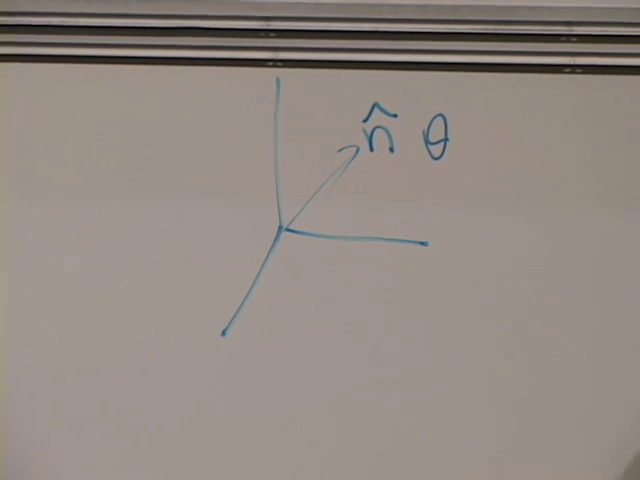
\includegraphics[width=0.58\textwidth]{lecture_03_figure_02.png}\caption{Eine Achse \(\hat{\boldsymbol n}\) und ein Winkel \(\theta\) legen eine räumliche Drehung fest.}\lectureframe{00:02:34}\end{figure}

Eine Richtung auf der Einheitskugel wird durch zwei Parameter festgelegt, etwa Länge und Breite. Der Drehwinkel um diese Richtung liefert einen dritten Parameter. Drehungen bilden daher eine dreiparametrige Familie. Die globalen Identifikationen, die durch Winkel entstehen, die sich um \(2\pi\) unterscheiden, lassen wir zunächst außer Acht; hier ist die lokale Parameterzahl entscheidend.

Die Beschreibung durch Achse und Winkel ist teilweise redundant. Eine Umkehrung der Achse zusammen mit einer Umkehrung des Winkels ergibt dieselbe Operation, und hinreichend große Winkel lassen sich modulo einer vollen Umdrehung reduzieren. Unberührt davon bleibt, dass eine Drehung in der Nähe der Identität durch drei stetig veränderliche Parameter beschrieben wird. Diese lokale Parameterzahl werden wir später mit der Zahl unabhängiger Parameter einer Matrixdarstellung vergleichen.

Die Gruppeneigenschaften lassen sich nun der Reihe nach überprüfen:
\begin{enumerate}\item \emph{Abgeschlossenheit.}Zwei aufeinanderfolgende Drehungen ergeben wieder eine Drehung.
\item \emph{Identität.}Nichts zu tun ist die Identitätsdrehung.
\item \emph{Inverse.}Eine Drehung um \(\theta\) um \(\hat{\boldsymbol n}\) wird durch eine Drehung um \(-\theta\) um dieselbe Achse rückgängig gemacht.
\item \emph{Assoziativität.}Für drei aufeinanderfolgende Drehungen gilt
\[
(R_1R_2)R_3=R_1(R_2R_3).
\]\end{enumerate}

Drehungen sind nicht kommutativ. Eine Drehung um die \(x\)-Achse, gefolgt von einer Drehung um die \(y\)-Achse, führt im Allgemeinen zu einer anderen Orientierung als dieselben beiden Operationen in umgekehrter Reihenfolge:
\begin{equation}
R_x(\alpha)R_y(\beta)\ne R_y(\beta)R_x(\alpha).
\end{equation}
Bei sehr kleinen Winkeln ist die Differenz von zweiter Ordnung. Deshalb können infinitesimale Drehungen beinahe kommutativ erscheinen. Die vollständige Gruppe ist dennoch nichtabelsch.

Die Nichtkommutativität lässt sich auch ohne Gleichungen überprüfen. Nehmen Sie ein Buch oder eine Schachtel und markieren Sie eine Seite als Vorderseite. Drehen Sie das Objekt zuerst um neunzig Grad um die \(x\)-Achse und dann um neunzig Grad um die \(y\)-Achse. Bringen Sie es wieder in die Ausgangsorientierung und vertauschen Sie die Reihenfolge. Die markierte Seite zeigt anschließend in eine andere Richtung. Bei kleinen Winkeln ist der Unterschied schwerer zu erkennen, aber er verschwindet nicht; er setzt bei dem Produkt der beiden kleinen Winkel ein.

\begin{classroomqa}\audiencequestion{Sind diese Drehungen nacheinander und nicht gleichzeitig ausgeführt?\lecturetimestamp{00:04:45}}\lecturerresponse{Ja. Die Gruppenmultiplikation bedeutet, dass eine Operation auf eine andere folgt. Gerade die Reihenfolge dieser aufeinanderfolgenden Drehungen kann die Kommutativität verletzen.}\end{classroomqa}

Dies ist unsere erste nichtabelsche Gruppe. Die spätere Anwendung betrifft nicht die Farbe eines gewöhnlichen Objekts, sondern die roten, grünen und blauen Farbzustände eines Quarks. Es handelt sich um ein internes System mit drei Zuständen, dessen interessante Transformationen die drei Farben miteinander mischen. Gewöhnliche Drehungen liefern ein anschauliches Beispiel dafür, wie eine kontinuierliche Gruppe durch Matrizen wirkt.

Eine Gruppe für sich genommen ist abstrakt. Um sie in der Physik zu verwenden, müssen wir angeben, auf welche Objekte sie wirkt. Eine {Darstellung} ordnet jedem Gruppenelement einen Operator oder eine Matrix zu, sodass die Multiplikation der Gruppenelemente durch die Multiplikation der zugeordneten Matrizen wiedergegeben wird. Verschiedene physikalische Objekte können unterschiedliche Darstellungen derselben Gruppe tragen. Vektoren, Spin-eins-Zustände und Spin-einhalb-Zustände liefern drei Beispiele.

\section{Die dreidimensionale Vektordarstellung}

Ein gewöhnlicher Vektor habe die Komponenten
\begin{equation}
\boldsymbol V=(V_x,V_y,V_z),\qquad V_i,\quad i=1,2,3.
\end{equation}
Man kann den physikalischen Vektor drehen und die Achsen festhalten oder die Koordinatenachsen drehen und den Vektor festhalten. Die Konventionen unterscheiden sich, doch in beiden Beschreibungen werden die Komponenten durch eine \(3\times3\)-Matrix gemischt. Für jedes Paar aus Achse und Winkel \((\hat{\boldsymbol n},\theta)\) schreiben wir
\begin{equation}
V_i'=R_{ij}(\hat{\boldsymbol n},\theta)V_j,
\label{eq:l3-vector-rotation}
\end{equation}
wobei über einen wiederholten Index summiert wird.

Der wiederholte Index \(j\) ist ein stummer Index. Gleichung~\eqref{eq:l3-vector-rotation} bedeutet ausgeschrieben
\begin{equation}
V_i'=R_{i1}V_1+R_{i2}V_2+R_{i3}V_3
\end{equation}
für jede Ausgangskomponente \(i\). Der freie Index \(i\) gibt an, welche Komponente berechnet wird; über den wiederholten Index \(j\) wird summiert, und er kann umbenannt werden, ohne die Gleichung zu ändern. Wenn man diese beiden Rollen auseinanderhält, lassen sich die meisten Indexfehler beim Argument zur Längenerhaltung vermeiden.

\begin{figure}[htbp]\centering
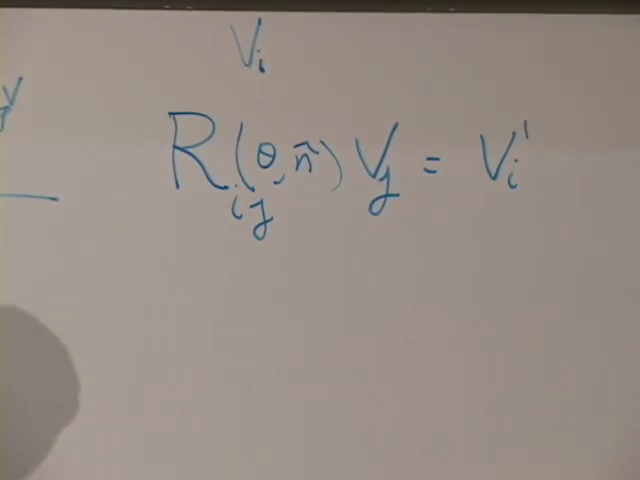
\includegraphics[width=0.68\textwidth]{lecture_03_figure_03.png}\caption{Eine Drehungsmatrix bildet die ursprünglichen Vektorkomponenten auf die gedrehten Komponenten ab.}\lectureframe{00:07:41}\end{figure}

Eine echte Drehung erhält die Länge. Vorerst sind sowohl \(V_i\) als auch \(R_{ij}\) reell, also gilt
\begin{equation}
V_i'V_i'=V_iV_i
\end{equation}
für jeden Vektor. Um die Bedingung an die Matrix sichtbar zu machen, schreiben wir dieselbe Transformation mit verschiedenen stummen Indizes:
\begin{equation}
V_i'=R_{ij}V_j,\qquad V_i'=R_{ik}V_k.
\end{equation}
Multiplikation und Summation über \(i\) ergeben
\begin{align}
V_i'V_i'
 &=R_{ij}V_jR_{ik}V_k\\
 &=R_{ij}R_{ik}V_jV_k.
\end{align}
Dies ist für jede Wahl von \(V\) nur dann gleich \(V_jV_j\), wenn
\begin{equation}
R_{ij}R_{ik}=\delta_{jk}.
\label{eq:l3-orthogonality-index}
\end{equation}
In Matrixschreibweise gilt
\begin{equation}
R^TR=\boldsymbol 1,
\label{eq:l3-orthogonal}
\end{equation}
und damit
\begin{equation}
R^{-1}=R^T.
\end{equation}
Die Transposition vertauscht lediglich Zeilen und Spalten.

Warum muss der Koeffizient \(\delta_{jk}\) sein? Unter der Summation setzt das Kronecker-Delta \(j=k\):
\begin{equation}
\delta_{jk}V_jV_k=V_1^2+V_2^2+V_3^2.
\end{equation}
Wenn \(R_{ij}R_{ik}\) von \(\delta_{jk}\) abwiche, würde sich die Länge in einer bestimmten Richtung oder durch einen bestimmten Kreuzterm \(V_jV_k\) ändern. Da die Gleichheit für jeden möglichen Vektor gelten muss und nicht nur für einen ausgewählten, muss der Matrixkoeffizient selbst der Einheitsmatrix entsprechen.

Gleichung~\eqref{eq:l3-orthogonal} ist die definierende Orthogonalitätsbedingung für diese reelle Matrixdarstellung. Die Matrixmultiplikation bildet die Multiplikationstabelle räumlicher Drehungen nach. Dies ist nicht die einzige Darstellung der Drehgruppe, sondern lediglich die am leichtesten zu veranschaulichende.

Die inverse Beziehung hat eine unmittelbare geometrische Bedeutung. Eine Drehung lässt sich rückgängig machen, ohne eine neue Matrixgleichung zu lösen: Man vertauscht Zeilen und Spalten. Wenn \(R_1\) und \(R_2\) zwei Drehungen darstellen, beschreibt \(R_2R_1\) ihre aufeinanderfolgende Wirkung und ist wiederum orthogonal. Die Matrixoperationen bewahren somit dieselben Eigenschaften Abgeschlossenheit, Identität, Inverses und Assoziativität, die wir geometrisch hergeleitet haben.

\section{Spin eins und die Vektordarstellung}

Die dreidimensionale Darstellung wirkt auch auf Quantenzustände. Ein Spin-eins-Teilchen hat drei mögliche Spinprojektionen:
\begin{equation}
m=+1,\quad 0,\quad -1.
\end{equation}
Sein Spinzustand ist daher eine dreikomponentige Spalte mit Wahrscheinlichkeitsamplituden. Wird das Teilchen gedreht oder die Orientierung eines Magnetfelds verändert, das die Spinachse festlegt, werden diese drei Amplituden durch eine dreidimensionale Darstellung der Drehgruppe miteinander gemischt.

Die Zahl der Spinzustände folgt der bekannten Regel \(2s+1\). Spin null hat einen Zustand, Spin einhalb zwei, Spin eins drei und Spin dreieinhalb vier. Die Dimension des Zustandsvektors hängt also vom Spin ab. Dieselbe physikalische Drehung muss durch Matrizen unterschiedlicher Größe dargestellt werden, wenn sie auf diese verschiedenen Zustandsräume wirkt.

Für ein Spin-eins-Teilchen wählen wir die Basis
\begin{equation}
\lvert 1,+1\rangle,qquad
\lvert 1,0\rangle,qquad
\lvert 1,-1\rangle.
\end{equation}
Ein Zustand ist
\begin{equation}
\lvert\psi\rangle
=c_{+}\lvert1,+1\rangle+c_0\lvert1,0\rangle+c_{-}\lvert1,-1\rangle.
\end{equation}
Durch eine Drehung des Versuchsaufbaus entsteht kein vierter Spinzustand; sie mischt lediglich die drei Koeffizienten \(c_+,c_0,c_-\) miteinander. Der zugehörige Drehoperator muss daher eine \(3\times3\)-Matrix sein.

Für Spin eins transformiert diese Darstellung wie ein gewöhnlicher räumlicher Vektor. Genau das bedeutet es, ein Spin-eins-Teilchen als \emph{Vektorteilchen} zu bezeichnen: Seine drei Spinamplituden und die drei Komponenten eines Vektors gehorchen demselben Drehungsgesetz. Der Quantenzustand muss dabei nicht als wörtlicher Pfeil aufgefasst werden; gemeint ist, wie sich seine Komponenten miteinander mischen.

Diese Entsprechung ist kein Zufall. Ein Dreivektor und ein Spin-eins-Zustand tragen äquivalente dreidimensionale Darstellungen der Drehgruppe. Die Bezeichnung {Vektorteilchen} fasst diese Transformationseigenschaft zusammen. Sie behauptet nicht, dass im Teilchen ein quantenmechanischer Polarisationszustand als winziger starrer Pfeil verborgen ist.

\section{Diskrete und kontinuierliche Symmetrien}

Bevor wir uns Spin einhalb zuwenden, ist es hilfreich, zwei grundlegende Arten von Gruppen zu unterscheiden. Eine Spiegelung ist ein einfaches diskretes Beispiel. Es gibt die Identität und die Spiegelung \(P\); entweder wird gespiegelt oder nicht. Dagegen hängt eine Phase
\begin{equation}
e^{i\phi}
\end{equation}
stetig von \(\phi\) ab, und eine räumliche Drehung hängt stetig von ihrer Achse und ihrem Winkel ab. Solche kontinuierlichen Gruppen nennt man \emph{Lie-Gruppen}, nach Sophus Lie; der Name wird \emph{Li} ausgesprochen. Im Mittelpunkt stehen kontinuierliche Symmetrien, doch auch diskrete Symmetrien bleiben wichtig.

Für die zweielementige Spiegelungsgruppe gilt
\begin{equation}
P^2=1.
\end{equation}
Zwischen \(1\) und \(P\) gibt es keine stetig einstellbare Stärke der Spiegelung. Eine Phasengruppe ist anders: Zwischen \(e^{i\phi_1}\) und \(e^{i\phi_2}\) liegen stetig unendlich viele weitere Phasen. Räumliche Drehungen haben denselben kontinuierlichen Charakter, sind aber anders als \(U(1)\) nichtabelsch.

Spin null liefert die einfachste Darstellung der Drehgruppe. Ein Spin-null-Zustand bleibt unter jeder Drehung unverändert; jedes Gruppenelement wird daher durch die eindimensionale Identität dargestellt:
\begin{equation}
D^{(0)}(R)=1.
\end{equation}
Die Gruppe selbst enthält weiterhin unendlich viele Drehungen; trivial ist lediglich ihre Darstellung auf dem Spin-null-Zustand.

Diese Unterscheidung zwischen einer Gruppe und einer ihrer Darstellungen ist wesentlich. Die Drehgruppe reduziert sich nicht auf eine Gruppe mit nur einem Element, wenn sie auf einen Skalar wirkt. Vielmehr wird jedes ihrer Elemente auf diesem bestimmten Skalarzustand durch dieselbe Zahl \(1\) dargestellt.

\section{Ein allgemeiner Spin-einhalb-Zustand}

Ein Spin-einhalb-System hat zwei Basiszustände. Bezogen auf eine gewählte \(z\)-Achse gilt
\begin{equation}
\lvert\uparrow\rangle=
\begin{pmatrix}1\\0\end{pmatrix},
\qquad
\lvert\downarrow\rangle=
\begin{pmatrix}0\\1\end{pmatrix}.
\end{equation}
Ein allgemeiner Zustand ist ein zweikomponentiger Spinor:
\begin{equation}
\lvert\psi\rangle=
\begin{pmatrix}\alpha_1\\\alpha_2\end{pmatrix},
\qquad
|\alpha_1|^2+|\alpha_2|^2=1.
\label{eq:l3-spinor}
\end{equation}
Die Einträge sind komplex. Für \((\alpha_1,\alpha_2)=(1,0)\) ist der Spin nach oben gerichtet, für \((0,1)\) nach unten. Eine allgemeine normierte Linearkombination beschreibt einen Spin, der entlang einer anderen Richtung polarisiert ist.

Die Begriffe {auf} und {ab} haben erst dann eine Bedeutung, wenn eine Achse gewählt wurde. Hier ist dies \(z\). Eine andere Messachse hat ein anderes Paar von Basiszuständen, und ein Zustand mit eindeutigem Spin nach oben entlang einer Achse erscheint in einer anderen Basis im Allgemeinen als Überlagerung. Eine Drehung des physikalischen Spins oder der Bezugsachsen ändert die Koeffizienten entsprechend.

Zwei komplexe Amplituden enthalten vier reelle Parameter. Durch die Normierung fällt einer weg; ein weiterer entfällt, weil die globale Phase physikalisch irrelevant ist. Es bleiben zwei reelle Parameter. Genau so viele werden benötigt, um eine Richtung auf einer Kugel festzulegen. Um Drehungen zu untersuchen, müssen wir die explizite Abbildung zwischen \((\alpha_1,\alpha_2)\) und dieser Richtung nicht herleiten.

Die globale Phase wird herausdividiert, weil
\begin{equation}
\begin{pmatrix}\alpha_1\\\alpha_2\end{pmatrix}
\quad\hbox{and}\quad
e^{i\chi}
\begin{pmatrix}\alpha_1\\\alpha_2\end{pmatrix}
\end{equation}
denselben physikalischen Strahl darstellen. Die Normierung legt die Gesamtwahrscheinlichkeit fest, nicht eine Richtung im gewöhnlichen euklidischen Raum. Nach beiden Identifikationen lassen sich die verbleibenden zwei Parameter als Polar- und Azimutwinkel der Spinpolarisationsrichtung auffassen.

Bei einer Drehung des Spins wird sein Zustand zu
\begin{equation}
\alpha_i'=U_{ij}\alpha_j,
\qquad
\begin{pmatrix}\alpha_1'\\\alpha_2'\end{pmatrix}
=
\begin{pmatrix}
U_{11}&U_{12}\\
U_{21}&U_{22}
\end{pmatrix}
\begin{pmatrix}\alpha_1\\\alpha_2\end{pmatrix}.
\label{eq:l3-spinor-transform}
\end{equation}
Räumliche Drehungen besitzen also eine zweidimensionale Matrizendarstellung, die auf Spinoren wirkt. Diese Darstellung weist eine globale Zweideutigkeit auf, auf die wir später zurückkommen; lokal haben die Matrizen die Transformationseigenschaften, die wir im Folgenden benötigen.

Das transformierte Paar \((\alpha_1',\alpha_2')\) muss wiederum einen möglichen Quantenzustand ergeben. Die erste Frage zu \(U\) betrifft daher nicht die explizite Formel für Achse und Winkel, sondern die Bedingung, dass die Normierung jedes Eingangsspinors erhalten bleibt.

\section{Wahrscheinlichkeitserhaltung und unitäre Matrizen}

Eine Drehung muss einen normierten Zustand auf einen anderen normierten Zustand abbilden:
\begin{equation}
\alpha_i^*\alpha_i=\alpha_i'^*\alpha_i'=1.
\end{equation}
Einsetzen von Gleichung~\eqref{eq:l3-spinor-transform} ergibt
\begin{align}
\alpha_i'^*\alpha_i'
 &=(U_{ij}\alpha_j)^*(U_{ik}\alpha_k)\\
 &=\alpha_j^*U_{ij}^*U_{ik}\alpha_k.
\end{align}
Das Analogon zur Bedingung für reelle Vektoren lautet daher
\begin{equation}
(U^T)^*U=\boldsymbol 1.
\end{equation}
Die Transposition zusammen mit komplexer Konjugation ist die hermitesche Konjugation:
\begin{equation}
U^\dagger=(U^T)^*,
\end{equation}
Somit lautet die Bedingung für den Erhalt der Normierung
\begin{equation}
U^\dagger U=\boldsymbol 1.
\label{eq:l3-unitarity}
\end{equation}

Die zusätzliche komplexe Konjugation ist die einzige wesentliche Änderung gegenüber der Rechnung mit reellen Vektoren. Für einen reellen Vektor ist \(V_iV_i\) eine Länge. Für einen Spinor ist \(\alpha_i^*\alpha_i\) eine Wahrscheinlichkeit. Komplexe Konjugation ist nötig, damit diese Wahrscheinlichkeit reell und nichtnegativ ist; deshalb tritt an die Stelle der Transposition die hermitesche Konjugation.

Gleichung~\eqref{eq:l3-unitarity} liefert unmittelbar auch die inverse Matrix:
\begin{equation}
U^{-1}=U^\dagger.
\end{equation}
Die inverse Drehung erhält also dieselbe Wahrscheinlichkeitsnorm. Wie bei gewöhnlichen Drehmatrizen bleibt auch ein Produkt unitärer Matrizen unitär, sodass die Darstellung die Gruppenmultiplikation respektiert.

\begin{figure}[htbp]\centering
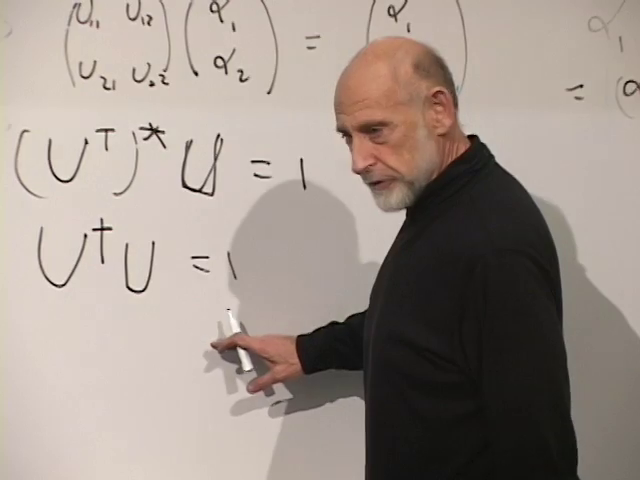
\includegraphics[width=0.62\textwidth]{lecture_03_figure_04.png}\caption{Die Spinordrehungsmatrix erfüllt \(U^\dagger U=\boldsymbol 1\).}\lectureframe{00:27:41}\end{figure}

Matrizen, die Gleichung ~\eqref{eq:l3-unitarity} erfüllen, sind unitär. Eine allgemeine komplexe \(2\times2\)-Matrix wird durch acht reelle Parameter beschrieben. Die Unitarität ist eine Matrixgleichung für \(2\times2\)-Matrizen, die vier unabhängige reelle Bedingungen liefert; damit bleiben vier Parameter. Eine räumliche Drehung hat nur drei. Eine weitere Einschränkung ist nötig, um die Spinordarstellung der Drehungen aus der Gesamtheit von \(U(2)\) herauszuheben.

Die vier Bedingungen lassen sich auch verstehen, indem man die beiden Spalten von \(U\) als zwei komplexe Vektoren auffasst. Jede Spalte muss die Norm eins haben, was zwei reelle Bedingungen ergibt. Außerdem müssen die Spalten orthogonal sein, was einer komplexen oder zwei reellen Bedingungen entspricht. Insgesamt sind es also vier. Wie sich herausstellen wird, ist der verbleibende vierte Parameter in \(U(2)\) eine globale Determinantenphase und keine neue räumliche Drehung.

\section{Determinante eins und \texorpdfstring{\(SU(2)\)}{SU(2)}}

Die zusätzliche Bedingung lautet
\begin{equation}
\det U=1.
\label{eq:l3-det-one}
\end{equation}
Sie ist mit der Gruppenmultiplikation verträglich, denn
\begin{equation}
\det(AB)=\det A\,\det B.
\end{equation}
Das Produkt zweier unitärer Matrizen mit Determinante eins hat wiederum Determinante eins, und auch die Identität hat Determinante eins. Diese Matrizen bilden eine abgeschlossene Untergruppe.

Auch die Inverse gehört zu dieser Untergruppe. Wenn \(\det U=1\), dann gilt
\begin{equation}
\det U^{-1}=\frac{1}{\det U}=1.
\end{equation}
Die Bedingung Determinante eins entfernt also weder die Identität noch stört sie die Abgeschlossenheit oder führt zum Verlust der Inversen. Sie legt konsistent eine Gruppe mit einem kontinuierlichen Parameter weniger fest.

Aus der Unitarität folgt allein
\begin{equation}
\det(U^\dagger U)=
(\det U)^*\det U
=|\det U|^2=1.
\end{equation}
Sie erzwingt nicht, dass \(\det U\) gleich \(+1\) oder \(-1\) ist. Die Determinante einer allgemeinen unitären Matrix kann eine beliebige Phase sein:
\begin{equation}
\det U=e^{i\phi},
\qquad
\det U^\dagger=e^{-i\phi}.
\end{equation}
Bedingung~\eqref{eq:l3-det-one} legt diese ansonsten freie Phase fest und entfernt einen reellen Parameter.

\begin{classroomqa}\audiencequestion{Erzwingt \(U^\dagger U=\boldsymbol 1\) ohne die Bedingung Determinante eins, dass \(\det U^\dagger\) gleich \(\det U\) oder nur \(+1\) oder \(-1\) ist?\lecturetimestamp{00:31:21}}\lecturerresponse{Nein. Die beiden Determinanten sind komplex konjugiert. Sie können \(e^{i\phi}\) und \(e^{-i\phi}\) sein; ihr Produkt ist dann eins. Die Einschränkung auf die spezielle unitäre Gruppe legt anschließend beide auf eins fest.}\end{classroomqa}

Die unitären \(n\times n\)-Matrizen bilden \(U(n)\). Für \(n=1\) ist eine unitäre Matrix einfach die Phase \(e^{i\phi}\); somit ergibt sich \(U(1)\). Die Untergruppe mit Determinante eins heißt \emph{spezielle unitäre Gruppe}:
\begin{equation}
SU(n)=\{U\in U(n):\det U=1\}.
\end{equation}
Auf den zweikomponentigen Spinor wirkt \(SU(2)\), eine dreiparametrige Gruppe.

Die Bezeichnung hält beide Einschränkungen fest: \(U\) steht für unitär, während \(S\) speziell bedeutet, also Determinante eins. Diese speziellen unitären Gruppen treten immer wieder auf, weil sie ein komplexes Skalarprodukt erhalten und zugleich die unabhängige globale Phase der Determinante ausschließen.

Lokal hat \(SU(2)\) dieselbe Drehungsalgebra und Multiplikationsstruktur, die für Drehungen von Spin-einhalb-Zuständen nötig sind. Global muss man die zuvor zurückgestellte Feinheit berücksichtigen: \(SU(2)\) ist die zweifache Überlagerung der gewöhnlichen Drehgruppe \(SO(3)\), sodass jeweils zwei Elemente von \(SU(2)\) einer räumlichen Drehung entsprechen. \editorialnote{Die Formulierung mit der zweifachen Überlagerung präzisiert die im Ausgangstext erwähnte, aber nicht ausgeführte Zweideutigkeit.}

\section{Infinitesimale Drehungen und Pauli-Matrizen}

\begin{classroomqa}\audiencequestion{Wie kommen die Spinmatrizen oder Pauli-Matrizen in diese Konstruktion?\lecturetimestamp{00:33:16}}\lecturerresponse{Sie treten auf, wenn man ein Gruppenelement betrachtet, das sehr nahe an der Identität liegt und einer Drehung um einen sehr kleinen Winkel entspricht. Sie sind die Erzeugenden dieser infinitesimalen Drehungen.}\end{classroomqa}

Wir beginnen mit
\begin{equation}
U=\boldsymbol 1+\epsilon M+O(\epsilon^2),
\label{eq:l3-small-u-anti}
\end{equation}
wobei \(\epsilon\) reell und klein ist. Dann gilt
\begin{equation}
U^\dagger=\boldsymbol 1+\epsilon M^\dagger+O(\epsilon^2),
\end{equation}
und aus der Unitarität folgt
\begin{align}
U^\dagger U
 &=\boldsymbol 1+\epsilon(M^\dagger+M)+O(\epsilon^2).
\end{align}
In erster Ordnung erhalten wir
\begin{equation}
M^\dagger=-M.
\end{equation}
Die Matrix \(M\) in Gleichung~\eqref{eq:l3-small-u-anti} ist also antihermitesch.

Es werden nur Terme linear in \(\epsilon\) beibehalten. Das Produkt \(\epsilon^2M^\dagger M\) wird vernachlässigt, weil es von zweiter Ordnung ist. Darin liegt der Vorteil, nahe an der Identität zu arbeiten: Nichtlineare Gruppenbedingungen werden zu linearen Bedingungen an ihre Erzeugenden.

Praktischer ist es, den Faktor \(i\) auszuklammern:
\begin{equation}
U=\boldsymbol 1+i\epsilon H+O(\epsilon^2).
\label{eq:l3-small-u-herm}
\end{equation}
Durch komplexe Konjugation wird \(i\) zu \(-i\), also gilt
\begin{equation}
U^\dagger=\boldsymbol 1-i\epsilon H^\dagger+O(\epsilon^2).
\end{equation}
Nun ist
\begin{equation}
U^\dagger U
=\boldsymbol 1+i\epsilon(H-H^\dagger)+O(\epsilon^2),
\end{equation}
und die Unitarität in erster Ordnung verlangt
\begin{equation}
H^\dagger=H.
\end{equation}
Wenn der Faktor \(i\) ausgeklammert ist, ist die Erzeugende hermitesch.

Die Multiplikation mit \(i\) ändert nicht, welche infinitesimalen Matrizen zulässig sind; sie ändert lediglich die Konvention zur Benennung der Erzeugenden. In der Physik wählt man gewöhnlich hermitesche Erzeugende, weil ihre Eigenwerte reell sind und die zugehörigen Observablen wie der Drehimpuls hermitesch sind.

Die Bedingung Determinante eins erzwingt Spurfreiheit\editorialnote{Bei der mündlichen Entwicklung der Determinante werden die Indizes kurzzeitig falsch wiedergegeben. Der korrigierte lineare Term lautet \(A_{11}+A_{22}=\operatorname{tr}A\); Produkte der Nichtdiagonalelemente beginnen erst in quadratischer Ordnung.}. Für eine kleine \(2\times2\)-Matrix \(A\) gilt
\begin{equation}
\det(\boldsymbol 1+A)
=
\det
\begin{pmatrix}
1+A_{11}&A_{12}\\
A_{21}&1+A_{22}
\end{pmatrix}.
\end{equation}
Entwickelt man die Determinante, erhält man
\begin{align}
\det(\boldsymbol 1+A)
 &=(1+A_{11})(1+A_{22})-A_{12}A_{21}\\
 &=1+A_{11}+A_{22}+O(A^2)\\
 &=1+\operatorname{tr}A+O(A^2).
\end{align}
Wenden wir dies auf \(A=i\epsilon H\) an, folgt
\begin{equation}
\det U=1+i\epsilon\,\operatorname{tr}H+O(\epsilon^2).
\end{equation}
Daher verlangt \(\det U=1\)
dass
\begin{equation}
\operatorname{tr}H=0.
\end{equation}
Die Spurbedingung entfernt genau die zur Einheitsmatrix proportionale Erzeugende. Eine allgemeine hermitesche \(2\times2\)-Matrix hat vier reelle Parameter: zwei reelle Diagonaleinträge und einen komplexen Nebendiagonaleintrag. Ihre Spur legt eine reelle Kombination fest, sodass drei Parameter übrig bleiben. Das entspricht den drei Achsen, um die eine infinitesimale räumliche Drehung erfolgen kann.

Die infinitesimalen Erzeugenden von \(SU(2)\) sind somit spurfrei-hermitesche \(2\times2\)-Matrizen. Die drei Pauli-Matrizen bilden eine Basis:
\begin{equation}
\begin{aligned}
\sigma_x&=
\begin{pmatrix}0&1\\1&0\end{pmatrix},
&
\sigma_y&=
\begin{pmatrix}0&-i\\i&0\end{pmatrix},
\\[0.4em]
\sigma_z&=
\begin{pmatrix}1&0\\0&-1\end{pmatrix}.
\end{aligned}
\end{equation}
Jede Erzeugende lässt sich schreiben als
\begin{equation}
H=a_x\sigma_x+a_y\sigma_y+a_z\sigma_z.
\end{equation}
Eine kleine Drehung um die \(x\)-Achse wählt \(\sigma_x\) aus, eine um die \(y\)-Achse \(\sigma_y\), und eine Drehung um eine beliebige andere Achse wählt die entsprechende Linearkombination aus. In Einheiten mit \(\hbar=1\) lauten die Spinoperatoren
\begin{equation}
S_i=\frac{\sigma_i}{2}.
\end{equation}

Eine Achse, die beispielsweise genau zwischen \(x\) und \(y\) liegt, verwendet eine Erzeugende proportional zu
\begin{equation}
\frac{\sigma_x+\sigma_y}{\sqrt2}.
\end{equation}
Die Richtung des Koeffizientenvektors \((a_x,a_y,a_z)\) legt die Drehachse fest, während sein Betrag zusammen mit \(\epsilon\) den kleinen Winkel bestimmt. So hängen die aus den Drehimpulskommutatoren bekannten Spinmatrizen mit endlichen Drehoperatoren zusammen. Insbesondere kodieren
\begin{equation}
[S_x,S_y]=iS_z
\end{equation}
und die zyklisch vertauschten Beziehungen die bereits geometrisch erkannte Nichtkommutativität. Die übliche Formel für eine endliche Drehung erhält man, indem man die infinitesimale Erzeugende exponentiert\editorialnote{Die Exponentialformel für endliche Drehungen ist die übliche Fortsetzung der infinitesimalen Konstruktion; die Quelle leitet nur die Bedingungen an die Erzeugenden und ihre Pauli-Matrix-Basis her.}:
\begin{equation}
U(\hat{\boldsymbol n},\theta)
=\exp\left(-\frac{i\theta}{2}\,
\hat{\boldsymbol n}\cdot\boldsymbol\sigma\right).
\end{equation}\section{Ein dreidimensionaler Farbraum}

Die Kombination von Darstellungen kann warten. Wir verlassen nun den räumlichen Spin und wenden uns wieder der Quarkfarbe zu. Ein Quark hat weiterhin Spin einhalb, doch seine Farbe ist ein davon unabhängiger Freiheitsgrad mit drei Zuständen:
\begin{equation}
\lvert r\rangle,\qquad
\lvert g\rangle,\qquad
\lvert b\rangle.
\end{equation}
Ein allgemeiner Farbenzustand ist
\begin{equation}
\begin{aligned}
\lvert q\rangle_{\mathrm{color}}
={}&
\alpha_r\lvert r\rangle
+\alpha_g\lvert g\rangle
+\alpha_b\lvert b\rangle,
\\
&|\alpha_r|^2+|\alpha_g|^2+|\alpha_b|^2=1.
\end{aligned}
\end{equation}
Äquivalent dazu gilt
\begin{equation}
q=
\begin{pmatrix}
\alpha_r\\
\alpha_g\\
\alpha_b
\end{pmatrix}.
\end{equation}
Die Betragsquadrate sind die Wahrscheinlichkeiten für Rot, Grün und Blau in einer gewählten Farbbasis. Dieselbe Tripletnotation kann auch drei Quarkfeldoperatoren zu einer Spalte zusammenfassen:
\begin{equation}
\psi=
\begin{pmatrix}
\psi_r\\
\psi_g\\
\psi_b
\end{pmatrix}.
\end{equation}

Spin und Farbe müssen gedanklich getrennt bleiben. Der Spinindex gibt an, wie der Zustand unter Drehungen des physikalischen Raums transformiert. Der Farbindex gibt an, wie er sich unter einer internen Symmetrie transformiert, die das Labor nicht dreht. Ein Quarkzustand trägt beide Indizes, obwohl wir den Spin in der vorliegenden Diskussion ausblenden, um uns auf die Farbe zu konzentrieren.

Drei Feldoperatoren in eine Spalte zu schreiben, ist mehr als bloße Buchführung. So lässt sich die Symmetrie mit einer einzigen Matrixgleichung formulieren. Eine Transformation kann ein rotes Feld in eine Linearkombination roter, grüner und blauer Felder überführen, so wie eine räumliche Drehung eine Vektorkomponente in eine Linearkombination der anderen Komponenten überführt.

Zunächst kann man sich diskrete Transformationen vorstellen, die zwei Farben vertauschen. Die größere Symmetrie umfasst kontinuierliche Mischungen aller drei Farben. Bei einer einfachen Vertauschungsmatrix ist möglicherweise eine zusätzliche Phase nötig, damit ihre Determinante eins ist; mit dieser Phase ist die Vertauschung in die spezielle unitäre Gruppe eingebettet.

Für zwei Basiszustände wird die unveränderte Vertauschung dargestellt durch
\begin{equation}
X=
\begin{pmatrix}0&1\\1&0\end{pmatrix},
\qquad
\det X=-1.
\end{equation}
Multipliziert man die gesamte Matrix mit \(i\), erhält man
\begin{equation}
\det(iX)=i^2\det X=1.
\end{equation}
Mit einer passend gewählten Phase kann die diskrete Vertauschung somit als bestimmtes Element der größeren kontinuierlichen Gruppe auftreten.

\begin{classroomqa}\audiencequestion{Hat eine Matrix, die lediglich zwei Basiszustände vertauscht, für \(SU(2)\) die falsche Determinante?\lecturetimestamp{00:43:46}}\lecturerresponse{Die unveränderte Vertauschung hat die Determinante \(-1\). Ein geeigneter Faktor \(i\) liefert eine Darstellung mit Determinante eins, sodass sich die Vertauschung in die kontinuierlichen speziellen unitären Transformationen einordnen lässt.}\end{classroomqa}

\section{\texorpdfstring{\(SU(3)\)}{SU(3)} und die acht Farberzeugenden}

Die kontinuierliche Farbtransformation lautet
\begin{equation}
\begin{aligned}
q'&=Uq,
&
U^\dagger U&=\boldsymbol 1,
\\
\det U&=1,
&
U&\in SU(3).
\end{aligned}
\label{eq:l3-su3-action}
\end{equation}
Mathematisch ist dies dieselbe spezielle unitäre Konstruktion wie bei den Spinoren, doch nun ist \(U\) eine \(3\times3\)-Matrix. Es handelt sich nicht um eine Drehung des physikalischen Raums, sondern um eine Drehung im internen Farbraum.

Die Unitarität erhält die Normierung des Farbenzustands:
\begin{equation}
q^\dagger q
=|\alpha_r|^2+|\alpha_g|^2+|\alpha_b|^2.
\end{equation}
Die Bedingung Determinante eins entfernt die Richtung der gemeinsamen Phase \(U(1)\) aus der kontinuierlichen Mischung. Die resultierenden Matrizen können einfache Vertauschungen, relative Phasenänderungen und echte kontinuierliche Überlagerungen bewirken und bleiben dabei Elemente einer einzigen abgeschlossenen Gruppe.

Die Parameterzahl ergibt sich unmittelbar. Eine komplexe \(3\times3\)-Matrix hat neun komplexe Einträge, also achtzehn reelle Parameter. Die Matrixgleichung \(U^\dagger U=\boldsymbol 1\) liefert neun reelle Bedingungen. Die Determinante eins entfernt einen weiteren Parameter:
\begin{equation}
\dim SU(3)=18-9-1=8.
\end{equation}
Damit hat \(SU(3)\) acht unabhängige infinitesimale Erzeugende.

Die neun reellen Unitaritätsbedingungen lassen sich wiederum anhand der Spalten von \(U\) verstehen. Jede der drei komplexen Spalten muss die Norm eins haben, und jedes Spaltenpaar muss orthogonal sein. Diese Bedingungen entfernen neun der ursprünglich achtzehn reellen Parameter. Die Determinantenphase entfernt den zehnten; acht bleiben übrig. Dies ist das Analogon für drei Zustände zur Zählung \(8-4-1=3\) für \(SU(2)\).

Das Auftreten der Acht ist derselbe Sachverhalt, aus dem letztlich auch die acht Gluonenarten hervorgehen. Die Aussage, es gebe keine neun Gluonen, weil die Determinantenbedingung eine Richtung entfernt habe, ist lediglich eine Gedächtnisstütze. Genauer zerfallen die neun Farb-Antifarb-Matrizen in eine farbsinguläre Richtung, die proportional zur Einheitsmatrix ist, und acht spurfreie Richtungen. Die acht spurfreien Generatoren bilden die adjungierte Farbstruktur, die von den Gluonen der QCD getragen wird.\editorialnote{Die Formulierung als Singulett plus Oktett ist die standardmäßige präzise Fassung der bewusst heuristischen Determinantenbemerkung in der Quelle; die Konstruktion des Eichfeldes wird später behandelt.}

An dieser Stelle ist der Zusammenhang mit den acht Gluonen ein Hinweis, noch keine vollständige Herleitung. Um Eichbosonen zu erhalten, muss man die Farbsymmetrie zu einer lokalen Symmetrie machen und die kompensierenden Felder bestimmen. Die Parameterzählung hat bereits gezeigt, dass es acht unabhängige Richtungen gibt, in denen eine \(SU(3)\)-Farbtransformation von der Identität abweichen kann.

\section{Die Farbsymmetrie schränkt die QCD ein}

Die grundlegende Aussage über die Symmetrie lautet, dass die Physik unter der Farbtransformation in Gleichung~\eqref{eq:l3-su3-action} invariant ist. Dies ist die zentrale innere Symmetrie der Quantenchromodynamik. Die Mischung der Farbkomponenten ist formal analog zur Mischung von Spin-up- und Spin-down-Amplituden; diese Spinortransformationen wiederum stehen in Beziehung zu Drehungen räumlicher Richtungen. Die drei Räume dürfen jedoch nicht miteinander verwechselt werden.

Farbe als Symmetrie zu bezeichnen bedeutet, dass eine Änderung der Farbbasis die physikalischen Vorhersagen nicht verändert. Rot, Grün und Blau sind zweckmäßige Bezeichnungen für drei Basisvektoren, keine beobachtbaren Pigmente. Eine gleichzeitige \(SU(3)\)-Drehung der Farbkomponenten muss die Form der Gesetze unverändert lassen. Diese Invarianz ist kein optionales ästhetisches Merkmal, sondern das Ordnungsprinzip der QCD.

Die Symmetrie schränkt die Lagrange-Dichte ein. Im früheren \(U(1)\)-Beispiel führte die Invarianz unter einer gemeinsamen Phasentransformation dazu, dass zulässige Terme gleich viele Faktoren eines Feldes und seines konjugierten Feldes enthalten mussten. In der QCD muss ebenso jeder Term unter der \(SU(3)\)-Farbtransformation invariant sein. Diese Forderung hat Folgen für die Wechselwirkungen, die Erhaltungsgrößen und die Form des Gluonenfeldes.

Nehmen wir an, ein vorgeschlagener Term trage einen freien Farbindex. Unter Gleichung~\eqref{eq:l3-su3-action} wird dieser Index gedreht; der Term kann daher für sich genommen nicht invariant sein. Zulässige Terme müssen Farbindizes zu invarianten Kombinationen kontrahieren oder Eichfelder verwenden, deren Transformation die Änderung kompensiert. Darin zeigt sich die praktische Wirkung des Symmetrieprinzips: Es schließt beliebige Kopplungen aus und ordnet die verbleibenden Wechselwirkungen.

Die vollständige Konstruktion der QCD erfordert noch einen weiteren Schritt: Die Farbtransformation muss von Punkt zu Punkt variieren dürfen, und das Eichfeld muss diese lokale Änderung kompensieren.\editorialnote{Die Lokalisierung der Farbsymmetrie ist die standardmäßige eichfeldtheoretische Vervollständigung der globalen \(SU(3)\)-Symmetrie; in dieser Vorlesung wird sie nicht ausgeführt.}Diese Ausarbeitung gehört zum nächsten Schritt. Für den Moment steht die wesentliche Struktur fest: ein Farbtriplett, auf das eine spezielle unitäre Symmetrie eines dreidimensionalen Zustandsraums mit acht Generatoren wirkt.

Die gruppentheoretische Rechnung ist für den Moment weit genug geführt. Wir begannen mit Drehungen, die sich im gewöhnlichen Raum veranschaulichen lassen, gingen zu den Matrizen über, die auf Vektoren und Spinoren wirken, und übertrugen dieselbe Argumentation anschließend auf einen inneren Farbraum. Als Nächstes können wir zur Teilchenphysik zurückkehren und dabei auf den bereits verfügbaren mathematischen Rahmen zurückgreifen, statt dem Formalismus die gesamte physikalische Darstellung auf einmal aufzubürden.
\chapter{Farbdarstellungen, Hadronen und Confinement}

\paragraph{Ein kurzes einleitendes Zwischenspiel.}
Bevor wir zur Gruppentheorie zurückkehren, sei ein unverhohlenes Eigenlob erlaubt. \emph{Der Krieg um das Schwarze Loch} erzählt von der langjährigen Auseinandersetzung mit Stephen Hawking darüber, ob Schwarze Löcher Quanteninformation zerstören. Das Buch hält auch eine Grausamkeit fest, die theoretischen Physikern eigentümlich ist: nicht nur Schrödingers Katze, sondern auch Susskinds Fisch und seinen unglücklichen Weg hinunter in die Toilette. Damit wäre diese Pflicht erfüllt; kehren wir zu Alice und Bob zurück. Alice leidet noch immer, denn Bob lässt sie weiterhin Gruppentheorie lernen.

\lectureoverview{Eine Symmetrie wird durch ihre Wirkung auf Zustände physikalisch. Wir beginnen mit Rotationen, um Darstellungen und Erzeugende einzuführen, und wiederholen die Konstruktion anschließend für Farbe \(SU(3)\). Farbdarstellungen setzen sich zu Hadronen zusammen, und ihre Dynamik erklärt, warum isolierte Farbe niemals beobachtet wird.}

\section{Die Gruppe und die Objekte, auf die sie wirkt}

In jeder Diskussion über Symmetrien gibt es zwei Grundgedanken. Erstens eine abstrakte Gruppe: eine Menge von Operationen mit einem Multiplikationsgesetz, einem Einselement und inversen Elementen. Zweitens die Objekte, auf die diese Operationen wirken. Die beiden Gedanken lassen sich unterscheiden, in der Physik aber nicht voneinander trennen. Eine Symmetrie ist relevant, weil sie physikalische Zustände, Felder, Koordinaten oder Observablen transformiert.

\begin{classroomqa}
\audiencequestion{Eine Gruppe wurde sowohl als abstrakte Multiplikationstafel als auch als Matrizen beschrieben, die auf physikalische Objekte wirken. Lassen sich diese beiden Aspekte voneinander trennen?
\lecturetimestamp{00:01:58}}
\lecturerresponse{Es handelt sich um verschiedene Beschreibungsebenen, die jedoch vollständig miteinander verknüpft sind. Eine Rotation existiert als abstrakte Operation, bevor wir festlegen, worauf sie wirkt. Die Physik fragt dann, wie dieselbe Operation auf die für ein bestimmtes System relevanten Zustände und Größen wirkt. Die Matrizen geben diese konkrete Wirkung an und bewahren dabei das abstrakte Multiplikationsgesetz.}
\end{classroomqa}

Räumliche Rotationen sind das anschaulichste Beispiel. Klassisch kann dieselbe Rotation auf die Koordinaten eines Teilchens, auf die Richtung eines Magneten oder auf einen beliebigen anderen Vektor wirken. In der Quantenmechanik liegen Zustände in einem linearen Vektorraum, daher wird eine Rotation durch einen linearen Operator auf diesem Raum dargestellt. Bezeichnet \(g\) ein abstraktes Gruppenelement und \(D(g)\) dessen Matrixdarstellung, so bedeutet Konsistenz
\begin{equation}
D(g_1g_2)=D(g_1)D(g_2),
\qquad
D(e)=\boldsymbol 1.
\end{equation}
Die Matrizen müssen nicht wie die abstrakten Operationen aussehen, aber ihre Multiplikation muss die Gruppenmultiplikation reproduzieren.
\editorialnote{Die Homomorphiegleichung formuliert ausdrücklich die im Text beschriebene Entsprechung zwischen Gruppen- und Matrizenmultiplikation.}

Die Dimension der Matrix wird durch den Zustandsraum bestimmt, nicht allein durch die abstrakte Gruppe. Betrachten wir nur den Spin eines Elektrons, gibt es zwei orthogonale Möglichkeiten: Spin nach oben und Spin nach unten. Ein Zustand ist dann ein Spaltenvektor mit zwei Komponenten. Rotationen wirken daher durch \(2\times2\)-Matrizen. Für zwei Spin-ein-Halb-Objekte gibt es vier Basiszustände,
\begin{equation}
\ket{\uparrow\uparrow},\qquad
\ket{\uparrow\downarrow},\qquad
\ket{\downarrow\uparrow},\qquad
\ket{\downarrow\downarrow},
\end{equation}
und die induzierte Wirkung auf dem kombinierten Raum ist vierdimensional.

Die bekannte Abfolge lautet
\begin{equation}
\begin{array}{c|c|c}
\text{spin} & \text{number of states} & \text{matrix dimension}\\
\hline
0 & 1 & 1\times1\\
\frac12 & 2 & 2\times2\\
1 & 3 & 3\times3\\
\frac32 & 4 & 4\times4
\end{array}
\end{equation}
und so weiter. Ein Spin-null-Zustand bildet die triviale Darstellung: Jede Rotation lässt ihn unverändert. Die einzeilige Matrix ist einfach \(1\). Ein Spin-eins-Zustand hat drei Komponenten, und seine Rotationsmatrizen sind die vertrauten dreidimensionalen Vektorrotationen. Allgemeiner hat Spin \(j\) genau \(2j+1\) Zustände.

Die Darstellung kann auch unendlichdimensional sein. Beschreiben wir die gesamte Bahnbewegung eines Elektrons statt nur seines Spins, enthält ein Zustand eine Amplitude für jede Position oder, gleichwertig, für jeden Impuls. Der Rotationsoperator wirkt dann auf einem unendlichdimensionalen Raum von Wellenfunktionen. Dieselbe abstrakte Rotationsgruppe besitzt also triviale, zweidimensionale, dreidimensionale und unendlichdimensionale Darstellungen. Diese Tatsache werden wir wiederverwenden, wenn wir von Spin zu Farbe übergehen.

\section{Warum Spinrotationen speziell unitär sind}

Betrachten wir wieder den Spin eines einzelnen Elektrons und lassen seine Bahnbewegung außer Acht. Eine Rotation wird durch eine unitäre \(2\times2\)-Matrix \(U\) dargestellt,
\begin{equation}
U^\dagger U=\boldsymbol 1,
\qquad
U^{-1}=U^\dagger.
\label{eq:l4-unitarity}
\end{equation}
Die inverse Transformation muss die Rotation rückgängig machen, und Unitarität erhält die Norm und damit jede Wahrscheinlichkeit.

Eine allgemeine \(2\times2\)-Matrix mit komplexen Einträgen enthält vier komplexe beziehungsweise acht reelle Parameter. Gleichung~\eqref{eq:l4-unitarity} legt vier unabhängige reelle Bedingungen fest, sodass vier Parameter übrig bleiben. Eine gewöhnliche räumliche Rotation hat nur drei: Zwei Parameter bestimmen die Achse, einer den Winkel. Die unitäre Matrix enthält also eine Phase zu viel. Die zusätzliche Bedingung lautet
\begin{equation}
\det U=1.
\label{eq:l4-det-one}
\end{equation}
Die Parameterzahl ist dann
\begin{equation}
8-4-1=3.
\end{equation}

Die Bedingung, dass die Determinante eins ist, bleibt bei Multiplikation erhalten, denn
\begin{equation}
\det(AB)=\det A\,\det B.
\end{equation}
Haben zwei Matrizen jeweils Determinante eins, so gilt das auch für ihr Produkt. Die Bedingung ist außerdem mit der Unitarität vereinbar. Bilden wir die Determinante von Gleichung~\eqref{eq:l4-unitarity}, so folgt
\begin{equation}
1=\det(U^\dagger U)
=\det(U^\dagger)\det U
=(\det U)^*\det U.
\end{equation}
Die Determinante einer unitären Matrix liegt folglich auf dem Einheitskreis:
\begin{equation}
\det U=e^{i\phi}.
\end{equation}

\begin{classroomqa}
\audiencequestion{Muss die Determinante aufgrund der Unitarität reell sein?
\lecturetimestamp{00:12:10}}
\lecturerresponse{Nein. Die Unitarität verlangt lediglich, dass ihr Betrag eins ist. Die Determinante kann eine beliebige reine Phase \(e^{i\phi}\) sein. Bei einer zweidimensionalen Matrix entfernt die Multiplikation von \(U\) mit \(e^{-i\phi/2}\) diese gemeinsame Phase und ergibt eine Matrix mit Determinante eins.}
\end{classroomqa}

Tatsächlich gilt: Wenn
\begin{equation}
V=e^{-i\phi/2}U,
\end{equation}
dann ist \(V\) weiterhin unitär und
\begin{equation}
\det V=e^{-i\phi}\det U=1.
\end{equation}
Die unitären Matrizen mit Determinante eins bilden \(SU(2)\).

Dabei gibt es eine Feinheit. Es liegt nahe zu sagen, \(SU(2)\) sei einfach die Gruppe der Rotationen im dreidimensionalen Raum, doch die Zuordnung ist zweifach. Die Matrizen \(U\) und \(-U\) wirken unterschiedlich auf einen Spinor, entsprechen aber derselben Rotation eines gewöhnlichen Vektors. Daher gilt
\begin{equation}
SU(2)/\{\boldsymbol 1,-\boldsymbol 1\}\simeq SO(3).
\end{equation}
Für die vorliegende Diskussion sind die lokale Multiplikationsstruktur und die drei Erzeugenden entscheidend. Die zweifache Überlagerung erklärt jedoch die Zweideutigkeit von Spin-ein-Halb-Rotationen.

\section{Infinitesimale Transformationen und ihre Erzeugenden}

Eine endliche Rotation lässt sich aus vielen sehr kleinen Rotationen aufbauen. Ein Gruppenelement nahe dem Einselement heißt infinitesimal. Kennt man alle infinitesimalen Richtungen, lassen sich in einer zusammenhängenden Gruppe durch wiederholte Multiplikation endliche Transformationen rekonstruieren. Für die Physik ist noch wichtiger, dass die Operatoren, welche diese infinitesimalen Transformationen erzeugen, die der Symmetrie zugeordneten Erhaltungsgrößen sind.

Schreiben wir ein Element nahe dem Einselement als
\begin{equation}
U=\boldsymbol 1+i\epsilon T,
\qquad |\epsilon|\ll1.
\label{eq:l4-infinitesimal-u}
\end{equation}
Der Faktor \(i\) ist eine zweckmäßige Konvention. Setzen wir dies in die Unitaritätsbedingung ein und verwerfen Terme der Ordnung \(\epsilon^2\), so erhalten wir
\begin{align}
(\boldsymbol 1+i\epsilon T)
(\boldsymbol 1-i\epsilon T^\dagger)&=\boldsymbol 1,
\\
i\epsilon(T-T^\dagger)&=0,
\\
T&=T^\dagger.
\label{eq:l4-hermitian-generator}
\end{align}
Der Erzeugende ist hermitesch, wie es eine quantenmechanische Observable sein muss.

\begin{figure}[htbp]\centering
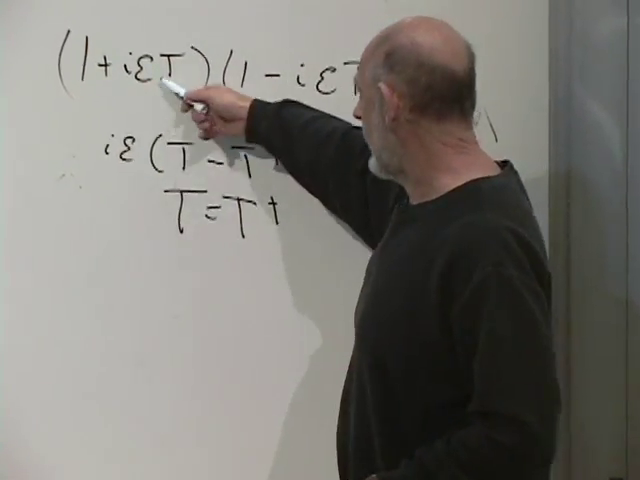
\includegraphics[width=0.62\textwidth]{lecture_04_figure_03.png}\caption{Die Unitaritätsrechnung nahe dem Einselement endet mit \(T=T^\dagger\).}\lectureframe{00:23:28}\end{figure}

Drei linear unabhängige Erzeugende entsprechen räumlichen Rotationen, denn es gibt drei unabhängige infinitesimale Achsen. Eine kleine Rotation um eine beliebige Richtung lässt sich aus kleinen Rotationen um \(x\), \(y\) und \(z\) zusammensetzen. Die entsprechenden Erzeugenden sind die Drehimpulsoperatoren \(J_x,J_y,J_z\). Ihre Kommutatoren kodieren die Nichtvertauschbarkeit von Rotationen:
\begin{equation}
[J_i,J_j]=i\epsilon_{ijk}J_k.
\label{eq:l4-angular-momentum-algebra}
\end{equation}
Durch wiederholte infinitesimale Rotationen entsteht dann eine endliche Rotation.

Wir haben die Unitarität verwendet, aber noch nicht die Bedingung, dass die Determinante eins ist. Für eine beliebige kleine Matrix \(m\) gilt
\begin{equation}
\det(\boldsymbol 1+\epsilon m)
=1+\epsilon\,\operatorname{tr}m+O(\epsilon^2).
\label{eq:l4-det-expansion}
\end{equation}

\begin{figure}[htbp]\centering
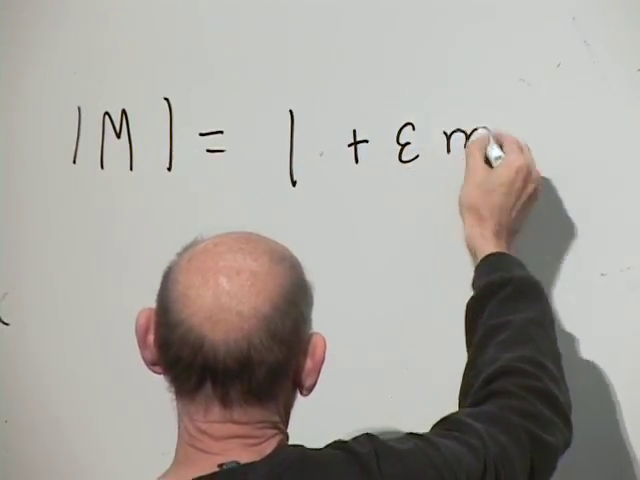
\includegraphics[width=0.62\textwidth]{lecture_04_figure_02.png}\caption{Die Entwicklung der Determinante in erster Ordnung, wie sie an der Tafel beginnt.}\lectureframe{00:21:51}\end{figure}

Wenden wir Gleichung~\eqref{eq:l4-det-expansion} auf Gleichung~\eqref{eq:l4-infinitesimal-u} an, so erhalten wir
\begin{equation}
\det U
=1+i\epsilon\,\operatorname{tr}T+O(\epsilon^2).
\end{equation}
Die Bedingung der speziellen Unitarität verlangt daher
\begin{equation}
\operatorname{tr}T=0.
\label{eq:l4-traceless-generator}
\end{equation}
Die Erzeugenden von \(SU(2)\) sind genau die spurfreien hermiteschen \(2\times2\)-Matrizen. Dieser Vektorraum hat Dimension drei. Eine Standardbasis bilden die Pauli-Matrizen:
\begin{equation}
\begin{aligned}
\sigma_x&=
\begin{pmatrix}0&1\\1&0\end{pmatrix},
&
\sigma_y&=
\begin{pmatrix}0&-i\\i&0\end{pmatrix},
\\[0.4em]
\sigma_z&=
\begin{pmatrix}1&0\\0&-1\end{pmatrix}.
\end{aligned}
\end{equation}
Für eine Spin-ein-Halb-Darstellung kann man \(J_i=\sigma_i/2\) wählen. Eine endliche Rotation um den Winkel \(\theta\) um die Richtung \(\hat{\boldsymbol n}\) lautet dann
\begin{equation}
U(\hat{\boldsymbol n},\theta)
=\exp\!\left(-i\theta\,
\hat{\boldsymbol n}\cdot\boldsymbol\sigma/2\right).
\end{equation}
\editorialnote{Die endliche Exponentialdarstellung vervollständigt die übliche Behandlung der infinitesimalen Erzeugenden. Die Quelle betont wiederholte kleine Rotationen, statt diese Formel ausdrücklich anzugeben.}

\begin{classroomqa}
\audiencequestion{Gibt es also drei unabhängige spurfreie hermitesche \(2\times2\)-Matrizen?
\lecturetimestamp{00:24:07}}
\lecturerresponse{Ja. Es sind die drei Pauli-Matrizen. Für spezielle unitäre \(3\times3\)-Matrizen beträgt die entsprechende Anzahl acht; eine konventionelle Basis bilden die acht Gell-Mann-Matrizen.}
\end{classroomqa}

\begin{classroomqa}
\audiencequestion{Ist diese ``Acht'' dieselbe wie beim Achtfachen Weg und bei den acht Gluonen?
\lecturetimestamp{00:24:43}}
\lecturerresponse{Die Mathematik beruht auf derselben Art von Darstellungstheorie \(SU(3)\), aber man muss angeben, welche Symmetrie \(SU(3)\) wirkt. Die historische Flavor-Symmetrie des Achtfachen Weges ist nicht die Farbsymmetrie \(SU(3)\). Die acht Gluonen gehören zur adjungierten Darstellung der Farbsymmetrie \(SU(3)\).}
\end{classroomqa}

\section{Von SU(2) zu Farb-SU(3)}

Vergrößern wir nun die Matrizen von \(2\times2\) auf \(3\times3\). Eine allgemeine komplexe \(3\times3\)-Matrix hat neun komplexe Einträge, also achtzehn reelle Parameter. Die Bedingung \(U^\dagger U=\boldsymbol 1\) liefert neun reelle Bedingungen, und \(\det U=1\) fügt eine weitere hinzu. Somit gilt
\begin{equation}
18-9-1=8.
\end{equation}
Es gibt acht unabhängige infinitesimale Richtungen und acht spurfreie hermitesche Erzeugende. Anders als \(SU(2)\) ist diese Gruppe nicht die Rotationsgruppe des gewöhnlichen dreidimensionalen Raums. Sie ist eine innere Symmetrie, die auf Farbe wirkt.

Bevor wir diese Darstellungen Quarks zuordnen, erinnern wir uns daran, wie zusammengesetzte Darstellungen entstehen. Legt man zwei Spin-ein-Halb-Systeme übereinander und lässt ihre Bahnbewegung außer Acht, erhält man vier Produktzustände. Eine Rotation mischt jedoch nicht alle vier unzerlegbar miteinander. Drei Kombinationen transformieren wie Spin eins:
\begin{align}
\ket{1,1}&=\ket{\uparrow\uparrow},\\
\ket{1,0}&=\frac{1}{\sqrt2}
(\ket{\uparrow\downarrow}+\ket{\downarrow\uparrow}),\\
\ket{1,-1}&=\ket{\downarrow\downarrow},
\end{align}
während die vierte wie Spin null transformiert:
\begin{equation}
\ket{0,0}=\frac{1}{\sqrt2}
(\ket{\uparrow\downarrow}-\ket{\downarrow\uparrow}).
\end{equation}
Damit gilt
\begin{equation}
\boldsymbol 2\otimes\boldsymbol 2
=\boldsymbol 3\oplus\boldsymbol 1.
\label{eq:l4-two-spin-decomposition}
\end{equation}
Die ausgerichteten Zustände bilden die Zustände mit \(m=\pm1\), der symmetrische Zustand mit Projektion null vervollständigt das Triplett, und die antisymmetrische Kombination ist das Singulett. Darin liegt die allgemeine Logik der Addition von Drehimpulsen und der Kombination von Farbdarstellungen.

Dieselbe Singulett--Triplett-Unterscheidung tritt immer auf, wenn zwei Spin-ein-Halb-Freiheitsgrade gekoppelt werden. Im atomaren Wasserstoff bilden Elektron- und Protonenspin Hyperfein-Singulett- und -Triplettzustände. Ortho- und Parawasserstoff verwenden dieselbe Darstellungstheorie für die Kernspins der beiden Protonen in einem \(H_2\)-Molekül.
\editorialnote{Die Quelle verwendet ``Ortho- und Parawasserstoff'' und bezieht sich dabei auf Proton--Elektron-Spins im Wasserstoffatom. Die mathematische Zerlegung ist korrekt; zur Präzisierung werden hier die Bezeichnungen für Molekül und Atom unterschieden.}

\subsection{Das Triplett und das Antitriplett}

Ein einzelnes Quark hat drei Farb-Amplituden. In einer gewählten Basis schreiben wir
\begin{equation}
q=
\begin{pmatrix}
q_r\\q_g\\q_b
\end{pmatrix},
\qquad
q'=Uq,
\qquad U\in SU(3).
\label{eq:l4-quark-triplet}
\end{equation}
Die drei Einträge können Zustandsamplituden eines einzelnen Quarks oder drei Feldoperatoren sein, die rote, grüne und blaue Quarks erzeugen. Die Gruppe mischt die drei Komponenten. Ein Zustand, der zunächst rot ist, wird nach einer Farbtransformation im Allgemeinen zu einer Überlagerung aus Rot, Grün und Blau. Diese fundamentale dreidimensionale Darstellung heißt \(\boldsymbol 3\).

Bei einem Antiquark wirkt die Gruppe durch die komplex konjugierte Darstellung der Quarkdarstellung. Die komplexe Konjugation von Gleichung~\eqref{eq:l4-quark-triplet} ergibt
\begin{equation}
\bar q'=U^*\bar q.
\end{equation}
Diese Darstellung wird mit \(\bar{\boldsymbol 3}\) bezeichnet. Die Analogie zu \(U(1)\) liegt auf der Hand: Nimmt ein Elektronenfeld den Faktor \(e^{i\theta}\) auf, so nimmt ein Positronenfeld \(e^{-i\theta}\) auf. Die Farbtransformationen von Quarks und Antiquarks bilden die nichtabelsche Variante dieser konjugierten Zuordnung.

Nahe dem Einselement gilt, wenn
\begin{equation}
U=\boldsymbol 1+i\epsilon T,
\end{equation}
dann
\begin{equation}
U^*=\boldsymbol 1-i\epsilon T^*.
\end{equation}
Die Erzeugenden des Antitripletts sind somit \(-T^*\), also die komplex konjugierten Erzeugenden mit umgekehrtem Vorzeichen. Genau in diesem Sinn tragen Antiquarks entgegengesetzte Farbladungen.

\begin{classroomqa}
\audiencequestion{Was geschieht mit der komplex konjugierten Darstellung im Fall \(SU(2)\)?
\lecturetimestamp{00:36:19}}
\lecturerresponse{Das \(SU(2)\)-Dublett ist ein Sonderfall: Seine komplex konjugierte Darstellung ist nach einer festen Basisänderung mit dem ursprünglichen Dublett äquivalent; diese verwendet den antisymmetrischen Epsilon-Tensor. Für \(SU(3)\) sind \(\boldsymbol 3\) und \(\bar{\boldsymbol 3}\) tatsächlich nicht äquivalente Darstellungen.}
\end{classroomqa}
\editorialnote{Der mathematisch präzise Begriff für die fundamentale Darstellung von \(SU(2)\) lautet pseudoreell, nicht reell. Die Antwort bewahrt die beabsichtigte Unterscheidung der Quelle und korrigiert zugleich die Terminologie.}

\section{Farbdarstellungen kombinieren}

Das Symbol \(\otimes\) bedeutet keine gewöhnliche Multiplikation der danebenstehenden Zahlen. Es bezeichnet die Kombination zweier Zustandsräume. Der entstehende Tensorproduktraum wird anschließend in Teilräume zerlegt, die unter der Gruppenwirkung nicht miteinander vermischt werden.

\subsection{\texorpdfstring{\(\boldsymbol 3\otimes\boldsymbol 3\)}{Zwei Quarks: 33 x }}

Zwei Quarks haben neun Farb-Basiszustände: Rot--Rot, Rot--Grün, Rot--Blau sowie die sechs übrigen geordneten Paare. Ordnen wir die beiden Farb-Indizes in einen symmetrischen und einen antisymmetrischen Anteil. Der symmetrische Anteil hat sechs unabhängige Komponenten, der antisymmetrische drei. Unter \(SU(3)\) gilt
\begin{equation}
\boldsymbol 3\otimes\boldsymbol 3
=\boldsymbol 6\oplus\bar{\boldsymbol 3}.
\label{eq:l4-three-times-three}
\end{equation}

\begin{figure}[htbp]\centering
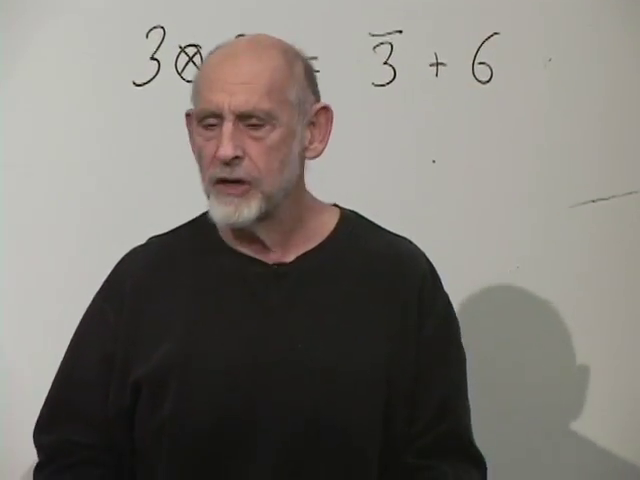
\includegraphics[width=0.68\textwidth]{lecture_04_figure_04.png}\caption{Das Produkt zweier Quarks zerfällt in ein Antitriplett und ein Sextett.}\lectureframe{00:39:33}\end{figure}

Das Antitriplett lässt sich ausdrücklich darstellen, indem man zwei Quark-Indizes mit dem invarianten Epsilon-Tensor kontrahiert:
\begin{equation}
(qq)^k_{\bar 3}
=\frac{1}{\sqrt2}\epsilon^{kij}q_iq_j.
\end{equation}
Dieses Objekt hat drei Komponenten und transformiert wie ein Antiquark. Die sechs symmetrischen Kombinationen bilden das Sextett. Die Aussage lautet nicht, dass sich zwei Quarks dynamisch in ein Antiquark verwandeln; vielmehr hat ein Sektor ihrer Farb-Wellenfunktion dasselbe Transformationsgesetz wie ein Antiquark.

\subsection{\texorpdfstring{\(\boldsymbol 3\otimes\bar{\boldsymbol 3}\)}{Ein Quark und ein Antiquark: 3 x Anti-3}}

Ein Quark--Antiquark-Farbzustand lässt sich als \(3\times3\)-Matrix \(M_i{}^j=q_i\bar q^j\) auffassen. Jede solche Matrix zerfällt eindeutig in ihre Spur und einen spurfreien Anteil:
\begin{equation}
M=\frac{\operatorname{tr}M}{3}\boldsymbol 1
+\left(M-\frac{\operatorname{tr}M}{3}\boldsymbol 1\right).
\end{equation}
Die Spur ist eine einzelne invariante Komponente, der spurfreie Anteil hat acht Komponenten. Daher gilt
\begin{equation}
\boldsymbol 3\otimes\bar{\boldsymbol 3}
=\boldsymbol 1\oplus\boldsymbol 8.
\label{eq:l4-three-times-threebar}
\end{equation}
Bis auf die Normierung lautet das Singulett
\begin{equation}
\ket{1}_{q\bar q}
=\frac{1}{\sqrt3}
(\ket{r\bar r}+\ket{g\bar g}+\ket{b\bar b}).
\end{equation}
Es kann in nichts anderes transformieren, weil es invariant ist. Die übrigen acht Linearkombinationen mischen sich untereinander. Sie bilden die adjungierte Darstellung, in der auch die acht Erzeugenden transformieren.

\subsection{Drei Quarks}

Kombinieren wir ein drittes Quark mit Gleichung~\eqref{eq:l4-three-times-three}. Der Antitriplett-Zweig ergibt
\begin{equation}
\bar{\boldsymbol 3}\otimes\boldsymbol 3
=\boldsymbol 1\oplus\boldsymbol 8,
\end{equation}
sodass das Produkt aus drei Quarks ein Singulett enthält. Vollständig lautet die Zerlegung
\begin{equation}
\boldsymbol 3\otimes\boldsymbol 3\otimes\boldsymbol 3
=\boldsymbol 1\oplus\boldsymbol 8\oplus\boldsymbol 8
\oplus\boldsymbol{10}.
\label{eq:l4-three-quark-full}
\end{equation}
Das Farbsingulett ist die vollständig antisymmetrische Kombination Rot--Grün--Blau:
\begin{equation}
\ket{1}_{qqq}
=\frac{1}{\sqrt6}\epsilon^{ijk}\ket{q_iq_jq_k}.
\label{eq:l4-baryon-singlet}
\end{equation}
Da \(\epsilon^{ijk}\) verschwindet, wenn zwei Indizes übereinstimmen, enthält jeder von null verschiedene Term genau ein rotes, ein grünes und ein blaues Quark; beim Vertauschen wechseln die Vorzeichen.

\begin{classroomqa}
\audiencequestion{Sind die Kombinationen, die keine Singuletts sind, lediglich unwahrscheinlich, sodass man ihre Wahrscheinlichkeiten vernachlässigen kann?
\lecturetimestamp{00:46:02}}
\lecturerresponse{Nein. Entscheidend ist die Energie, nicht eine geringe Wahrscheinlichkeit. Ein isolierter Zustand, der kein Singulett ist, hätte ein Farbfeld, das bis in beliebig große Entfernung reicht, und würde im Confinement-Bereich unbegrenzte Energie erfordern. Die Dynamik dahinter behandeln wir weiter unten.}
\end{classroomqa}

\subsection{Das Gluonen-Oktett}

Das Gluonenfeld transformiert wie das Oktett in Gleichung~\eqref{eq:l4-three-times-threebar}. Bezüglich der Farbe trägt es einen Triplett- und einen Antitriplett-Index, wobei die Singulett-Spur entfernt ist. Schematisch gilt
\begin{equation}
q\sim\boldsymbol 3,
\qquad
\bar q\sim\bar{\boldsymbol 3},
\qquad
G\sim\boldsymbol 8.
\end{equation}
Diese Symbole bezeichnen Transformationsgesetze; Teilchen sind nicht wörtlich gleich den Zahlen drei und acht.

Die neunte Farb-Kombination aus Quark-- und Antiquark, proportional zur Einheitsmatrix, ist ein Singulett und mischt sich nicht mit dem Oktett. Sie wegzulassen ist daher mathematisch konsistent: Ein \(SU(3)\)-Eichfeld ist spurfrei und hat acht Komponenten, statt der neun eines \(U(3)\)-Eichfelds.

\begin{classroomqa}
\audiencequestion{Warum lässt die Natur das zusätzliche Singulett-Gluon weg?
\lecturetimestamp{00:49:00}}
\lecturerresponse{Die unmittelbare gruppentheoretische Antwort lautet, dass das Singulett ein eigener invarianter Sektor ist. Daher ist das Oktett auch ohne ihn abgeschlossen. Der tieferliegende Grund für die Wahl von \(SU(3)\) statt \(U(3)\) wird hier nicht hergeleitet; er gehört zur Eichstruktur, die aus der Phänomenologie der QCD erschlossen wird.}
\end{classroomqa}

\section{Farbsinguletts als Hadronen}

Die freien Teilchen endlicher Masse der starken Wechselwirkung sind Farbsinguletts. Das macht Quarks oder Gluonen nicht unwirklich, sondern bedeutet, dass sie nicht als isolierte asymptotische Teilchen auftreten. Die grundlegenden Muster zur Bildung von Singuletts sind
\begin{equation}
qqq,
\qquad
q\bar q,
\qquad
GG\ \text{and higher gluonic products}.
\end{equation}
Sie führen der Reihe nach zu Baryonen, Mesonen und Glueballs. Produkte mehrerer bereits farbloser Objekte sind natürlich ebenfalls farblos; aus diesen Bausteinen lassen sich daher auch komplexere Multihadron-Zustände bilden.

\begin{classroomqa}
\audiencequestion{Wie heißen die Singuletts aus drei Quarks und aus einem Quark--Antiquark, und können auch Gluonen Singuletts bilden?
\lecturetimestamp{00:51:38}}
\lecturerresponse{Ein Singulett aus drei Quarks heißt Baryon, ein Singulett aus Quark--Antiquark Meson. Auch Gluonen können sich zu Farbsinguletts verbinden. Die einfachsten solcher stark wechselwirkenden Zustände heißen Glueballs; daran können mehr als zwei Gluonen beteiligt sein.}
\end{classroomqa}

Drei Spin-ein-Halb-Quarks ergeben stets einen Gesamtspin, der eine halbzahlige ganze Zahl ist; der Bahndrehimpuls kann jedoch bestimmen, welche halbzahlige Zahl auftritt. Mesonen aus Quark--Antiquark haben ganzzahligen Spin. Rein gluonische Glueballs haben ebenfalls ganzzahligen Spin.

Die erste Aussage an der Tafel zu zwei Gluonen ist lediglich eine Zählung:
\begin{equation}
8\times8=1+63.
\end{equation}
Insgesamt gibt es vierundsechzig Farbzustände; eine Kombination ist ein Singulett, und die übrigen dreiundsechzig gehören zu Sektoren, die keine Singuletts sind.

\begin{figure}[htbp]\centering
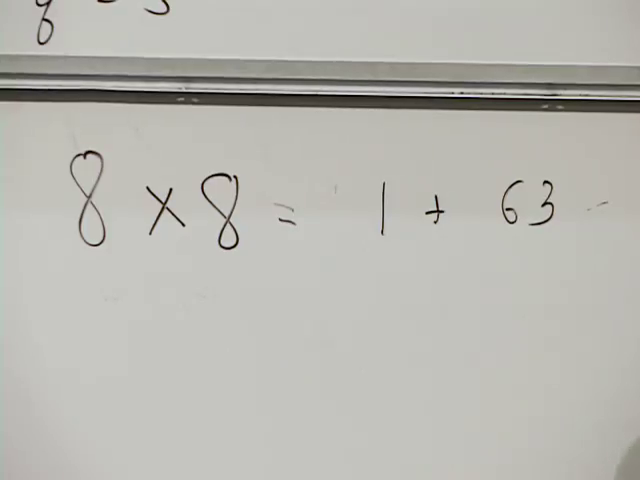
\includegraphics[width=0.68\textwidth]{lecture_04_figure_05.png}\caption{Die Zustandszählung an der Tafel für zwei Gluonen: ein Singulett unter vierundsechzig Zuständen.}\lectureframe{00:53:44}\end{figure}

Die vollständige Zerlegung in irreduzible Darstellungen lautet
\begin{equation}
\boldsymbol 8\otimes\boldsymbol 8
=\boldsymbol 1\oplus\boldsymbol 8_S\oplus\boldsymbol 8_A
\oplus\boldsymbol{10}\oplus\overline{\boldsymbol{10}}
\oplus\boldsymbol{27}.
\label{eq:l4-eight-times-eight}
\end{equation}
Die Dimensionen ergeben zusammen die richtige Gesamtzahl:
\begin{equation}
1+8+8+10+10+27=64.
\end{equation}
Die beiden Oktette sind verschiedene invariante Unterräume: Eines ist unter dem Austausch der beiden adjungierten Faktoren symmetrisch, das andere antisymmetrisch. Das Singulett ist der Farbkanal aus zwei Gluonen, aus dem ein Glueball-Zustand gebildet werden kann.
\editorialnote{An der Tafel steht zunächst nur \(8\times8=1+63\). Der spätere Austausch im Hörsaal ergänzt die angegebenen irreduziblen Dimensionen; Balken und Symmetrieindizes sind hier in der üblichen \(SU(3)\)-Notation wiedergegeben.}

\subsection{Warum beobachtbare elektrische Ladungen ganzzahlig sind}

Die Quarkladungen fallen in zwei Typen:
\begin{equation}
Q_{\mathrm{up\text{-}like}}=+\frac23,
\qquad
Q_{\mathrm{down\text{-}like}}=-\frac13.
\end{equation}
Drei Quarks haben daher eine ganzzahlige Gesamtladung: \(-1,0,+1,\text{ or }+2\), je nachdem, wie viele davon up-artig sind. Ein Quark und ein Antiquark haben ebenso eine Ladung von \(0\) oder \(\pm1\). Gluonen tragen keine elektrische Ladung. Somit haben die grundlegenden Farbsinguletts, die sich aus den beobachteten Quarkdarstellungen bilden, ganzzahlige elektrische Ladung, obwohl ihre Bestandteile gebrochene Ladungen tragen.

\begin{classroomqa}
\audiencequestion{Welche elektrische Ladung hat das Strange-Quark?
\lecturetimestamp{00:56:08}}
\lecturerresponse{Es ist down-artig und hat daher die Ladung \(-1/3\). Die drei Familien wiederholen dasselbe Ladungsmuster: \((u,d)\), \((c,s)\) und \((t,b)\); jedes Paar hat die Ladungen \(+2/3\) und \(-1/3\).}
\end{classroomqa}

Für diesen Teilcheninhalt hängen Farbsingulett-Eigenschaft und ganzzahlige elektrische Ladung eng zusammen, sind aber mathematisch nicht dasselbe. Die Ganzzahligkeit folgt auch aus den gerade angegebenen elektrischen Ladungszuordnungen des Standardmodells.

\begin{classroomqa}
\audiencequestion{Ist ein Farbsingulett ein verschränkter Zustand, und hat diese Verschränkung dieselbe Bedeutung wie die eines verschränkten Paares in einem Bell-Experiment?
\lecturetimestamp{00:56:58}}
\lecturerresponse{Die Farbsingulett-Wellenfunktion ist tatsächlich verschränkt: Sie ist eine kohärente Überlagerung und kein Produkt von Zuständen mit jeweils bestimmter Farbe. Grundsätzlich lassen sich ihre Bestandteile voneinander trennen, doch aufgrund des Confinements wird diese Trennung zunehmend aufwendiger und führt schließlich zur Bildung neuer Hadronen. Daher eignet sich der Zustand nicht für eine Manipulation nach Art eines Bell-Experiments, obwohl er verschränkt ist.}
\end{classroomqa}

\section{Was die Tensorprodukt-Gleichungen bedeuten}

An dieser Stelle verdienen die Multiplikationstafeln eine anschaulichere Erklärung. Seien \(\psi_i\) und \(\phi_j\) Operatoren, die zwei Spin-ein-Halb-Objekte erzeugen. Sie können zwei Teilchensorten wie ein Elektron und ein Proton beschreiben oder, unter Berücksichtigung der passenden Statistik, zwei Exemplare derselben Sorte. Jeder Index kann zwei Werte annehmen. Die vier Produkte
\begin{equation}
\psi_\uparrow\phi_\uparrow,
\quad
\psi_\uparrow\phi_\downarrow,
\quad
\psi_\downarrow\phi_\uparrow,
\quad
\psi_\downarrow\phi_\downarrow
\end{equation}
spannen den Tensorproduktraum auf.

Wirkt ein Gruppenelement auf jeden Faktor wie \(U\), so wirkt es auf das Produkt wie \(U\otimes U\). In Komponenten gilt
\begin{equation}
\psi_i\phi_j
\longmapsto
U_i{}^kU_j{}^\ell\psi_k\phi_\ell.
\label{eq:l4-product-action}
\end{equation}
Dies ist eine vierdimensionale, aber reduzible Darstellung. Die antisymmetrische Kombination
\begin{equation}
\frac{1}{\sqrt2}
(\psi_\uparrow\phi_\downarrow
-\psi_\downarrow\phi_\uparrow)
\end{equation}
wird in sich selbst abgebildet, während die drei symmetrischen Kombinationen untereinander abgebildet werden. In einer an diese Kombinationen angepassten Basis hat jede Matrix der Produktdarstellung Blockdiagonalform:
\begin{equation}
D_{2\otimes2}(g)
\sim
\begin{pmatrix}
1&0\\
0&D_3(g)
\end{pmatrix}.
\label{eq:l4-spin-block-diagonal}
\end{equation}

\begin{classroomqa}
\audiencequestion{Welche Operation stellt eine Gleichung wie \(\boldsymbol 3\otimes\boldsymbol 3=\bar{\boldsymbol 3}\oplus\boldsymbol 6\) dar?
\lecturetimestamp{00:57:51}}
\lecturerresponse{Die linke Seite bildet den zusammengesetzten Zustandsraum. Die Gruppe wirkt auf beide Faktoren und mischt daher die Produktbasiszustände. Die rechte Seite besagt, dass eine Basisänderung diese Zustände in invariante Mengen aufteilt: drei antisymmetrische Kombinationen, die wie ein Antitriplett transformieren, und sechs symmetrische Kombinationen, die wie ein Sextett transformieren. Das Pluszeichen bezeichnet eine direkte Summe von Möglichkeiten, keine gewöhnliche numerische Addition.}
\end{classroomqa}

\begin{classroomqa}
\audiencequestion{Woher wissen wir, dass sich die neun Zustände als \(3+6\) oder als \(1+8\) zerlegen und nicht etwa als \(2+7\)?
\lecturetimestamp{01:04:39}}
\lecturerresponse{Die Dimensionszählung allein entscheidet nicht über die Zerlegung. Man muss wissen, welche irreduziblen Darstellungen \(SU(3)\) besitzt, und invariante Unterräume konstruieren, etwa indem man Indizes symmetrisiert oder antisymmetrisiert oder Spur und spurfreie Anteile trennt. Eine vollständige Klassifikation erfordert mehr Gruppentheorie; hier verwenden wir nur die für Quarks und Gluonen benötigten Darstellungen.}
\end{classroomqa}

Der invariante Epsilon-Tensor macht die Konstruktion des Singuletts anschaulich. Für \(SU(2)\) gilt
\begin{equation}
\epsilon_{ij}U^i{}_kU^j{}_\ell
=(\det U)\epsilon_{k\ell}
=\epsilon_{k\ell}.
\end{equation}
Daher ist \(\epsilon_{ij}\psi^i\phi^j\) invariant. Für \(SU(3)\) ergibt die Variante mit drei Indizes
\begin{equation}
\epsilon_{ijk}U^i{}_aU^j{}_bU^k{}_c
=(\det U)\epsilon_{abc}
=\epsilon_{abc},
\end{equation}
und beweist damit die Invarianz des Drei-Quark-Zustands in Gleichung~\eqref{eq:l4-baryon-singlet}.

\begin{classroomqa}
\audiencequestion{Kann man ausdrücklich zeigen, warum das Singulett nicht transformiert?
\lecturetimestamp{01:07:18}}
\lecturerresponse{Ja. Kontrahiere alle fundamentalen Indizes mit dem vollständig antisymmetrischen Epsilon-Tensor. Bei der Transformation multipliziert das Produkt der Matrizen Epsilon mit \(\det U\). Für eine spezielle unitäre Matrix ist diese Determinante eins, sodass der kontrahierte Zustand unverändert bleibt. Für \(SU(2)\) beweist dies die Zwei-Spin-Singulett-Eigenschaft; für \(SU(3)\) die des Drei-Quark-Singuletts Rot--Grün--Blau.}
\end{classroomqa}

\begin{classroomqa}
\audiencequestion{Wie lautet die vollständige Zerlegung zweier Gluonen-Oktette?
\lecturetimestamp{01:09:24}}
\lecturerresponse{Sie ist die Zerlegung aus Gleichung~\eqref{eq:l4-eight-times-eight}: ein Singulett, zwei Oktette, ein Dekuplett, ein Antidekuplett und eine Darstellung der Dimension siebenundzwanzig. Es gibt genau eine farbsinguläre Kombination der beiden Oktett-Indizes.}
\end{classroomqa}

\begin{classroomqa}
\audiencequestion{Wie lautet die entsprechende vollständige Zerlegung für drei Quarks?
\lecturetimestamp{01:11:51}}
\lecturerresponse{Die physikalisch wesentliche Antwort ist, dass sie ein Singulett enthält. Ergänzt man die vollständige Zerlegung, erhält man Gleichung~\eqref{eq:l4-three-quark-full}: ein Singulett, zwei Oktette und ein Dekuplett, insgesamt also \(1+8+8+10=27\) Zustände.\editorialnote{Während des Austauschs kann sich der Dozent nicht an die vollständige Zerlegung \(3\otimes3\otimes3\) erinnern. Die übliche Ergänzung wird hier ausdrücklich angegeben und nicht der gesprochenen Antwort zugeschrieben.}}
\end{classroomqa}

Dieselbe Idee lässt sich auf den Zweigluonenraum übertragen. In der naiven Produktbasis wirkt \(SU(3)\) durch \(64\times64\)-Matrizen. In einer an die irreduziblen Komponenten angepassten Basis sind diese Matrizen blockdiagonal,
\begin{equation}
\begin{aligned}
D_{8\otimes8}(g)
&\sim
\operatorname{diag}\bigl(
1,D_{8_S}(g),D_{8_A}(g),
\\
&\hspace{4.8em}
D_{10}(g),D_{\overline{10}}(g),D_{27}(g)
\bigr).
\end{aligned}
\end{equation}
Kein Block mischt sich mit einem anderen, obwohl sich die Zustände innerhalb jedes Blocks untereinander mischen.

\begin{classroomqa}
\audiencequestion{Ist die Zerlegung des Tensorprodukts also einfach ein Basiswechsel, bei dem die große Darstellungsmatrix blockdiagonal wird?
\lecturetimestamp{01:12:02}}
\lecturerresponse{Genau. Bei zwei Spins zerfällt die vierdimensionale Matrix in einen eindimensionalen Singulettblock und einen dreidimensionalen Triplettblock. Bei zwei Gluonen zerfällt die 64-dimensionale Matrix in Blöcke der Dimensionen \(1,8,8,10,10,\text{ and }27\). Jeder Block ist unter jeder Gruppentransformation abgeschlossen.}
\end{classroomqa}

\begin{classroomqa}
\audiencequestion{Gibt es eine Bezeichnung für eines dieser abgeschlossenen Teilstücke im gesamten Tensorproduktraum?
\lecturetimestamp{01:14:55}}
\lecturerresponse{Es ist ein invarianter Unterraum, der eine Unterdarstellung trägt. Lässt es sich nicht weiter zerlegen, trägt es eine irreduzible Darstellung, kurz Irrep. Das gesamte Tensorprodukt ist die direkte Summe dieser irreduziblen Komponenten.\editorialnote{Im Ausgangstext bleibt der gesuchte Begriff im Hörsaal unbeantwortet. Die Antwort ergänzt den gebräuchlichen Begriff aus der Darstellungstheorie.}}
\end{classroomqa}

\begin{classroomqa}
\audiencequestion{Wenn die Nichtsingulett-Dekupletts und andere Darstellungen als nicht existent bezeichnet werden, heißt das, dass man sie vollständig ignorieren sollte?
\lecturetimestamp{01:15:36}}
\lecturerresponse{Sie sind zulässige Farbsektoren und spielen in Zwischenrechnungen eine Rolle, treten im Labor aber nicht als isolierte Teilchen endlicher Energie auf. Nicht ein Versagen der Darstellungstheorie, sondern das Confinement verhindert, dass sie zu freien asymptotischen Zuständen werden.}
\end{classroomqa}

\section{Von Nambus Farbidee zum Confinement}

Die Farbidee entstand vor der endgültigen Formulierung der QCD. Yoichiro Nambu erkannte bereits in den frühen 1960er Jahren, dass eine verborgene dreifachwertige Quantenzahl ein verblüffendes Problem lösen könnte: Quarks tragen eine gebrochene elektrische Ladung, doch freie Teilchen mit gebrochener Ladung werden nicht beobachtet. Wenn physikalische Zustände auf Farbsinguletts beschränkt sind, treten Quarks in den oben beschriebenen Kombinationen mit ganzzahliger Ladung auf. Die verbleibende Frage ist dynamischer Natur: Welche Kräfte zwingen alle freien Zustände endlicher Energie, Singuletts zu sein?

Beginnen wir mit der Analogie zur Elektromagnetismus. Eine Ladung und eine entgegengesetzte Ladung ziehen sich an. Bringt man sie zusammen, sinkt die Energie; gleichnamige Ladungen zusammenzuschieben erfordert Arbeit. Das Feld selbst speichert positive Energie,
\begin{equation}
E_{\mathrm{field}}
=\frac12\int d^3x\,\boldsymbol E^2
\end{equation}
in einfachen elektrostatischen Einheiten. Bei einer Nettoladung reicht das Feld weit über das System hinaus, während ein eng gebundenes neutrales Paar nur ein Dipolfeld kurzer Reichweite besitzt. Durch die Neutralisierung wird daher Feldenergie aus dem Außenraum entfernt.

Stellen wir uns vor, die elektromagnetische Kopplung würde enorm vergrößert. Die Feldenergiekosten einer Nettoladung würden so hoch, dass Objekte niedriger Energie überwiegend neutral wären und das Herauslösen eines geladenen Bestandteils unerschwinglich teuer werden könnte. Nambu übertrug diese Vorstellung auf die Farbe: Die acht Farbladungen sind Quellen von acht Gluonenfeldern, sodass eine große Farbfeldenergie isolierte Nichtsinguletts ausschließen könnte.

Diese Vorstellung trifft im Wesentlichen zu, doch die QCD weist ein entscheidendes neues Merkmal auf. Das Photon trägt keine elektrische Ladung, das Gluon hingegen Farbe. Das Photon ist keine Quelle des klassischen elektromagnetischen Feldes, und die Maxwell-Gleichungen sind linear: Zwei elektromagnetische Wellen überlagern sich und durchdringen einander. Ein Gluon transformiert in der Farboktett-Darstellung, daher sind Gluonen Quellen anderer Gluonen und wechselwirken mit ihnen. Auch verschiedene Teile eines einzelnen Gluonenfeldes wechselwirken miteinander. Das nichtabelsche Eichfeld ist deshalb nichtlinear.

\subsection{Flussschläuche und ein lineares Potenzial}

Auf großen Distanzen verhindert die Selbstwechselwirkung der Gluonen, dass sich der Farbfluss wie das gewöhnliche elektrische Dipolfeld ausbreitet. Der Fluss wird in einen Schlauch eingeschnürt, der ein Quark mit einem Antiquark verbindet. Feldstärke und Querschnittsfläche eines langen Schlauchs sind näherungsweise konstant, sodass der Schlauch näherungsweise eine konstante Energie pro Längeneinheit speichert. Bezeichnet \(\sigma\) die Stringspannung, so gilt
\begin{equation}
V(R)\simeq\sigma R+\text{constant}
\qquad (R\ \text{large}).
\label{eq:l4-linear-potential}
\end{equation}

\begin{figure}[htbp]
\centering
\includegraphics[width=0.78\textwidth]{lecture_04_figure_06.png}
\caption{In einem langen Schlauch gebündelter Farbfluss zwischen einem Quark und einem Antiquark.}
\lectureframe{01:31:35}
\end{figure}

Dies ist stärker als das Coulomb-Potenzial, dessen Betrag wie \(1/R\) abnimmt. Zieht man die Farbquellen weiter auseinander, wird die Kraft nicht immer schwächer; der Schlauch wird länger und seine Energie nimmt weiter zu. Eine einzelne Farbladung in einem unendlichen Volumen würde einen endlos langen Schlauch erfordern und damit unbeschränkte Energie. Das ist die physikalische Bedeutung der Aussage, dass nur Farbsinguletts asymptotische Zustände endlicher Energie sind.
\editorialnote{Die Notation für die Stringspannung und das explizite langreichweitige Potenzial machen die Aussage der Quelle quantitativ, dass ein gleichförmiger Flussschlauch eine gleichförmige Energie pro Längeneinheit trägt.}

\subsection{Stringbruch und Jets}

Nehmen wir an, eine harte Kollision trifft ein Quark in einem Meson. Das Quark beginnt sich fortzubewegen, doch hinter ihm spannt sich der Flussschlauch. Es kann seine kinetische Energie verlieren und zurückgezogen werden. Häufiger erzeugt das Vakuum, sobald die gespeicherte Feldenergie groß genug ist, ein neues Quark--Antiquark-Paar. Das neue Antiquark beendet den Fluss, der mit dem entkommenden Quark verbunden ist, während das neue Quark den Fluss zum ursprünglichen Antiquark beendet. Aus einem gedehnten Singulett werden zwei kürzere Singuletts,
\begin{equation}
(q\bar q)_{\mathrm{stretched}}
\longrightarrow
(q\bar q)+(q\bar q).
\label{eq:l4-string-breaking}
\end{equation}

\begin{figure}[htbp]
\centering
\includegraphics[width=0.78\textwidth]{lecture_04_figure_07.png}
\caption{Paarerzeugung bricht einen gedehnten Flussschlauch in zwei farbsingulettartige Schläuche auf.}
\lectureframe{01:34:52}
\end{figure}

\begin{classroomqa}
\audiencequestion{Was kann noch geschehen, wenn ein getroffenes Quark genug Energie hat, um den Schlauch weiter zu dehnen, außer dass es zurückgezogen wird?
\lecturetimestamp{01:33:50}}
\lecturerresponse{Der Schlauch kann durch die Erzeugung eines Quark--Antiquark-Paares aufbrechen. Seine Energie wird zur Masse und kinetischen Energie des neuen Paares. Die Endpunkte verbinden sich neu zu zwei Singuletts, sodass der Prozess zusätzliche Mesonen statt eines isolierten Quarks erzeugt.}
\end{classroomqa}

Wenn eines dieser Partonen weiterhin großen Impuls trägt, wiederholt sich der Prozess. Das Ergebnis ist eine Kaskade von farbsingulettartigen Hadronen, die um die ursprüngliche Partonrichtung gebündelt sind: ein Jet. Diese Umwandlung energiereicher Quarks und Gluonen in Hadronen heißt Hadronisierung. Auf das initiierende farbgeladene Objekt schließt man aus dem Jet, beobachtet wird es niemals für sich allein.

\begin{classroomqa}
\audiencequestion{Entstehen beim Stringbruch nur Mesonen, oder können im Jet auch andere Hadronen auftreten?
\lecturetimestamp{01:35:20}}
\lecturerresponse{Gewiss können auch andere Hadronen auftreten. Die einzige Farbanforderung ist, dass die letztlich beobachtbaren Objekte Singuletts sind. Mesonen sind das einfachste Bild für einen einzelnen Bruch, doch es können auch Baryonen, Antibaryonen und kompliziertere Singulettkombinationen entstehen.}
\end{classroomqa}

Drei Quarks können ihren Fluss an einem farbsingulettartigen Knotenpunkt beenden. Das Bild mit den drei Strängen ist das dynamische Gegenstück zum antisymmetrischen Epsilon-Tensor in Gleichung~\eqref{eq:l4-baryon-singlet}: Aus dem vollständigen Baryon tritt kein Nettofarbfluss aus.

\begin{figure}[htbp]
\centering
\includegraphics[width=0.72\textwidth]{lecture_04_figure_08.png}
\caption{Ein dreisträngiger Farbfluss-Knotenpunkt für ein Baryon, unterhalb der Skizze zum Stringbruch bei Mesonen.}
\lectureframe{01:36:12}
\end{figure}

\section{Eichfelder, Erhaltungsgrößen und das Standardmodell}

Auf der hier betrachteten Ebene lässt sich eine Eichtheorie als Theorie erkennen, in der eine erhaltene Ladung eine photonartige Feldquelle ist. Die elektrische Ladung ist Quelle des elektromagnetischen Feldes; die acht Farbladungen sind Quellen der acht Gluonenfelder. In der tiefer gehenden Formulierung wird die Symmetrie lokal gemacht und eine Verbindung eingeführt, die innere Zustände an benachbarten Raumzeitpunkten vergleicht. Diese Konstruktion wird für das hier entwickelte Bild des Confinements jedoch nicht benötigt.
\editorialnote{Die Formulierung mit lokaler Symmetrie ist die gebräuchliche tiefer gehende Bedeutung von Eichtheorie, auf die die Quelle anspielt, deren Erörterung sie aber bewusst aufschiebt.}

Symmetrie, erhaltene Ladung und Fluss hängen eng zusammen. Können Feldlinien nur an Ladungen enden, kann eine Quelle nicht einfach verschwinden, während ihr Fluss an nichts mehr gebunden ist. Auch kann ihr entferntes Feld nicht augenblicklich vollständig verschwinden, denn Änderungen des Feldes breiten sich kausal aus. In lokaler Form wird dieselbe Physik durch eine Kontinuitätsgleichung ausgedrückt,
\begin{equation}
\frac{\partial\rho}{\partial t}
+\boldsymbol\nabla\cdot\boldsymbol j=0,
\end{equation}
die besagt, dass Ladung ein Gebiet nur verlassen kann, indem sie dessen Grenze durchströmt. Das Bild der Feldlinien ist die geometrische Darstellung dieses lokalen Erhaltungsgesetzes.

Nun können wir das Ergebnis im Standardmodell verorten. Die Farbe umfasst die acht Generatoren von \(SU(3)\) und ihre acht Gluonenfelder. Der abelsche Sektor enthält einen Generator und ein Eichfeld. Drei weitere Generatoren gehören zu einer zusätzlichen \(SU(2)\), nicht zum gewöhnlichen räumlichen Drehimpuls. Vor der Symmetriebrechung lautet die Eichstruktur
\begin{equation}
SU(3)_c\times SU(2)_L\times U(1)_Y,
\end{equation}
mit \(8+3+1=12\) Generatoren. Als Nächstes gilt es, die elektroschwache \(SU(2)\) zu verstehen, dann das Higgs-Feld und die Entstehung des beobachteten Photons, von \(W^\pm\) und \(Z\).
\editorialnote{Die Quelle zählt das Photon zusammen mit den acht Gluonen und beschreibt den verbleibenden Faktor als \(SU(2)\times U(1)\). Im ungebrochenen Standardmodell ist der abelsche Faktor die Hyperladung \(U(1)_Y\); das Photon entsteht erst durch die elektroschwache Mischung.}

Die zentrale Argumentationskette ist nun vollständig. Abstrakte Gruppen wirken durch Darstellungen; infinitesimale Generatoren sind die erhaltenen Ladungen; Quarks, Antiquarks und Gluonen gehören zur \(\boldsymbol 3\)-, \(\bar{\boldsymbol 3}\)- beziehungsweise \(\boldsymbol 8\)-Darstellung; Tensorprodukte identifizieren die singulettartigen Hadronen; und das nichtlineare Gluonenfeld macht aus der Singulettauswahl das physikalische Phänomen des Confinements.

\chapter{Eichfelder, Wechselwirkungsskalen und geladene schwache Ströme}

Quantenelektrodynamik und Quantenchromodynamik sehen im Labor sehr unterschiedlich aus, doch beide sind Eichtheorien. Tatsächlich ist nahezu jede Wechselwirkung im Standardmodell auf diese Weise organisiert. Das Wort \emph{Eich} hat eine tiefere Bedeutung, die lokale Symmetrie einschließt; auf diesen Formalismus können wir jedoch zunächst verzichten. Für den Augenblick genügt eine minimale physikalische Beschreibung: Eine Eichtheorie enthält Maxwell-artige Felder, erhaltene Quellen, Symmetrietransformationen, Eichbosonen und Regeln für die Emission und Absorption dieser Bosonen.

\section{Die Maxwell-Theorie als Prototyp}

\subsection{Felder und Potentiale}

Das elektromagnetische Feld hat sechs Komponenten: drei Komponenten des elektrischen Feldes und drei des magnetischen Feldes. Dieselbe Information lässt sich mit einer gewissen Redundanz in einem Vierer-Vektorpotenzial kodieren
\begin{equation}
A_\mu=(A_0,\boldsymbol A),
\end{equation}
wobei \(A_0\) das elektrostatische Potenzial und \(\boldsymbol A\) das räumliche Vektorpotenzial ist. Im elektrostatischen Grenzfall erhält man das elektrische Feld aus dem räumlichen Gradienten,
\begin{equation}
\boldsymbol E=-\boldsymbol\nabla A_0,
\qquad
\boldsymbol F=q\boldsymbol E,
\end{equation}
während das magnetische Feld gegeben ist durch
\begin{equation}
\boldsymbol B=\boldsymbol\nabla\times\boldsymbol A.
\end{equation}
Das Vorzeichen in der ersten Gleichung hängt von der üblichen Definition des Potenzials ab; in der Tafelbesprechung geht es vor allem darum, dass die Felder Ableitungen der Potenziale sind.
\editorialnote{Für zeitabhängige Felder lautet die vollständige Beziehung
\(\boldsymbol E=-\boldsymbol\nabla A_0-\partial_t\boldsymbol A\). Hier beschränkt sich die Vorlesung bewusst auf den einfacheren elektrostatischen Fall.}

\begin{figure}[htbp]\centering
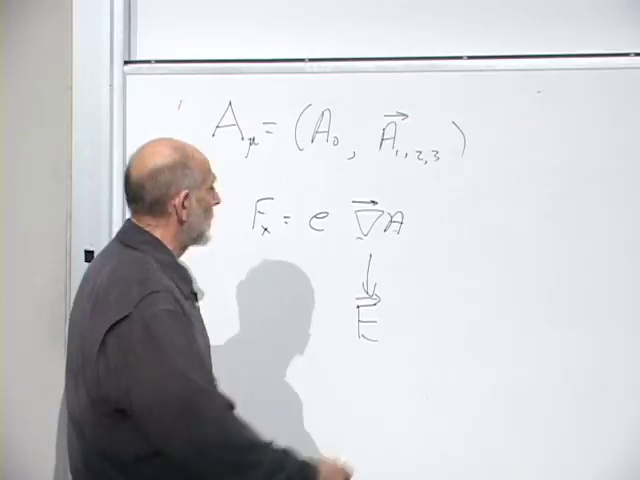
\includegraphics[width=0.62\textwidth]{lecture_05_figure_02.png}\caption{Das elektromagnetische Viererpotenzial und seine Ableitungsbeziehung zum Feld.}\lectureframe{00:03:33}\end{figure}

Damit gibt es in der Elektrodynamik zwei gleichwertige Beschreibungen: eine durch \(\boldsymbol E\) und \(\boldsymbol B\) und eine durch \(A_\mu\). Die zweite enthält nur vier angegebene Komponenten, weil verschiedene Potenziale dieselben physikalischen Felder beschreiben können. Diese Redundanz ist ein erster Hinweis auf die Bedeutung des Wortes Eichung, auch wenn wir den Begriff vorerst noch nicht formal verwenden.

\subsection{Wellen und Polarisation}

Die Maxwell-Gleichungen lassen Wellen zu. Betrachten wir eine ebene Welle, die sich entlang des Einheitsvektors \(\hat{\boldsymbol k}\) ausbreitet. An jedem Punkt stehen die elektrischen und magnetischen Felder quer zur Ausbreitungsrichtung:
\begin{equation}
\boldsymbol E\cdot\hat{\boldsymbol k}=0,
\qquad
\boldsymbol B\cdot\hat{\boldsymbol k}=0,
\qquad
\boldsymbol E\cdot\boldsymbol B=0.
\end{equation}
In Einheiten mit \(c=1\) sind ihre Beträge gleich:
\begin{equation}
|\boldsymbol E|=|\boldsymbol B|.
\end{equation}
Bei einer linear polarisierten Welle legt die Richtung von \(\boldsymbol E\) die Polarisation fest. Das gesamte Muster breitet sich mit Lichtgeschwindigkeit aus.

Die Quantisierung ändert die Beschreibung, aber nicht die Polarisationsstruktur. Ein Quant der elektromagnetischen Welle ist ein Photon. Ein Photon als Punkt darzustellen, ist zwangsläufig irreführend; dennoch kann man sich vorstellen, dass der Punkt einen kleinen, quer zur Ausbreitungsrichtung stehenden Zeiger trägt, der seine Polarisation angibt. Eine Viertelwellenplatte oder ein anderes optisches Element kann diese Polarisation drehen. Auch ein statisches Coulomb-Feld lässt sich, wenn auch nur grob, so auffassen, als entstehe es durch wiederholte Emission und Absorption von Photonen.

\subsection{Quellen, Fluss und Erhaltung}

Elektromagnetische Wellen können sich im leeren Raum ausbreiten, doch das Feld hat auch Quellen: elektrische Ladungen und Ströme. Eine positive Punktladung erzeugt ein radial nach außen gerichtetes elektrisches Feld, dessen Stärke proportional zu \(1/r^2\) ist. Die Zahl der Feldlinien, die eine beliebige Kugel um die Ladung durchstoßen, ist unabhängig vom Radius der Kugel. Mathematisch gilt in SI-Einheiten:
\begin{equation}
\oint_{S^2}\boldsymbol E\cdot d\boldsymbol S
=\frac{Q_{\mathrm{enc}}}{\epsilon_0},
\label{eq:l5-gauss}
\end{equation}

Das ist mehr als eine praktische Methode, das Feld zu berechnen. Elektrische Feldlinien können nur an Ladungen enden. Würde eine einzelne isolierte Ladung einfach verschwinden, müsste entweder ihr Feld überall gleichzeitig verschwinden, was der Kausalität widerspräche, oder eine Front des fehlenden Feldes müsste sich nach außen ausbreiten, wobei Feldlinien im leeren Raum endeten. Beides ist unzulässig. Die Geometrie des Flusses macht die Ladungserhaltung daher plausibel: Ladung kann sich bewegen, und entgegengesetzte Ladungen können annihilieren, aber die Nettoladung kann nicht lokal ohne einen kompensierenden Strom verschwinden.

Die entsprechende lokale Aussage ist die Kontinuitätsgleichung
\begin{equation}
\partial_t\rho+\boldsymbol\nabla\cdot\boldsymbol J=0.
\label{eq:l5-continuity}
\end{equation}
\editorialnote{~\eqref{eq:l5-continuity} ist die übliche lokale mathematische Form des Kausalitätsarguments über den Fluss, das in der Vorlesung verbal entwickelt wird.}

\subsection{Eine Arbeitsdefinition der Eichtheorie}

Wir können das Grundmuster nun operational formulieren. Eine Eichtheorie umfasst:
\begin{itemize}\item elektrizitätsartige und magnetismusartige Felder;
\item Wellen, die bei hinreichend schwachen Wechselwirkungen Lichtwellen ähneln;
\item Quellen, die der elektrischen Ladung entsprechen;
\item ein Gaußsches Gesetz, das den Fluss mit diesen Quellen verknüpft;
\item ein Erhaltungsgesetz und eine zugehörige Symmetrie;
\item Quanten des Feldes, sogenannte Eichbosonen; und
\item eine Kopplungskonstante, die Emission und Absorption bestimmt.
\end{itemize}
Die Quelle muss keine elektrische Ladung sein. Als bewusst unphysikalisches Beispiel stellen wir uns vor, die Baryonenzahl wäre eine Eichladung. Protonen und Neutronen haben beide die Baryonenzahl \(+1\), sodass sie sich durch eine neue, Coulomb-artige Kraft abstoßen würden; ein Proton und ein Antiproton würden sich anziehen. Eine solche Theorie ist mathematisch denkbar, doch in der Natur gibt es kein beobachtetes langreichweitiges Eichfeld, das an die Baryonenzahl koppelt. Erhaltung allein garantiert keine Eichkraft.

Die elektrische Ladung geht tatsächlich mit einer Symmetrie einher. Für ein geladenes Materiefeld gilt
\begin{equation}
\psi(x)\longmapsto e^{i\theta}\psi(x).
\label{eq:l5-u1}
\end{equation}
Phasensymmetrie und Ladungserhaltung sind zwei Seiten derselben Struktur. Später können wir \(\theta\) von der Raumzeit abhängen lassen und sehen, weshalb das Potenzial \(A_\mu\) benötigt wird. Hier genügt die globale Transformation, um die erhaltene Ladung zu identifizieren.

\section{Die QCD als nichtabelsches Beispiel}

\subsection{Tripletts, Antitripletts und die Gluonmatrix}

In der Quantenchromodynamik trägt ein Quarkfeld einen FarbindIndex \(i\in\{r,g,b\}\) und transformiert in der fundamentalen Darstellung von \(SU(3)\):
\begin{equation}
q'_i=U_{ij}q_j,
\qquad
U^\dagger U=\boldsymbol 1,
\qquad
\det U=1.
\label{eq:l5-q-transform}
\end{equation}
Dies ist eine Drehung in einem dreidimensionalen komplexen Farbraum, keine Drehung des gewöhnlichen Ortsraums. Die dreikomponentige Darstellung wird auch definierende Darstellung genannt.

Antiteilchenfelder werden durch die komplex konjugierten Variablen dargestellt. Die komplexe Konjugation von Gleichung~\eqref{eq:l5-q-transform} ergibt
\begin{equation}
q_i^{\prime *}=U_{ij}^*q_j^*.
\label{eq:l5-antiquark-transform}
\end{equation}
Quarks transformieren also gemäß \(\boldsymbol 3\), Antiquarks dagegen gemäß \(\bar{\boldsymbol 3}\).

\begin{figure}[htbp]\centering
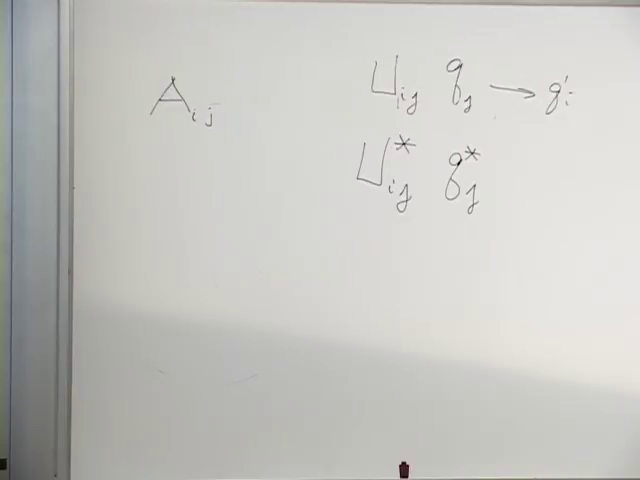
\includegraphics[width=0.62\textwidth]{lecture_05_figure_03.png}\caption{Die fundamentale Transformation und ihre komplex konjugierte Antitriplett-Transformation.}\lectureframe{00:18:47}\end{figure}

\begin{classroomqa}\audiencequestion{Wie viele \(U\)-Matrizen gibt es-- sieben, acht oder neun?
\lecturetimestamp{00:19:37}}\lecturerresponse{Es gibt unendlich viele Gruppenelemente \(U\). Gezählt wird die endliche Zahl der unabhängigen Generatoren; für \(SU(3)\) sind es acht. Eine allgemeine \(3\times3\)-Matrix hat neun Matrixeinträge, doch die spezielle Unitarität lässt acht kontinuierliche Richtungen übrig.}\end{classroomqa}

Das Gluonfeld lässt sich als spurlose Matrix \(A_{ij}\) schreiben. Ein Index transformiert wie ein Quark, der andere wie ein Antiquark; seine Farbstruktur entspricht daher
\begin{equation}
\boldsymbol 3\otimes\bar{\boldsymbol 3}
=\boldsymbol 1\oplus\boldsymbol 8.
\end{equation}
Die QCD behält das spurlose Oktett bei,
\begin{equation}
A_{ii}=\operatorname{tr}A=0,
\end{equation}
und lässt das Singulett weg. Deshalb gibt es in der QCD acht Gluonen statt neun. Allgemein hat \(SU(N)\)
\begin{equation}
N^2-1
\end{equation}
Generatoren und ebenso viele Eichbosonfelder.

Das Photon ist bezüglich der elektrischen \(U(1)\)-Symmetrie neutral: Eine Drehung der Phase eines Elektrons transformiert das Photon nicht in ein anderes Photon. Gluonen sind anders. Ein Gluon trägt eine Farbe und eine Antifarbe und transformiert daher in der adjungierten Darstellung. Eine Rot--Antiblau-Kombination ist beispielsweise kein Farbsingulett, obwohl sie eine Farbe und eine Antifarbe enthält.

\subsection{Indexfluss und Selbstwechselwirkung}

Die Wechselwirkungsregel lässt sich durch Verfolgen der Indizes ablesen. Schematisch kann ein Quark der Farbe \(i\) unter Emission eines Gluons mit entsprechendem Farbfluss zu einem Quark der Farbe \(j\) werden:
\begin{equation}
q_i\longrightarrow q_j+A_{ij}.
\label{eq:l5-quark-gluon-vertex}
\end{equation}
Die genaue Anordnung von \(i\) und \(j\) hängt von der Pfeilkonvention ab; entscheidend ist, dass jeder an einem Vertex eintretende Index über eine andere Linie weitergeführt wird. Kein Farbindex geht verloren.

Diese Regel gilt in jeder \(SU(N)\)-Eichtheorie. Fundamentale Materie hat einen Index, antifundamentale Materie einen konjugierten Index, und ein Eichboson hat je einen von beiden. Die physikalischen Bezeichnungen können sich ändern, die Indexstruktur bleibt jedoch bestehen.

Da ein Gluon selbst Farbe trägt, kann es ein weiteres Gluon emittieren. Ein \(A_{ij}\)-Gluon kann sich über einen Zwischenindex \(k\) schematisch aufspalten:
\begin{equation}
A_{ij}\longrightarrow A_{ik}+A_{kj}.
\label{eq:l5-three-gluon-index}
\end{equation}
Dies ist kein vollständiger Yang--Mills-Vertex, zeigt aber den Farbfluss. Bei Photonen in der gewöhnlichen Elektrodynamik gibt es nichts Entsprechendes. Gluonen üben daher Kräfte auf andere Gluonen aus, und die Dynamik nichtabelscher Felder ist viel komplizierter als die lineare Maxwell-Theorie.

Eine qualitative Folge ist der Einschluss. Farbfeldlinien können nicht enden, und ihre Selbstwechselwirkung bündelt sie zu einer Röhre, die ein Quark mit einem Antiquark verbindet. Die Röhre trägt eine annähernd konstante Energie pro Längeneinheit:
\begin{equation}
V(R)\simeq \sigma R.
\end{equation}
Werden die Endpunkte weiter auseinandergezogen, wird deshalb mehr Energie gespeichert, statt isolierte Farbladung freizusetzen. Das ist die anschauliche Vorstellung eines zähen Leims: Das Feld selbst verhindert, dass farbgeladene Bestandteile als freie Teilchen entkommen.

\section{Kopplungen und die Bedeutung von „stark“ oder „schwach“}

\subsection{Ladung als Emissionsamplitude}

Eine Eichtheorie benötigt weiterhin eine Kopplungskonstante. In der QED ist die Elektronenladung \(e\) der Koeffizient des Elektron--Photon-Vertices. Sie ist eine Amplitude, und Wahrscheinlichkeiten sind die Quadrate von Amplituden. Stellen wir uns ganz praktisch vor, ein schnelles Elektron werde in einer Kathodenstrahlröhre abrupt abgebremst. Die Wahrscheinlichkeit, ein Photon abzustrahlen, ist proportional zu \(e^2\); übliche Faktoren sind in der Feinstrukturkonstante enthalten:
\begin{equation}
\alpha=\frac{e^2}{4\pi\hbar c}
\simeq \frac{1}{137}.
\label{eq:l5-alpha}
\end{equation}
In natürlichen Einheiten \(\hbar=c=1\) ist die Kopplung dimensionslos. Eine Größenordnung von einem Prozent für eine elementare Emission bedeutet, dass der Elektromagnetismus im Sinne der Störungstheorie schwach ist: Die meisten abgebremsten Elektronen geben nicht jeweils einen Schauer harter Photonen ab.

\subsection{Natürliche Einheiten verknüpfen Energie, Zeit und Abstand}

Wir setzen
\begin{equation}
c=1,
\qquad
\hbar=1.
\end{equation}
Dann haben Zeit und Strecke dieselbe Einheit, während Energie die inverse Einheit hat:
\begin{equation}
E=\hbar\omega\longrightarrow E=\omega\sim\frac1t,
\qquad
x\sim t\sim\frac1E.
\end{equation}
Hohe Energien erschließen kurze Strecken und kurze Zeiten.

Zur Orientierung gilt:
\begin{equation}
1\ {\rm eV}^{-1}
=\frac{\hbar c}{1\ {\rm eV}}
\simeq 1.97\times10^{-7}\ {\rm m}.
\end{equation}
Eine atomare Länge in der Größenordnung von \(10^{-10}\ {\rm m}\) entspricht daher ungefähr dem Kehrwert eines Kiloelektronenvolts. Dies sind Umrechnungen der Größenordnung nach, keine präzisionsspektroskopischen Angaben.

\subsection{Die Hierarchie im Atom}

Für ein typisches Atom nehmen wir
\begin{equation}
R_{\rm atom}\sim10^{-10}\ {\rm m}.
\end{equation}
Licht durchquert diese Strecke in
\begin{equation}
t_{\rm transit}^{\rm atom}\sim10^{-18}\ {\rm s}.
\end{equation}
Ein Elektron bewegt sich in einem leichten Atom jedoch nur mit einem kleinen Bruchteil der Lichtgeschwindigkeit. Im Bohr-Bild gilt \(v/c\sim\alpha\), die typische Umlaufzeit ist also länger:
\begin{equation}
t_{\rm orbit}^{\rm atom}\sim10^{-16}\ {\rm s}.
\end{equation}

Ein angeregtes Atom benötigt noch länger, um Strahlung auszusenden:
\begin{equation}
t_{\rm decay}^{\rm atom}\sim10^{-9}\ {\rm s}
\end{equation}
als grobe Abschätzung auf Vorlesungsniveau. Das physikalische Bild umfasst zwei Unterdrückungen. Die elektromagnetische Kraft bewirkt nur eine mäßige Beschleunigung, und ein beschleunigtes Elektron hat zusätzlich eine kleine Emissionswahrscheinlichkeit, die durch \(\alpha\) bestimmt wird. Die kleine Feinstrukturkonstante erzeugt somit eine Hierarchie zwischen Durchquerungs-, Umlauf- und Strahlungszerfallszeiten.

\subsection{Das Fehlen einer Hierarchie im Hadron}

Ein Hadron ist ein atomähnliches gebundenes System aus Quarks und Gluonen, doch seine Skala ist viel kleiner:
\begin{equation}
R_{\rm hadron}\sim10^{-15}\ {\rm m},
\qquad
t_{\rm transit}^{\rm hadron}\sim10^{-23}\ {\rm s}.
\end{equation}
Quarks durchqueren das Hadron praktisch auf derselben Zeitskala, und auch angeregte Hadronen, die stark zerfallen, leben ungefähr
\begin{equation}
t_{\rm orbit}^{\rm hadron}
\sim t_{\rm decay}^{\rm hadron}
\sim10^{-23}\ {\rm s}.
\end{equation}
Ein angestoßenes Hadron kann schwingen und fast so schnell ein Pion aussenden, wie es die Kausalität zulässt. Es gibt keine Trennung um sieben oder neun Größenordnungen wie innerhalb eines Atoms.

\begin{classroomqa}\audiencequestion{Folgt aus der speziellen Relativitätstheorie, dass ein Hadron nicht wesentlich schneller zerfallen kann als seine Lichtdurchquerungszeit?
\lecturetimestamp{00:47:15}}\lecturerresponse{Das ist eine sinnvolle Formulierung der Abschätzung für die Größenordnung. Starke Zerfälle laufen etwa so schnell ab, wie es die Größe des Systems zulässt; es gibt weder eine kleine Kopplung noch eine andere starke Unterdrückung, die sie verlangsamt.}\end{classroomqa}

Die entsprechende starke Kopplung ist daher viel größer als \(\alpha\). Für eine beispielhafte hadronische Skala gibt die Vorlesung \begin{equation}
\alpha_{\rm QCD}\sim0.2,
\end{equation} an, also einen Wert, der viel näher bei eins liegt als \(1/137\). Darin liegt der dynamische Ursprung der älteren Bezeichnung \emph{starke Wechselwirkungen}.
\editorialnote{Die QCD-Kopplung hängt von der Energie ab; \(\alpha_s\) ist daher keine feste Zahl. Der angegebene Wert ist, wie in der Vorlesung beabsichtigt, ein beispielhafter skalenabhängiger Wert.}

\begin{classroomqa}\audiencequestion{Nennt man das Analogon der starken Wechselwirkung einfach die Konstante der starken Kraft?
\lecturetimestamp{00:48:17}}\lecturerresponse{Üblicherweise nennt man sie \(\alpha_{\rm QCD}\) oder häufiger \(\alpha_s\). Die elektromagnetische Kopplung heißt meist einfach \(\alpha\); wenn beide in derselben Diskussion vorkommen, kann man aber \(\alpha_{\rm QED}\) verwenden.}\end{classroomqa}

\begin{classroomqa}\audiencequestion{Würde man in einer wissenschaftlichen Arbeit zwischen einer nackten elektromagnetischen Kopplung und dem gemessenen, abgeschirmten Wert unterscheiden?
\lecturetimestamp{00:48:38}}\lecturerresponse{Ja. Man spricht von einer nackten Kopplung und einer renormierten Kopplung. Die Vakuumpolarisation bewirkt, dass die effektive Kopplung von der Skala abhängt, auf der sie gemessen wird.}\end{classroomqa}

\section{Das Rätsel des schwachen Zerfalls}

Die schwachen Wechselwirkungen erhielten ihren Namen wegen der sehr langen Zerfallszeiten. Zerfälle durch die schwache Wechselwirkung sind gewöhnlich langsamer als starke Zerfälle und können sogar langsamer sein als atomare Strahlungsprozesse. Das älteste Beispiel ist der nukleare Betazerfall.

\subsection{Der Betazerfall des Neutrons}

Ein freies Neutron zerfällt über
\begin{equation}
n\longrightarrow p+e^-+\bar\nu_e.
\label{eq:l5-neutron-decay-intro}
\end{equation}
Die Vorlesung setzt eine Lebensdauer von ungefähr zwölf Minuten an, absurd lang im Vergleich zu \(10^{-23}\ {\rm s}\). Für die Argumentation kommt es auf moderne Präzisionswerte nicht an.

Ein Teil der langen Lebensdauer ist kinematisch bedingt. Grob gilt:
\begin{equation}
\begin{aligned}
m_n&\simeq940\ {\rm MeV},
&
m_p&\simeq939\ {\rm MeV},
\\
m_e&\simeq0.5\ {\rm MeV}.
\end{aligned}
\end{equation}
Nur ein winziger Bruchteil der Ruheenergie des Neutrons steht als kinetische Energie zur Verfügung. Wäre das Neutron leichter als die Summe der Ruheenergien der Endteilchen, wäre der Zerfall unmöglich. Läge es nur infinitesimal oberhalb der Schwelle, wäre der verfügbare Phasenraum winzig und der Zerfall langsam. Doch der Phasenraum allein kann keine in Minuten gemessene Lebensdauer erklären.

\subsection{Das geladene Pion beseitigt den Einwand mit der Energieschwelle}

Betrachten wir auch
\begin{equation}
\pi^-\longrightarrow e^-+\bar\nu_e
\end{equation}
und den ladungskonjugierten Prozess. Das Pion hat reichlich Energie oberhalb der Elektronenschwelle, dennoch liegt seine schwache Lebensdauer in der Größenordnung von Nanosekunden und nicht bei der hadronischen Größenordnung von \(10^{-23}\) Sekunden. Ein ähnlicher Zerfallskanal mit einem Myon wird gleich wichtig. Das Rätsel ist also der schwachen Wechselwirkung selbst zuzuschreiben und nicht bloß ein Zufall der nahezu entarteten Neutronenmassen.

\editorialnote{Die Lebensdauer des geladenen Pions beträgt etwa \(26\ {\rm ns}\); der dominante Zerfallskanal ist \(\pi^-\to\mu^-\bar\nu_\mu\). Der Elektronenkanal ist helicitätsunterdrückt. In der Vorlesung wird zunächst der Elektronenkanal verwendet, weil sich dabei die Teilchen am einfachsten bilanzieren lassen; anschließend wird auf den dominanten Myonenkanal zurückgekommen.}

Die Bezeichnung Betazerfall geht historisch darauf zurück, dass emittierte Elektronen Betastrahlen genannt wurden. Bei den Beispielen mit Pion und Neutron ist dieselbe geladene Stromwechselwirkung beteiligt, obwohl sich ihre Kinematik stark unterscheidet.

\section{Eine Tabelle der Quarks und Leptonen}

\subsection{Die Farbe wirkt vertikal}

Ordnen wir die sechs Quarkflavours in drei Spaltenpaaren an,
\begin{equation}
(u,d),\qquad(c,s),\qquad(t,b),
\end{equation}
und platzieren wir eine rote, grüne und blaue Kopie jedes Quarks in getrennten Zeilen. Die Farbe \(SU(3)\) wirkt vertikal: Sie transformiert rote, grüne und blaue Varianten eines Up-Quarks ineinander und führt dieselbe Farbrotation zugleich bei Down-, Charm-, Strange-, Top- und Bottom-Quarks aus. Sie verwandelt kein Up-Quark in ein Down-Quark.

\subsection{Der schwache Isospin wirkt horizontal}

Die schwache Symmetrie wirkt in der anderen Richtung. Sie mischt jeweils die benachbarten Paare
\begin{equation}
Q_1=\begin{pmatrix}u\\d\end{pmatrix},
\qquad
Q_2=\begin{pmatrix}c\\s\end{pmatrix},
\qquad
Q_3=\begin{pmatrix}t\\b\end{pmatrix}.
\label{eq:l5-quark-doublets}
\end{equation}
Up-artige Quarks haben die Ladung \(+2/3\), Down-artige Quarks die Ladung \(-1/3\); die Ladung ändert sich also über jedes Paar hinweg um eine Einheit.
\editorialnote{An dieser Stelle sagt die Quelle kurzzeitig, ein Down-Quark habe die Ladung \(-2/3\). Die umgebende Subtraktion und alle folgenden Prozesse erfordern den Standardwert \(-1/3\), der hier verwendet wird.}

Da die Symmetrie auf Dubletts wirkt, ist \(SU(2)\) die natürliche Gruppe. Sie wirkt auf jede Farbkopie jedes Quarkdubletts, ohne die Farbe zu ändern.

Es gibt außerdem eine vierte Teilchenzeile ohne Farbe, die daher nicht mit Gluonen wechselwirkt: die Leptonen. Sie bilden drei weitere Dubletts,
\begin{equation}
L_e=\begin{pmatrix}\nu_e\\e^-\end{pmatrix},
\qquad
L_\mu=\begin{pmatrix}\nu_\mu\\\mu^-\end{pmatrix},
\qquad
L_\tau=\begin{pmatrix}\nu_\tau\\\tau^-\end{pmatrix}.
\label{eq:l5-lepton-doublets}
\end{equation}
Die Neutrinos sind elektrisch neutral; Elektron, Myon und Tau haben die Ladung \(-1\). Auch hier unterscheiden sich die beiden Mitglieder jeweils um eine Einheit elektrischer Ladung. Elektron, Myon und Tau haben dieselben Eichquantenzahlen, aber unterschiedliche Massen, genauso wie die drei Generationen Up-artiger oder Down-artiger Quarks dasselbe Ladungsmuster wiederholen.

\begin{figure}[htbp]\centering
\includegraphics[width=0.82\textwidth]{lecture_05_figure_05.png}\caption{Die Tafelübersicht: Die Farbe wirkt zwischen den roten, blauen und grünen Zeilen, während der schwache Isospin \(SU(2)\) die gepaarten Flavor-Spalten und die Leptonenzeile verbindet.}\lectureframe{01:03:35}\end{figure}

Die Leptonen als vierte Farbe zu bezeichnen, ist an dieser Stelle nur eine Analogie. Sie bilden zwar eine vierte Zeile in der Tabelle der schwachen Dubletts, doch die gewöhnliche QCD \(SU(3)\) transformiert keine Quarks in Leptonen.

\section{Konstruktion der geladenen schwachen Bosonen}

\subsection{Quantenzahlen der geladenen Bosonen}

Eichbosonen tragen die Transformationseigenschaften, die nötig sind, um von einem Mitglied eines Dubletts zum anderen überzugehen. Beginnen wir mit dem Leptonenpaar \(e^-\bar\nu_e\). Es hat die elektrische Ladung \(-1\), daher heißt das zugehörige geladene Eichboson \(W^-\):
\begin{equation}
W^-\sim e^-\bar\nu_e.
\end{equation}
Dieselben Quantenzahlen ergeben sich für ein Down-Quark und ein Anti-Up-Quark:
\begin{equation}
W^-\sim d\bar u.
\end{equation}
Das Symbol \(\sim\) bedeutet: hat dieselben relevanten Eichquantenzahlen wie. Es bedeutet nicht, dass das \(W\) buchstäblich ein gebundener Zustand dieser Teilchen ist. Das Antiteilchen hat die konjugierten Kombinationen:
\begin{equation}
W^+\sim e^+\nu_e\sim\bar d u.
\end{equation}

Zu den geladenen schwachen Vertices gehören
\begin{align}
e^-&\longrightarrow\nu_e+W^-,
&
\mu^-&\longrightarrow\nu_\mu+W^-,
\label{eq:l5-lepton-w}\\
d&\longrightarrow u+W^-,
&
s&\longrightarrow c+W^-,
\label{eq:l5-quark-w}
\end{align}
Mit entsprechenden Übergängen der dritten Generation, sofern sie kinematisch möglich sind. Das Eichboson bewirkt dynamisch dieselbe horizontale Mischung, die die Symmetrie auf dem Dublett bewirkt.

\begin{classroomqa}\audiencequestion{Die Ladungserhaltung legt für das emittierte Boson die Ladung \(-1\) fest. Doch weshalb laufen die Übergänge des Elektrons, des Down-Quarks und des Strange-Quarks alle über dasselbe Teilchen?
\lecturetimestamp{01:12:56}}\lecturerresponse{Das ist eine empirische Tatsache, die in der gemeinsamen schwachen Symmetrie zum Ausdruck kommt. Die Natur hätte widerspruchsfrei jeder Familie oder Quarks und Leptonen getrennt ein anderes \(W\)-artiges Boson zuordnen können. Stattdessen wirkt ein einziges \(SU(2)\) gleichzeitig auf alle Dubletts, und dieselben geladenen Eichbosonen vermitteln all diese Übergänge.}\end{classroomqa}

\subsection{Einen Vertex lesen und umkehren}

Ein einzelner Vertex steht für eine ganze Familie von Prozessen. Wird eine eintretende Linie in eine austretende umgekehrt, verwandelt sich ein Teilchen in sein Antiteilchen; wird eine \(W^-\)-Linie umgekehrt, erhält man ein \(W^+\). Ein Vertex kann daher als Emission, Absorption, Zerfall, Annihilation oder umgekehrte Reaktion gelesen werden, sofern Ladung, Impuls und alle relevanten Quantenzahlen durchgehend konsistent berücksichtigt werden.

\begin{classroomqa}\audiencequestion{Kann man die Pfeile und Linien in diesen schwachen Vertices umkehren?
\lecturetimestamp{01:14:51}}\lecturerresponse{Ja. Eine Linie kann von einem Endzustand in den Anfangszustand überführt werden oder umgekehrt; dabei wird ein Teilchen jedoch zu seinem Antiteilchen. Derselbe lokale Vertex beschreibt folglich viele unterschiedlich orientierte Reaktionen.}\end{classroomqa}

\begin{classroomqa}\audiencequestion{Bedeutet die Darstellung eines \(W^-\) mit Strange- und Charm-Linien, dass das Boson buchstäblich aus einem Strange-Quark und einem Anti-Charm-Quark besteht?
\lecturetimestamp{01:15:43}}\lecturerresponse{Nein. Die Linienbuchführung besagt lediglich, dass das \(W^-\) die Änderung der Quantenzahlen zwischen diesen Spalten vermittelt. Liest man das Diagramm als Zerfall, kann ein hinreichend energiereiches \(W^-\) ein Strange-Quark und ein Anti-Charm-Quark erzeugen; aus ihnen besteht es nicht.}\end{classroomqa}

\begin{classroomqa}\audiencequestion{Können ein Elektron und ein Antineutrino ein \(W\) bilden, das anschließend ein Quarkpaar erzeugt?
\lecturetimestamp{01:17:22}}\lecturerresponse{Genau. Ist genügend Schwerpunktsenergie verfügbar, können die einlaufenden Leptonen den Zwischenzustand des geladenen Stroms bilden, der dann über einen erlaubten Quarkkanal austreten kann. Es sind dieselben beiden Vertices wie beim Zerfall, nur anders orientiert gelesen.}\end{classroomqa}

\subsection{Das fehlende dritte Boson}

Eine \(SU(2)\)-Gruppe hat drei Generatoren und somit drei Eichfelder. Bisher haben wir nur \(W^+\) und \(W^-\) dargestellt. Mit einem dritten, elektrisch neutralen Feld müssen diagonale Kombinationen wie Elektron--Positron und Neutrino--Antineutrino-Quantenzahlen verbunden sein. Es bleibt hier bewusst im Hintergrund. Seine Beziehung zum physikalischen \(Z\)-Boson und zum Photon erfordert eine elektroschwache Mischung, die später behandelt wird.

\begin{classroomqa}\audiencequestion{Wurden die schwache und die starke Kraft zu unterschiedlichen Zeiten vermutet?
\lecturetimestamp{01:24:11}}\lecturerresponse{Ihre experimentellen Ursprünge traten gemeinsam bei der frühen Erforschung der Radioaktivität zutage. Der Alphazerfall gab Aufschluss über Kernphysik und starke Wechselwirkungen, der Betazerfall über die schwache Wechselwirkung, und beim Gammazerfall wurden elektromagnetische Photonen emittiert. Schon in der Zeit Becquerels gab es alle drei Hinweise, lange bevor die modernen Feldtheorien dazu entwickelt wurden.}\end{classroomqa}

\section{Beispiele für Zerfälle über geladene Ströme}

\subsection{Der Pionzerfall}

Das negativ geladene Pion hat den Valenzquarkinhalt
\begin{equation}
\pi^-=d\bar u.
\end{equation}
Diese Quantenzahlen können zu einem \(W^-\) annihilieren, das anschließend ein geladenes Lepton und das zugehörige Antineutrino erzeugen kann:
\begin{align}
\pi^-&\longrightarrow W^{-*}
\longrightarrow e^-+\bar\nu_e,
\label{eq:l5-pion-electron}\\
\pi^-&\longrightarrow W^{-*}
\longrightarrow \mu^-+\bar\nu_\mu.
\label{eq:l5-pion-muon}
\end{align}
Der Stern erinnert daran, dass das Zwischen-\(W\) virtuell ist. Der zweite Kanal ist der dominante.

\begin{figure}[htbp]\centering
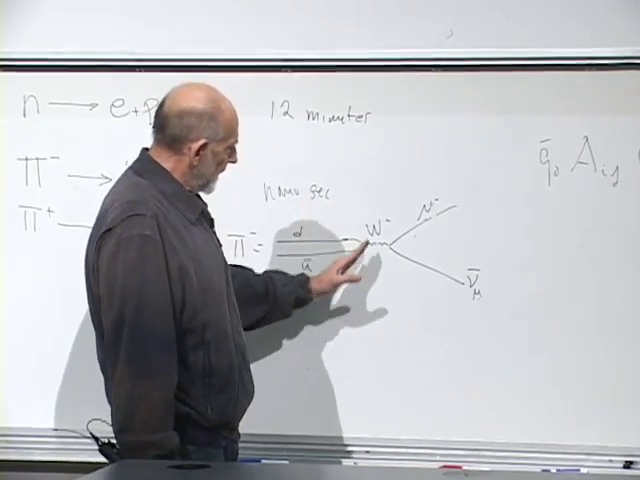
\includegraphics[width=0.72\textwidth]{lecture_05_figure_04.png}\caption{Ein \(d\bar u\)-Pion annihiliert zu einem virtuellen \(W^-\); anschließend entstehen ein geladenes Lepton und das zugehörige Antineutrino.}\lectureframe{01:19:38}\end{figure}

\begin{classroomqa}\audiencequestion{Ist dies wirklich ein Feynman-Diagramm, obwohl die Zeitrichtung horizontal statt vertikal eingezeichnet ist?
\lecturetimestamp{01:20:21}}\lecturerresponse{Ja. Die Orientierung der Zeit auf der Seite ist Konvention. Sobald eine Richtung als Zeit festgelegt und alle Pfeile konsistent interpretiert werden, enthält die Zeichnung dieselbe Information über die Wechselwirkung.}\end{classroomqa}

\begin{classroomqa}\audiencequestion{Kann man das Diagramm eher als umkehrbare chemische Reaktion denn als unumkehrbaren Zerfall lesen?
\lecturetimestamp{01:21:35}}\lecturerresponse{Der umgekehrte Prozess ist erlaubt. Ein im leeren Raum erzeugtes Pion zerfällt, weil sich die austretenden Teilchen voneinander entfernen und gewöhnlich nicht wieder zusammenkommen. Werden jedoch ein Myon und ein Antineutrino mit der passenden Energie und dem passenden Impuls gemeinsam aufeinander geschossen, gibt es eine von null verschiedene Amplitude dafür, dass sie über die umgekehrte Wechselwirkung ein Pion bilden.}\end{classroomqa}

\subsection{Energie und ein virtueller Zwischenzustand}

Für ein ruhendes Pion gilt
\begin{equation}
m_\pi\simeq140\ {\rm MeV},
\qquad
m_\mu\simeq106\ {\rm MeV},
\qquad
m_\nu\approx0
\end{equation}
mit der hier relevanten Genauigkeit. Die verbleibende Energie wird zur kinetischen Energie der austretenden Teilchen. Aus der Impulserhaltung folgt
\begin{equation}
\boldsymbol p_\mu+\boldsymbol p_{\bar\nu}=0,
\end{equation}
Die beiden Teilchen verlassen das Pion-Ruhesystem also in entgegengesetzte Richtungen.

\begin{classroomqa}\audiencequestion{Wie kann die Energie erhalten bleiben, wenn das Zwischen-\(W\) viel schwerer ist als das Pion?
\lecturetimestamp{01:25:08}}\lecturerresponse{Nur die Anfangs- und Endteilchen müssen auf ihrer Massenschale liegen. Der Viererimpuls ist an jedem Vertex erhalten, aber eine interne virtuelle Linie muss \(E^2=\boldsymbol p^2+m_W^2\) nicht erfüllen. Je größer ihre Abweichung von der Massenschale ist, desto stärker unterdrückt ihr Propagator den Prozess.\editorialnote{Die Vorlesung verwendet die traditionelle Sprache der Energie--Zeit-Unschärfe und sagt, der Zwischenzustand könne kurzzeitig die Energie verletzen. Die präzise moderne Aussage ist die in der Antwort: Energie und Impuls sind erhalten, während eine virtuelle interne Linie nicht die Massenschalenbedingung für reale Teilchen erfüllen muss.}}\end{classroomqa}

\subsection{Der Myonzerfall}

Ein Myon kann sich zunächst durch Emission eines virtuellen \(W^-\) in sein eigenes Neutrino umwandeln:
\begin{equation}
\mu^-\longrightarrow\nu_\mu+W^{-*}.
\end{equation}
Das virtuelle Boson erzeugt dann ein Elektron und ein Elektron-Antineutrino:
\begin{equation}
\mu^-\longrightarrow
\nu_\mu+e^-+\bar\nu_e.
\label{eq:l5-muon-decay}
\end{equation}
Dies ist ein rein leptonischer Prozess. Das Myon ist etwa zweihundertmal schwerer als das Elektron, sodass die Ruheenergien der Endteilchen reichlich kinetische Energie übrig lassen.

\begin{figure}[htbp]\centering
\includegraphics[width=0.72\textwidth]{lecture_05_figure_06.png}\caption{Myonzerfall über ein virtuelles geladenes schwaches Boson.}\lectureframe{01:29:24}\end{figure}

\begin{classroomqa}
\audiencequestion{Ist das neutrale Teilchen, das zusammen mit dem Elektron emittiert wird, ein Antineutrino?
\lecturetimestamp{01:29:06}}
\lecturerresponse{Ja. Der vollständige Endzustand enthält ein Myon-Neutrino, ein Elektron-Antineutrino und das Elektron. Anhand der Flavour-Bezeichnungen lassen sich die beiden neutralen Teilchen auseinanderhalten.
}
\end{classroomqa}

Das Elektron kann diesen Zerfall im leeren Raum nicht umkehren, weil es leichter als das Myon ist. Das Tau ist schwerer und kann über analoge schwache Kanäle zerfallen. Die Stabilität ist hier teilweise ein Zufall der Massenordnung und kein Unterschied im zugrunde liegenden Vertex.

\begin{classroomqa}
\audiencequestion{Erhöht ein Linearbeschleuniger effektiv die Masse des Elektrons, sodass andernfalls verbotene Reaktionen in umgekehrter Richtung ablaufen können?
\lecturetimestamp{01:30:23}}
\lecturerresponse{Er ändert nicht die invariante Ruhemasse des Elektrons, sondern stellt kinetische Energie bereit. Eine ausreichend hohe Schwerpunktsenergie kann schwerere Endzustandsteilchen erzeugen. Die zugrunde liegende physikalische Vorstellung stimmt also, wenn man Masse durch die verfügbare Kollisionsenergie ersetzt.
}
\end{classroomqa}

\subsection{Neutronen-Betazerfall auf Quarkebene}

Die Valenzquarkzusammensetzungen von Neutron und Proton sind
\begin{equation}
n=udd,
\qquad
p=uud.
\end{equation}
Ein Down-Quark im Neutron geht über den geladenen Strom in den Übergang
\begin{equation}
d\longrightarrow u+W^{-*},
\end{equation}
wobei \(udd\) in \(uud\) übergeht. Das virtuelle Boson zerfällt anschließend:
\begin{equation}
W^{-*}\longrightarrow e^-+\bar\nu_e.
\end{equation}
Zusammen ergeben die beiden Vertizes
\begin{equation}
n\longrightarrow p+e^-+\bar\nu_e.
\end{equation}

Der umgekehrte Quarkübergang \(u\to d+W^+\) würde ein Baryon aus drei Down-Quarks ergeben. Dieser mögliche Zustand ist jedoch zu schwer, als dass ein freies Neutron ihn erzeugen könnte. Der tatsächliche Übergang von Down zu Up ist energetisch erlaubt.

\begin{classroomqa}
\audiencequestion{Könnte ein Neutron stattdessen in ein Proton, ein Myon und das entsprechende Antineutrino zerfallen?
\lecturetimestamp{01:32:38}}
\lecturerresponse{Nicht bei einem freien Neutron in Ruhe: Die Massendifferenz zwischen Neutron--und Proton ist viel kleiner als die Myonmasse. Mit genügend zusätzlicher Kollisions- oder Anregungsenergie kann derselbe schwache Vertex an einem Kanal beteiligt sein, in dem ein Myon entsteht. Das Verbot ist kinematischer Art und beruht nicht auf einer fehlenden Wechselwirkung.
}
\end{classroomqa}

\section{Die ungeklärte Unterdrückung}

Die geladenen schwachen Vertizes erklären, welche Prozesse stattfinden können, aber noch nicht, warum sie so langsam ablaufen. Eine verlockende Erklärung wäre eine außerordentlich kleine schwache Kopplung. Das ist jedoch falsch: Die dimensionslose schwache Eichkopplung ist ungefähr so groß wie die elektromagnetische. Die Unterdrückung muss also eine andere Ursache haben.

Der fehlende Baustein ist bereits im virtuellen Propagator zu erkennen: Das Boson \(W\) ist sehr massereich. Bei Energien weit unterhalb von \(m_W\) werden die Amplituden geladener Ströme ungefähr durch Potenzen von \(1/m_W^2\) unterdrückt. Dieser Zusammenhang wird später behandelt, nachdem der Higgs-Mechanismus und die elektroschwache Symmetriebrechung erklärt haben, wie die Eichbosonen Masse erhalten.
\editorialnote{Die Vorlesung lässt dieses Rätsel als Frage für die nächste Sitzung offen. Die Erklärung über das schwere \(W\)-Boson ist hier als Ausblick aufgenommen und nicht als Behauptung, dass seine Herleitung in dieser Vorlesung erfolgt sei.}

\begin{classroomqa}
\audiencequestion{Wenn wir sagen, dass die Theorie diese Symmetrie besitzt, meinen wir damit, dass ihre Lagrangefunktion unter den entsprechenden Operationen invariant ist?
\lecturetimestamp{01:34:14}}
\lecturerresponse{Genau. Die Aussage, dass die Theorie die Symmetrie besitzt, ist eine Kurzform dafür, dass die Lagrangefunktion oder gleichwertig die Wirkung unter diesen Transformationen invariant ist. Die vollständige Lagrangefunktion wird auf später verschoben, nicht durch eine andere Definition ersetzt.
}
\end{classroomqa}

Damit ist der Weg vollständig: Die Maxwell-Theorie liefert das Vorbild; die QCD zeigt, wie nichtabelsche Eichbosonen Ladung tragen und austauschen; die Kopplungskonstanten erklären den Unterschied zwischen atomaren und hadronischen Zeitskalen; und die schwache \(SU(2)\)-Symmetrie ordnet Quarks und Leptonen Dubletts zu, die durch \(W^\pm\) miteinander verbunden sind. Es bleibt zu verstehen, warum diese eichvermittelten Prozesse in der Praxis schwach sind, obwohl ihre zugrunde liegende Kopplung nicht außergewöhnlich klein ist.

\chapter{Massiver Austausch schwacher Wechselwirkungen, virtuelle Teilchen und gebrochene Symmetrie}

Die Gruppe des Standardmodells wirkt deutlich weniger rätselhaft, wenn wir sie als Menge zulässiger Bewegungen auf der Fermionentabelle lesen. Farbtransformationen führen vertikal zwischen Rot, Grün und Blau. Geladene schwache Transformationen wirken horizontal innerhalb der Quark- und Lepton-Dubletts. Elektromagnetische Phasentransformationen liefern eine dritte Operation. Die zugehörigen Eichbosonen sind keine nachträglich hinzugefügten Verzierungen der gefundenen Symmetrien: Die Emission eines Eichbosons bewirkt physikalisch dieselbe Zustandsänderung, die ein Erzeuger der Symmetrie beschreibt.

Diese Beobachtung führt zur zentralen Frage dieser Vorlesung. Eine schwache Vertexkopplung ist vergleichbar groß wie eine elektromagnetische, und doch läuft der Betazerfall enorm viel langsamer ab als ein typischer starker oder elektromagnetischer Prozess. Der fehlende Faktor ist die Propagation. Bei kleinem Impuls kostet der Austausch eines massiven \(W\) im Betrag der Amplitude einen Faktor der Größenordnung \(1/m_W^2\). Wir entwickeln diese Aussage zunächst im Ortsraum und dann im Impulsraum, verfolgen ihre Folgen in einer längeren Diskussion realer und virtueller Teilchen und wenden uns schließlich dem ersten qualitativen Modell spontaner Symmetriebrechung zu.

\section{Eichsymmetrie aus der Fermionentabelle ablesen}

\subsection{Farbe wirkt vertikal}

Ordnen wir die sechs Quarkflavours in drei schwache Familien,
\begin{equation}
  (u,d),\qquad(c,s),\qquad(t,b),
\end{equation}
und versehen wir jedes Quark mit einer Farbbezeichnung: Rot, Grün oder Blau. Die entstehende Quarktabelle hat drei Farbzeilen und sechs Flavourspalten. Die Farbe \(SU(3)\) mischt die drei Einträge jeder Flavourspalte. Ein Erzeuger kann beispielsweise ein rotes Up-Quark in ein grünes Up-Quark umwandeln. In der Sprache der Teilchen geht diese Operation mit der Emission eines Gluons einher, das die kompensierende Farbe und Antifarbe trägt.

Dieselbe Farbtransformation muss auf jeden Flavour wirken. Das Gluon, das ein rotes Up-Quark in ein grünes Up-Quark umwandelt, ist dieselbe Gluonenart wie diejenige, die ein rotes Top-Quark in ein grünes Top-Quark umwandelt. Eine echte Symmetrieoperation wirkt auf die erste Generation nicht anders als auf die übrigen. Die Farbänderung erfolgt also vertikal und universell:
\begin{equation}
  q_r\longleftrightarrow q_g\longleftrightarrow q_b,
  \qquad q\in\{u,d,c,s,t,b\}.
\end{equation}
Sie verändert die Farbe, aber nicht den Flavour.

Das ist die charakteristische Beziehung zwischen einer Eichgruppe und ihren Eichbosonen. Die infinitesimalen Erzeuger beschreiben Transformationen zwischen Zuständen; die Emission oder Absorption der entsprechenden Bosonen realisiert diese Transformationen als physikalische Prozesse.

\subsection{Schwache Transformationen wirken horizontal}

Die geladene schwache Wechselwirkung wirkt in die andere Richtung. Ein Quark vom Up-Typ kann ein geladenes schwaches Boson emittieren und so zu seinem Partner vom Down-Typ werden, ohne seine Farbe zu ändern:
\begin{equation}
  u_b\longrightarrow d_b+W^+.
\end{equation}
Genau dieselbe \(W^+\) tritt in
\begin{equation}
  c_g\longrightarrow s_g+W^+,
  \qquad
  t_r\longrightarrow b_r+W^+.
\end{equation}
auf. Die Bezeichnungen \(r,g,b\) bleiben unberührt. Gluonen führen keine horizontalen Änderungen in der Tabelle aus, und geladene \(W\)-Bosonen durchlaufen die Farben nicht vertikal.

Ergänzen wir die elektromagnetische Phasensymmetrie \(U(1)\), unter der jedes geladene Feld eine Phase annimmt. Als erste Näherung ergibt sich dann die Gruppenstruktur
\begin{equation}
  SU(3)\times SU(2)\times U(1).
\end{equation}
Die Kreuzzeichen bedeuten, dass es sich um unabhängige Faktoren handelt: Einer wirkt auf die Farbe, einer auf die schwachen Dubletts und einer durch eine Phase. Das ist ein nützliches grobes Bild, aber noch nicht die vollständige elektroschwache Theorie.\editorialnote{Die Eichgruppe des Standardmodells wird konventionell exakt als \(SU(3)_c\times SU(2)_L\times U(1)_Y\) geschrieben. Die schwache \(SU(2)_L\) wirkt nur auf linkshändige Dubletts, und die endgültige elektromagnetische \(U(1)_{\rm em}\) geht nach der Symmetriebrechung aus \(SU(2)_L\times U(1)_Y\) hervor. Die Vorlesung weist ausdrücklich darauf hin, dass die erste Näherung, in der die letzten beiden Faktoren identifiziert werden, noch nicht vollständig konsistent ist; spätere Vorlesungen ergänzen die fehlende chirale und elektroschwache Struktur.}

\subsection{Dasselbe Muster gilt für Leptonen}

Unterhalb der drei Farbzeilen ordnen wir eine farblose Leptonzeile an:
\begin{equation}
\begin{array}{c|cc|cc|cc}
 &u&d&c&s&t&b\\ \hline
Q&+\frac23&-\frac13&+\frac23&-\frac13&+\frac23&-\frac13\\
\text{lepton partner}
 &\nu_e&e^-&\nu_\mu&\mu^-&\nu_\tau&\tau^-\\
Q&0&-1&0&-1&0&-1
\end{array}
\end{equation}
Innerhalb jedes benachbarten Paars unterscheiden sich die elektrischen Ladungen um eine Einheit. Deshalb kann dasselbe geladene schwache Boson \(u\) mit \(d\), \(c\) mit \(s\), \(t\) mit \(b\) und ein geladenes Lepton mit seinem Neutrino verbinden. Der Vertex des \(W\) hängt von den passenden Quantenzahlen und der Ladungsdifferenz ab, nicht davon, ob das Fermion ein Quark oder ein Lepton ist.

\begin{figure}[htbp]\centering
\includegraphics[width=0.88\textwidth]{lecture_06_figure_07.png}\caption{Die vollständige Fermionentabelle: drei Quark-Farbzeilen oberhalb der farblosen Leptonzeile; die Quarkladungen und die drei Lepton-Dubletts sind zu sehen.}\lectureframe{00:18:55}\end{figure}

Das Myon hat dieselbe Ladung und dieselben bekannten intrinsischen Quantenzahlen wie das Elektron, ist aber etwa zweihundertmal schwerer. Das Tau ist noch schwerer. Die Neutrinomassen sind sehr klein und waren in der Diskussion der Vorlesung nicht im Einzelnen bekannt. Bislang ergibt sich hier kein Prinzip, das das beobachtete Muster der Familienmassen erklärt.

\begin{classroomqa}\audiencequestion{Warum heißen Leptonen, Baryonen und Mesonen so?\lecturetimestamp{00:19:02}}\lecturerresponse{Die historischen griechischen Wortwurzeln bedeuteten ungefähr leicht, schwer und dazwischenliegend. Diese massenbezogene Namensgebung erwies sich als irreführend. Das Myon wurde früher My-Meson genannt, weil seine Masse zwischen der Elektronen- und der Protonenmasse lag; seine Wechselwirkungen zeigen jedoch, dass es ein Lepton ist und einem Elektron viel ähnlicher als einem Pion. Heute bezeichnet Meson ein Hadron aus Quark--Antiquark und ein Boson; das Myon ist kein Meson.}\end{classroomqa}

\section{Das Rätsel der Schwäche}

\subsection{Ein konkreter geladener Stromprozess}

Betrachten wir den Betazerfall des Neutrons als konkretes Diagramm. Die Zusammensetzung aus Valenzquarks lautet
\begin{equation}
  n=udd,\qquad p=uud.
\end{equation}
Ein Down-Quark geht in den Prozess
\begin{equation}
  d\longrightarrow u+W^-,
\end{equation}
über, und das geladene Boson erzeugt
\begin{equation}
  W^-\longrightarrow e^-+\bar\nu_e.
\end{equation}
Zusammen ergibt sich
\begin{equation}
  n\longrightarrow p+e^-+\bar\nu_e.
\end{equation}
Die beiden übrigen Valenzquarks laufen als Zuschauerteilchen weiter. Am ersten Vertex wird aus dem Neutron ein Proton; am zweiten wandelt dieselbe schwache Wechselwirkung, die ein Lepton-Dublett verbindet, das \(W^-\) in das beobachtete Elektron und Elektron-Antineutrino um.

\subsection{Drei Kopplungen, drei sehr unterschiedliche Eindrücke}

In der QED ist die Elektronenladung \(e\) die Vertexamplitude. Ihr Quadrat ergibt die charakteristische Emissionswahrscheinlichkeit; die üblichen Faktoren sind in natürlichen Einheiten in
\begin{equation}
  \alpha=\frac{e^2}{4\pi}\simeq\frac1{137}
\end{equation}
zusammengefasst. Die starke Wechselwirkung hat eine Kopplung \(g_s\), und bei einer typischen hadronischen Energieskala kann ihr Analogon \(\alpha_s\) von der Größenordnung \(0.2\) sein. Das ist viel größer als \(1/137\), deshalb ist die Gluonemission häufig, wenn ein Quark angestoßen wird.

Sei \(g_w\) die Kopplung der geladenen schwachen Wechselwirkung. Ihr Quadrat ist nicht außerordentlich klein; in der hier verwendeten Größenordnungsabschätzung ist es mit der elektromagnetischen Kopplung vergleichbar. Dennoch wartet ein freies Neutron ungefähr fünfzehn Minuten, bevor es zerfällt, während ein starker Zerfall auf einer hadronischen Durchquerungszeit stattfinden kann. Die historische Abschätzung in der Vorlesung verwendet den älteren groben Wert von zwölf Minuten; beide Werte machen das Rätsel gleichermaßen unvermeidlich.\editorialnote{Die moderne mittlere Lebensdauer des freien Neutrons beträgt etwa \(8.8\times10^2\,{\rm s}\); zwischen wichtigen Messmethoden besteht weiterhin eine experimentelle Diskrepanz. Der grobe Wert der Vorlesung dient als pädagogische Größenskala, nicht als Präzisionswert.}
\begin{quote}
Wenn \(g_w\) nicht außerordentlich klein ist, wodurch werden schwache Prozesse dann schwach?
\end{quote}

Die Antwort kann nicht allein bei den Vertizes liegen. Jedes Feynman-Diagramm enthält auch Propagatoren, also Faktoren, die die Zwischenpropagation von einem Vertex zum anderen beschreiben.

\section{Ein massiver Propagator im Ortsraum}

\subsection{Die Vertizes sind nicht das ganze Diagramm}

Das Betazerfallsdiagramm enthält zwei schwache Vertizes, die zwei Potenzen von \(g_w\) beitragen, und eine \(W\)-Linie, die sie verbindet. Bezeichnen wir den Propagator im Ortsraum mit \(\Delta(x-y)\), wobei \(x\) das Emissionsereignis und \(y\) das Absorptions- oder Umwandlungsereignis bezeichnet. Er ist der Amplitudenkern, der zur Übertragung der Feldstörung zwischen diesen Ereignissen gehört.

Der exakte relativistische Propagator enthält mehr Struktur, als wir benötigen. Sein wichtiges qualitatives Merkmal ist seine Massenabhängigkeit. Bei kleinem raumartigem Abstand hat er eine Potenzsingularität, schematisch
\begin{equation}
  \Delta(d)\sim\frac1{d^2}.
\end{equation}
Ein masseloses Feld behält einen Potenzabfall. Ein massives Feld hingegen wird exponentiell unterdrückt, sobald der Abstand groß gegenüber seiner Compton-Skala wird. Die Kurve fällt dann stark ab.

\subsection{Die natürlichen Einheiten bestimmen den Knick}

Setzen wir
\begin{equation}
  c=\hbar=1.
\end{equation}
Dann gilt
\begin{equation}
  [m]=[E]=[p]=L^{-1}.
\end{equation}
Die bekannten Beziehungen erklären die Gleichungen: \(E=mc^2\) setzt Masse und Energie in Beziehung, während \(p\,x\) die Dimension von \(\hbar\) hat, sodass Impuls und Abstand inverse Einheiten besitzen. Die einzige Länge, die sich aus der Masse \(m\) bilden lässt, ist daher
\begin{equation}
  d_m\sim\frac1m.
\end{equation}
Mit wieder eingesetzten Konstanten ergibt sich die Compton-Wellenlänge
\begin{equation}
  d_m\sim\frac{\hbar}{mc},
\end{equation}
Ein schwereres Austauschteilchen hat eine kürzere effektive Reichweite.

\begin{figure}[htbp]\centering
\includegraphics[width=0.78\textwidth]{lecture_06_figure_02.png}\caption{Dimensionen in natürlichen Einheiten und qualitativer Abfall des Propagators. Die schwarze Kurve setzt sich mit einem Potenzabfall fort; die rote Kurve für ein massives Teilchen knickt nahe der inversen Massenskala nach unten ab.}\lectureframe{00:27:19}\end{figure}

\begin{figure}[htbp]\centering
\begin{tikzpicture}[x=1.0cm,y=0.9cm]
  \draw[->] (0,0) -- (7,0) node[right] {$d$};
  \draw[->] (0,0) -- (0,5) node[above] {$|\Delta(d)|$};
  \draw[thick]
    plot[smooth] coordinates {(0.45,4.5) (0.9,3.3) (1.6,2.5)
      (2.5,1.9) (3.7,1.45) (5.1,1.12) (6.4,0.9)};
  \draw[thick,red]
    plot[smooth] coordinates {(0.45,4.5) (0.9,3.3) (1.6,2.5)
      (2.5,1.9) (3.2,1.55) (3.7,0.95) (4.2,0.36) (4.8,0.1)};
  \draw[dashed] (3.4,0) -- (3.4,1.4);
  \node at (5.7,1.4) {$m=0$};
  \node[red] at (4.75,0.72) {$m>0$};
  \node[below] at (3.4,0) {$d\sim m^{-1}$};
\end{tikzpicture}\caption{Eine übersichtliche schematische Darstellung der Argumentation an der Tafel. Sie ist keine exakte Formel für einen vierdimensionalen Propagator, sondern veranschaulicht die durch die Masse bestimmte Reichweite.}\end{figure}

\begin{classroomqa}
\audiencequestion{Was ist auf der vertikalen Achse aufgetragen?
\lecturetimestamp{00:28:30}}
\lecturerresponse{Der Betrag des Propagators, bezeichnet mit \(\Delta\). Sein Quadrat geht in die Wahrscheinlichkeit ein, sobald die vollständige Amplitude, die äußeren Zustände und die Phasenraumfaktoren berücksichtigt werden. Die Abbildung soll zeigen, dass die Amplitude für den Austausch eines massiven Teilchens über große Entfernungen rasch unterdrückt wird.\editorialnote{Ein Propagator für sich genommen ist keine direkt messbare Wahrscheinlichkeitsamplitude für ein Teilchen, das einer klassischen Bahn folgt. Die Formulierung in der Vorlesung liefert eine nützliche Abschätzung der Reichweite: Der Propagator ist ein Faktor in der vollständigen Streuungs- oder Zerfallsamplitude.}}
\end{classroomqa}

\section{Fourier-Transformation und Fermi-Grenzfall}

\subsection{Experimente geben Impulse vor}

Ein Experiment misst gewöhnlich äußere Impulse und nicht die beiden Raumzeitpunkte, an denen eine interne Linie beginnt und endet. Beim Betazerfall wird der vom \(W\) getragene Impuls aus der Differenz zwischen Neutronen- und Protonenimpuls erschlossen und ist gleich dem Gesamtimpuls von Elektron und Antineutrino. Die Propagatoren im Orts- und Impulsraum sind durch eine Fourier-Transformation miteinander verknüpft.
\begin{equation}
  k=p_n-p_p=p_e+p_{\bar\nu_e}.
\end{equation}

In der an der Tafel verwendeten Konvention mit positivem Nenner gilt
\begin{equation}
  \widetilde{\Delta}_W(k)=\frac1{k^2+m_W^2},
  \qquad
  \widetilde{\Delta}_\gamma(k)=\frac1{k^2}.
\end{equation}
Der Propagator des masselosen Photons wird bei kleinem Impulsübertrag groß. Der Propagator des massiven \(W\) überschreitet niemals eine Skala der Größenordnung \(1/m_W^2\). Beim Betazerfall gilt
\begin{equation}
  |k^2|\ll m_W^2,
\end{equation}
Daher sind die Einzelheiten von \(k^2\) vernachlässigbar und
\begin{equation}
  \widetilde{\Delta}_W(k)\simeq\frac1{m_W^2}.
\end{equation}

\begin{classroomqa}\audiencequestion{Müsste der relativistische Ausdruck \(k^2\) ein Minuszeichen zwischen Energie und räumlichem Impuls enthalten?\lecturetimestamp{00:35:11}}\lecturerresponse{Ja. Bei einer Minkowski-Metrik mit Signatur meist minus gilt \(k^2=(k^0)^2-\boldsymbol{k}^2\), und der skalare Nenner lautet konventionell \(k^2-m_W^2+i\epsilon\). Die Tafel verwendet den äquivalenten positiven raumartigen oder euklidischen Betrag. Beim niederenergetischen Betazerfall ist der übertragene Viererimpuls klein gegenüber \(m_W\), sodass beide Schreibweisen dieselbe Unterdrückung um den Faktor \(1/m_W^2\) ergeben, bis auf ein für die Amplitude irrelevantes Vorzeichen.}\end{classroomqa}

\subsection{Die Niederenergie-Amplitude}

Zwei schwache Vertizes und ein Propagator ergeben
\begin{align}
  \mathcal A_{\rm weak}
  &\sim g_w\,\widetilde{\Delta}_W(k)\,g_w\\
  &\sim\frac{g_w^2}{k^2+m_W^2}
  \simeq\frac{g_w^2}{m_W^2}.
\end{align}
Das Quadrieren der Amplitude führt zur charakteristischen Unterdrückung
\begin{equation}
  |\mathcal A_{\rm weak}|^2
  \sim\frac{g_w^4}{m_W^4},
\end{equation}
bevor die für den jeweiligen Zerfall passenden kinematischen und Phasenraumfaktoren berücksichtigt werden. Bei Kernenergien ist die schwache Wechselwirkung nicht deshalb schwach, weil ihre elementare Eichkopplung absurd klein wäre, sondern weil ihr Vermittler schwer ist.

\begin{figure}[htbp]\centering
\includegraphics[width=0.86\textwidth]{lecture_06_figure_03.png}\caption{Der schwache Prozess Neutron--Proton und der vom internen Linienzug getragene Impulsübertrag, wie bei der Klärung des Vorzeichens des Propagators besprochen.}\lectureframe{00:35:40}\end{figure}

\begin{figure}[htbp]\centering
\includegraphics[width=0.84\textwidth]{lecture_06_figure_04.png}\caption{Die Topologie des Betazerfalls neben der eingerahmten Niederenergieabschätzung \(g_w^2/m_W^2\).}\lectureframe{00:37:25}\end{figure}

Numerisch ist \(m_W\) nach der Genauigkeit dieser Vorlesung ungefähr hundert Protonenmassen schwer. Ein Faktor \(m_W^{-2}\) in der Amplitude wird zu \(m_W^{-4}\) in der Zerfallsrate. So führt selbst eine Kopplung von gewöhnlicher Größe in einer Eichtheorie zu einer sehr langen Lebensdauer.

\begin{classroomqa}\audiencequestion{Geht es um eine Unterdrückung um den Faktor eine Million oder eine Milliarde, und wie wurde die Masse des \(W\) ursprünglich bestimmt?\lecturetimestamp{00:38:11}}\lecturerresponse{Die grobe Überschlagsrechnung der Vorlesung deutet auf eine Unterdrückung der Wahrscheinlichkeit bei schwachen Niederenergieprozessen um etwa eine Milliarde gegenüber einem nicht unterdrückten hadronischen Prozess hin. Historisch wurden bei Niederenergieexperimenten \(g_w\) und \(m_W\) nicht getrennt gemessen. Gemessen wurde die kleine Kombination \(g_w^2/m_W^2\), die Fermi-Konstante genannt wird. Nachdem die Kopplung mit der elektroschwachen Theorie verknüpft worden war, sagte diese Kombination einen sehr schweren Vermittler voraus; spätere Beschleuniger erzeugten das \(W\) direkt und bestimmten seine Masse.}\end{classroomqa}

Bei Impulsen weit unterhalb von \(m_W\) sieht jedes Experiment nahezu dieselbe Konstante:
\begin{equation}
  G_F\sim\frac{g_w^2}{m_W^2}.
\end{equation}
Deshalb konnte Fermi den Betazerfall in den 1930er Jahren als punktartige Vier-Fermionen-Wechselwirkung beschreiben, lange bevor der Vermittler beobachtet wurde. Mit steigenden Kollisionsenergien wurden Experimente empfindlich für die im Propagator verborgene Impulsabhängigkeit. So bestätigte sich, dass die effektive Konstante der Niederenergie-Grenzfall eines Austauschs eines massiven Teilchens war.\editorialnote{Bei der üblichen Normierung der elektroschwachen Theorie auf Baumgraphenniveau gilt
\[
  \frac{G_F}{\sqrt2}=\frac{g^2}{8m_W^2}.
\]
Die Vorlesung lässt Zahlen- und Spinorfaktoren bewusst weg und berücksichtigt nur die Skalierung \(G_F\sim g_w^2/m_W^2\). Das \(W\) und das \(Z\) wurden 1983 am CERN direkt entdeckt; die beiläufige Datierung der Vorlesung auf die mittleren bis späten 1970er Jahre liegt vor ihrer direkten Beobachtung.}

Die Vorstellung, dass schwere Teilchen die schwachen Wechselwirkungen vermitteln könnten, kam in der Mitte des zwanzigsten Jahrhunderts auf. Die Vorlesung nennt Julian Schwinger als einen der Theoretiker, die diese Möglichkeit untersuchten, und merkt an, dass der Buchstabe \(W\) wahrscheinlich für „weak“ stand. Niederenergiedaten ließen bereits darauf schließen, dass ein solcher Vermittler auf der Skala der Kernphysik extrem schwer sein müsste – lange bevor Beschleuniger genügend Energie hatten, um ihn als reales Teilchen zu erzeugen.

\subsection{Drei unabhängige Einflussgrößen auf eine Zerfallsrate}

Eine Frage aus dem Unterricht zur Kernbindung unterscheidet drei logisch verschiedene Einflussgrößen auf einen Übergang:
\begin{enumerate}\item Vertexkopplungskonstanten;
\item Propagatoren, einschließlich Massen und Impulsabhängigkeit;
\item verfügbare Energie vom Anfangs- zum Endzustand und Phasenraum.
\end{enumerate}
Bindung kann einen Zerfallskanal schließen, weil der Endzustand eine höhere Energie als der Anfangszustand hätte. Das ist ein kinematisches Verbot, keine zusätzliche Verringerung von \(g_w\) und auch keine Änderung von \(m_W\). Bleibt ein Kanal offen, steht aber nur wenig Energie zur Verfügung, kann sein Phasenraum dennoch stark unterdrückt sein.

\begin{classroomqa}\audiencequestion{Unterdrücken das Feld oder die Bindung eines nahe gelegenen Protons den Betazerfall über denselben Propagatormechanismus?\lecturetimestamp{00:41:13}}\lecturerresponse{Nicht im hier behandelten Beispiel. Die Bindung ist von Bedeutung, weil sie die Energien der Anfangs- und Endzustände des Kerns verändert. Ein Prozess kann nicht stattfinden, wenn der Endzustand energetisch nicht zugänglich ist. Kopplungen, Propagatoren und verfügbare Energie sind drei getrennte Bestandteile.}\end{classroomqa}

\begin{classroomqa}\audiencequestion{Sind die Kopplungskonstanten wirklich konstant?\lecturetimestamp{00:42:55}}\lecturerresponse{Nur bei einer festgelegten Skala. Quantenkorrekturen lassen effektive Kopplungen mit dem Impuls oder dem Abstand laufen. In der vorliegenden Argumentation wird jede Kopplung auf der für den Prozess relevanten Skala betrachtet; die Skalenabhängigkeit wird später behandelt.}\end{classroomqa}

\section{Virtueller Austausch ohne Aufgabe der Erhaltungssätze}

\subsection{Warum die schwere Linie auftreten kann}

Beim gewöhnlichen Neutronenzerfall reicht die Energie nicht aus, um ein freies, reelles \(W\) zu erzeugen. Das \(W\) im Diagramm ist intern und liegt außerhalb der Massenschale. Die Vorlesung führt diesen Sachverhalt mit der traditionellen Energie--Zeit-Abschätzung ein:
\begin{equation}
  \Delta E\,\Delta t\lesssim\hbar:
\end{equation}
Eine Zwischenkonfiguration, deren klassische Energie um \(\Delta E\) falsch zu sein scheint, kann nur während einer Zeitspanne der Größenordnung
\(\hbar/\Delta E\)
beitragen.

Die Analogie zum Tunneleffekt macht das gemeinte Bild anschaulich. Man betrachte ein Alphateilchen in einem Kernpotentialtopf. Seine Energie liegt unterhalb des Barrierenmaximums, sodass es klassisch nicht entkommen kann. Quantenmechanisch reicht die Wellenfunktion durch die Barriere, und das Teilchen kann auf der anderen Seite an einem Punkt mit derselben Gesamtenergie austreten wie anfangs. Versuchen wir, das Innere der Barriere als gewöhnliche klassische Bahn zu beschreiben, scheint die potenzielle Energie zu groß; die kinetische Energie müsste negativ sein. Dieses scheiternde klassische Bild ist vergleichbar mit dem Versuch, die interne Linie \(W\) als reales Teilchen zu betrachten.

\begin{figure}[htbp]\centering
\includegraphics[width=0.78\textwidth]{lecture_06_figure_06.png}\caption{Die Analogie zum Tunneleffekt: Der Anfangspunkt und der markierte Punkt auf der abfallenden Seite haben dieselbe Gesamtenergie, während die dazwischenliegende Barriere klassisch verboten ist.}\lectureframe{00:46:00}\end{figure}

\begin{figure}[htbp]\centering
\begin{tikzpicture}[x=1.0cm,y=0.9cm]
  \draw[->] (0,0) -- (7,0) node[right] {$x$};
  \draw[->] (0,0) -- (0,4.8) node[above] {$V(x)$};
  \draw[thick]
    plot[smooth] coordinates {(0.3,1.4) (1.0,0.7) (1.7,0.55)
      (2.1,0.9) (3.2,3.9) (4.2,2.1) (5.0,0.75) (6.6,0.18)};
  \draw[dashed] (1.7,0.75) -- (5.0,0.75);
  \fill (1.7,0.75) circle (0.06);
  \fill (5.0,0.75) circle (0.06);
  \node at (3.35,0.35) {$\Delta E\,\Delta t\lesssim\hbar$};
\end{tikzpicture}\caption{Eine gut lesbare Rekonstruktion der Barriere und der Punkte gleicher Energie.}\end{figure}

Im Bild des Betazerfalls kann das Neutron in ein Proton und ein internes \(W^-\) fluktuieren, doch die schwere Linie muss rasch enden. Das Boson kann reabsorbiert werden, wodurch das Neutron wiederhergestellt wird, oder die Linie kann am zweiten Vertex enden und das viel leichtere Elektron und Antineutrino erzeugen. Die Gesamtenergien von Anfangs- und Endzustand stimmen überein.\editorialnote{An jedem Feynman-Vertex sind Energie und Impuls erhalten. Virtuelle Teilchen leihen sich nicht buchstäblich Energie, um sie später zurückzuzahlen. Präzise gesagt wird über die Viererimpulse einer internen Linie integriert; diese müssen nicht die Massenschalenbedingung für reale Teilchen erfüllen, \(k^2=m_W^2\). Die Sprache der Unschärferelation und des Tunneleffekts bleibt erhalten, weil sie den Erklärungsweg der Vorlesung bildet; die moderne Formulierung der Quantenfeldtheorie lautet jedoch, dass das Teilchen außerhalb der Massenschale liegt.}

\subsection{Reale W-Bosonen}

Ein hinreichend energiereicher Beschleuniger kann ein reales \(W\) erzeugen. Es hat dann eine eigene Ruhelebensdauer, die nichts mit einer vermuteten Unschärfezeit für die virtuelle Linie zu tun hat. Ein geboostetes reales \(W\) lebt im Labor aufgrund der gewöhnlichen relativistischen Zeitdilatation länger. Beim leptonischen Zweikörperzerfall eines ruhenden \(W\) gilt
\begin{equation}
  W^-\longrightarrow e^-+\bar\nu_e,
\end{equation}
Das Elektron und das Antineutrino tragen große kinetische Energien und fliegen annähernd in entgegengesetzte Richtungen; jede ihrer Energien ist von der Größenordnung \(m_W/2\). Die Ruheenergie ist nicht verschwunden, sondern in Energie des Endzustands übergegangen. Auch Myon- und Taukanäle sowie Quarkkanäle sind möglich.

\begin{classroomqa}
\audiencequestion{Wie lange lebt ein reales \(W\), und lässt sich seine Lebensdauer aus derselben Kopplung berechnen?
\lecturetimestamp{00:49:49}}
\lecturerresponse{Ja. Man berechnet jede erlaubte Zerfallsamplitude, quadriert sie, integriert über den Phasenraum der Endzustände und summiert die partiellen Zerfallsbreiten. Die inverse Gesamtbreite ergibt die Lebensdauer. Die gesprochene numerische Schätzung im Transkript ist verstümmelt; der qualitative Punkt ist jedoch, dass die Eigenlebensdauer extrem kurz ist und sich bei einem bewegten \(W\) wie üblich durch Zeitdilatation verlängert.\editorialnote{Mit der gemessenen Breite
\(\Gamma_W\simeq2.1\,{\rm GeV}\) ergibt sich
\(\tau_W=\hbar/\Gamma_W\simeq3.2\times10^{-25}\,{\rm s}\). Diese moderne Zahl bringt Klarheit in den entstellten Zahlenaustausch, ohne sie der Vorlesung zuzuschreiben.}}
\end{classroomqa}

\begin{classroomqa}\audiencequestion{Wie wird aus einer quadrierten Amplitude eine Zerfallsrate und damit eine Lebensdauer?\lecturetimestamp{00:50:52}}\lecturerresponse{Das quadrierte Matrixelement wird mit der Dichte der verfügbaren Endzustände, Erhaltungs-Deltafunktionen und Normierungsfaktoren kombiniert. So erhält man eine Übergangswahrscheinlichkeit pro Zeiteinheit, die Zerfallsbreite \(\Gamma\). Die Überlebenswahrscheinlichkeit lautet \(e^{-\Gamma t}\) in Einheiten mit \(\hbar=1\), also \(\tau=1/\Gamma\) oder mit wieder eingesetzten Einheiten \(\tau=\hbar/\Gamma\). Eine kleine schwache Zerfallsbreite bedeutet daher eine lange Lebensdauer.}\end{classroomqa}

\begin{classroomqa}\audiencequestion{Kann man einem Teilchen, das durch die Barriere tunnelt, eine Geschwindigkeit zuordnen?\lecturetimestamp{00:52:42}}\lecturerresponse{Man kann eine erschlossene Entfernung durch eine erschlossene Durchquerungszeit teilen, doch diese Größe sollte nicht als Geschwindigkeit eines klassischen Teilchens oder eines Signals gedeutet werden. Der Versuch, eine Bahn im Inneren der Barriere zu messen, verändert den Zustand und zerstört das ursprüngliche Tunnelexperiment.}\end{classroomqa}

\section{Was bedeutet es, ein virtuelles Teilchen zu beobachten?}

\subsection{Äußere Teilchen und interne Linien}

Reale Teilchen sind einlaufende und auslaufende asymptotische Zustände, die sich weit entfernt vom Wechselwirkungsgebiet präparieren oder nachweisen lassen. Virtuelle Teilchen sind interne Linien in einer störungstheoretischen Darstellung der Amplitude. Sie sind keine zusätzlichen, verborgenen Spuren im Detektor.

\begin{classroomqa}\audiencequestion{Gibt es eine klare Definition des Unterschieds zwischen einem realen und einem virtuellen Teilchen?\lecturetimestamp{00:55:05}}\lecturerresponse{Ein reales Teilchen ist ein äußerer Zustand auf der Massenschale, der in das Wechselwirkungsgebiet eintritt oder es verlässt. Ein virtuelles Teilchen ist eine interne Linie außerhalb der Massenschale in einem Feynman-Diagramm. Letztere ist Teil der mathematischen Entwicklung und kein unabhängig beobachtetes Objekt.}\end{classroomqa}

Um einen Prozess aufzulösen, der nur \(\Delta t\) dauert, benötigt eine Sonde Frequenzen der Größenordnung \(1/\Delta t\) und damit eine Energie der Größenordnung \(\hbar/\Delta t\). Ein Photon, dessen Auflösung ausreicht, um ein Alphateilchen unter einer hohen Barriere sichtbar zu machen, kann ihm die Energie zuführen, die es in den Barrierenbereich hebt. Ebenso kann eine Sonde, die energiereich genug ist, um die kurzlebige interne Linie \(W\) aufzulösen, ein reales \(W\) erzeugen. Der Beobachtungsversuch macht aus dem ursprünglichen Prozess ein anderes Experiment.

Die Vorlesung beschreibt dies als wiederkehrende quantenmechanische Frustration: Der Eingriff, der nötig ist, um das verbotene Zwischenbild zu überprüfen, liefert gerade die Energie, durch die die scheinbar verbotene Konfiguration real wird.

\subsection{Fluktuationen eines Protons}

In der Störungstheorie enthält ein Protonenzustand Amplituden für Konfigurationen wie
\begin{equation}
  p\longleftrightarrow n+W^+,
\end{equation}
und ein Neutron entsprechend
\begin{equation}
  n\longleftrightarrow p+W^-.
\end{equation}
Greift keine andere Wechselwirkung ein, wird das interne Boson reabsorbiert. Eine harte Sonde kann stattdessen ein \(W\) unter den auslaufenden Teilchen zurücklassen. Man kann das als Herausschlagen einer Fluktuation oder als Erzeugung eines \(W\) bezeichnen. Die Formulierung ist unterschiedlich; die messbare Aussage über die Amplitude des Endzustands ist dieselbe.

\begin{classroomqa}\audiencequestion{Wenn eine harte Sonde ein auslaufendes \(W\) erzeugt, hat sie dann ein bereits vorhandenes Teilchen herausgeschlagen oder ein neues erzeugt?\lecturetimestamp{01:01:20}}\lecturerresponse{Beide Bilder können die mathematische Beschreibung strukturieren. Eine zeitgeordnete Beschreibung besagt, dass das Proton zu \(n+W^+\) fluktuierte und die Sonde das Neutron vor der Reabsorption entfernte; eine andere besagt, dass die Kollision das Endzustands-\(W\) erzeugte. Invariant ist die berechnete Wahrscheinlichkeit für den beobachteten Endzustand, nicht eine eindeutige klassische Erzählung darüber, was vor der Messung vorhanden war.}\end{classroomqa}

Eine Erhöhung der Kollisionsenergie legt keinen festen Bestand von Objekten frei, die zuvor im Target verborgen waren. Sie eröffnet zahlreiche mögliche Endzustände: ein \(W\), mehrere Bosonen, Quarkjets, Hadronen und andere Teilchen, die mit den Erhaltungsbedingungen der Quantenzahlen vereinbar sind. Selbst ein elementares Feld kann bei hinreichend heftigem Stoß Protonen und viele andere zusammengesetzte Objekte hervorbringen. Was herauskommt, muss nicht zuvor als Bestandteil vorhanden gewesen sein. Die Vorlesung treibt den Gedanken bis ins Komische: Wenn Energie und Quantenzahlen es zulassen, sind selbst Tische, Stühle oder ein Wasserstoffatom als geradezu fantastikwahrscheinliche Endanordnungen logisch nicht ausgeschlossen. Der Scherz enthält eine ernsthafte Warnung davor, Elementarität durch eine naive Bestandsaufnahme der Kollisionsprodukte zu definieren.

\subsection{Vakuumfluktuationen und Temperatur}

Eine Fluktuation, die mit einem Proton verbunden ist, ist nicht dasselbe wie ein Vakuumdiagramm. Erstere ist Bestandteil eines wechselwirkenden Protonenzustands; eine Vakuumfluktuation hat keine äußere Protonenlinie. In beiden Fällen kann eine hinreichend energiereiche Sonde reale Teilchen erzeugen, die einem erlaubten Endzustand entsprechen. Zwei energiereiche Photonen können beispielsweise ein Elektron--Positron-Paar erzeugen, wenn die Schwerpunktsenergie über der Schwelle liegt.

\begin{classroomqa}
\audiencequestion{Sind diese Reaktionen temperaturabhängig?
\lecturetimestamp{01:05:17}}
\lecturerresponse{Die elementare Amplitude erfordert kein Wärmebad.
Die Temperatur ist statistisch von Bedeutung: Ein System mit hoher Temperatur enthält viele
Teilchen mit hoher kinetischer Energie, sodass Stöße, bei denen die Schwelle überschritten wird, häufig werden.
Die Erwärmung eines Systems mit einem gebundenen Alphateilchen kann zusätzlich zum Quantentunneln auch
genügend Energie für einen Austritt über die Barriere liefern.
Einige wenige isolierte energiereiche Teilchen bilden einen Strahl; viele thermisch
verteilte energiereiche Teilchen bilden ein heißes Wärmebad.}
\end{classroomqa}

\begin{classroomqa}
\audiencequestion{Ist das \(W\), das bei einer Fluktuation des Protons emittiert wird, eine Vakuumfluktuation?
\lecturetimestamp{01:06:56}}
\lecturerresponse{Nein. Das interne \(W\) in
\(p\leftrightarrow n+W^+\) ist eine Fluktuation des wechselwirkenden Protonzustands.
Ein abgeschlossener virtueller Prozess ohne äußeres Proton ist eine Vakuumfluktuation.
Beide folgen denselben Regeln der Feldtheorie, gehören aber zu unterschiedlichen Amplituden.}
\end{classroomqa}

\begin{classroomqa}
\audiencequestion{Warum ist das Antineutrino am leptonischen \(W\)-Vertex erforderlich?
\lecturetimestamp{01:08:51}}
\lecturerresponse{Es trägt die erhaltenen Leptonenquantenzahlen bei und ist Teil des grundlegenden geladenen Stromvertices, das \(e\), \(\nu_e\) und \(W\) verbindet.
Der Überstrich unterscheidet das auslaufende Elektron-Antineutrino von einem Neutrino.}
\end{classroomqa}

\section{Wie weit lässt sich die Energieumwandlung treiben?}

Die Vorlesung treibt nun die Regel, dass Energie Teilchen erzeugen kann, absichtlich bis ins Absurde. Könnte aus einer Kaffeebohne ein Schokoladenkuchen werden?
Einen praktikablen Prozess dieser Art gibt es nicht, doch die relativistische Quantentheorie schreibt nicht vor, dass die Endmaterie dem anfänglichen Objekt ähneln muss. Erforderlich sind genügend Energie, die richtigen erhaltenen Ladungen und eine von null verschiedene Amplitude. Ein Kilogramm entspricht einer Energie in der Größenordnung von
\begin{equation}
  Mc^2\sim9\times10^{16}\ {\rm J},
\end{equation}
sodass jeder mikroskopische Stoß, der ein bestimmtes Objekt von der Masse eines Kilogramms zusammensetzen würde, unvorstellbar unwahrscheinlich wäre.

Die Planck-Masse,
\begin{equation}
  m_{\rm P}=\sqrt{\frac{\hbar c}{G}}
  \simeq2.2\times10^{-5}\ {\rm g},
\end{equation}
ist keine maximal mögliche Masse. Sie ist die Skala, bei der die Gravitation für ein Quant stark wird, das auf seine Compton-Wellenlänge lokalisiert ist. Ein Kilogramm enthält ungefähr \(5\times10^7\) Planck-Massen.

\begin{classroomqa}
\audiencequestion{Können bei Stößen oberhalb der Planck-Skala beliebig schwere Objekte wie Stühle oder Planeten entstehen?
\lecturetimestamp{01:10:37}}
\lecturerresponse{Bei transplanckscher Schwerpunktsenergie, die auf einen kleinen Raumbereich konzentriert ist, ist der Gravitationskollaps das mit Abstand naheliegendste Ergebnis: ein Schwarzes Loch. Ein stark geordnetes makroskopisches Objekt wäre eine außerordentlich seltene Fluktuation. Die Vorlesung beruft sich auf die Zeitumkehr: Da ein Stuhl in ein Schwarzes Loch fallen kann, ist die umgekehrte Amplitude nicht exakt null. Ihre Wahrscheinlichkeit wird durch einen enormen Entropiefaktor unterdrückt; Möglichkeit darf also nicht mit praktischer Wahrscheinlichkeit verwechselt werden.}
\end{classroomqa}

Dieser Exkurs bekräftigt die frühere Warnung. Die Quantenfeldtheorie sagt Amplituden zwischen festgelegten Anfangs- und Endzuständen voraus. Die anschauliche Behauptung, jedes Produkt sei vor dem Aufprall buchstäblich im Ziel enthalten gewesen, gehört nicht zur Vorhersage.

\section{Bosonen, ihre Wechselwirkungen und ihre Statistik}

\subsection{Photonen können streuen}

Ein Boson zu sein bedeutet nicht, wechselwirkungsfrei zu sein. Die Bezeichnungen Boson und Fermion legen die Austauschstatistik fest; Wechselwirkungsvertices sind davon unabhängige dynamische Eigenschaften.
Klassische Lichtstrahlen durchdringen einander normalerweise, weil es in der QED auf Baumebene kein Vier-Photonen-Vertex gibt und die Streuung von Photonen--Photonen bei niedrigen Energien äußerst gering ist. Dennoch können zwei Photonen über eine virtuelle Elektron--Positron-Schleife wechselwirken:
\begin{equation}
  \gamma+\gamma
  \longrightarrow(e^-e^+)_{\rm virtual}
  \longrightarrow\gamma+\gamma.
\end{equation}
Ist die Schwerpunktsenergie hoch genug, können sie stattdessen ein reelles Paar erzeugen,
\begin{equation}
  \gamma+\gamma\longrightarrow e^-+e^+.
\end{equation}
Optische Photonen haben Energien von einigen Elektronenvolt, während die Paarbildungsschwelle in der Größenordnung von \(2m_e c^2\approx1.02\,{\rm MeV}\) liegt. Der virtuelle Prozess ist bei gewöhnlichen optischen Energien daher stark unterdrückt. Deshalb scheinen sich kreuzende Lichtstrahlen nicht gegenseitig zu beeinflussen.

\begin{classroomqa}
\audiencequestion{Wechselwirken virtuelle \(W\)-Bosonen mit anderen Bosonen einfach deshalb, weil sie Bosonen sind?
\lecturetimestamp{01:12:47}}
\lecturerresponse{Sie können wechselwirken, aber nicht allein deshalb, weil sie der Bose-Statistik folgen. Die Eichvertices legen die dynamischen Wechselwirkungen fest. Die Statistik bestimmt hingegen, wie sich Mehrteilchenamplituden beim Austausch identischer Teilchen verhalten. Photonen wechselwirken schwach über geladene virtuelle Teilchen; außerdem enthält die elektroschwache Theorie direkte nichtabelsche Selbstwechselwirkungen von \(W\)-Bosonen.}
\end{classroomqa}

\subsection{Bose-Verstärkung ist keine Kraft}

Der Unterschied zwischen Fermionen- und Bosonenstatistik tritt deutlich zutage, wenn sich mehrere identische Teilchen in nahe beieinanderliegenden Quantenzuständen befinden. Bosonen begünstigen die Mehrfachbesetzung; Fermionen schließen eine identische Besetzung aus. Bei einer typischen hochenergetischen Kollision bewegen sich die Teilchen in gut getrennte Impulszustände, sodass dieser statistische Effekt weniger auffällig sein kann als bei einem Laser oder einem Kondensat.

Grundsätzlich unterliegen \(W\)-Bosonen derselben Bose-Verstärkung. Die Vorlesung scherzt, man könne sich ein System vorstellen, das \(W\)-Bosonen lasert. Ihre enorme Masse und extrem kurze Lebensdauer machen ein solches Gerät völlig unpraktikabel, doch ihre Statistik ist tatsächlich bosonisch.

\begin{classroomqa}
\audiencequestion{Welche Farbe hat ein Proton oder Neutron?
\lecturetimestamp{01:18:41}}
\lecturerresponse{Ein physikalisches Hadron ist ein Farbsingulett und wird oft als farblos oder weiß bezeichnet. Die Kurzform besagt, dass ein Baryon ein rotes, ein grünes und ein blaues Quark enthält. Genauer gesagt ist seine Farbwellenfunktion die antisymmetrische Superposition
\[
  |{\rm singlet}\rangle
  =\frac1{\sqrt6}\epsilon_{abc}|q^a q^b q^c\rangle,
\]
und keine klassische Zuordnung einer festen Farbe zu jedem namentlich bezeichneten Quark.}
\end{classroomqa}

\begin{classroomqa}
\audiencequestion{Wird Bose-Kondensation in dieser Vorlesung behandelt?
\lecturetimestamp{01:19:25}}
\lecturerresponse{Ja, im Zusammenhang mit dem Higgs-Phänomen. Ein überall im Vakuum von null verschiedenes Higgs-Feld ist in wichtigen Aspekten einem bosonischen Kondensat ähnlich. Die Analogie wird erläutert, nachdem die spontane Symmetriebrechung eingeführt worden ist.\editorialnote{Der Vakuumerwartungswert des Higgs-Feldes ist nicht wörtlich ein gewöhnliches Gas aus auf der Massenschale liegenden Higgs-Teilchen, die denselben Zustand besetzen. Die Kondensation ist eine aufschlussreiche Analogie für ein kohärentes bosonisches Feld und ein ausgewähltes Vakuum, aber keine vollständige mikroskopische Identifikation.}}
\end{classroomqa}

\section{Das fehlende neutrale schwache Boson}

Kehren wir nun zur Gruppentabelle zurück. Ist die horizontale schwache Symmetrie \(SU(2)\), so hat sie
\begin{equation}
  \dim SU(2)=3
\end{equation}
Generatoren und damit drei Eichfelder. Die geladenen Kombinationen \(W^+\) und \(W^-\) entsprechen nur zwei davon. Ein drittes, neutrales Feld ist erforderlich.
Es ist eng mit dem beobachteten \(Z\)-Boson verwandt, aber nicht einfach das Photon. Die genauen neutralen Kombinationen umfassen sowohl das dritte \(SU(2)_L\)-Feld als auch das \(U(1)_Y\)-Feld. Diese Mischung und die korrekte Definition der elektrischen Ladung werden bewusst auf die nächste Vorlesung verschoben.

\section{Spontane Symmetriebrechung}

\subsection{Eine symmetrische Wahl kann instabiles Schwanken hervorbringen}

Stellen wir uns einen runden Esstisch vor, an jedem Platz liegt links und rechts je ein Besteckteil. Bevor sich jemand bewegt, sind links und rechts gleichwertig. Sobald ein Gast nach rechts greift, ist jede benachbarte Wahl festgelegt, und der ganze Tisch ordnet sich rechtsherum an. Die Regeln waren symmetrisch, doch die tatsächlich verwirklichte Konfiguration wählte eine von zwei Möglichkeiten. Die Geschichte ist nur eine Analogie, veranschaulicht aber genau die Kombination, die wir benötigen: Symmetrie, mehrere gleichwertige Ergebnisse und eine Instabilität, durch die eine beliebig kleine Störung global eines davon auswählt.

\subsection{Das Kopf--Zahl-Gitter}

Betrachten wir als einfacheres Modell ein Gitter mit einer Zwei-Zustands-Variablen \(s_i=\pm1\) an jedem Gitterplatz. Nennen wir \(+1\) Kopf und \(-1\) Zahl. Benachbarte Gitterplätze sollen bevorzugt gleich ausgerichtet sein:
\begin{equation}
  H=-J\sum_{\langle ij\rangle}s_i s_j,
  \qquad J>0.
\end{equation}
Parallele Nachbarn tragen weniger zur Energie bei als antiparallele. Daher gibt es zwei entartete Grundzustände,
\begin{equation}
\begin{aligned}
  s_i&=+1\quad\text{for every }i,
  \\
  s_i&=-1\quad\text{for every }i.
\end{aligned}
\end{equation}
Der Hamiltonoperator ist unter der globalen Umkehrung \(s_i\to-s_i\) invariant, doch keiner der beiden ausgewählten Grundzustände ist es.

Fixieren wir nun einen sehr weit entfernten Randspin auf Kopf. In einem gewöhnlichen System mit kurzreichweitigen Wechselwirkungen könnte man erwarten, dass ein einzelner, weit entfernter Freiheitsgrad hier keinen Einfluss hat. In der geordneten Phase wählt diese Randbedingung jedoch das Vakuum mit lauter Kopfzuständen aus. Ist es einmal ausgewählt, kostet ein einzelner Zahlzustand im Meer von Kopfzuständen Energie, weil er nicht mit seinen Nachbarn übereinstimmt. Lokale Anregungen werden relativ zum ausgewählten Grundzustand definiert, obwohl die zugrunde liegenden Gleichungen die Kopf--Zahl-Symmetrie bewahren.

\subsection{Explizite Symmetriebrechung und Domänenwände}

Bei expliziter Symmetriebrechung würde ein lokaler Bias hinzugefügt:
\begin{equation}
  H_{\rm explicit}
  =-J\sum_{\langle ij\rangle}s_i s_j-h\sum_i s_i,
  \qquad h\ne0.
\end{equation}
Dann haben Kopf und Zahl bereits an einem einzelnen Gitterplatz unterschiedliche Energien, und es gibt nur ein bevorzugtes Vakuum. Bei spontaner Symmetriebrechung gilt \(h=0\): Die lokalen Regeln sind symmetrisch, und die beiden Vakua bleiben entartet, aber das System befindet sich in einem davon.

Nehmen wir stattdessen an, der äußerste linke Rand bestehe ganz aus Kopfzuständen und der äußerste rechte ganz aus Zahlzuständen. Die Konfiguration niedrigster Energie muss zwischen den beiden Vakua übergehen. Die Grenzfläche ist eine Domänenwand.

\begin{figure}[htbp]\centering
\includegraphics[width=0.9\textwidth]{lecture_06_figure_08.png}\caption{Das Kopf--Zahl-Gitter, geteilt durch eine gestrichelte Domänenwand. Entgegengesetzte Randbedingungen zwingen das System, eine Grenzfläche zwischen den beiden entarteten geordneten Zuständen zu enthalten.}
\lectureframe{01:30:35}
\end{figure}

\begin{classroomqa}
\audiencequestion{Worin unterscheidet sich spontane Symmetriebrechung von gewöhnlicher expliziter Symmetriebrechung?
\lecturetimestamp{01:28:36}}
\lecturerresponse{Bei expliziter Symmetriebrechung weist der lokale Hamiltonoperator Kopf und Zahl bereits unterschiedliche Energien zu; daher gibt es kein Paar symmetrieverwandter Grundzustände. Bei spontaner Symmetriebrechung bleibt die Symmetrie in den Gleichungen erhalten, die Vakua sind entartet, und Randbedingungen oder eine beliebig kleine Störung wählen eines davon aus. Dass eine Domänenwand zwischen verschiedenen Vakua möglich ist, ist ein Kennzeichen der spontanen Symmetriebrechung.}
\end{classroomqa}

Das Modell ist bewusst äußerst einfach, enthält aber die wesentliche Logik, die wir auf das Higgs-Feld übertragen werden: eine symmetrische Theorie, eine instabile oder entartete Vakuumstruktur, einen ausgewählten Grundzustand und physikalische Konsequenzen, die durch diese Wahl bestimmt werden.

\section{Was diese Vorlesung offenlässt}

Die Fermionentabelle übersetzt die Gruppe des Standardmodells in physikalische Richtungen. Die Farbe \(SU(3)\) bewegt sich vertikal durch Rot, Grün und Blau; geladene schwache Transformationen bewegen sich horizontal durch Quark- und Lepton-Dubletts; eine Phasensymmetrie liefert den vorläufigen Faktor \(U(1)\). Die Emission von Eichbosonen realisiert diese Gruppentransformationen als Wechselwirkungen.

Die Schwäche des Betazerfalls wird damit nicht auf ein außergewöhnlich kleines \(g_w\) zurückgeführt, sondern auf den schweren Vermittler. Im Ortsraum schneidet die Masse den Propagator jenseits der Compton-Skala \(\hbar/(m_Wc)\) ab. Im Impulsraum gilt bei Kernimpulsen
\begin{equation}
  \mathcal A_{\rm weak}
  \sim\frac{g_w^2}{k^2+m_W^2}
  \simeq\frac{g_w^2}{m_W^2}
\end{equation}
Alte Niederenergieexperimente maßen diese Kombination als Fermi-Konstante.

Die ausführliche Diskussion im Hörsaal verdeutlicht, was diese Formel bedeutet und was nicht. Interne \(W\)-Linien sind virtuell und nicht auf der Massenschale; Energie--Impuls bleibt dennoch erhalten. Eine ausreichend energiereiche Sonde kann ein reelles \(W\) erzeugen, doch dann hat sie einen anderen Endzustandsprozess hervorgerufen. Stoßprodukte sind keine wörtliche Liste bereits vorhandener Bestandteile. Die Temperatur verändert die Anzahl energiereicher Geschosse, Photonen können über geladene virtuelle Teilchen wechselwirken, und die Bose-Statistik ist von einer dynamischen Kraft zu unterscheiden.

Schließlich erfordert \(SU(2)\) ein fehlendes neutrales Eichfeld, das mit dem \(Z\) verwandt ist, und das Kopf--Zahl-Gitter liefert das erste Modell der spontanen Symmetriebrechung. Als Nächstes führen wir diese beiden noch offenen Themen zusammen: die elektroschwache Mischung und den Higgs-Mechanismus.

\chapter{Gebrochene Symmetrie, Goldstone-Bosonen und Eichinvarianz}

Wir wollen verstehen, wie ein photonartiges Teilchen eine Masse erhalten kann. Das ist das Ziel, aber kein sinnvoller Ausgangspunkt. Ein direkter Massenterm für ein Eichfeld scheint gerade jene Eichinvarianz zu zerstören, die die Konsistenz der Theorie gewährleistet. Bevor wir den Ausweg erkennen können, müssen wir zwei Ideen in ihrer konkreten Form verstehen:
\begin{enumerate}
  \item spontane Symmetriebrechung, insbesondere bei einer kontinuierlichen Symmetrie;
  \item Eichinvarianz, bei der die Symmetrieoperation von einem Raumzeitpunkt zum anderen variieren darf.
\end{enumerate}
Keine der beiden Ideen lässt sich durch einen bloßen Merksatz ersetzen. Wir entwickeln die erste anhand eines Magneten, übertragen sie auf die Theorie skalarer Felder und entdecken den masselosen Goldstone-Modus. Dann machen wir dieselbe \(U(1)\)-Symmetrie lokal, was uns zwingt, ein Vektorpotential und eine kovariante Ableitung einzuführen. Erst am Ende stellen wir die beiden Gedankengänge nebeneinander. Ihre tatsächliche Verbindung---das Higgs-Phänomen---ist Thema der nächsten Vorlesung.

\section{Ein symmetrisches Gesetz mit einem asymmetrischen Grundzustand}

\subsection{Der Zweizustandsmagnet}

Betrachten wir ein Gitter aus kleinen Magneten. Jeder Spin kann nach oben oder unten zeigen, und benachbarte Spins haben eine geringere Energie, wenn sie in dieselbe Richtung zeigen. Auf einem dreidimensionalen kubischen Gitter hat ein Spin sechs nächste Nachbarn, doch die genaue Koordinationszahl ist unwichtig. Entscheidend ist die Regel
\begin{equation}
  E_{\parallel}<E_{\rm antiparallel}.
\end{equation}
Die mikroskopische Regel bleibt unverändert, wenn alle Spins umgekehrt werden:
\begin{equation}
  \uparrow\longleftrightarrow\downarrow.
\end{equation}
Dennoch sind die Konfigurationen niedrigster Energie nicht jeweils für sich symmetrisch. Sie lauten
\begin{equation}
  \{\uparrow\uparrow\uparrow\cdots\},
  \qquad
  \{\downarrow\downarrow\downarrow\cdots\}.
\end{equation}
Die Gleichungen erlauben beide, doch eine kalte makroskopische Probe muss sich für eine davon entscheiden.

Diese Wahl ist außerordentlich empfindlich. Wir fixieren einen sehr weit entfernten Spin so, dass er nach oben zeigt. Seine Nachbarn richten sich bevorzugt nach ihm aus, deren Nachbarn wiederum nach ihnen, und die Information breitet sich durch die Probe aus. Eine Störung, die im Vergleich zum Gesamtsystem beliebig klein ist, kann die Orientierung des gesamten Grundzustands festlegen. Das ist die Instabilität, die mit \emph{spontan}er Symmetriebrechung gemeint ist.

\begin{classroomqa}
\audiencequestion{Kann ein neutrales Teilchen sich in einem Magnetfeld ausrichten?
\lecturetimestamp{00:05:14}}
\lecturerresponse{Ja. Elektrische Neutralität bedeutet nicht, dass kein magnetisches Moment vorhanden ist. Das Neutron ist neutral, besitzt aber aufgrund seiner inneren geladenen Bestandteile ein magnetisches Moment. Ein Magnetfeld kann daher zwischen seinen Spinorientierungen unterscheiden.}
\end{classroomqa}

\begin{classroomqa}
\audiencequestion{Wenn das System seine Orientierung ändert, geschieht das dann überall gleichzeitig? Können mehrere Umorientierungswellen nebeneinander bestehen?
\lecturetimestamp{00:05:41--00:06:38}}
\lecturerresponse{Die Änderung breitet sich aus. Ein Bereich kippt seine Nachbarbereiche, ähnlich wie bei einem dreidimensionalen Dominofeld, und die Störung wandert als Welle weiter. Verschiedene Bereiche können unabhängig voneinander mit ihrer Wahl beginnen, sodass mehrere Fronten und mehrere Domänen vorhanden sein können, bevor sich eine Orientierung durchsetzt. Auf genau diese Wellen kommen wir zurück, wenn die Symmetrie kontinuierlich wird.}
\end{classroomqa}

\subsection{Explizite Brechung ist eine andere Theorie}

Bringen wir die Probe nun in ein externes, nach oben gerichtetes Magnetfeld. Ein isolierter Spin hat bereits eine niedrigere Energie, wenn er nach oben zeigt. Die Transformation \(\uparrow\leftrightarrow\downarrow\) lässt die Energie nicht länger unverändert: Die Bevorzugung ist in das Gesetz selbst eingebaut. Das ist \emph{explizite}Symmetriebrechung.

Der Unterschied lässt sich prüfen, ohne zu wissen, wie die Probe präpariert wurde. Wir nehmen eine sehr große Probe, halten ihren linken Rand nach oben und ihren rechten Rand nach unten. Bevorzugt ein magnetisches Bulk-Feld explizit die Ausrichtung nach oben, dringt die Randbedingung am rechten Ende nur ein kurzes Stück weit ein. Eine makroskopische Region mit Ausrichtung nach unten würde eine Energie kosten, die proportional zu ihrem Volumen ist; das Bulk kann daher nicht in zwei gleichwertige Phasen unterteilt bleiben.

Ohne äußere Bevorzugung haben die Ausrichtungen nach oben und nach unten dieselbe Bulk-Energie. Der Zustand niedrigster Energie unter den Randbedingungen enthält dann eine Domäne mit Ausrichtung nach oben, eine mit Ausrichtung nach unten und eine endliche Übergangsschicht dazwischen. Die Grenzfläche muss nicht genau in der geometrischen Mitte liegen, doch es gibt keinen Volumendruck, der eine Phase dazu zwingt, die andere zu beseitigen. Diese Grenzfläche ist eine \emph{Domänenwand}, die charakteristische Defektstruktur dieser gebrochenen diskreten Symmetrie.

\begin{figure}[htbp]
\centering
\begin{adjustbox}{max width=\linewidth}
\begin{tikzpicture}[x=0.86cm,y=0.78cm]
  \draw[thick] (0,0) rectangle (11,4);
  \fill[blue!8] (0,0) rectangle (5.15,4);
  \fill[orange!10] (5.85,0) rectangle (11,4);
  \fill[gray!18] (5.15,0) rectangle (5.85,4);
  \foreach \x in {0.7,1.7,2.7,3.7,4.7}
    \foreach \y in {0.65,1.65,2.65,3.65}
      \node[blue!65!black] at (\x,\y) {$\uparrow$};
  \foreach \x in {6.3,7.3,8.3,9.3,10.3}
    \foreach \y in {0.65,1.65,2.65,3.65}
      \node[orange!65!black] at (\x,\y) {$\downarrow$};
  \draw[dashed,thick] (5.5,0) -- (5.5,4);
  \node[above] at (2.6,4) {up vacuum};
  \node[above] at (8.45,4) {down vacuum};
  \node[rotate=90,fill=white,inner sep=2pt] at (5.5,2) {domain wall};
  \node[left,align=right] at (0,2) {boundary\\fixed up};
  \node[right,align=left] at (11,2) {boundary\\fixed down};
\end{tikzpicture}
\end{adjustbox}
\caption{Der Randbedingungstest für die spontane Brechung einer diskreten Symmetrie. Beide Bulk-Orientierungen haben dieselbe Energie, daher kann eine Wand makroskopische Domänen voneinander trennen.}
\end{figure}

\begin{classroomqa}
\audiencequestion{Erfordert das Argument, dass Wechselwirkungen nur zwischen nächsten Nachbarn auftreten?
\lecturetimestamp{00:18:18}}
\lecturerresponse{Nein. Eine Wechselwirkung mit zweitnächsten Nachbarn, die ebenfalls parallele Ausrichtung begünstigt, ändert zwar Details, nicht aber die Schlussfolgerung. Interessanter wird das Verhalten, wenn Wechselwirkungen verschiedener Reichweite miteinander konkurrieren---zum Beispiel, wenn nächste Nachbarn parallele Ausrichtung und übernächste Nachbarn antiparallele Ausrichtung bevorzugen. Das führt zu Frustration und komplizierteren geordneten Phasen, ändert aber nichts an der grundlegenden Unterscheidung, um die es hier geht.}
\end{classroomqa}

\begin{classroomqa}
\audiencequestion{Bezieht sich \emph{spontan}auf den großen Gradienten innerhalb der Wand?
\lecturetimestamp{00:19:05}}
\lecturerresponse{Nein. Gemeint ist, dass die zugrunde liegende Energie keine Bevorzugung von oben--gegenüber unten aufweist, der gewählte Grundzustand aber schon. Die dramatische Reaktion auf eine beliebig kleine Störung macht die Instabilität sichtbar. Der Gradient sagt lediglich aus, wie viel Energie die Grenzfläche kostet.}
\end{classroomqa}

\begin{classroomqa}
\audiencequestion{Befand sich das Material bereits in einem der beiden Zustände, oder war sein Zustand anfangs unbekannt?
\lecturetimestamp{00:19:40}}
\lecturerresponse{Das hängt von seiner Vorgeschichte ab. Bei hoher Temperatur kann die thermische Bewegung die Spins nach oben und unten mischen, sodass die mittlere Magnetisierung nahezu null ist. Kühlt das Material ab, nehmen verschiedene Bereiche unterschiedliche Orientierungen an, Domänenwände entstehen und die Domänen wachsen. Zufall und winzige Störungen aus der Umgebung entscheiden darüber, welches Vakuum schließlich den größten Teil der Probe einnimmt.}
\end{classroomqa}

\section{Dasselbe Argument in der Theorie skalarer Felder}

Ersetzen wir die Spins durch ein reelles Skalarfeld \(\phi(\bm{x},t)\). Bei festgelegten Metrik- und Normierungskonventionen schreiben wir
\begin{equation}
\begin{aligned}
  \mathcal L
  &=\frac12\,\partial_\mu\phi\,\partial^\mu\phi-V(\phi),
  \\
  \mathcal E
  &=\frac12\dot\phi^{\,2}+\frac12(\nabla\phi)^2+V(\phi).
\end{aligned}
  \label{eq:l07-real-scalar}
\end{equation}
Die relativistische Kurzschreibweise in \(\mathcal L\) enthält den positiven Zeitableitungsterm und den negativen räumlichen Gradiententerm; in der Hamiltonschen Energiedichte sind beide Beiträge positiv.

Wir wählen ein gerades Potential mit zwei entarteten Minima,
\begin{equation}
  V(\phi)=\frac{\lambda}{4}\left(\phi^2-f^2\right)^2,
  \qquad \lambda>0.
  \label{eq:l07-double-well}
\end{equation}
Die Lagrange-Dichte ist invariant unter \(\phi\mapsto-\phi\), während jedes der homogenen Vakua
\begin{equation}
  \phi(\bm{x})=+f,
  \qquad\hbox{or}\qquad
  \phi(\bm{x})=-f
\end{equation}
eine Seite auswählt. Ein Potential mit einem einzigen Minimum bei \(\phi=0\) hat dagegen ein symmetrisches Vakuum und ist nicht spontan gebrochen.

Wir fixieren \(\phi=+f\)auf der einen Seite einer Probe und \(\phi=-f\)auf der anderen. Das Feld kann nicht sprunghaft wechseln, ohne dass dies Energie kostet, denn
\begin{equation}
  E_{\rm wall}
  =\int dx\left[
      \frac12\left(\frac{d\phi}{dx}\right)^2+V(\phi)-V(f)
    \right].
  \label{eq:l07-wall-energy}
\end{equation}
Ein abrupter Sprung macht \(d\phi/dx\)sehr groß. Die Wand niedrigster Energie verteilt die Änderung daher über eine endliche Breite und gleicht dabei die Gradientenenergie gegen die potenzielle Energie ab, die beim Übergang zwischen den Minima anfällt. Die bekannte Kink-Lösung für das Potential in Gl.~\eqref{eq:l07-double-well}lautet
\begin{equation}
  \phi_{\rm wall}(x)
  =f\tanh\!\left[f\sqrt{\frac{\lambda}{2}}\,(x-x_0)\right],
  \label{eq:l07-kink}
\end{equation}
Sie veranschaulicht konkret den glatten Übergang, der an der Tafel beschrieben wurde.
\editorialnote{Die Vorlesung argumentiert anhand der Form des Potentials und des Gradiententerms, löst aber nicht die Feldgleichung. Gleichung \eqref{eq:l07-kink} ist als Standardlösung des angegebenen Modells aufgenommen und macht die qualitative Beschreibung der Wand konkret, ohne das Argument zu verändern.}

Verkippen wir das Doppelmuldenpotential leicht, wird eines der Minima tiefer. Die Lagrange-Dichte ist dann selbst asymmetrisch. Eine Wand kann vorübergehend weiterhin auftreten, doch das höherenergetische, falsche Vakuum übt einen Druck auf sie aus; die Wand bewegt sich und die bevorzugte Phase breitet sich aus. Das ist das feldtheoretische Gegenstück zur expliziten Brechung durch ein äußeres Magnetfeld.

Bislang war die Symmetrie diskret. Die Teilchenphysik wird von kontinuierlichen Gruppen wie \(U(1)\), \(SU(2)\)und \(SU(3)\)beherrscht. Eine kontinuierliche Symmetrie verändert die Geschichte der Defekte und führt eine neue Art von Teilchen ein.

\section{Ein komplexes Feld und globale \texorpdfstring{\(U(1)\)}{U(1)}}

\subsection{Drehungen in einer inneren Ebene}

Sei
\begin{equation}
  \phi=\phi_R+i\phi_I,
  \qquad
  \phi^*=\phi_R-i\phi_I,
  \qquad
  \phi^*\phi=\phi_R^2+\phi_I^2.
  \label{eq:l07-components}
\end{equation}
Die Achsen \(\phi_R\)und \(\phi_I\)bilden einen inneren Feldraum, keine zwei Richtungen im gewöhnlichen Raum. Ein komplexes Skalarfeld ist einfach eine Zusammenfassung zweier reeller Skalarfelder, die Drehungen in dieser inneren Ebene direkt erkennen lässt.

\begin{figure}[htbp]
\centering
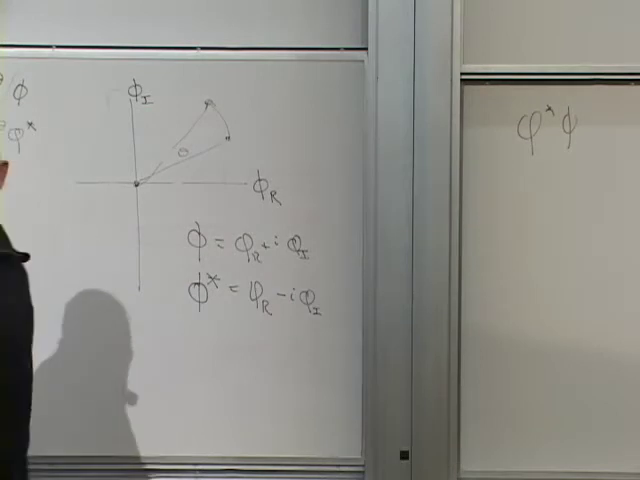
\includegraphics[width=0.80\textwidth]{lecture_07_figure_02.png}
\caption{Das komplexe Feld in der inneren \((\phi_R,\phi_I)\)-Ebene. An der Tafel werden die Zerlegung von \(\phi\)und \(\phi^*\)sowie der invariante Radius \(\phi^*\phi\)festgehalten.}
\lectureframe{00:33:33}
\end{figure}

Wir verwenden die Lagrange-Dichte
\begin{equation}
  \mathcal L
  =\partial_\mu\phi^*\,\partial^\mu\phi
   -V(\phi^*\phi).
  \label{eq:l07-complex-lagrangian}
\end{equation}
Bei einem komplexen Feld entfällt der übliche Faktor \(1/2\), denn dieses eine Produkt enthält bereits die kinetischen Terme beider reeller Komponenten. Die Transformation
\begin{equation}
  \phi'(x)=e^{i\theta}\phi(x),
  \qquad
  \phi^{*\prime}(x)=e^{-i\theta}\phi^*(x)
  \label{eq:l07-global-u1}
\end{equation}
dreht jeden Feldwert um denselben Winkel. Hier ist \(\theta\)räumlich und zeitlich konstant. Der Strich kennzeichnet das transformierte Feld; er steht nicht für eine Ableitung.

Da \(\theta\)konstant ist, gilt
\begin{equation}
  \partial_\mu\phi'=e^{i\theta}\partial_\mu\phi,
  \qquad
  \partial_\mu\phi^{*\prime}
  =e^{-i\theta}\partial_\mu\phi^*.
\end{equation}
Die Phasen heben sich im kinetischen Term auf, und
\(\phi^{*\prime}\phi'=\phi^*\phi\). Jedes Potential, das nur von \(\phi^*\phi\)abhängt, besitzt daher dieselbe Symmetrie. Ein Term, der allein von \(\phi_R\)abhängt, würde eine Richtung in der inneren Ebene auszeichnen und die Symmetrie explizit brechen.

\subsection{Ein punktförmiges Minimum und ein Kreis von Minima}

Es gibt zwei qualitativ verschiedene symmetrische Potentiale. Das erste hat sein einziges Minimum im Ursprung, zum Beispiel
\begin{equation}
  V_{\rm unbroken}=m^2\phi^*\phi,
  \qquad m^2>0.
\end{equation}
Sein Graph ist ein rotationssymmetrisches Paraboloid. Das Vakuum \(\phi=0\)bleibt unter jeder Drehung unverändert, die Symmetrie ist also ungebrochen.

Wählen wir nun
\begin{equation}
  V_{\rm broken}
  =-a\,\phi^*\phi+b(\phi^*\phi)^2,
  \qquad a,b>0.
  \label{eq:l07-mexican-hat}
\end{equation}
Der negative quadratische Term treibt das Feld vom Ursprung weg, während der positive quartische Term verhindert, dass es ins Unendliche läuft. Mit \(r^2=\phi^*\phi\)ergibt die Minimierung
\begin{equation}
  \frac{dV}{d(r^2)}=-a+2br^2=0,
  \qquad
  r^2=f^2=\frac{a}{2b}.
  \label{eq:l07-vacuum-radius}
\end{equation}
Die Minima bilden daher einen Kreis. Das Potential ist vollkommen rotationssymmetrisch, und doch muss ein homogener Grundzustand einen Punkt auf diesem Kreis auswählen.

\begin{figure}[htbp]
\centering
\includegraphics[width=0.72\textwidth]{lecture_07_figure_06.png}
\caption{Das Potential mit gebrochener Symmetrie als Rotationsfläche dargestellt. Der Ursprung ist instabil, und die entarteten Minima bilden die kreisförmige Rinne.}
\lectureframe{00:37:25}
\end{figure}

Man stelle sich das Feld an jedem Punkt des gewöhnlichen Raums als kleinen Pfeil in dieser inneren Ebene vor. Das Potential verlangt, dass jeder Pfeil die Länge \(f\)hat. Die Gradientenenergie verlangt, dass benachbarte Pfeile nahezu in dieselbe Richtung zeigen. Der Grundzustand hat folglich überall denselben Winkel, obwohl das Gesetz keinen Winkel bevorzugt. Das ist spontane Brechung einer kontinuierlichen Symmetrie.

\section{Von der Domänenwand zur glatten Verdrehung}

Wiederholen wir das Randbedingungsexperiment. Am linken Rand fixieren wir das Feld bei einem Vakuumpunkt \(A\); am rechten Rand fixieren wir es bei einem anderen Vakuumpunkt \(B\). Ein lokalisierter Sprung würde den Gradienten groß machen. Anders als im diskreten Fall kann das Feld jedoch am tiefsten Punkt des Potentials bleiben und sich dabei kontinuierlich um den Kreis bewegen.

Bei niedriger Energie schreiben wir das Feld als \(\phi=f e^{i\alpha(x)}\). In einer Raumdimension lautet die relevante Energie
\begin{equation}
  E[\alpha]
  =f^2\int_0^L dx\,\left(\frac{d\alpha}{dx}\right)^2.
  \label{eq:l07-angle-functional}
\end{equation}
Bei festgehaltenen Endwinkeln ergibt die Variation
\begin{equation}
  \frac{d^2\alpha}{dx^2}=0,
  \qquad
  \alpha(x)=\alpha_A+
    \frac{\alpha_B-\alpha_A}{L}\,x.
  \label{eq:l07-linear-twist}
\end{equation}
Die bevorzugte Konfiguration verteilt die Verdrehung gleichmäßig über die Probe. Ihre Energie skaliert wie
\begin{equation}
  E_{\rm twist}
  =f^2\frac{(\alpha_B-\alpha_A)^2}{L},
  \label{eq:l07-twist-energy}
\end{equation}
und lässt sich daher durch Vergrößern von \(L\)beliebig klein machen.

\begin{figure}[htbp]
\centering
\begin{adjustbox}{max width=\linewidth}
\begin{tikzpicture}[x=0.95cm,y=0.95cm]
  \begin{scope}
    \draw[->] (0,0) -- (6.2,0) node[right] {$x$};
    \draw[->] (0,0) -- (0,3.5) node[above] {$\alpha(x)$};
    \draw[very thick,blue!70!black] (0.45,0.65) -- (5.7,2.85);
    \fill (0.45,0.65) circle (1.8pt) node[left] {$\alpha_A$};
    \fill (5.7,2.85) circle (1.8pt) node[right] {$\alpha_B$};
    \node at (3.1,-0.65) {physical space};
  \end{scope}
  \begin{scope}[xshift=9.2cm,yshift=1.65cm]
    \draw[thick] (0,0) circle (1.8);
    \fill (1.55,-0.92) circle (1.8pt) node[below right] {$A$};
    \fill (-0.45,1.74) circle (1.8pt) node[above] {$B$};
    \draw[very thick,blue!70!black,-{Latex[length=2.5mm]}]
      (1.55,-0.92) arc[start angle=-31,end angle=104,radius=1.8];
    \node at (0,-2.35) {vacuum circle};
  \end{scope}
\end{tikzpicture}
\end{adjustbox}
\caption{Dieselbe Konfiguration niedriger Energie in zwei Darstellungen. Der Winkel variiert linear über den physikalischen Raum, während das Feld dem kurzen Kreisbogen des Vakuumkreises im inneren Raum folgt.}
\end{figure}

\begin{classroomqa}
\audiencequestion{Es gibt zwei Wege um den Kreis. Welchen Weg nimmt das Feld, und kann es auf dem längeren Weg gefangen bleiben?
\lecturetimestamp{00:41:54}}
\lecturerresponse{Für allgemeine Endpunkte hat der kürzere Weg entlang des Winkels den kleineren Gradienten und damit die niedrigere Energie. Bei diametral gegenüberliegenden Endpunkten sind die beiden einfachsten Wege entartet. Eine Konfiguration, die dadurch vorbereitet wurde, dass ein Endpunkt langsam bewegt wurde, kann eine zusätzliche Windung beibehalten und hinter einer Energiebarriere gefangen bleiben; für ein vorgegebenes Paar gewöhnlicher Endpunkte ist jedoch der unverdrillte kürzeste Weg der Grundzustand.}
\end{classroomqa}

\begin{classroomqa}
\audiencequestion{Könnte der Weg den Grund der Rinne verlassen und quer durch ihr Inneres verlaufen, sodass er insgesamt kürzer wäre?
\lecturetimestamp{00:43:32}}
\lecturerresponse{Im Bereich niedriger Energien und langer Proben lohnt es sich nicht, das radiale Potential hinaufzusteigen. Den Radius auf seinem Vakuumwert zu halten und den Winkel linear variieren zu lassen, minimiert die effektive Energie, wie die obige Variationsrechnung zeigt. Für ein endliches System mit einem konkreten Potential kann man radiale und winkelabhängige Bewegung gemeinsam minimieren; die Schlussfolgerung über Goldstone-Bosonen betrifft jedoch den Grenzfall beliebig großer Wellenlängen, in dem die glatte Bewegung entlang der Rinne energetisch günstiger ist.}
\end{classroomqa}

\begin{classroomqa}
\audiencequestion{Was ändert sich, wenn die kreisförmige Rinne verkippt wird, sodass ein Winkel tiefer liegt?
\lecturetimestamp{00:44:33}}
\lecturerresponse{Dann ist die Symmetrie explizit gebrochen. Ein Punkt wird zum echten Grundzustand, die Bewegung entlang des Kreises erhält eine Rückstellkraft, und die Winkelanregung ist nicht mehr exakt masselos.}
\end{classroomqa}

\section{Masse als Energie einer Oszillation bei verschwindendem Impuls}

Die glatte Verdrehung zeigt ein Feld, dessen Energie ausschließlich aus Gradienten stammt. Um zu verstehen, warum das ein masseloses Teilchen bedeutet, vergleichen wir die relativistische Dispersionsrelation
\begin{equation}
  \omega^2=\bm{k}^2+m^2.
  \label{eq:l07-dispersion}
\end{equation}
Eine Welle \(e^{i(\bm{k}\cdot\bm{x}-\omega t)}\)trägt den Impuls \(\bm{k}\). Ist \(m=0\), geht ihre Energie bei unendlich großer Wellenlänge gegen null:
\(\omega=|\bm{k}|\to0\). Ist \(m\ne0\), oszilliert ein räumlich homogener Modus \(\bm{k}=0\)dennoch mit der Frequenz \(\omega=m\). Die Masse ist die Energie, die auch bei verschwindendem Impuls unvermeidlich bleibt.

Derselbe Unterschied zeigt sich in der Lagrange-Dichte. Ein Term
\begin{equation}
  -\frac12m^2\varphi^2
\end{equation}
erzeugt selbst bei einer homogenen Auslenkung eine Rückstellkraft. Ein Feld, das nur Ableitungsterme enthält, besitzt keine solche Rückstellkraft: Je größer seine Wellenlänge, desto näher kommt seine Gradientenenergie an null.

\subsection{Polarkoordinaten trennen die beiden Moden}

Wir schreiben das komplexe Feld mit gebrochener Symmetrie als
\begin{equation}
  \phi(x)=\rho(x)e^{i\alpha(x)}.
  \label{eq:l07-polar}
\end{equation}
Sowohl \(\rho\)als auch \(\alpha\)sind Felder. Durch Ableiten erhalten wir
\begin{align}
  \partial_\mu\phi
  &=e^{i\alpha}
    \left(\partial_\mu\rho+i\rho\,\partial_\mu\alpha\right),\\
  \partial_\mu\phi^*
  &=e^{-i\alpha}
    \left(\partial_\mu\rho-i\rho\,\partial_\mu\alpha\right).
\end{align}
Die gemischten Terme heben sich auf, sodass
\begin{equation}
  \partial_\mu\phi^*\,\partial^\mu\phi
  =(\partial_\mu\rho)(\partial^\mu\rho)
   +\rho^2(\partial_\mu\alpha)(\partial^\mu\alpha).
  \label{eq:l07-polar-kinetic}
\end{equation}
Da \(\phi^*\phi=\rho^2\)gilt,
\begin{equation}
  \mathcal L
  =(\partial\rho)^2+\rho^2(\partial\alpha)^2-V(\rho^2).
  \label{eq:l07-polar-lagrangian}
\end{equation}
Das Potential enthält \(\rho\), aber nicht \(\alpha\). Darin zeigt sich die Symmetrie in ihrer nützlichsten Form.

\begin{figure}[htbp]
\centering
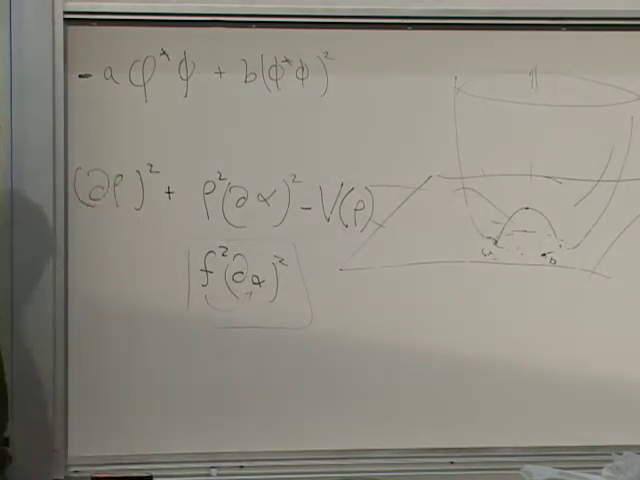
\includegraphics[width=0.88\textwidth]{lecture_07_figure_03.png}
\caption{Die Lagrange-Dichte in Polarkoordinaten, ihr eingerahmter Winkelterm bei niedriger Energie und das Potential mit gebrochener Symmetrie. Radiale Bewegung führt das Potential hinauf; Winkelbewegung folgt der Rinne.}
\lectureframe{00:56:40}
\end{figure}

Bei einer Anregung sehr niedriger Energie bleibt das Feld nahe bei \(\rho=f\). Dann gilt
\begin{equation}
  \mathcal L_{\rm angular}
  \simeq f^2(\partial_\mu\alpha)(\partial^\mu\alpha).
\end{equation}
Bis auf die Konvention für Faktoren von \(1/2\)definieren wir das kanonisch normierte Winkelfeld durch
\begin{equation}
  \beta=\sqrt{2}\,f\alpha,
  \qquad
  \mathcal L_{\rm angular}
  =\frac12(\partial_\mu\beta)(\partial^\mu\beta).
  \label{eq:l07-goldstone-field}
\end{equation}
Es gibt keinen Term \(\beta^2\). Die Quanten dieses Winkelfelds sind masselos. Sie sind die Goldstone-Bosonen.

Das Radialfeld verhält sich anders. Verschiebt man \(\rho\)überall gleichzeitig von \(f\)weg, rollt es zurück, überschwingt die Rinne und oszilliert um sie herum. Für \(\rho=f+h\)ergibt die Entwicklung von Gl.~\eqref{eq:l07-mexican-hat}
\begin{equation}
  V(f+h)=V(f)+\frac12m_h^2h^2+\cdots,
\end{equation}
sodass \(h\)massiv ist. Geometrisch ist die Winkelrichtung flach und die radiale Richtung gekrümmt.

\begin{classroomqa}
\audiencequestion{Wenn das Feld radial ausgelenkt wird, fällt es dann einfach zurück, und was geschieht danach?
\lecturetimestamp{00:57:10}}
\lecturerresponse{Ohne Winkelbewegung fällt es zum Minimum, überschwingt es und oszilliert radial. Eine homogene Oszillation hat verschwindenden räumlichen Impuls, aber eine von null verschiedene Frequenz; diese Frequenz ist die Masse der radialen Anregung. Eine homogene Winkelauslenkung landet dagegen in einem anderen Vakuum und erfährt keine Rückstellkraft.}
\end{classroomqa}

Das ist der Inhalt des Goldstone-Prinzips in diesem Beispiel: Die spontane Brechung einer kontinuierlichen globalen Symmetrie erzeugt für jede unabhängige flache Richtung der Vakuummannigfaltigkeit einen masselosen Modus.
\editorialnote{Die Aussage setzt die üblichen Bedingungen der relativistischen Feldtheorie voraus. In nichtrelativistischen Vielteilchensystemen kann die Zählung und Dispersion von Nambu---Goldstone-Moden subtiler sein, doch die Schlussfolgerung der Vorlesung für große Wellenlängen bleibt für dieses relativistische \(U(1)\)-Modell gültig.}

\section{Spinwellen, Saiten und Schall}

Der Satz ist abstrakt, doch der Mechanismus ist vertraut. In einem isotropen Ferromagneten können alle Spins gemeinsam gedreht werden, ohne die Energie zu ändern. Lässt man die Orientierung über die Probe hinweg sehr langsam variieren, erhält man eine Spinwelle. Ihre Energie geht mit der Wellenzahl gegen null; sie ist daher der Goldstone-Modus der gebrochenen Spin-Rotationssymmetrie.

Eine lange elastische Saite veranschaulicht den Gedanken ebenfalls. Wir vernachlässigen die Schwerkraft und befestigen die Enden so, dass die ganze Saite vertikal verschoben werden kann. Eine gleichförmige vertikale Verschiebung kostet keine Energie. Lässt man die Verschiebung entlang der Saite langsam variieren, entsteht eine Transversalwelle großer Wellenlänge. Die gleichförmige Symmetrieoperation wurde zu einer sanften ortsabhängigen Verformung verallgemeinert.

\begin{figure}[htbp]
\centering
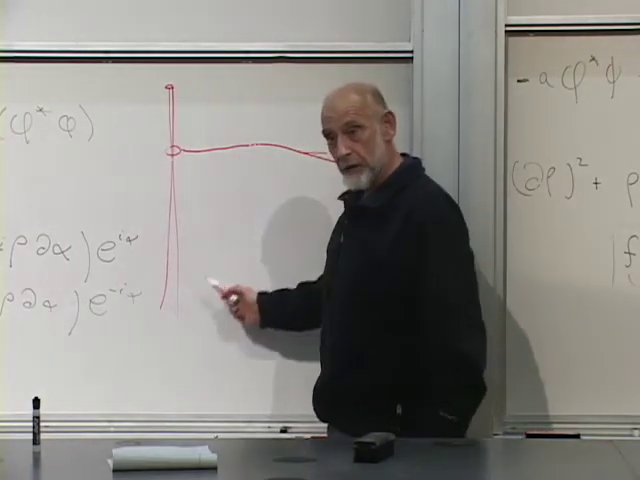
\includegraphics[width=0.68\textwidth]{lecture_07_figure_04.png}
\caption{Das langsam variierende Saitenprofil aus der Analogie zum Goldstone-Modus. Entscheidend ist die geringe Steigung einer Verformung mit großer Wellenlänge, nicht die vertikale Lage der Kurve.}
\lectureframe{01:04:19}
\end{figure}

\begin{classroomqa}
\audiencequestion{Kann die Saite Schwingungsenergie tragen, obwohl sie keinen Impuls hat?
\lecturetimestamp{01:04:41}}
\lecturerresponse{Man muss den vertikalen mechanischen Impuls vom Wellenimpuls entlang der Saite unterscheiden. Eine stehende Welle kann verschwindenden Gesamtimpuls haben, weil sie eine Überlagerung von Moden mit \(+k\)und \(-k\)ist, und dennoch Energie tragen. In der feldtheoretischen Analogie bezieht sich der Impuls auf die Wellenzahl entlang der Achse; die vertikale Auslenkung steht für die innere Feldkoordinate.}
\end{classroomqa}

Eine Slinky-Feder veranschaulicht den longitudinalen Fall. Verschiebt man die gesamte idealisierte unendliche Slinky-Feder entlang ihrer Achse, ändert sich nichts. Verschiebt man benachbarte Teile um geringfügig unterschiedliche Beträge, entsteht eine sanfte Kompressionswelle. In einem Festkörper oder einer Flüssigkeit entsteht langwelliger Schall auf ähnliche Weise durch kollektive Verschiebungen und Dichteänderungen. Spinwellen, transversale Saitenwellen und Schall sind nicht dieselbe mikroskopische Anregung, doch sie weisen dasselbe entscheidende Muster auf: Eine gleichförmige kontinuierliche Operation kostet keine Energie, und ihre langsam variierende Version wird zu einem weichen Modus.
\editorialnote{In einem Kristall werden akustische Phononen üblicherweise als Nambu---Goldstone-Moden der spontan gebrochenen kontinuierlichen Translationssymmetrie beschrieben. Saite und Slinky-Feder dienen in der Vorlesung als mechanische Analogien, die dieselbe Ableitungsstruktur der Energie veranschaulichen.}

Die Bezeichnung verdient einen kurzen Scherz aus der Vorlesung: Es sind \emph{Goldstone}-Bosonen, benannt nach Jeffrey Goldstone, und keine Eichbosonen. Die Vorlesung erwähnt, dass Goldstone ein Freund Susskinds war, und wendet sich dann dem tatsächlich anderen Thema der Eichinvarianz zu.

\section{Von globaler Phasensymmetrie zur Eichsymmetrie}

Die Phasensymmetrie \(U(1)\)ist im Kurs bereits als die mit der Ladungserhaltung verknüpfte Symmetrie aufgetreten. Felder geladener Teilchen sind komplex, und die Multiplikation eines solchen Feldes mit einer gemeinsamen Phase lässt die globale Theorie unverändert. Zur Veranschaulichung kann man von elektrischer Ladung sprechen, doch die Ladung könnte auch eine andere Quantenzahl \(U(1)\)darstellen. Das reale Photon ist masselos; das spätere Ziel ist ein photonartiges Feld wie das massive \(Z\).

Die neue Frage lautet, ob
\begin{equation}
  \phi'(x)=e^{i\theta(x)}\phi(x)
  \label{eq:l07-local-u1}
\end{equation}
eine Symmetrie sein kann, wenn \(\theta\)beliebig durch die Raumzeit variiert. Die Funktion \(\theta(x)\)ist ein Transformationsparameter und kein zusätzliches dynamisches Feld. Wir prüfen den Vorschlag, indem wir ableiten:
\begin{equation}
  \partial_\mu\phi'
  =e^{i\theta}
   \left[\partial_\mu\phi+i(\partial_\mu\theta)\phi\right].
  \label{eq:l07-local-derivative}
\end{equation}
Der zusätzliche Term fehlte bei konstantem \(\theta\). Für das konjugierte Feld gilt
\begin{equation}
  \partial_\mu\phi^{*\prime}
  =e^{-i\theta}
   \left[\partial_\mu\phi^*-i(\partial_\mu\theta)\phi^*\right].
\end{equation}
Ihr Produkt lautet
\begin{align}
  \partial_\mu\phi^{*\prime}\partial^\mu\phi'
  ={}&
  \partial_\mu\phi^*\partial^\mu\phi
  i\left(
      \phi\,\partial_\mu\phi^*
      -\phi^*\partial_\mu\phi
    \right)\partial^\mu\theta
  \nonumber\\
  &+\phi^*\phi\,
    \partial_\mu\theta\,\partial^\mu\theta.
  \label{eq:l07-local-failure}
\end{align}
Das Potential bleibt invariant, weil es nur von \(\phi^*\phi\)abhängt; der gewöhnliche kinetische Term ist es jedoch nicht. Eine globale Symmetrie wird nicht automatisch zu einer lokalen.

\begin{classroomqa}
\audiencequestion{Bedeutet dieses Versagen im Mexican-Hat-Bild, dass es Unebenheiten entlang der kreisförmigen Rinne gibt?
\lecturetimestamp{01:19:37}}
\lecturerresponse{Nein. Das Potential kann in Winkelrichtung vollkommen flach bleiben. Die zusätzlichen Kosten entstehen durch Gradienten, wenn sich die Phase von einem Raumzeitpunkt zum anderen unterscheidet. Es handelt sich nicht um eine Verformung der Rinne; vielmehr registriert der gewöhnliche Ableitungsterm die räumliche Variation.}
\end{classroomqa}

\subsection{Das kompensierende Vektorfeld}

Die Wechselwirkungen des Photons \(W\), des \(Z\)-Bosons und der Gluonen werden durch lokale Eichsymmetrien organisiert, nicht bloß durch starre Transformationen. Damit die lokale Phasenoperation eine Symmetrie ist, erweitern wir die Theorie um ein Vierervektorfeld \(A_\mu\). In der Elektrodynamik ist \(A_0\)das skalare Potential; die drei räumlichen Komponenten bilden das Vektorpotential. Aus ihren Ableitungen entstehen das elektrische und das magnetische Feld.

Wir wählen die in sich konsistente Konvention
\begin{equation}
  \phi'=e^{i\theta}\phi,
  \qquad
  A'_\mu=A_\mu-\partial_\mu\theta,
  \qquad
  D_\mu=\partial_\mu+iA_\mu.
  \label{eq:l07-gauge-convention}
\end{equation}
Beim Überprüfen der Aufhebung ändert sich an der Tafel ein Vorzeichen; Gl. \eqref{eq:l07-gauge-convention}legt alle drei Vorzeichen gemeinsam fest. Die Eichkopplung und die Ladung sind vorübergehend in \(A_\mu\)aufgenommen worden.
\editorialnote{Mit expliziter Ladung \(q\)und Kopplung \(g\)kann man schreiben:
\(D_\mu=\partial_\mu+igqA_\mu\)und
\(A'_\mu=A_\mu-(gq)^{-1}\partial_\mu\theta\). In der Vorlesung werden diese Konstanten weggelassen, damit die Aufhebung sichtbar bleibt.}

Für das konjugierte Feld gilt
\begin{equation}
  D_\mu\phi^*=\partial_\mu\phi^*-iA_\mu\phi^*.
\end{equation}
Nun ist
\begin{align}
  D'_\mu\phi'
  &=
  \left(\partial_\mu+iA'_\mu\right)e^{i\theta}\phi
  \nonumber\\
  &=
  e^{i\theta}
  \left[
    \partial_\mu\phi+i(\partial_\mu\theta)\phi
    +i(A_\mu-\partial_\mu\theta)\phi
  \right]
  \nonumber\\
  &=e^{i\theta}D_\mu\phi.
  \label{eq:l07-covariant-transform}
\end{align}
Die unerwünschte Ableitung von \(\theta\)wird durch die Transformation von \(A_\mu\)aufgehoben. Ebenso gilt
\begin{equation}
  D'_\mu\phi^{*\prime}=e^{-i\theta}D_\mu\phi^*.
\end{equation}
Ihr Produkt ist invariant. Das Adjektiv \emph{kovariant}bedeutet, dass sich die Ableitung auf dieselbe einfache Weise transformiert wie das Feld selbst.

\section{Dynamik des Eichfelds}

Würden wir \(A_\mu\)nur einführen, um eine Ableitung zu korrigieren, hätte das Feld keine eigene Dynamik. Der eichinvariante Feldstärketensor ist
\begin{equation}
  F_{\mu\nu}
  =\partial_\mu A_\nu-\partial_\nu A_\mu.
  \label{eq:l07-field-strength}
\end{equation}
Er ist antisymmetrisch, also gilt \(F_{\mu\mu}=0\). Seine Zeit--Raum-Komponenten enthalten das elektrische Feld, seine Raum--Raum-Komponenten das magnetische Feld. In der vertrauten Vektorschreibweise ist die elektromagnetische Energiedichte proportional zu \(\bm E^2+\bm B^2\), während die Lagrange-Dichte in Lorentz-Signatur proportional zu \(\bm E^2-\bm B^2\)ist; die Vorzeichen hängen von der Metrikkonvention ab.

\begin{classroomqa}
\audiencequestion{Wie lauten Energie und Lagrange-Dichte des elektromagnetischen Feldes?
\lecturetimestamp{01:33:20}}
\lecturerresponse{Die Energie wird aus \(E^2+B^2\)gebildet; in der Lagrange-Dichte steht \(E^2-B^2\). Kovariant schreibt man Letztere als ein übliches Vielfaches von \(F_{\mu\nu}F^{\mu\nu}\). Der antisymmetrische Tensor ist die vierdimensionale Rotation des Vektorpotentials.}
\end{classroomqa}

Die Feldstärke ist selbst eichinvariant:
\begin{align}
  F'_{\mu\nu}
  &=
  \partial_\mu(A_\nu-\partial_\nu\theta)
  -\partial_\nu(A_\mu-\partial_\mu\theta)
  \nonumber\\
  &=
  F_{\mu\nu}
  -\partial_\mu\partial_\nu\theta
  +\partial_\nu\partial_\mu\theta
  =F_{\mu\nu}.
  \label{eq:l07-field-strength-invariant}
\end{align}
Die letzte Gleichheit folgt daraus, dass gewöhnliche gemischte partielle Ableitungen vertauschen. Eine übliche eichinvariante Lagrange-Dichte lautet daher
\begin{equation}
  \boxed{
  \mathcal L
  =(D_\mu\phi)^*D^\mu\phi
  -V(\phi^*\phi)
  -\frac14F_{\mu\nu}F^{\mu\nu}}
  \label{eq:l07-scalar-qed}
\end{equation}
bis auf die Vorzeichen- und Normierungskonventionen der Metrik.

\begin{figure}[htbp]
\centering
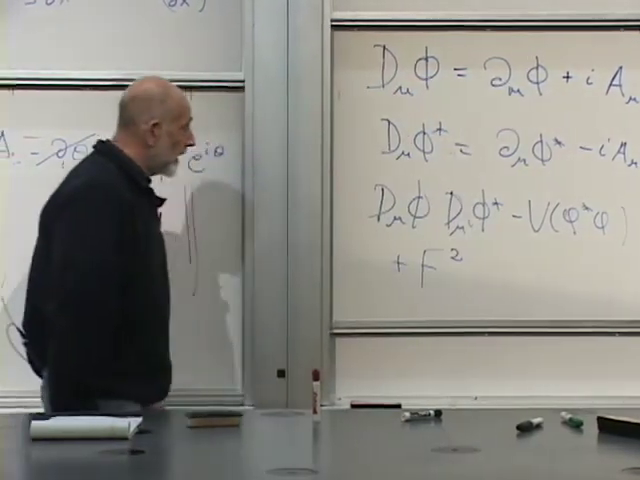
\includegraphics[width=0.84\textwidth]{lecture_07_figure_05.png}
\caption{Die kovarianten Ableitungen und die an der Tafel zusammengestellte eichinvariante Lagrange-Dichte. Numerische Faktoren werden dort weggelassen, damit die Transformationsstruktur sichtbar bleibt.}
\lectureframe{01:38:45}
\end{figure}

Diese Konstruktion macht aus einer globalen \(U(1)\)-Symmetrie eine lokale; dafür müssen wir jedoch---oder, physikalisch gesehen, als Geschenk---ein neues Vektorfeld einführen. Im abelschen Beispiel ist dieses Feld das elektromagnetische Potential.

\begin{classroomqa}
\audiencequestion{In der Lagrange-Dichte, von der wir ausgegangen sind, standen gewöhnliche Ableitungen. Warum dürfen wir sie durch kovariante Ableitungen ersetzen und das Ergebnis als die eigentliche Theorie bezeichnen?
\lecturetimestamp{01:42:55}}
\lecturerresponse{Wir konstruieren eine andere, erweiterte Theorie: geladene Materie zusammen mit einem Eichfeld. Die lokale Eichinvarianz legt ihre Kopplung fest. Die resultierende Quantentheorie ist eine in sich schlüssige mathematische Struktur und stimmt damit überein, wie die Natur das Photon und die schwachen Eichfelder organisiert. Eine relativistische Vektorfeldtheorie einfach auf inkonsistente Weise zu koppeln, kann unphysikalische Polarisationen und Verletzungen der Wahrscheinlichkeitserhaltung zur Folge haben; das Eichprinzip ist also keine kosmetische Umschreibung der alten Theorie eines freien Skalarfelds.}
\end{classroomqa}

\begin{classroomqa}
\audiencequestion{Ist das Hinzufügen des neuen Feldes also die entscheidende Begründung für die Modifikation?\lecturetimestamp{01:44:57}}
\lecturerresponse{Ja. Ohne \(A_\mu\) enthält die Ableitung eines lokal gedrehten Feldes einen nicht kompensierten Term \(\partial_\mu\theta\). Mit \(A_\mu\) und seinem Transformationsgesetz funktioniert die Aufhebung. In der Sprache der Geometrie ist \(A_\mu\) eine Verbindung auf einem Bündel; diese weiterführende Mathematik ist real und nützlich, doch die obige Algebra enthält bereits alles, was wir hier benötigen.}
\end{classroomqa}

\section{Warum eine nackte Eichbosonenmasse verboten ist}

Für ein gewöhnliches bosonisches Feld wird eine Masse durch einen quadratischen Term dargestellt. Es liegt nahe, folgenden Term hinzuzufügen:
\begin{equation}
  \Delta\mathcal L_{\rm Proca}
  =\frac12m^2A_\mu A^\mu.
  \label{eq:l07-proca}
\end{equation}
Unter \(A_\mu\mapsto A_\mu-\partial_\mu\theta\) gilt jedoch
\begin{equation}
  A'_\mu A^{\mu\prime}
  =
  A_\mu A^\mu
  -2A^\mu\partial_\mu\theta
  +\partial_\mu\theta\,\partial^\mu\theta,
\end{equation}
sodass Gleichung ~\eqref{eq:l07-proca} nicht eichinvariant ist. Wir können dieser Eichtheorie nicht von Hand eine Masse hinzufügen und dabei ihre lokale Symmetrie bewahren.

\begin{figure}[htbp]
\centering
\includegraphics[width=0.72\textwidth]{lecture_07_figure_07.png}
\caption{Die vorgeschlagene nackte Vektormasse
\(\tfrac12m^2A_\mu A^\mu\). Ihr Versagen unter
\(A_\mu\mapsto A_\mu-\partial_\mu\theta\) ist das Hindernis, das den Higgs-Mechanismus vorbereitet.}
\lectureframe{01:39:48}
\end{figure}

Hier zeigt sich der scheinbare Widerspruch. Die Eichinvarianz erklärt das masselose Photon und schützt die Theorie vor unphysikalischen Freiheitsgraden, doch \(W\) und \(Z\) sind massiv. Der Ausweg kann keine explizite Vektormasse sein. Er muss aus den bereits in einer eichinvarianten Lagrange-Dichte vorhandenen Feldern hervorgehen.

\begin{classroomqa}
\audiencequestion{Entsteht das Goldstone-Boson durch die Einführung der Eichinvarianz selbst?\lecturetimestamp{01:45:51}}
\lecturerresponse{Nein. Das Goldstone-Boson entstand, als eine kontinuierliche \emph{globale} Symmetrie spontan gebrochen wurde, noch bevor das Vektorpotential eingeführt wurde. Sobald die Symmetrie lokal ist, kann eine ortsabhängige Phase durch \(A_\mu\) kompensiert werden. In der gebrochenen Eichtheorie ist der Winkelmodus kein unabhängiges masseloses Teilchen mehr; er liefert die zusätzliche Polarisation des nun massiven Vektorfeldes. In der nächsten Vorlesung wird diese Aussage hergeleitet und nicht bloß verkündet.}
\end{classroomqa}

\begin{classroomqa}
\audiencequestion{Erklärt irgendetwas davon, warum Flüsse mäandrieren?
\lecturetimestamp{01:47:03}}
\lecturerresponse{Ein direkter Zusammenhang ist hier nicht bekannt. Strömungswirbel und sogar die Formen von Organismen lassen sich durchaus mit Methoden der Symmetrie beschreiben, und es sollte uns nie überraschen, feldtheoretischen Ideen an unerwarteten Stellen zu begegnen; diese Vorlesung behauptet jedoch keine Eichtheorie der Flussmäander.}
\end{classroomqa}

\section{Wo die Vorlesung endet}

Nun haben wir die beiden zu Beginn angekündigten Zutaten. Eine kontinuierliche globale Symmetrie mit einem Kreis von Vakuumzuständen besitzt eine flache Winkelrichtung, und ihre langsame Variation ist ein masseloses Goldstone-Feld. Eine lokale Symmetrie erfordert eine Eichverbindung und kovariante Ableitungen; außerdem verbietet sie die direkte Vektormasse in Gleichung ~\eqref{eq:l07-proca}.

Der nächste Schritt besteht darin, das gebrochene Potential aus Gleichung ~\eqref{eq:l07-mexican-hat} innerhalb der eichinvarianten Theorie aus Gleichung ~\eqref{eq:l07-scalar-qed} zu verwenden. Dann geschehen zwei Dinge zugleich: Das separate Goldstone-Teilchen verschwindet aus dem physikalischen Spektrum, und das Vektorfeld erhält eine Masse. In der üblichen didaktischen Ausdrucksweise wird die Eichsymmetrie spontan gebrochen; genauer gesagt bleibt die Eichredundanz bestehen, während die Theorie in eine Higgs-Phase mit einer massiven Vektoranregung eintritt.
\editorialnote{Eine lokale Eichsymmetrie ist eine Redundanz der Beschreibung und keine gewöhnliche physikalische Symmetrie, die zwischen verschiedenen beobachtbaren Zuständen wirkt. Die Vorlesung verwendet die übliche Kurzform der spontanen Eichsymmetriebrechung. Die eichinvariante physikalische Aussage ist die Neuordnung der Freiheitsgrade in der Higgs-Phase.}

Das ist das Higgs-Phänomen. Wir haben es noch nicht durchgeführt. Diese Vorlesung hat die notwendige, anspruchsvollere Arbeit geleistet: Sie hat das Problem so präzise gefasst, dass die Lösung, wenn sie kommt, unausweichlich sein wird.
\chapter{Der Higgs-Mechanismus: Wie ein Eichboson Masse erhält}

Wir verbinden nun die beiden Ideen aus der vorherigen Vorlesung. Ein komplexes Skalarfeld mit gebrochener globaler \(U(1)\)-Symmetrie besitzt eine massive radiale Schwingung und eine masselose Winkelschwingung. Eine lokal invariante \(U(1)\)-Theorie enthält ein masseloses Eichfeld. Ist das Skalarfeld geladen und sein Gleichgewichtsbetrag ungleich null, lassen sich diese Aussagen nicht einfach zusammenfügen. Der Winkelmodus und das Eichfeld verbinden sich: Das Eichfeld wird massiv, das scheinbare Goldstone-Boson ist kein unabhängiges Teilchen mehr, und der radiale Higgs-Modus bleibt erhalten.

Das Photon dient uns als Modell-Eichboson, nicht aber als physikalische Schlussfolgerung. Die elektromagnetische \(U(1)\)-Symmetrie ist im Vakuum nicht gebrochen, daher ist das reale Photon masselos. Derselbe Mechanismus wirkt in der elektroschwachen Theorie auf das \(W^\pm\) und das \(Z\); dort sind die Eichgruppe und das Skalarmultiplett komplizierter. Das abelsche Modell macht den Mechanismus sichtbar, ohne ihn hinter Gruppentheorie zu verbergen.

\begin{classroomqa}
\audiencequestion{Bedeutete die vorherige Diskussion, dass der Higgs-Mechanismus dem realen Photon Masse verleiht?\lecturetimestamp{00:00:23}}
\lecturerresponse{Nein. Wir fragen, was geschehen würde, \emph{wenn} die mit dem Photon verbundene \(U(1)\)-Symmetrie gebrochen wäre. Dieses hypothetische Photon würde massiv. Das reale elektromagnetische Vakuum befindet sich nicht in dieser Phase; in der Teilchenphysik geht es stattdessen um die Masse des \(W\) und des \(Z\).}
\end{classroomqa}

Die mit der Erhaltung der elektrischen Ladung verbundene Symmetrie ist die Phasendrehung
\begin{equation}
  \phi(x)\longmapsto e^{i\theta}\phi(x),
\end{equation}
eine interne Drehung, die als \(U(1)\) bezeichnet wird. Ein Supraleiter bietet ein reales Analogon der gebrochenen Phase. In seinem Inneren hat das elektromagnetische Feld eine endliche Eindringtiefe und verhält sich in wichtigen Hinsichten wie ein massives Feld. Außerhalb tritt wieder das gewöhnliche masselose Photon auf.

\section{Was Masse für ein Feld bedeutet}

\subsection{Dispersion und die Lücke bei verschwindendem Impuls}

Bevor wir das Higgs-Feld einführen, sollten wir genau festlegen, was wir unter Masse verstehen. Für eine Welle gilt
\begin{equation}
  E=\hbar\omega,
  \qquad
  p=\hbar k,
  \label{eq:l08-quantum-wave}
\end{equation}
Ein \((E,p)\)-Diagramm und ein \((\omega,k)\)-Diagramm enthalten also bis auf Faktoren von \(\hbar\) dieselbe Information. Im leeren Raum erfüllt eine masselose relativistische Anregung
\begin{equation}
  E=c|p|,
  \qquad
  \omega=c|k|.
  \label{eq:l08-massless-dispersion}
\end{equation}
Die beiden Vorzeichen von \(k\) kennzeichnen entgegengesetzte Ausbreitungsrichtungen. Entscheidend ist, dass \(\omega\) mit \(k\) gegen null geht.

Für ein massives relativistisches Teilchen gilt
\begin{equation}
  E^2=c^2p^2+m^2c^4.
  \label{eq:l08-massive-dispersion}
\end{equation}
In Einheiten mit \(c=\hbar=1\) gilt
\begin{equation}
  \omega^2=k^2+m^2.
\end{equation}
Bei \(k=0\) beträgt die Energie \(E=mc^2\), oder in natürlichen Einheiten einfach \(m\). Masse ist somit die von null verschiedene Energielücke des Modus mit verschwindendem Impuls.

\begin{figure}[htbp]
\centering
\begin{adjustbox}{max width=\linewidth}
\begin{tikzpicture}[x=1.05cm,y=1.05cm]
  \begin{scope}
    \draw[->] (-0.2,0) -- (4.2,0) node[right] {\(k\)};
    \draw[->] (0,-0.2) -- (0,3.1) node[above] {\(\omega\)};
    \draw[very thick,blue!65!black] (0,0) -- (3.8,2.75);
    \draw[very thick,orange!70!black] (0,0) -- (3.8,1.75);
    \node[blue!65!black,rotate=36] at (2.65,2.15)
      {\(\omega=c_{\rm vac}k\)};
    \node[orange!70!black,rotate=24] at (2.65,1.05)
      {ordinary medium};
    \node[below] at (2,-0.45) {gapless};
  \end{scope}
  \begin{scope}[xshift=6.2cm]
    \draw[->] (-0.2,0) -- (4.2,0) node[right] {\(k\)};
    \draw[->] (0,-0.2) -- (0,3.1) node[above] {\(\omega\)};
    \draw[very thick,domain=0:3.8,samples=120,smooth,teal!70!black]
      plot (\x,{sqrt(0.9+0.45*\x*\x)});
    \draw[dashed] (0,0.95) -- (1.0,0.95);
    \node[left] at (0,0.95) {\(m\)};
    \node[teal!70!black] at (2.55,2.15)
      {\(\omega^2=k^2+m^2\)};
    \node[below] at (2,-0.45) {gapped};
  \end{scope}
\end{tikzpicture}
\end{adjustbox}
\caption{Eine Änderung der Ausbreitungsgeschwindigkeit ändert die Steigung einer lückenlosen Dispersionsrelation. Eine Masse der Anregung öffnet bei \(k=0\) eine endliche Lücke.}
\label{fig:l08-dispersion}
\end{figure}

Ein gewöhnliches transparentes Material kann die Phasengeschwindigkeit einer Welle herabsetzen, ohne diese relativistische Masselücke zu erzeugen. An einer Grenzfläche bleibt die Frequenz der einfallenden Welle fest, während sich die Wellenzahl an die Dispersionsrelation des Mediums anpasst. Die Steigung zu ändern ist nicht dasselbe, wie den Achsenabschnitt anzuheben.
\editorialnote{Ein Material kann mehrere elektromagnetische Zweige besitzen, und in einem Plasma oder einem resonanten Medium kann eine endliche Plasmafrequenzlücke auftreten. Der Vergleich in dieser Vorlesung betrifft ausdrücklich einen gewöhnlichen Brechungszweig und die Antwort eines Supraleiters. Allgemeiner bedeutet Lückenlosigkeit, dass \(\omega(k)\to0\) für \(k\to0\) gilt; exakte Linearität ist nicht in jedem nichtrelativistischen Medium erforderlich.}

\begin{classroomqa}
\audiencequestion{Erhält ein Photon immer dann Masse, wenn es sich durch Materie bewegt, zum Beispiel durch ein Prisma?\lecturetimestamp{00:03:02}}
\lecturerresponse{Nein. Die Brechung kann die Beziehung zwischen Frequenz und Wellenzahl und damit die Ausbreitungsgeschwindigkeit ändern, während der Zweig bei \(\omega=0\) weiterhin durch \(k=0\) verläuft. In einer supraleitenden Phase erhält die elektromagnetische Antwort dagegen eine endliche inverse Eindringlänge, das Analogon einer Masse.}
\end{classroomqa}

\begin{classroomqa}
\audiencequestion{Ändert sich die Wellenzahl, wenn Licht mit fester Frequenz in Glas eintritt?\lecturetimestamp{00:09:20}}
\lecturerresponse{Ja. Die Zeittranslationsinvarianz an einer stationären Grenzfläche hält die Frequenz konstant. Da die Dispersionskurve im Glas eine andere Steigung hat, entspricht dasselbe \(\omega\) einem anderen \(k\) und damit einer anderen Wellenlänge.}
\end{classroomqa}

Die Steigung
\begin{equation}
  v_g=\frac{d\omega}{dk}
\end{equation}
ist die Gruppengeschwindigkeit eines Wellenpakets. Ändert sich diese Steigung mit \(k\), bewegen sich verschiedene Fourier-Komponenten mit unterschiedlichen Geschwindigkeiten, und das Paket dispersiert. Deshalb heißt die Beziehung \(\omega(k)\) \emph{Dispersionsrelation}.

\begin{classroomqa}
\audiencequestion{Wie heißt die Kurve, und was bedeutet ihre Steigung?\lecturetimestamp{00:11:02}}
\lecturerresponse{Die Kurve ist die Dispersionsrelation. Ihre Ableitung \(d\omega/dk\) ist die Gruppengeschwindigkeit. Bei konstanter Steigung haben alle Wellenlängen dieselbe Geschwindigkeit; bei veränderlicher Steigung breitet sich ein Wellenpaket aus. Für unseren Zweck ist entscheidend, ob die Kurve den Ursprung erreicht oder eine Lücke aufweist.}
\end{classroomqa}

\subsection{Eine homogene Schwingung entspricht einem Teilchen in Ruhe}

Der Modus \(k=0\) hat eine unendliche Wellenlänge: Das Feld ist überall um denselben Betrag ausgelenkt. Gibt man eine homogene Auslenkung frei, so schwingt das Feld mit einer von null verschiedenen Frequenz, falls die zugehörige Quante eine von null verschiedene Ruheenergie besitzt und damit massiv ist. Fehlt in dieser Richtung eine rücktreibende Kraft, verschwindet die Frequenz und der Modus ist masselos.

Diese Aussage ist klassisch. Sie setzt nicht voraus, dass räumlich getrennte Teilchen sich in einer quantenmechanischen Superposition befinden. Eine homogene klassische Feldkonfiguration ist schlicht ein Feldwert, der im gesamten Raum denselben Wert hat.

\begin{classroomqa}
\audiencequestion{Wenn ein ganzes Feld gemeinsam verschoben wird, ist das dasselbe wie Quantenverschränkung?\lecturetimestamp{00:10:04}}
\lecturerresponse{Nein. Ein homogenes klassisches Feld ist eine einzige klassische Konfiguration. Verschränkung korreliert verschiedene Quantenalternativen, etwa die Spinkonfigurationen oben--unten und unten--oben. An vielen Orten denselben Feldwert einzustellen, ist für sich genommen keine Verschränkung und bedeutet auch keine augenblickliche kausale Reaktion.}
\end{classroomqa}

Für ein kanonisch normiertes reelles Feld gilt
\begin{equation}
  \mathcal L
  =\frac12\partial_\mu\varphi\,\partial^\mu\varphi-V(\varphi),
\end{equation}
Wir entwickeln um ein Gleichgewicht \(\varphi_0\):
\begin{equation}
  V(\varphi_0+\eta)
  =V(\varphi_0)
   +\frac12V''(\varphi_0)\eta^2+\cdots.
\end{equation}
Am Minimum verschwindet der lineare Term, und die Feldgleichung ergibt
\begin{equation}
  \omega^2=\bm{k}^2+m^2,
  \qquad
  m^2=V''(\varphi_0).
  \label{eq:l08-curvature-mass}
\end{equation}
Die Masse entspricht somit der Krümmung des Potentials in Bewegungsrichtung. Eine flache Richtung hat keine Krümmung und ergibt einen masselosen Modus.

\section{Das gebrochene komplexe Skalarfeld}

\subsection{Radiale und tangentiale Bewegung}

Wir schreiben ein komplexes Skalarfeld in kartesischen und Polarkoordinaten:
\begin{equation}
  \phi=\phi_R+i\phi_I=\rho e^{i\alpha},
  \qquad
  \phi^*=\phi_R-i\phi_I=\rho e^{-i\alpha}.
  \label{eq:l08-polar-field}
\end{equation}
Die komplexe Ebene ist ein \emph{interner} Feldraum. An jedem physikalischen Raumzeitpunkt \(x\) legt das Paar
\((\phi_R(x),\phi_I(x))\)einen Punkt in dieser internen Ebene fest.
Keine der beiden internen Achsen ist eine Richtung im Labor.

\begin{figure}[htbp]
\centering
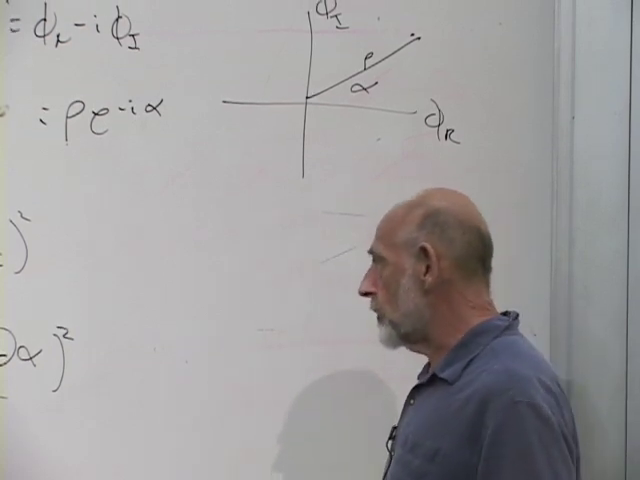
\includegraphics[width=0.72\textwidth]{lecture_08_figure_02.png}
\caption{Das komplexe Skalarfeld in seiner internen \((\phi_R,\phi_I)\)-Ebene. Der Radius ist \(\rho\), und \(\alpha\) bezeichnet die interne Phase.}
\lectureframe{00:24:41}
\label{fig:l08-internal-plane}
\end{figure}

Der kinetische Term des Skalarfelds wird zu
\begin{align}
  \partial_\mu\phi^*\,\partial^\mu\phi
  &=
  \partial_\mu\phi_R\,\partial^\mu\phi_R
  +\partial_\mu\phi_I\,\partial^\mu\phi_I
  \notag\\
  &=
  \partial_\mu\rho\,\partial^\mu\rho
  +\rho^2\partial_\mu\alpha\,\partial^\mu\alpha.
  \label{eq:l08-polar-kinetic}
\end{align}
Ein globales \(U(1)\)-invariantes Potential hängt von \(\phi^*\phi=\rho^2\) ab, nicht von \(\alpha\). Zum Beispiel:
\begin{equation}
  V(\phi)
  =\lambda\left(\phi^*\phi-\frac{f^2}{2}\right)^2,
  \qquad \lambda>0.
  \label{eq:l08-mexican-hat}
\end{equation}
Die Minima bilden einen Kreis. Das Gesetz ist unter einer gemeinsamen Phasendrehung invariant, doch die Wahl einer Gleichgewichtsphase zeichnet einen Punkt auf dem Kreis aus.

\begin{figure}[htbp]
\centering
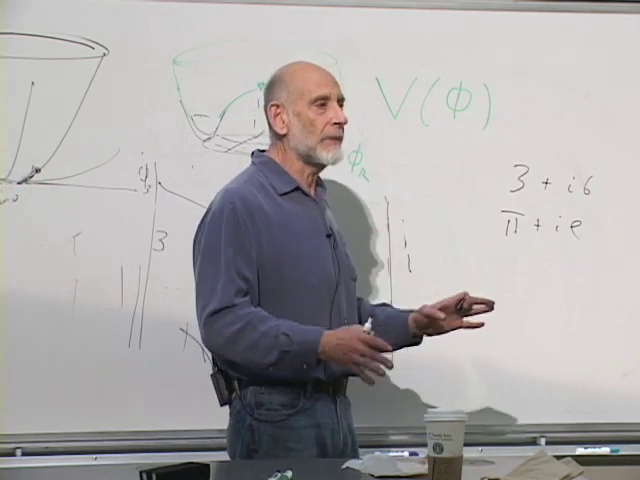
\includegraphics[width=0.78\textwidth]{lecture_08_figure_03.png}
\caption{Skizzen des radialen Potentials an der Tafel. Das Potential ist gegenüber Drehungen des internen Feldwerts symmetrisch, obwohl das Feld selbst nicht im Ursprung liegen muss.}
\lectureframe{00:34:22}
\label{fig:l08-radial-potential-board}
\end{figure}

\begin{figure}[htbp]
\centering
\begin{tikzpicture}[x=0.94cm,y=0.94cm]
  \draw[->] (-4.2,0) -- (4.4,0) node[right] {\(\phi_R\)};
  \draw[->] (0,-3.7) -- (0,3.9) node[above] {\(\phi_I\)};
  \draw[very thick,blue!65!black] (0,0) circle (2.45);
  \draw[->,very thick,orange!75!black] (0,0) -- (2.2,1.08);
  \draw[->,very thick,teal!70!black]
    (2.2,1.08) arc[start angle=26,end angle=67,radius=2.45];
  \node[orange!75!black,below right] at (1.15,0.52)
    {radial \(h\): massive};
  \node[teal!70!black,above right] at (1.78,1.76)
    {angular \(\pi\): massless};
  \fill (2.2,1.08) circle (2pt);
  \node[below] at (0,-2.65) {degenerate vacuum circle};
\end{tikzpicture}
\caption{Die global gebrochene Theorie besitzt eine Krümmung senkrecht zum Vakuumkreis, aber keine Krümmung entlang des Kreises. Der radiale Higgs-Modus ist massiv, der winkelabhängige Goldstone-Modus masselos.}
\label{fig:l08-radial-angular}
\end{figure}

Wir setzen
\begin{equation}
  \phi(x)=\frac{f+h(x)}{\sqrt2}
           e^{i\pi(x)/f}.
  \label{eq:l08-canonical-polar}
\end{equation}
In der Nähe des ausgewählten Vakuums beschreibt \(h\) die radiale Auslenkung und \(\pi\) die tangentiale Auslenkung, jeweils mit kanonischer Normierung. Einsetzen in Gl.~\eqref{eq:l08-polar-kinetic} ergibt
\begin{equation}
  \partial_\mu\phi^*\,\partial^\mu\phi
  =
  \frac12(\partial_\mu h)^2
  +\frac12\left(1+\frac{h}{f}\right)^2
            (\partial_\mu\pi)^2.
  \label{eq:l08-global-expanded}
\end{equation}
Das Potential aus Gl.~\eqref{eq:l08-mexican-hat} liefert
\begin{equation}
  m_h^2=2\lambda f^2,
  \qquad
  m_\pi^2=0.
  \label{eq:l08-global-masses}
\end{equation}
Bei Energien weit unterhalb von \(m_h\) ist eine radiale Bewegung energetisch aufwendig, daher können wir \(h=0\) vorübergehend festhalten. Die verbleibende Lagrange-Funktion enthält nur \(\frac12(\partial\pi)^2\), ohne einen Term \(\pi^2\). Dies ist das Goldstone-Boson.\editorialnote{An zwei Stellen kehrt die mündliche Erklärung die Bezeichnungen um und sagt, dass das Verschlucken des Goldstone-Bosons dem Higgs-Boson seine Masse verleihe. Die Rechnung an der Tafel und der Rest der Vorlesung belegen das beabsichtigte Ergebnis: Die radiale Krümmung verleiht dem Higgs-Modus bereits Masse, während das Eichboson den Goldstone-Modus aufnimmt und massiv wird.}

\begin{classroomqa}
\audiencequestion{Ist dies die einzige spontane Symmetriebrechung im Standardmodell?\lecturetimestamp{00:16:39}}
\lecturerresponse{Die elektroschwache Higgs-Phase ist der hier relevante, etablierte Mechanismus der Symmetriebrechung. Die tatsächliche Symmetrie ist \(SU(2)_L\times U(1)_Y\), nicht diese einzelne \(U(1)\)-Symmetrie; außerdem weist die QCD weitere Vakuumstrukturen auf, etwa die chirale Symmetriebrechung. Das abelsche Beispiel ist ein bewusst vereinfachtes Modell des Eichbosonmechanismus.}
\end{classroomqa}

\begin{classroomqa}
\audiencequestion{Verleiht das Higgs jedem Teilchen Masse, auch sich selbst?\lecturetimestamp{00:17:11}}
\lecturerresponse{Hier muss man zwischen Ja und Nein unterscheiden. Die elektroschwache Symmetrie verbietet nackte Massenterme für das \(W\), das \(Z\) und die Fermionen des Standardmodells; ihre Massen entstehen, nachdem das Higgs-Feld einen von null verschiedenen Gleichgewichtsbetrag angenommen hat. Die Masse des radialen Higgs-Modus stammt aus der Krümmung seines eigenen Potentials. Andere hypothetische Teilchen können symmetrieverträgliche Massen besitzen, die nicht mit diesem Mechanismus zusammenhängen.}
\end{classroomqa}

Die Vorlesung bringt solche symmetrieverträglichen Massen mit möglicherweise sehr schweren, schwer nachweisbaren Teilchen in Verbindung und nennt dunkle Materie als mögliches Beispiel. Das ist eine Motivation, keine Massenvorhersage.
\editorialnote{Die Massenskala der dunklen Materie ist weiterhin unbekannt. Die Vermutung der Vorlesung, es könne sich um ein Teilchen mit etwa tausend Protonenmassen handeln, ist historische Spekulation und keine experimentell bestätigte Eigenschaft dunkler Materie.}

\begin{classroomqa}
\audiencequestion{Ist \(\rho\) ein physikalischer Radius oder der Feldwert? Was genau ist rotationssymmetrisch?\lecturetimestamp{00:33:08}}
\lecturerresponse{An jedem Raumzeitpunkt ist der Feldwert ein Punkt in einer Hilfsebene, und \(\rho=|\phi|\) ist der Abstand dieses Punktes vom Ursprung. Das \emph{Potential} ist in dieser internen Ebene rotationssymmetrisch: Alle Punkte mit demselben \(\rho\) besitzen dieselbe potentielle Energie. Dieser Radius ist kein Abstand im gewöhnlichen Raum.}
\end{classroomqa}

\begin{classroomqa}
\audiencequestion{Könnte ein ausreichend heftiger radialer Stoß das Feld über das zentrale Maximum hinweg auf die andere Seite des Potentials bringen?
\lecturetimestamp{00:36:00}}
\lecturerresponse{Prinzipiell kann eine lokale Konfiguration mit genügend Energie die Barriere überwinden. Ein homogenes makroskopisches Feld darüber hinweg zu bewegen, würde enorm viel Energie erfordern. Eine allgemeine heftige Störung würde Energie zudem in viele Feldmoden abgeben, statt kohärent am gegenüberliegenden Punkt anzukommen. Die Näherung bei niedrigen Energien hält \(\rho\) gerade deshalb fest, weil solche radialen Auslenkungen dort nicht zugänglich sind.}
\end{classroomqa}

\section{Warum die komplexe Ebene nicht die Raumzeit ist}

Die Unterscheidung zwischen physikalischen und internen Koordinaten verdient die ausführliche Erläuterung der Vorlesung. Ein Feld heißt Skalar, weil es unter Drehungen der physikalischen Koordinatenachsen invariant ist. Zwei reelle Skalarfelder \(\phi_R(x)\) und \(\phi_I(x)\) bleiben unter solchen Drehungen zwei Skalare. Man kann sie zu einer komplexen Zahl zusammenfassen, doch diese Buchführung macht sie nicht zu Komponenten eines räumlichen Vektors.

Eine globale \(U(1)\)-Transformation dreht die \emph{Werte} des Felds:
\begin{equation}
\begin{aligned}
  \phi(x)&\longmapsto e^{i\theta}\phi(x),
  \\
  \rho(x)&\longmapsto\rho(x),
  \\
  \alpha(x)&\longmapsto\alpha(x)+\theta.
\end{aligned}
  \label{eq:l08-global-shift}
\end{equation}
An jedem Raumzeitpunkt wird dieselbe Konstante \(\theta\) verwendet. Folglich bleibt \(\partial_\mu\alpha\) unverändert. Dies ist eine Symmetrie sowohl des Potentials als auch des gewöhnlichen kinetischen Terms. Lässt man \(\theta\) von \(x\) abhängen, erfasst die Ableitung die Veränderung, und die Überlegung ändert sich.

\section{Die Phasendrehung lokal machen}

\subsection{Die gewöhnliche Ableitung versagt}

Sei
\begin{equation}
  \phi'(x)=e^{i\theta(x)}\phi(x).
  \label{eq:l08-local-phase}
\end{equation}
Dann gilt
\begin{equation}
  \partial_\mu\phi'
  =e^{i\theta}
    \left(\partial_\mu\phi+i\,\partial_\mu\theta\,\phi\right).
  \label{eq:l08-ordinary-derivative-fails}
\end{equation}
Der zusätzliche Term proportional zu \(\partial_\mu\theta\) verhindert, dass \(\partial_\mu\phi\) sich wie \(\phi\) transformiert. Daher ist \(\partial_\mu\phi^*\partial^\mu\phi\) unter beliebigen lokalen Phasendrehungen nicht invariant.

\begin{figure}[htbp]
\centering
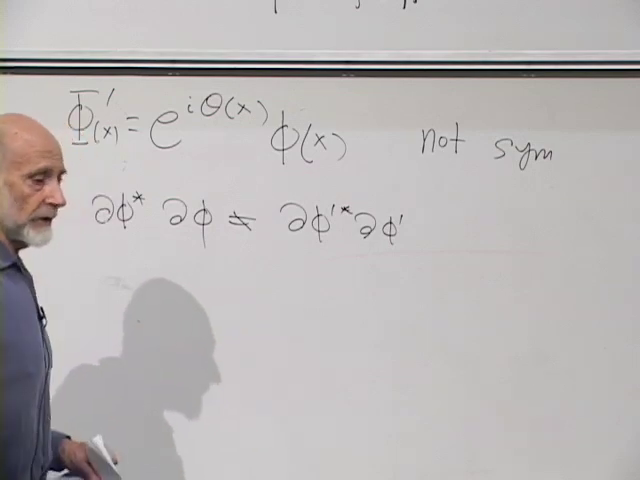
\includegraphics[width=0.78\textwidth]{lecture_08_figure_04.png}
\caption{Die Tafel hält die lokale Phasentransformation und das Versagen des gewöhnlichen Ableitungsterms, invariant zu bleiben, fest.}
\lectureframe{00:46:49}
\label{fig:l08-local-not-symmetry}
\end{figure}

Wir führen ein Vektorpotential ein und legen eine Konvention fest, die wir konsequent beibehalten:
\begin{equation}
  D_\mu=\partial_\mu+i g A_\mu,
  \qquad
  A_\mu'=A_\mu-\frac1g\partial_\mu\theta.
  \label{eq:l08-covariant-convention}
\end{equation}
Nun gilt
\begin{align}
  D_\mu'\phi'
  &=
  \left(\partial_\mu+i g A_\mu'\right)
  e^{i\theta}\phi
  \notag\\
  &=
  e^{i\theta}
  \left[
    \partial_\mu\phi+i(\partial_\mu\theta)\phi
    +i g A_\mu\phi-i(\partial_\mu\theta)\phi
  \right]
  \notag\\
  &=e^{i\theta}D_\mu\phi.
  \label{eq:l08-covariant-transform}
\end{align}
Die unerwünschten Terme heben sich auf. Die konjugierte Ableitung lautet
\begin{equation}
  (D_\mu\phi)^*
  =(\partial_\mu-i g A_\mu)\phi^*,
\end{equation}
und ihre entgegengesetzte Phase hebt sich im Produkt auf:
\begin{equation}
  (D_\mu\phi)^*D^\mu\phi.
\end{equation}

\begin{classroomqa}
\audiencequestion{War die Transformation des Eichfelds in der vorherigen Vorlesung mit umgekehrtem Vorzeichen angegeben?\lecturetimestamp{00:48:04}}
\lecturerresponse{Eine gleichzeitige Vorzeichenumkehr in \(D_\mu\) und im Transformationsgesetz ist lediglich eine Konvention. Bei \(D_\mu=\partial_\mu+i gA_\mu\) und \(\phi'=e^{i\theta}\phi\) muss für Konsistenz \(A_\mu'=A_\mu-g^{-1}\partial_\mu\theta\) gelten. Die alternative Konvention funktioniert ebenso gut, sofern alle Vorzeichen gemeinsam geändert werden.}
\end{classroomqa}

\begin{classroomqa}
\audiencequestion{Kennzeichnet die Verwendung einer Groß- oder Kleinbuchstabenform von \(\phi\) an der Tafel ein anderes Feld?\lecturetimestamp{00:55:02}}
\lecturerresponse{Nein, eine Unterscheidung ist nicht beabsichtigt. Die wechselnde Buchstabenform ist Handschrift, keine zusätzliche Operation und kein zweites Skalarfeld. Inhaltlich relevant sind der Strich, der Stern für die komplexe Konjugation und der Raumzeitindex.}
\end{classroomqa}

\begin{classroomqa}
\audiencequestion{Ist komplexe Konjugation dieselbe Operation wie das Heben oder Senken des Lorentz-Index im kinetischen Term?
\lecturetimestamp{00:56:50}}
\lecturerresponse{Nein. Der Stern komplex konjugiert das interne komplexe Feld. Lorentz-Indizes werden mit der Raumzeitmetrik gehoben:
\(D^\mu=g^{\mu\nu}D_\nu\). Ein Lorentz-Skalar erfordert die Kontraktion \((D_\mu\phi)^*D^\mu\phi\); beide Operationen kommen vor und erfüllen unterschiedliche Zwecke.}
\end{classroomqa}

\subsection{Das Eichfeld besitzt eine eigene Dynamik}

Der Feldstärketensor
\begin{equation}
  F_{\mu\nu}=\partial_\mu A_\nu-\partial_\nu A_\mu
  \label{eq:l08-field-strength}
\end{equation}
ist eichinvariant, weil sich die beiden gemischten zweiten Ableitungen von \(\theta\) aufheben. Seine Zeit--Raum-Komponenten enthalten das elektrische Feld, seine Raum--Raum-Komponenten das magnetische Feld. Die Elektrodynamik des Skalarfelds lautet daher
\begin{equation}
  \mathcal L
  =(D_\mu\phi)^*D^\mu\phi
  -V(\phi^*\phi)
  -\frac14F_{\mu\nu}F^{\mu\nu}.
  \label{eq:l08-abelian-higgs}
\end{equation}
Das geladene Feld ist hier bosonisch. Es ist nicht das Elektronenfeld, das ein Fermion ist. Ein geladener Heliumkern oder ein Cooper-Paar-Kondensat veranschaulicht, wie ein bosonischer geladener Freiheitsgrad entstehen kann.

Vor der Symmetriebrechung enthält der Eichterm Ableitungen von \(A_\mu\), aber keinen direkten Massenterm. Man könnte versuchen, \begin{equation}
  \frac12m_A^2A_\mu A^\mu,
\end{equation} hinzuzufügen, doch gemäß Gl. ~\eqref{eq:l08-covariant-convention} gilt
\begin{equation}
  A_\mu A^\mu
  \longmapsto
  \left(A_\mu-\frac1g\partial_\mu\theta\right)
  \left(A^\mu-\frac1g\partial^\mu\theta\right),
  \label{eq:l08-bare-mass-fails}
\end{equation}
was nicht gleich \(A_\mu A^\mu\) ist. Eine nackte Masse des Eichbosons ist durch die lokale Symmetrie verboten.

\begin{figure}[htbp]
\centering
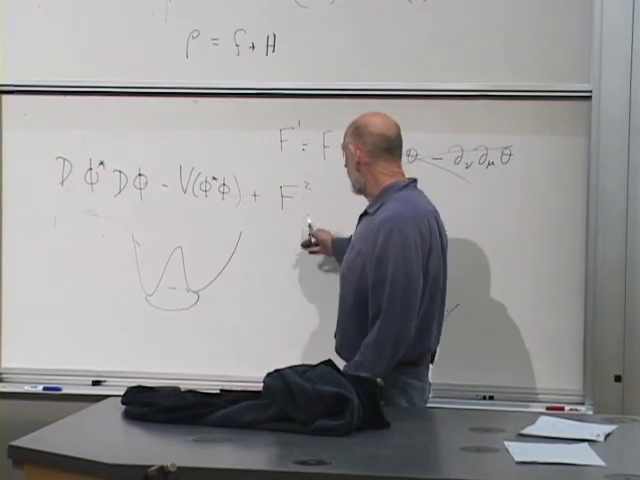
\includegraphics[width=0.76\textwidth]{lecture_08_figure_05.png}
\caption{Ein überprüfter Zustand der Tafel, der das Hindernis zeigt: Unter einer Eichtransformation wird \(A_\mu A^\mu\) zu einem Quadrat, das \(\partial_\mu\theta\) enthält; eine nackte Vektormasse ist daher nicht invariant.}
\lectureframe{01:07:30}
\label{fig:l08-bare-mass-board}
\end{figure}

\section{Der Higgs-Mechanismus}

\subsection{Die kovariante Ableitung erzeugt die Masse}

Wir kehren zum gebrochenen Potential zurück und verwenden die kanonisch normierte Parametrisierung
\begin{equation}
  \phi(x)=\frac{f+h(x)}{\sqrt2}
  e^{i\pi(x)/f}.
\end{equation}
Ihre kovariante Ableitung lautet
\begin{equation}
  D_\mu\phi
  =
  \frac{e^{i\pi/f}}{\sqrt2}
  \left[
    \partial_\mu h
    +i(f+h)
      \left(\frac{\partial_\mu\pi}{f}+gA_\mu\right)
  \right].
  \label{eq:l08-covariant-polar}
\end{equation}
Folglich gilt
\begin{equation}
\begin{aligned}
  (D_\mu\phi)^*D^\mu\phi
  ={}&
  \frac12(\partial_\mu h)^2
  \\
  &+\frac12(f+h)^2
    \left(\frac{\partial_\mu\pi}{f}+gA_\mu\right)
  \\
  &\hspace{4.2em}\times
    \left(\frac{\partial^\mu\pi}{f}+gA^\mu\right).
\end{aligned}
  \label{eq:l08-higgs-kinetic}
\end{equation}

Der entscheidende Term tritt bereits vor jeder Eichwahl auf:
\begin{equation}
  \frac12g^2f^2 A_\mu A^\mu.
  \label{eq:l08-vector-mass-term}
\end{equation}
Vergleichen wir ihn mit der Proca-Form \(\frac12m_A^2A_\mu A^\mu\), erhalten wir
\begin{equation}
  \boxed{m_A=g f}.
  \label{eq:l08-vector-mass}
\end{equation}
Dieselbe Entwicklung liefert auch die Wechselwirkungen \(g^2fh A_\mu A^\mu\) und \(\frac12g^2h^2A_\mu A^\mu\). Die Vektormasse ist also keine willkürliche Verletzung der Eichsymmetrie. Sie entsteht aus einem eichinvarianten kinetischen Skalarfeldterm, ausgewertet in einer Phase mit nicht verschwindendem Gleichgewichtsbetrag \(f\).

\begin{figure}[htbp]
\centering
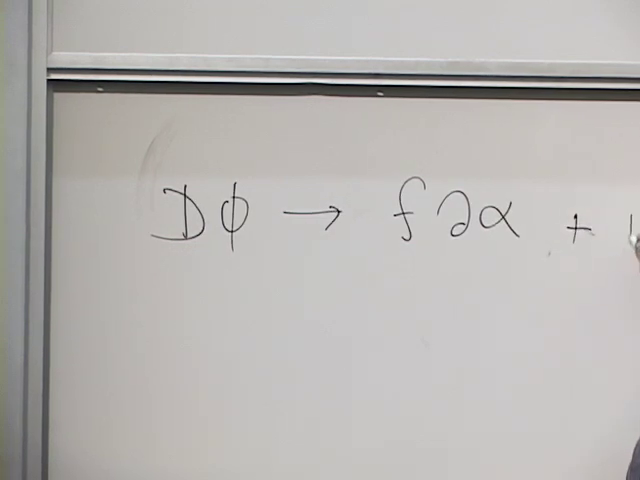
\includegraphics[width=0.78\textwidth]{lecture_08_figure_06.png}
\caption{Die Tafel isoliert den Beitrag \(f^2A^2\) innerhalb von \((D\phi)^*(D\phi)\). Numerische Faktoren hängen davon ab, wie das Skalarfeld und die Eichkopplung normiert sind; mit Gl. ~\eqref{eq:l08-canonical-polar} und \eqref{eq:l08-covariant-convention} ergibt sich \(m_A=gf\).}
\lectureframe{01:10:10}
\label{fig:l08-generated-mass-board}
\end{figure}

Die Vorlesung nimmt \(g\) und mehrere Faktoren von \(\sqrt2\) in ihre Tafelschreibweise auf. Daher wechselt sie bei der Bestimmung der Masse kurz zwischen \(f\), \(2f\) und \(\sqrt2f\). Diese Faktoren haben keine invariante Bedeutung, solange die Normierungen des kinetischen Terms und des Potentials nicht angegeben sind. Das robuste Ergebnis ist \(m_A\propto gf\); Gl. ~\eqref{eq:l08-vector-mass} gibt den Faktor für die hier verwendete Konvention an.

\subsection{Die Phase wird absorbiert}

Unter einer Eichtransformation ändert sich die Phasenvariable gemäß
\begin{equation}
  \pi'(x)=\pi(x)+f\,\theta(x).
\end{equation}
Wir wählen
\begin{equation}
  \theta(x)=-\frac{\pi(x)}{f}.
  \label{eq:l08-unitary-gauge-choice}
\end{equation}
Dann gilt \(\pi'=0\). Dies ist die unitäre Eichung, in der \begin{equation}
  \phi'(x)=\frac{f+h(x)}{\sqrt2}
\end{equation} reell ist, und Gl. ~\eqref{eq:l08-higgs-kinetic} vereinfacht sich zu
\begin{equation}
  (D_\mu\phi')^*D^\mu\phi'
  =
  \frac12(\partial_\mu h)^2
  +\frac12g^2(f+h)^2A_\mu'A^{\prime\mu}.
  \label{eq:l08-unitary-gauge-lagrangian}
\end{equation}
Das winkelabhängige Goldstone-Feld ist aus der Liste der unabhängigen Variablen verschwunden, während die Vektormasse erhalten bleibt.

Die Vorlesung zeigt dies zunächst im Grenzfall niedriger Energien \(\rho=f\), in dem
\begin{align}
  \phi&=f e^{i\alpha},
  \notag\\
  D_\mu\phi
  &=if e^{i\alpha}
    \left(\partial_\mu\alpha+gA_\mu\right),
  \notag\\
  (D_\mu\phi)^*
  &=-if e^{-i\alpha}
    \left(\partial_\mu\alpha+gA_\mu\right).
  \label{eq:l08-frozen-radius}
\end{align}
Ihr Produkt ist
\begin{equation}
  f^2
  \left(\partial_\mu\alpha+gA_\mu\right)
  \left(\partial^\mu\alpha+gA^\mu\right).
\end{equation}
Die Wahl \(\theta=-\alpha\) lässt \(g^2f^2A_\mu'A^{\prime\mu}\) übrig.

\begin{figure}[htbp]
\centering
\includegraphics[width=0.82\textwidth]{lecture_08_figure_07.png}
\caption{Der vollständige Tafelausdruck bei festgehaltenem Radius: Die kovarianten Ableitungen enthalten gemeinsam die Phasenableitung und das Vektorpotential. Als Nächstes wählt die Vorlesung \(\theta=-\alpha\), eliminiert dadurch die Phase und lässt den Vektormassenterm zurück.}
\lectureframe{01:16:20}
\label{fig:l08-frozen-radius-board}
\end{figure}

\begin{classroomqa}
\audiencequestion{Lässt sich die gesamte Lagrange-Funktion in Variablen umschreiben, die das Verschwinden des Winkelmodus explizit machen?
\lecturetimestamp{01:13:49}}
\lecturerresponse{Ja. In Polarkoordinaten tritt die Phase nur über die eichinvariante Kombination \(\partial_\mu\alpha+gA_\mu\) auf. Eine Eichtransformation mit \(\theta=-\alpha\) setzt die Phase überall dort auf null, wo diese Eichung wohldefiniert ist. Der kinetische Skalarfeldterm wird dann zu einem Vektormassenterm, während der eichinvariante Feldstärketerm unverändert bleibt.}
\end{classroomqa}

\begin{classroomqa}
\audiencequestion{Sind Schwingungen in \(\alpha\) nicht von Eichschwingungen zu unterscheiden?\lecturetimestamp{01:18:02}}
\lecturerresponse{In der geeichten Theorie ist eine reine Änderung von \(\alpha\), die durch die entsprechende Änderung von \(A_\mu\) kompensiert wird, eine Eich-Neubeschreibung und keine eigenständige physikalische Welle. Die invariante Größe ist \(\partial_\mu\alpha+gA_\mu\). Der physikalische Modus, der durch das globale Goldstone-Feld dargestellt wurde, tritt als longitudinale Polarisation des massiven Vektors wieder auf.}
\end{classroomqa}

Es ist üblich, von einer spontan gebrochenen lokalen Eichsymmetrie zu sprechen. Diese Ausdrucksweise ist in der Praxis nützlich: Nach einer Eichwahl hat das Skalarfeld einen von null verschiedenen Vakuumwert, und das Spektrum enthält einen massiven Vektor. Genau genommen verbinden Eichtransformationen jedoch redundante Beschreibungen und keine verschiedenen physikalischen Zustände.
\editorialnote{Eine lokale Eichredundanz ist nicht im selben eichinvarianten Sinn gebrochen wie eine globale Symmetrie. Präzise lautet die Aussage, dass sich die Theorie in einer Higgs-Phase befindet. Die eichfixierte Störungstheorie beschreibt diese Phase durch einen von null verschiedenen Erwartungswert des Skalarfelds und das daraus folgende Spektrum mit massivem Vektor.}

\section{Wohin der Goldstone-Freiheitsgrad ging}

Nichts Physikalisches kann allein dadurch verschwinden, dass wir die Variablen wechseln. Zählen wir die Freiheitsgrade vor und nach dem Übergang in die Higgs-Phase.

Vorher:
\begin{equation}
  \underbrace{2}_{\text{massless vector}}
  +
  \underbrace{2}_{\text{complex scalar}}
  =4.
\end{equation}
Ein masseloser Vektor hat zwei transversale Polarisationen. Das komplexe Skalarfeld hat zwei reelle Komponenten: eine radiale und eine winkelabhängige.

Nachher:
\begin{equation}
  \underbrace{3}_{\text{massive vector}}
  +
  \underbrace{1}_{\text{radial Higgs}}
  =4.
  \label{eq:l08-degree-count}
\end{equation}
Ein massiver Vektor lässt sich in sein Ruhesystem bringen. Dort ist keine räumliche Richtung ausgezeichnet, daher muss er drei Polarisationszustände besitzen. Bei Bewegung sind zwei davon transversal und einer longitudinal. Der Goldstone-Modus ist zu dieser longitudinalen Polarisation geworden.

\begin{figure}[htbp]
\centering
\begin{adjustbox}{max width=\linewidth}
\begin{tikzpicture}[x=1cm,y=1cm]
  \node[draw,rounded corners,fill=blue!7,minimum width=4.3cm,
        minimum height=2.1cm,align=center] (before) at (0,0)
    {massless \(A_\mu\): \(2\) transverse\\
     \(+\)\\
     complex \(\phi\): \(h+\pi\)};
  \node[draw,rounded corners,fill=orange!10,minimum width=4.3cm,
        minimum height=2.1cm,align=center] (after) at (7,0)
    {massive \(A_\mu\): \(2\) transverse\\
     \(+\;1\) longitudinal\\
     \(+\) radial \(h\)};
  \draw[->,very thick] (before) -- node[above]{Higgs phase} (after);
  \draw[->,teal!70!black,thick]
    (-0.15,-0.65) to[bend right=28]
    node[below,align=center]{Goldstone \(\pi\) supplies\\longitudinal mode}
    (6.8,-0.65);
\end{tikzpicture}
\end{adjustbox}
\caption{Der Higgs-Mechanismus ordnet die physikalischen Freiheitsgrade neu, statt sie zu vernichten.}
\label{fig:l08-degree-rearrangement}
\end{figure}

\begin{classroomqa}
\audiencequestion{Wie kann der winkelabhängige Freiheitsgrad verschwinden, ohne die Zählung der Freiheitsgrade zu verletzen?\lecturetimestamp{01:19:13}}
\lecturerresponse{Physikalisch verschwindet er nicht. Ein masseloser Vektor hat zwei Helizitäten, weil er nicht in sein Ruhesystem gebracht werden kann. Ein massiver Vektor hat drei Polarisationen, darunter eine longitudinale. Der Goldstone-Modus wird zu dieser dritten Polarisation, sodass die Gesamtzahl unverändert bleibt.}
\end{classroomqa}

Die Vorlesung bietet einen nützlichen kinematischen Test. Man stelle sich ein massives Vektorteilchen vor, bremse es bis zum Stillstand ab und beschleunige es in eine neue Richtung. Eine Polarisation, die bezüglich der ursprünglichen Bewegungsrichtung transversal war, kann bezüglich der neuen Richtung longitudinal werden. Ebenso kehrt sich die Helizitätsbezeichnung um, wenn ein zirkular polarisiertes massives Teilchen durch den Ruhezustand gebracht und in die entgegengesetzte Richtung geschickt wird. Ein streng masseloses Teilchen kann dieses Experiment nicht durchlaufen, denn kein Inertialsystem kann es zum Stillstand bringen. Seine beiden Helizitäten bilden daher ein konsistentes physikalisches Spektrum.

\section{Das Analogon im Supraleiter}

In einem herkömmlichen Supraleiter bilden Elektronen Cooper-Paare. Ein Paar ist ein Boson mit elektrischer Ladung \(2e\), und das Kondensat wird durch einen geladenen komplexen Ordnungsparameter beschrieben. Ist sein Betrag ungleich null, erzeugt die Kombination aus seiner Phase und dem elektromagnetischen Vektorpotential den Anderson--Higgs-Mechanismus. Statische Magnetfelder klingen über die London-Eindringtiefe ab, statt sich frei durch das Volumen auszubreiten. In diesem präzisen, vom Medium abhängigen Sinn verhält sich das Photon, als hätte es Masse erhalten.

Dieses Beispiel verdeutlicht auch die anfängliche Unterscheidung. Das elektromagnetische Feld wird nicht dauerhaft in ein anderes Elementarteilchen umgewandelt. Das massive Ausbreitungsgesetz gilt für den kollektiven Zustand im Inneren des Materials; außerhalb bleibt das Photon im Vakuum masselos.

\section{Was gezeigt wurde}

Das Argument lässt sich nun zusammenfassen, ohne seine Logik zu verlieren:
\begin{enumerate}
  \item Eine gebrochene globale kontinuierliche Symmetrie besitzt eine flache Winkelrichtung und daher einen masselosen Goldstone-Modus.
  \item Lokale Phaseninvarianz erfordert ein Eichpotential und ersetzt \(\partial_\mu\) durch \(D_\mu\).
  \item Eine nackte Masse für \(A_\mu A^\mu\) verletzt das lokale Transformationsgesetz.
  \item Besitzt das geladene Skalarfeld einen von null verschiedenen Gleichgewichtsbetrag \(f\), enthält der eichinvariante Term \(|D_\mu\phi|^2\) den Beitrag \(\frac12g^2f^2A_\mu A^\mu\).
  \item Die Phase lässt sich durch eine Eichwahl entfernen, und ihr physikalischer Freiheitsgrad wird zur longitudinalen Polarisation des massiven Vektors.
  \item Die radiale Higgs-Anregung bleibt erhalten; ihre Masse wird durch die Krümmung des Skalarfeldpotentials festgelegt.
\end{enumerate}

Als Nächstes müssen wir Fermionen ihre Massen verleihen. Elektronen und Quarks können den Vektormechanismus nicht direkt nutzen; ihre Kopplungen an das Higgs-Feld sind Yukawa-Wechselwirkungen. Sobald sich das Skalarfeld bei \(f\) einpendelt, werden diese Wechselwirkungen zu Fermionmassentermen.

Die allgemeine Aussage, dass vertraute Teilchen ohne elektroschwache Symmetriebrechung masselos wären, bedarf noch einer letzten Einschränkung. Die Massen der elementaren Quarks und geladenen Leptonen sowie die Massen von \(W\) und \(Z\) verschwinden tatsächlich mit dem Higgs-Erwartungswert. Der größte Teil der Protonen- und Neutronenmasse entsteht jedoch dynamisch durch QCD-Confinement und die Energie des starken Feldes, nicht durch die Higgs-Massen der Quarks. Diese Unterscheidung ändert nichts am hier hergeleiteten Higgs-Mechanismus; sie grenzt seinen Anwendungsbereich präzise ab.

\chapter{Fermionenmassen: Chiralität, Yukawa-Kopplungen und Majorana-Neutrinos}

\lectureoverview{Zunächst rekonstruieren wir den Higgs-Mechanismus für Eichbosonen in einer Spielzeugtheorie \(U(1)\) und stellen dann die entsprechende Frage für Fermionen. Eine Dirac-Masse mischt links- und rechtsh chirale Felder, doch die schwache Wechselwirkung weist ihnen unterschiedliche Ladungen zu und verbietet deshalb eine nackte Masse. Eine Yukawa-Kopplung an das Higgsfeld respektiert die Symmetrie; sobald das Higgsfeld einen Vakuumerwartungswert annimmt, wird dieselbe Wechselwirkung zu einer Fermionenmasse und zu einer messbaren Higgs--Fermion-Kopplung. Im letzten Teil verfolgen wir diese Logik weiter zu Neutrinomassen, möglichen schweren, ungeschützten Teilchen, kosmischer Strahlung, relativistischer Trägheit und Gravitation.}

Die einleitende Wiederholung soll nicht einfach nur die vorherige Vorlesung wiederholen. Wir brauchen daraus eine Idee in einer Form, die sich auf Fermionen übertragen lässt: Eine Masse entspricht einer von null verschiedenen Energie für eine Anregung bei verschwindendem Impuls. Bei einem Feld bedeutet verschwindender Impuls unendliche Wellenlänge oder eine Verschiebung, die überall gleich ist. Eine Theorie, deren Terme nur Ableitungen enthalten, kann eine gleichförmige Verschiebung nicht erfassen. Ein Term ohne Ableitungen kann das.

\section{Die Geschichte der Eichbosonen in einem Zug}

\subsection{Ableitungsenergie und ein masseloser Vektor}

Das Eichfeld des Modells ist \(A_\mu\), mit der Feldstärke
\begin{equation}
  F_{\mu\nu}
  =\partial_\mu A_\nu-\partial_\nu A_\mu .
  \label{eq:l09-field-strength}
\end{equation}
An der Tafel wird der kinetische Term des Eichfelds schematisch als \(F^2\) angeschrieben. Bei einer üblichen Normierung lautet er
\begin{equation}
  \mathcal L_{\mathrm{gauge}}
  =-\frac14 F_{\mu\nu}F^{\mu\nu}.
  \label{eq:l09-gauge-kinetic}
\end{equation}

\begin{figure}[htbp]
\centering
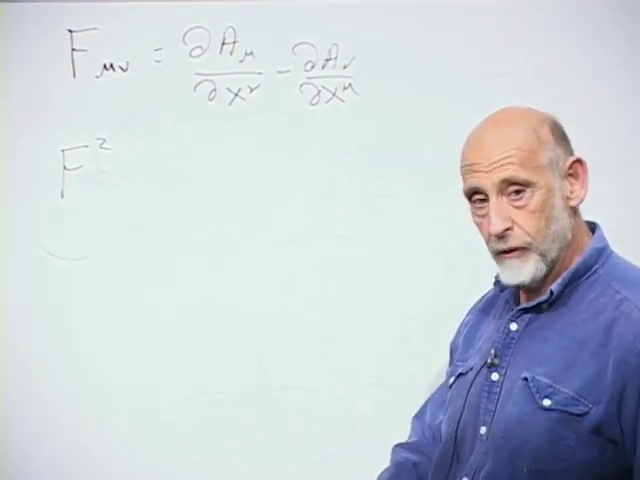
\includegraphics[width=0.72\textwidth]{lecture_09_figure_02.png}
\caption{Definition der Feldstärke und die an der Tafel verwendete Kurzschreibweise \(F^2\) für die Ableitungsenergie des Eichfelds.}
\lectureframe{00:02:39}
\label{fig:l09-field-strength-board}
\end{figure}

Jedes Auftreten von \(A_\mu\) in \eqref{eq:l09-gauge-kinetic} steht unter einer Ableitung. Daher verändert
\begin{equation}
  A_\mu(x)\longmapsto A_\mu(x)+c_\mu,
  \qquad \partial_\nu c_\mu=0,
\end{equation}
\(F_{\mu\nu}\) nicht. Ein homogenes Vektorpotential verursacht folglich keine Feldstärkeenergie. In der Sprache der Vorlesung hat die Mode bei verschwindendem Impuls keine Lücke, und das Eichboson ist masselos.

Dieses \(U(1)\)-Feld ist ein bewusst einfach gehaltener Stellvertreter. Das physikalische Ziel sind \(W^\pm\) und \(Z\), nicht das Photon der Elektromagnetischen Wechselwirkung. Die ungebrochene elektromagnetische Symmetrie lässt das Photon masselos; die gebrochene elektroschwache Symmetrie verleiht den schwachen Eichbosonen eine Masse.

\subsection{Den radialen Freiheitsgrad des Higgsfelds einfrieren}

Führen wir ein geladenes komplexes Skalarfeld ein und schreiben es in Polarkoordinaten:
\begin{equation}
  \phi(x)=\rho(x)e^{i\alpha(x)}.
\end{equation}
Sein mexikanisches-Hut-Potential hat sein Minimum auf einem Kreis mit endlichem Radius. Bezeichnen wir diesen Radius mit \(f\), so ist die radiale Richtung vergleichsweise steif. Für die erste Betrachtung frieren wir sie ein und behalten nur die Phase:
\begin{equation}
  \phi(x)\simeq f e^{i\alpha(x)}.
  \label{eq:l09-frozen-higgs}
\end{equation}

\begin{figure}[htbp]
\centering
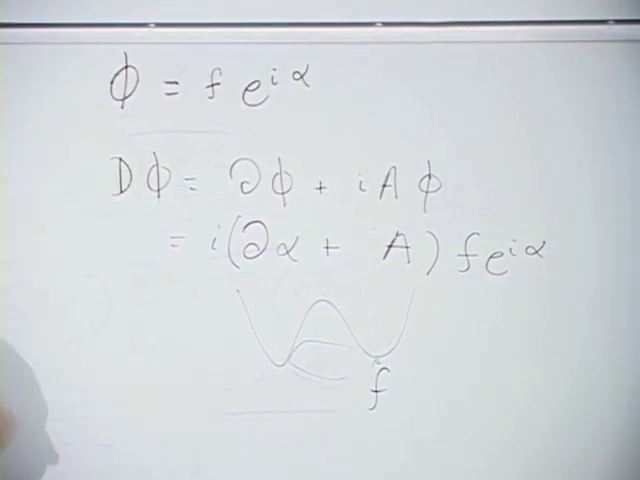
\includegraphics[width=0.72\textwidth]{lecture_09_figure_03.png}
\caption{Der eingefrorene Radius des Higgsfelds, seine kovariante Ableitung und die kleine Skizze des gebrochenen Potentials aus der Wiederholung.}
\lectureframe{00:06:42}
\label{fig:l09-frozen-board}
\end{figure}

Wählen wir die Konvention
\begin{equation}
\begin{aligned}
  D_\mu&=\partial_\mu+igA_\mu,
  \\
  \phi&\longmapsto e^{i\theta}\phi,
  \\
  A_\mu&\longmapsto A_\mu-\frac1g\partial_\mu\theta .
\end{aligned}
  \label{eq:l09-gauge-convention}
\end{equation}
In der Vorlesung wird \(g\) unterdrückt; wenn wir es sichtbar lassen, werden die Dimensionen und die spätere Masse deutlich. Auf das eingefrorene Feld angewandt ergibt sich
\begin{align}
  D_\mu\phi
  &=(\partial_\mu+igA_\mu)f e^{i\alpha}
  \notag\\
  &=i\bigl(\partial_\mu\alpha+gA_\mu\bigr)
    f e^{i\alpha}.
  \label{eq:l09-covariant-frozen}
\end{align}
Die Multiplikation mit der komplex konjugierten Größe beseitigt die Phase und macht außerdem aus \(i\) mal \(-i\) den Faktor \(+1\):
\begin{equation}
  |D_\mu\phi|^2
  =f^2
   \bigl(\partial_\mu\alpha+gA_\mu\bigr)
   \bigl(\partial^\mu\alpha+gA^\mu\bigr).
  \label{eq:l09-frozen-square}
\end{equation}

\begin{classroomqa}
\audiencequestion{Müsste beim Quadrat der kovarianten Ableitung ein Minuszeichen stehen, weil die Ableitung den Faktor \(i\) ergibt?
\lecturetimestamp{00:07:39}}
\lecturerresponse{Nein. Der kinetische Term ist das Produkt mit der komplex konjugierten Größe. Ein Faktor liefert \(i\), der andere \(-i\), und \(i(-i)=1\). Die Vorzeichenkonvention für \(D_\mu\) kann konsistent umgekehrt werden; der Betragsquadratterm ist jedoch im entsprechenden Energieausdruck positiv.}
\end{classroomqa}

Die Kombination in \eqref{eq:l09-frozen-square} ist selbst ein verschobenes Eichfeld. Wählen wir \(\theta=-\alpha\), sodass die Phase des Skalarfelds verschwindet, und definieren wir
\begin{equation}
  A'_\mu=A_\mu+\frac1g\partial_\mu\alpha .
  \label{eq:l09-unitary-gauge-field}
\end{equation}
Dann gilt
\begin{equation}
  |D_\mu\phi|^2=g^2f^2 A'_\mu A'^\mu .
  \label{eq:l09-vector-mass-term}
\end{equation}
Der neue Term enthält keine Ableitung von \(A'_\mu\). Ein homogenes Feld trägt nun Energie, sodass die Vektormode bei verschwindendem Impuls eine Lücke hat.

\begin{figure}[htbp]
\centering
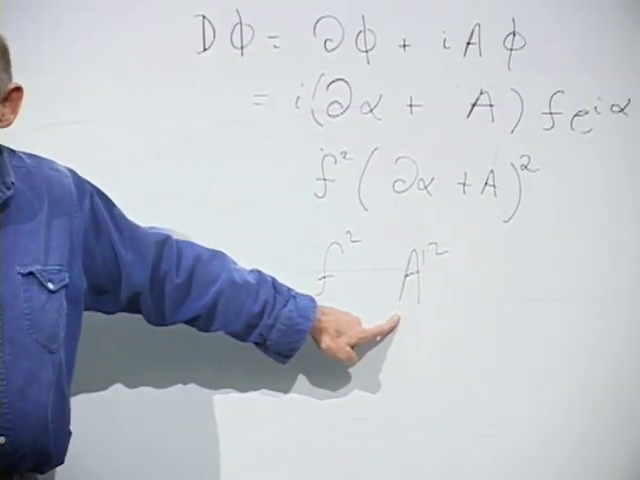
\includegraphics[width=0.72\textwidth]{lecture_09_figure_04.png}
\caption{An der Tafel wird der Term \(f^2A^2\) herausgestellt, der nach Absorption der Phase auf eine Masse des Eichbosons hinweist.}
\lectureframe{00:10:31}
\label{fig:l09-vector-mass-board}
\end{figure}

Bei kanonischer Normierung des Skalarfelds schreibt man
\(\phi=(f+h)e^{i\pi/f}/\sqrt2\). Der Vergleich des resultierenden Vektorterms mit
\(\tfrac12m_A^2A_\mu A^\mu\) ergibt
\begin{equation}
  m_A=gf
  \label{eq:l09-abelian-vector-mass}
\end{equation}
in diesem abelschen Modell. In der Vorlesung werden die Normierungsfaktoren unterdrückt und das Ergebnis mit der Aussage zusammengefasst, dass die Vektormasse durch \(f\) bestimmt wird.

Die Phasenmode ist nicht einfach verschwunden. Vor der Eichung war sie ein masseloses Goldstone-Boson. Nach der Eichung liefert sie die longitudinale Polarisation, die ein massives Vektorteilchen benötigt. Die radiale Fluktuation, die wir vorübergehend eingefroren haben, bleibt als physikalische Higgs-Anregung erhalten.

\subsection{Warum ein Term ohne Ableitungen Masse bedeutet}

\begin{classroomqa}
\audiencequestion{Warum zählt ein Term \(A'^2\) als Masse und nicht einfach als eine weitere Wechselwirkung?\lecturetimestamp{00:13:10}}
\lecturerresponse{Masse ist Ruheenergie. Bei einem Feld ist ein Teilchen in Ruhe das Quant einer Mode mit verschwindendem Impuls und unendlicher Wellenlänge. Der Ableitungsterm liefert einer statischen homogenen Verschiebung keine Energie, \(m_A^2A'^2\) dagegen schon. Diese von null verschiedene Energie bei verschwindendem Impuls ist die Ruheenergielücke.}
\end{classroomqa}

Die Vorlesung erläutert diese Aussage anhand dreier mechanischer Analogien.

\begin{itemize}
  \item In einem Kristall kostet eine langsam variierende Verschiebung elastische Energie, weil benachbarte Atome unterschiedlich verschoben werden. Eine starre Translation verschiebt alle Atome gemeinsam und kostet keine innere Energie. Das akustische Phonon ist daher lückenlos.
  \item In einem idealen rotationssymmetrischen Magneten kostet eine räumlich variierende Spinrichtung Austauschenergie, eine gemeinsame Drehung aller Spins dagegen nicht. Die zugehörige langwellige Spinwelle ist lückenlos.
  \item In einem Plasma erzeugt eine Verschiebung des Elektronenfluids relativ zum positiven Hintergrund eine Ladungstrennung und ein rücktreibendes elektrisches Feld, selbst bei einer homogenen Relativverschiebung. Das daraus entstehende Plasmon hat bei verschwindender Wellenzahl eine von null verschiedene Frequenz.
\end{itemize}

Das mit dem Higgsmechanismus versehene Eichfeld verhält sich wie das dritte Beispiel: Das gebrochene Medium widersetzt sich einer homogenen Verschiebung, die andernfalls keine Energie kosten würde.

\begin{classroomqa}
\audiencequestion{Hat die Phase \(\alpha\) nicht schon vor Einführung des Eichfelds geschwungen?\lecturetimestamp{00:18:24}}
\lecturerresponse{Doch. Ihre Energie war proportional zu \(f^2(\partial_\mu\alpha)^2\). Eine räumlich variierende Phase hat Gradientenenergie und kann sich ausbreiten; eine gleichförmige Phasenänderung kostet jedoch nichts. Genau das ist die masselose Goldstone-Mode.}
\end{classroomqa}

\begin{classroomqa}
\audiencequestion{Die Ableitung enthält auch eine Zeitableitung. Hat die tatsächliche Bewegung des gesamten Gitters oder die Änderung des gesamten Felds dann keine kinetische Energie?\lecturetimestamp{00:22:18}}
\lecturerresponse{Doch. Verglichen werden statische Konfigurationen oder solche, die beliebig langsam vorbereitet werden. Ein Gitter, das sich mit endlicher Geschwindigkeit verschiebt, hat kinetische Energie. Beim Massentest wird gefragt, ob die Konfiguration auch dann Energie hat, wenn sie in Ruhe und räumlich homogen ist.}
\end{classroomqa}

\section{Der experimentelle Hinweis: Die schwache Wechselwirkung unterscheidet links und rechts}

Nun wendet sich die Vorlesung dem Elektron, dem Myon und den Quarks zu. Auch ihre Massen entstehen durch das Higgsfeld, doch der Mechanismus sieht anders aus, weil eine Fermionenmasse kein quadratischer Vektorterm ist. Sie koppelt zwei chirale Felder miteinander.

\subsection{Paritätsverletzung beim Betazerfall}

Ausgangspunkt ist der empirische Befund, dass die schwache Wechselwirkung die Parität verletzt. Die Quantenelektrodynamik und die Quantenchromodynamik behandeln einen Prozess und sein Spiegelbild gleich. Die schwache Wechselwirkung tut das nicht. Beim Betazerfall des Neutrons,
\begin{equation}
  n\longrightarrow p+e^-+\bar\nu_e,
  \label{eq:l09-beta-decay}
\end{equation}
haben die energiereichen Elektronen, die durch die geladene Stromwechselwirkung ausgewählt werden, linkshändige Helizität: Ihr Spin zeigt entgegengesetzt zu ihrem Impuls. Die entsprechenden Antineutrinos haben die entgegengesetzte Helizität.

Für ein ultrarelativistisches Teilchen definieren wir die Helizität durch
\begin{equation}
  h=\frac{\bm S\cdot\bm p}{|\bm S|\,|\bm p|}.
\end{equation}
Spin parallel zum Impuls entspricht \(h=+1\); Spin antiparallel dazu entspricht \(h=-1\). Die schwache Wechselwirkung koppelt an ein linkschirales Elektronenfeld und ein linkschirales Neutrinofeld, nicht in gleicher Weise an ein rechtschirales Elektronenfeld.\editorialnote{Die Vorlesung verwendet zunächst Händigkeit im Sinne der Helizität, weil sie bei hohen Energien anschaulich ist. Eichladungen wirken tatsächlich auf die Chiralität, also auf das Lorentz-Darstellungslabel, das durch \(P_L=(1-\gamma^5)/2\) und \(P_R=(1+\gamma^5)/2\) ausgewählt wird. Bei einem masselosen Teilchen stimmen Chiralität und Helizität für Teilchen überein; bei einem massiven Teilchen ist das nicht der Fall.}

Um das Hindernis ohne die vollständige Buchführung für \(SU(2)_L\times U(1)_Y\) sichtbar zu machen, stellen wir uns eine fiktive Welt mit \(U(1)\) vor, in der nur \(\psi_L\) die betreffende Ladung trägt:
\begin{equation}
  \psi_L\longmapsto e^{i\theta}\psi_L,
  \qquad
  \psi_R\longmapsto\psi_R .
  \label{eq:l09-chiral-toy-charge}
\end{equation}
Das ist nicht Elektromagnetismus: Reale links- und rechtschirale Elektronen tragen dieselbe elektrische Ladung. Es ist eine Karikatur der schwachen Wechselwirkung, bei der die beiden Chiralitäten zu unterschiedlichen elektroschwachen Darstellungen gehören.

\begin{classroomqa}
\audiencequestion{Gilt dieselbe Links--Rechts-Asymmetrie auch für Quarks?
\lecturetimestamp{00:31:50}}
\lecturerresponse{Ja, mit den entsprechenden schwachen Multipletts und Hyperladungen. LinksChirale Up- und Down-Quarks bilden schwache Dubletts, während die rechtschiralen Felder schwache Singuletts sind. Ihre Higgs-Kopplungen stehen deshalb vor demselben strukturellen Problem wie die des Elektrons.}
\end{classroomqa}

\section{Eine Dirac-Masse mischt links--rechts}

\subsection{Von der Vierkomponentengleichung zu zwei Weyl-Gleichungen}

Eine Dirac-Wellenfunktion hat vier Komponenten. Grob gesagt beschreiben zwei davon den Spin, während zwei zwischen Lösungen positiver und negativer Energie unterscheiden; Letztere werden als Freiheitsgrade der Antiteilchen interpretiert. In Hamilton-Form lautet die Gleichung
\begin{equation}
  i\frac{\partial\Psi}{\partial t}
  =\left(-i\bm\alpha\cdot\bm\nabla+m\beta\right)\Psi .
  \label{eq:l09-dirac-hamiltonian}
\end{equation}
Die Matrizen \(\alpha_i\) und \(\beta\) kodieren den relativistischen Zusammenhang zwischen Energie, Impuls und Masse.

\begin{figure}[htbp]
\centering
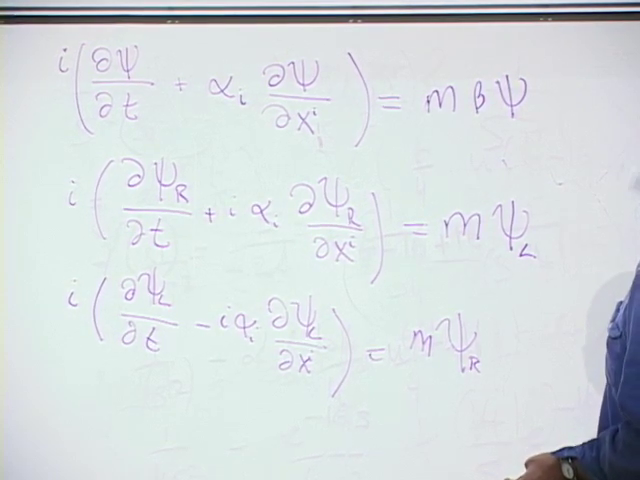
\includegraphics[width=0.74\textwidth]{lecture_09_figure_05.png}
\caption{An der Tafel wird zunächst die Dirac-Gleichung angeschrieben und dann in gekoppelte Gleichungen für links- und rechtshändige Anteile aufgespalten.}
\lectureframe{00:40:30}
\label{fig:l09-dirac-board}
\end{figure}

In der chiralen Basis wird die Rolle von \(m\) deutlich. Mit
\(\sigma^\mu=(1,\bm\sigma)\) und
\(\bar\sigma^\mu=(1,-\bm\sigma)\) gilt
\begin{align}
  i\bar\sigma^\mu\partial_\mu\psi_L&=m\psi_R,
  \label{eq:l09-weyl-left}\\
  i\sigma^\mu\partial_\mu\psi_R&=m\psi_L.
  \label{eq:l09-weyl-right}
\end{align}
Für \(m=0\) sind die Gleichungen unabhängig: Ein links- und ein rechtschirales Feld können sich ausbreiten, ohne miteinander zu wechselwirken. Für \(m\neq0\) tritt jedes der beiden als Quelle des anderen auf. Genau das bedeutet es, dass eine Dirac-Masse links und rechts mischt.

Susskind beschreibt dies als ein Oszillieren des Fermions zwischen links und rechts. Diese Formulierung erfasst die Kopplung, sollte aber nicht als wörtliches klassisches Bild eines Punktteilchens verstanden werden, das hin und her kippt. Die präzise Aussage steckt in der gekoppelten Feldgleichung \eqref{eq:l09-weyl-left}--\eqref{eq:l09-weyl-right}.

\begin{classroomqa}
\audiencequestion{Sind die Faktoren \(i\) und die Vorzeichen in den beiden Gleichungen an der Tafel konsistent?\lecturetimestamp{00:41:10}}
\lecturerresponse{Nicht Zeile für Zeile an der Tafel: Bei der schnellen Herleitung wurde ein \(i\) inkonsistent ausgeklammert. Verlässlich ist das Kopplungsmuster. Die Gleichungen \eqref{eq:l09-weyl-left} und \eqref{eq:l09-weyl-right} entsprechen einer üblichen konsistenten Konvention.}
\end{classroomqa}

\subsection{Warum die schwache Symmetrie eine nackte Masse verbietet}

Der entsprechende Dirac-Massenterm in der Lagrange-Dichte lautet
\begin{equation}
  \mathcal L_m
  =-m\bar\psi\psi
  =-m\left(\bar\psi_L\psi_R+\bar\psi_R\psi_L\right).
  \label{eq:l09-bare-dirac-mass}
\end{equation}
Unter der Spielzeugtransformation \eqref{eq:l09-chiral-toy-charge} gilt
\begin{equation}
  \bar\psi_L\psi_R\longmapsto
  e^{-i\theta}\bar\psi_L\psi_R,
  \qquad
  \bar\psi_R\psi_L\longmapsto
  e^{i\theta}\bar\psi_R\psi_L.
\end{equation}
Keiner der beiden Terme ist invariant. Der direkte Koeffizient \(m\) für die Links--Rechts-Mischung ist daher vor der Symmetriebrechung verboten.

Der Elektromagnetismus allein würde dieses Problem nicht verursachen, denn \(\psi_L\) und \(\psi_R\) haben dieselbe elektrische Ladung. Das Hindernis entsteht durch ihre unterschiedlichen schwachen Quantenzahlen.

\subsection{Helizitätsfragen, die die Feinheiten der Chiralität sichtbar machen}

Nun prüft der Kurs das anschauliche Bild der Händigkeit aus mehreren Blickwinkeln. Diese Fragen sind keine Nebensache: Sie zeigen genau, wo die Helizität hilfreich ist und wo man stattdessen die Chiralität heranziehen muss.

\begin{classroomqa}
\audiencequestion{Wie sähe die Welt aus, wenn die schwache Wechselwirkung Elektronen mit beiden Helizitäten gleich häufig emittierte?\lecturetimestamp{00:42:12}}
\lecturerresponse{Die unmittelbare Paritätsasymmetrie in diesem Prozess wäre dann nicht vorhanden. Die reale elektroschwache Theorie ist jedoch chiral: Nur die linkschiralen Dubletts tragen die geladene schwache Wechselwirkung. Die Vorlesung verschiebt eine ausführlichere Erklärung dafür, warum die Natur diese Struktur gewählt hat, auf später.}
\end{classroomqa}

\begin{classroomqa}
\audiencequestion{Angenommen, der Spin eines Elektrons wird vertikal präpariert und das Elektron anschließend horizontal beschleunigt. Ist es links- oder rechtshändig?
\lecturetimestamp{00:42:44}}
\lecturerresponse{Ein Spin-Zustand, der quer zum Impuls steht, ist eine Überlagerung der beiden Helizitäten. Eine scharfe Helizität liegt nur vor, wenn der Spin parallel oder antiparallel zum Impuls ist. Die chiralen Projektoren der schwachen Wechselwirkung sind für das Feld dennoch wohldefiniert.}
\end{classroomqa}

Ein massives Teilchen kann bis zum Stillstand abgebremst und in die entgegengesetzte Richtung beschleunigt werden, ohne seinen Spin umzudrehen. Dabei ändert seine Helizität das Vorzeichen. Ein masseloses Teilchen kann durch einen Lorentz-Boost weder überholt noch zum Stillstand gebracht werden; seine Helizität bleibt daher unter eigentlichen Boosts invariant. Das motiviert die Aussage der Vorlesung, dass eine Teilchensorte mit nur einer physikalischen Helizität masselos sein muss. Präziser lautet die feldtheoretische Aussage: Eine Lorentz-invariante Dirac-Masse erfordert beide Chiralitäten.

\begin{classroomqa}
\audiencequestion{Ein zirkular polarisiertes Photon kann an einem Spiegel reflektiert werden und seine Ausbreitungsrichtung umkehren, ohne jemals zum Stillstand zu kommen. Widerspricht das dem Helizitätsargument?
\lecturetimestamp{00:45:28}}
\lecturerresponse{Nein. Der Spiegel ist ein äußeres System, das Drehimpuls austauschen und die Ausbreitungsrichtung umkehren kann. Eine Reflexion ist kein Lorentz-Boost, der das Photon überholt. Ob ein Kanal existiert, hängt außerdem von den erlaubten Polarisationszuständen und den Randbedingungen des Materials ab.}
\end{classroomqa}

\begin{classroomqa}
\audiencequestion{Enthält ein gewöhnlicher Elektronenstrahl eine oder beide Händigkeiten?
\lecturetimestamp{00:46:10}}
\lecturerresponse{Im Allgemeinen beide. Ein Zustand eines massiven Elektrons enthält beide chiralen Komponenten, und ein unpolarisierter Strahl enthält beide Helizitäten. Spezielle Quellen können einen polarisierten Strahl mit einer starken Helizitätsasymmetrie erzeugen.}
\end{classroomqa}

\begin{classroomqa}
\audiencequestion{Kann ein Strahl unabhängig vom Spin fokussiert werden, oder trennen Magnetfelder die beiden Polarisationen?
\lecturetimestamp{00:46:29}}
\lecturerresponse{Eine gewöhnliche Ortsfokussierung kann weitgehend spinunabhängig sein, doch magnetische Momente koppeln an Gradienten des Magnetfelds. Spinselektive Quellen, Stern--Gerlach-artige Gradienten und die Spindynamik im Beschleuniger können daher Polarisationen präparieren oder voneinander trennen.}
\end{classroomqa}

\begin{classroomqa}
\audiencequestion{Ist der Unterschied zwischen links und rechts bei der schwachen Wechselwirkung bloß Zufall?
\lecturetimestamp{00:48:13}}
\lecturerresponse{Im Rahmen dieses Kurses ist er ein experimenteller Befund, der im Standardmodell verankert ist. Er ist so systematisch, dass er kaum wie ein beiläufiger Zufall wirkt; doch das Standardmodell selbst leitet das vollständige Muster der chiralen Ladungen nicht aus einem tieferen Prinzip her.}
\end{classroomqa}

\section{Die Yukawa-Konstruktion}

\subsection{Das Higgsfeld die fehlende Ladung tragen lassen}

Die Symmetrie verbietet eine numerische Masse, erlaubt aber eine Wechselwirkung mit einem Feld, das die fehlende Transformationsphase beisteuert. Führen wir ein komplexes Skalarfeld ein mit
\begin{equation}
  \phi\longmapsto e^{i\theta}\phi,
  \qquad
  \phi^\dagger\longmapsto e^{-i\theta}\phi^\dagger.
  \label{eq:l09-scalar-charge}
\end{equation}
Dann ist
\begin{equation}
  \mathcal L_Y
  =-y\,\bar\psi_L\phi\psi_R
   -y^*\,\bar\psi_R\phi^\dagger\psi_L
  \label{eq:l09-yukawa-lagrangian}
\end{equation}
eichinvariant. Im ersten Term trägt \(\bar\psi_L\) den Faktor \(e^{-i\theta}\) bei und \(\phi\) den Faktor \(e^{i\theta}\); die Phasen heben sich auf. Der zweite Term ist die hermitesch konjugierte Größe.

Entsprechend erhalten die chiralen Gleichungen eine feldabhängige Mischung:
\begin{align}
  i\bar\sigma^\mu D_\mu\psi_L
    &=y\phi\psi_R,
  \label{eq:l09-yukawa-eom-left}\\
  i\sigma^\mu\partial_\mu\psi_R
    &=y^*\phi^\dagger\psi_L.
  \label{eq:l09-yukawa-eom-right}
\end{align}

\begin{figure}[htbp]
\centering
\includegraphics[width=0.76\textwidth]{lecture_09_figure_06.png}
\caption{Die nackte Masse auf den rechten Seiten wurde durch das geladene Skalarfeld ersetzt. Die genauen Vorzeichen an der Tafel sind schematisch; die invariante Struktur steht in \eqref{eq:l09-yukawa-lagrangian}.}
\lectureframe{00:51:30}
\label{fig:l09-yukawa-board}
\end{figure}

Vor der Symmetriebrechung handelt es sich hierbei um eine Wechselwirkung und nicht um eine Masse. Ein rechtschirales Fermion kann nur dann in ein linkschirales Fermion übergehen, wenn es das Skalarquant emittiert oder absorbiert, das zum Ausgleich der Ladung erforderlich ist. Der Koeffizient \(y\) ist eine Yukawa-Kopplung und nicht die Eichladung \(g\).

\begin{classroomqa}
\audiencequestion{Ist es zulässig, einfach \(\phi\) und \(\phi^\dagger\) auf die rechten Seiten der beiden Gleichungen zu setzen?
\lecturetimestamp{00:51:55}}
\lecturerresponse{Das ist genau deshalb zulässig, weil ihre Transformationsphasen die Abweichung ausgleichen. Entscheidend ist nicht die äußere Form der Gleichung, sondern die Eichinvarianz der Wechselwirkung \(\bar\psi_L\phi\psi_R+\mathrm{h.c.}\).}
\end{classroomqa}

\subsection{Das Vakuum macht aus der Wechselwirkung eine Masse}

Identifizieren wir nun \(\phi\) mit dem Higgsfeld und lassen es einen von null verschiedenen Vakuumbetrag annehmen. In der vereinfachten Normierung der Vorlesung gilt
\begin{equation}
  \phi\simeq f,
\end{equation}
sodass \eqref{eq:l09-yukawa-lagrangian} den Term
\begin{equation}
  \mathcal L_Y
  \supset
  -yf\,\bar\psi_L\psi_R
  -y^*f\,\bar\psi_R\psi_L .
\end{equation}enthält. Nach einer unproblematischen Phasenumdefinition, sofern nötig, ist die Fermionenmasse
\begin{equation}
  m_f=yf.
  \label{eq:l09-lecture-fermion-mass}
\end{equation}
Dies ist das fermionische Gegenstück zum Vektorergebnis \(m_A=gf\). Dasselbe Higgs-Vakuum, das den schwachen Eichbosonen eine longitudinale Polarisation verleiht, liefert auch die fehlenden schwachen Quantenzahlen, die nötig sind, um links- und rechtschirale Fermionen zu verbinden.

In der kanonisch normierten Konvention des Standardmodells gilt
\begin{equation}
  H(x)=\frac1{\sqrt2}
  \begin{pmatrix}
    0\\ v+h(x)
  \end{pmatrix},
  \qquad v\simeq246\ \mathrm{GeV},
  \label{eq:l09-sm-higgs-vacuum}
\end{equation}
und damit
\begin{equation}
  m_f=\frac{y_fv}{\sqrt2}.
  \label{eq:l09-sm-fermion-mass}
\end{equation}
Das \(f\) der Vorlesung und die übliche Größe \(v/\sqrt2\) unterscheiden sich lediglich aufgrund dieser Normierungswahl.

\begin{classroomqa}
\audiencequestion{Wenn nur das Produkt \(yf\) eine Fermionenmasse ist, wie lassen sich die Kopplung \(y\) und die Vakuumskala \(f\) getrennt bestimmen?
\lecturetimestamp{00:55:36}}
\lecturerresponse{Sobald die Eichkopplungen bekannt sind, legen die Massen der schwachen Eichbosonen die Vakuumskala fest. Aus der gemessenen Masse eines Fermions ergibt sich dann dessen Yukawa-Kopplung. In der vollständigen Theorie gilt \(m_W=gv/2\), \(m_Z=v\sqrt{g^2+g'^2}/2\) und \(y_f=\sqrt2m_f/v\).}
\end{classroomqa}

\begin{classroomqa}
\audiencequestion{Liegt die Masse des schwachen Eichbosons bei etwa \(900\ \mathrm{GeV}\)?
\lecturetimestamp{00:57:43}}
\lecturerresponse{Nein; die Vorlesung korrigiert den Versprecher unmittelbar auf ungefähr \(90\ \mathrm{GeV}\). Genauer gilt \(m_W\simeq80\ \mathrm{GeV}\) und \(m_Z\simeq91\ \mathrm{GeV}\), während die zugrunde liegende Vakuumskala \(v\simeq246\ \mathrm{GeV}\) beträgt.}
\end{classroomqa}

\subsection{Eine Vakuumskala, viele Yukawa-Kopplungen}

Jede geladene Fermionensorte hat ihre eigene Yukawa-Kopplung:
\begin{equation}
  m_i=y_i f
  \qquad\text{(lecture normalization)}.
  \label{eq:l09-mass-family}
\end{equation}

\begin{figure}[htbp]
\centering
\includegraphics[width=0.76\textwidth]{lecture_09_figure_08.png}
\caption{An der Tafel wird die Abhängigkeit von der Teilchensorte als \(m_i=g_i f\) zusammengefasst; die dort notierten \(g_i\) sind die Yukawa-Kopplungen, die hier \(y_i\) heißen.}
\lectureframe{01:16:30}
\label{fig:l09-mass-family-board}
\end{figure}

Für das Elektron schätzt die Vorlesung
\begin{equation}
  y_e\sim\frac{0.5\ \mathrm{MeV}}{10^2\ \mathrm{GeV}}
  \sim10^{-5}.
\end{equation}
Mit dem kanonischen Wert \(v=246\ \mathrm{GeV}\) ergibt sich genauer
\(y_e\simeq2.9\times10^{-6}\). Das Top-Quark liegt am entgegengesetzten Ende:
\begin{equation}
  y_t=\frac{\sqrt2m_t}{v}\simeq1.
\end{equation}
Der Higgs-Mechanismus erklärt also, wie eine eichinvariante Masse existieren kann, nicht aber die enorme Hierarchie zwischen den \(y_i\). Die beobachteten Fermionenmassen bringen diese Hierarchie lediglich in Form messbarer Zahlen zum Ausdruck.

\begin{classroomqa}
\audiencequestion{Hat das Top-Quark tatsächlich eine Yukawa-Kopplung von der Größenordnung eins?
\lecturetimestamp{00:59:09}}
\lecturerresponse{Ja. Seine Masse ist mit der elektroschwachen Skala vergleichbar, daher ist seine Kopplung keine winzige Störungsgröße wie die des Elektrons. In der modernen Normierung liegt \(y_t\) nahe bei eins.}
\end{classroomqa}

\subsection{Die physikalische Higgs-Fluktuation wieder einsetzen}

Das Einfrieren des Skalarfelds auf seinen Vakuumwert hat die radiale Anregung verborgen. Setzen wir sie schematisch wieder ein:
\begin{equation}
  \phi(x)\simeq f+h(x).
\end{equation}
Der Yukawa-Faktor wird dann zu
\begin{equation}
  y\phi\simeq yf+yh=m_f+yh.
  \label{eq:l09-mass-plus-higgs}
\end{equation}

\begin{figure}[htbp]
\centering
\includegraphics[width=0.76\textwidth]{lecture_09_figure_07.png}
\caption{An der Tafel wird die Higgs-Fluktuation wieder in den Yukawa-Term eingesetzt: Der konstante Anteil erzeugt die Fermionenmasse, der fluktuierende Anteil die Emission oder Absorption von Higgs-Bosonen.}
\lectureframe{01:01:15}
\label{fig:l09-higgs-fluctuation-board}
\end{figure}

Der erste Term in \eqref{eq:l09-mass-plus-higgs} ist die Masse. Der zweite ist ein Vertex, an dem ein Higgs-Boson an das Fermion koppelt. In der kanonischen Notation des Standardmodells gilt
\begin{equation}
  \mathcal L_Y
  \supset
  -m_f\bar\psi\psi
  -\frac{m_f}{v}h\bar\psi\psi.
  \label{eq:l09-higgs-fermion-vertex}
\end{equation}
Die Kopplung ist proportional zur Fermionenmasse. Unter Berücksichtigung der Kinematik, der Farbzahl, des Phasenraums und konkurrierender Kanäle koppelt das Higgs-Boson daher stärker an schwerere Fermionen.

\begin{classroomqa}
\audiencequestion{Sind Kopplungskonstanten selbst Wahrscheinlichkeiten?
\lecturetimestamp{01:03:35}}
\lecturerresponse{Sie gehen in quantenmechanische Amplituden ein. Eine einfache Rate ist oft proportional zum Betragsquadrat einer Amplitude und damit zum Quadrat einer Kopplung; außerdem spielen aber Phasenraum, Spinsummen, Interferenz, Schleifen und mehrere Vertizes eine Rolle. Eine Kopplung sollte nicht unmittelbar mit einer Wahrscheinlichkeit gleichgesetzt werden.}
\end{classroomqa}

\begin{classroomqa}
\audiencequestion{Setzt diese Argumentation voraus, dass es nur ein Higgsfeld gibt?
\lecturetimestamp{01:03:59}}
\lecturerresponse{Sie beschreibt das minimale Standardmodell mit einem komplexen Higgs-Dublett. Drei seiner vier reellen Komponenten werden von \(W^\pm\) und \(Z\) absorbiert; übrig bleibt ein physikalisches neutrales Skalarteilchen. Erweiterungen können weitere Dubletts oder andere Skalarmultipletts enthalten. Supersymmetrische Modelle benötigen typischerweise zwei Higgs-Dubletts und enthalten deshalb mehrere physikalische Higgs-Zustände.}
\end{classroomqa}

Diese historische Erwartung lässt sich nun mit dem Experiment vergleichen.
\editorialnote{Diese Vorlesung wurde vor der Entdeckung des Higgs-Bosons aufgezeichnet. ATLAS und CMS gaben 2012 die Entdeckung eines Higgs-ähnlichen Teilchens bekannt, dessen Masse inzwischen mit etwa \(125\ \mathrm{GeV}\) gemessen wird. Seine beobachteten Kopplungen stimmen im Großen und Ganzen mit dem massenproportionalen Muster des Standardmodells überein. Die Aussage, dass es bevorzugt in die schwersten Teilchen zerfällt, gilt stets mit einer kinematischen Einschränkung: Ein on-shell erzeugtes \(t\bar t\)-Paar ist für ein Higgs-Boson mit einer Masse von \(125\ \mathrm{GeV}\) zu schwer.}

\section{Antiteilchen, Strahlen und die Bedeutung der Chiralität}

Bevor sich der Kurs den Neutrinos zuwendet, kehrt er zu einigen praktischen Fragen über Antiteilchen und Teilchenstrahlen zurück.

\begin{classroomqa}
\audiencequestion{Welche Händigkeit hat das Antiteilchen eines linkshändigen Elektrons?
\lecturetimestamp{01:06:05}}
\lecturerresponse{Ein linkschirales Elektronenfeld vernichtet Elektronen mit linkshändiger Helizität und erzeugt im ultrarelativistischen Grenzfall Positronen mit rechtshändiger Helizität. Hier müssen Teilchen und Antiteilchen sowie Chiralität und Helizität besonders sorgfältig auseinandergehalten werden.}
\end{classroomqa}

\begin{classroomqa}
\audiencequestion{Können ein Elektron und ein Positron zu einem \(Z\)-Boson kollidieren?
\lecturetimestamp{01:07:13}}
\lecturerresponse{Ja, wenn ihre Schwerpunktsenergie dem erlaubten Kanal entspricht. Elektron--Positron-Collider haben die \(Z\)-Resonanz mit großer Präzision untersucht. Ladung und die übrigen Quantenzahlen bleiben im Gesamtprozess erhalten.}
\end{classroomqa}

\begin{classroomqa}
\audiencequestion{Entstehen Positronen alle durch einen einzigen besonderen schwachen Prozess?
\lecturetimestamp{01:07:37}}
\lecturerresponse{Nein. Paarerzeugung ist ein gewöhnlicher elektromagnetischer Prozess. Zum Beispiel kann ein energiereiches Elektron ein virtuelles Photon abstrahlen, und dieses Photon kann im Feld eines anderen Teilchens ein \(e^-e^+\)-Paar erzeugen. Die Vorlesung skizziert dies mit einem Feynman-Diagramm.}
\end{classroomqa}

\begin{classroomqa}
\audiencequestion{Kann ein Linearbeschleuniger die Geschwindigkeit oder Energie seiner Elektronen auswählen?
\lecturetimestamp{01:09:24}}
\lecturerresponse{Ja. Die Beschleunigungsfelder und die zeitliche Abstimmung legen einen Energiebereich fest. Sobald die Elektronen ultrarelativistisch sind, ist ihre Geschwindigkeit bereits extrem nahe an \(c\); zusätzliche Beschleunigerenergie erhöht daher vor allem Impuls und Gesamtenergie, statt die Geschwindigkeit sichtbar zu steigern.}
\end{classroomqa}

\begin{classroomqa}
\audiencequestion{Kann ein Beschleuniger einen Strahl mit einer einzigen Polarisation präparieren?
\lecturetimestamp{01:09:47}}
\lecturerresponse{Ja, auch wenn das technisch anspruchsvoll ist. Bei niedriger Energie lassen sich mit einer spinabhängigen Quelle spinpolarisierte Elektronen erzeugen und anschließend beschleunigen, während man die Spinpräzession kontrolliert. Moderne Collider quantifizieren die resultierende Strahlpolarisation, statt sie als vollkommen rein zu behandeln.}
\end{classroomqa}

\section{Neutrinomasse und die Majorana-Möglichkeit}

\subsection{Warum Neutrinomassen eine Erweiterung erforderten}

Das ursprüngliche minimale Standardmodell enthielt nur linkschirale Neutrinofelder und sagte daher masselose Neutrinos voraus. Neutrinooszillationen zeigen, dass sich mindestens zwei Neutrinomasseneigenwerte unterscheiden und Neutrinos somit eine von null verschiedene Masse haben, auch wenn diese im Vergleich zu den Massen geladener Fermionen winzig ist.

\begin{classroomqa}
\audiencequestion{Wie klein sind die Neutrinomassen, und wo ist ihre rechtschirale Komponente?
\lecturetimestamp{01:10:38}}
\lecturerresponse{Oszillationen bestimmen Massendifferenzen zum Quadrat, nicht die absoluten Massen. Die relevanten Massendifferenzen entsprechen ungefähr den Skalen \(0.009\ \mathrm{eV}\) und \(0.05\ \mathrm{eV}\). Eine Dirac-Beschreibung führt sterile rechtschirale Neutrinos ein; eine Majorana-Beschreibung setzt die fehlende Chiralität stattdessen mit ladungskonjugierten Neutrinofeldern in Beziehung.}
\end{classroomqa}

Für ein Dirac-Neutrino fügt man ein neues Feld \(\nu_R\) hinzu und wiederholt die Yukawa-Konstruktion:
\begin{equation}
  \mathcal L_{\nu,\mathrm{Dirac}}
  =-y_\nu\bar L\,\widetilde H\,\nu_R+\mathrm{h.c.},
  \qquad
  m_\nu=\frac{y_\nu v}{\sqrt2}.
  \label{eq:l09-dirac-neutrino}
\end{equation}
Das erforderliche \(y_\nu\) ist außerordentlich klein.

Es gibt noch eine weitere logische Möglichkeit, denn das Neutrino trägt keine elektrische Ladung. Ein linkschirales Neutrino kann an sein eigenes ladungskonjugiertes Feld gekoppelt werden, das die entgegengesetzte Chiralität besitzt:
\begin{equation}
  \nu_L\longleftrightarrow(\nu_L)^c_R .
  \label{eq:l09-majorana-mixing}
\end{equation}
Ein so gebildeter Masseneigenzustand ist ein Majorana-Fermion: Bis auf Phasenkonventionen ist es sein eigenes Antiteilchen. Eine analoge Elektron--Positron-Mischung ist verboten, weil sie die exakte Erhaltung der elektrischen Ladung verletzen würde.

\begin{classroomqa}
\audiencequestion{Warum ist eine Teilchen--Antiteilchen-Mischung bei einem Neutrino erlaubt, bei einem Elektron aber nicht?\lecturetimestamp{01:13:43}}
\lecturerresponse{Elektron und Positron haben entgegengesetzte elektrische Ladungen. Ein Massenterm, der sie als denselben Einteilchenzustand mischt, würde daher die ungebrochene elektromagnetische Symmetrie verletzen. Ein Neutrino ist elektrisch neutral. Wenn keine exakt erhaltene Leptonenzahl es von seinem Antiteilchen unterscheidet, ist eine Majorana-Masse erlaubt.}
\end{classroomqa}

Der Name ehrt Ettore Majorana, den jungen italienischen Physiker, der diese Art reeller Fermionendarstellung formulierte und 1938 verschwand. Die Vorlesung hält bei diesem historischen Rätsel inne: Sein Schicksal wurde nie aufgeklärt.
\editorialnote{Eine eichinvariante Majorana-Masse für das aktive Neutrino des Standardmodells ist vor der elektroschwachen Symmetriebrechung kein renormierbarer nackter Term. Bei niedrigen Energien kann sie aus dem Weinberg-Operator der Dimension fünf \((LH)(LH)/\Lambda\) oder über einen Seesaw-Mechanismus mit schweren sterilen Neutrinos entstehen. Ob Neutrinos Dirac- oder Majorana-Teilchen sind, ist experimentell weiterhin ungeklärt.}

\section{Warum sich das vertraute Spektrum nahe der elektroschwachen Skala häuft}

\subsection{Die gemeinsame Skala und ihre wichtigen Einschränkungen}

\begin{classroomqa}
\audiencequestion{Warum erwartete man, dass die Higgs-Masse im Bereich der schwachen Skala liegen würde?\lecturetimestamp{01:14:48}}
\lecturerresponse{Die Krümmung des Higgs-Potentials legt die radiale Higgs-Masse fest, während dieselbe Vakuumskala \(f\) die Massen von \(W\) und \(Z\) bestimmt. Ohne eine extrem große skalare Selbstkopplung erwartete man daher, dass die Higgs-Masse größenordnungsmäßig in der Nähe der schwachen Skala liegt. Der beobachtete Wert \(125\ \mathrm{GeV}\) liegt tatsächlich in diesem Bereich.}
\end{classroomqa}

Die prägnante Zusammenfassung der Vorlesung lautet: Die Elementarmassen des minimalen Standardmodells gehen auf ein einziges gebrochenes Vakuum zurück:
\begin{align}
  m_W&=\frac12gv,\\
  m_Z&=\frac12\sqrt{g^2+g'^2}\,v,\\
  m_f&=\frac1{\sqrt2}y_fv.
  \label{eq:l09-electroweak-mass-summary}
\end{align}
Wenn \(v\) verschwände, während die dimensionslosen Kopplungen unverändert blieben, wären die schwachen Eichbosonen und die geladenen Elementarfermionen masselos.

Diese Aussage darf nicht über ihren Gültigkeitsbereich hinaus verallgemeinert werden. Photon und Gluonen bleiben masselos, weil eine ungebrochene Eichsymmetrie sie schützt. Der größte Teil der Protonen- und Neutronenmasse ist QCD-Bindungsenergie und nicht die Summe der Higgs-Massen ihrer Quarks. Neutrinomassen erfordern eine Erweiterung des minimalen Modells. Die Higgs-Masse selbst hängt vom skalaren Potential ab und ist nicht einfach eine weitere Yukawa-Masse.

\subsection{Teilchen, deren Masse nicht auf die Symmetriebrechung warten muss}

Angenommen, ein neues Fermion hätte links- und rechtsschirale Komponenten mit denselben Eichquantenzahlen. Dann wäre \(\bar\Psi_L\Psi_R+\mathrm{h.c.}\) bereits eichinvariant. Ein solches \emph{vektorartiges} Fermion könnte eine nackte Masse \(M\) besitzen, die unabhängig von \(v\) ist:
\begin{equation}
  \mathcal L_{\mathrm{vectorlike}}
  =-M\bar\Psi\Psi.
  \label{eq:l09-vectorlike-mass}
\end{equation}
Für \(M\gg v\) gibt es kein elektroschwaches Symmetriehindernis.

Das motiviert das weit gefasste Natürlichkeitsargument der Vorlesung. Teilchen, die durch Eich- oder chirale Symmetrie geschützt sind, bleiben masselos, bis das Higgs-Vakuum diesen Schutz aufhebt; ihre Massen sind daher an die vergleichsweise kleine Skala \(v\) gebunden. Teilchen ohne einen solchen Schutz können natürlicherweise viel schwerer sein und deshalb im beobachteten Niederenergiespektrum fehlen. Was wir sehen, könnte ein Selektionseffekt sein: Die zugänglichen Teilchen sind diejenigen, deren Massen durch die elektroschwache Symmetriebrechung bedingt erst entstehen konnten.

\begin{classroomqa}
\audiencequestion{Würden Teilchen mit unabhängig davon viel größeren Massen in der Wirklichkeit keine Rolle spielen?\lecturetimestamp{01:19:39}}
\lecturerresponse{In der gewöhnlichen Niederenergie-Laborphysik würden sie nur eine geringe Rolle spielen, weil sie schwer zu erzeugen sind. Die Geschichte des Universums bei hohen Energien oder die Kosmologie könnten sie dennoch beeinflussen. Die Vorlesung nennt dunkle Materie als möglichen Bereich, in dem sich ein schwereres verborgenes Spektrum zuerst bemerkbar machen könnte.}
\end{classroomqa}

Die Diskussion von 2010 spiegelt die damals verbreitete Erwartung dunkler Materie im Bereich der schwachen Skala oder etwas darüber wider. Das ist weiterhin eine nützliche Modellklasse, aber keine gesicherte Tatsache. Dunkle Materie wurde durch ihre Gravitation nachgewiesen; ihre Teilchennatur und der Ursprung ihrer Masse sind jedoch unbekannt.

\section{Abschließende Fragen: kosmische Strahlung, Trägheit, Gravitation und Chiralität}

\subsection{Masse ist keine hohe Laborenergie}

\begin{classroomqa}
\audiencequestion{Welche Masse hat ein Teilchen der kosmischen Strahlung?
\lecturetimestamp{01:20:57}}
\lecturerresponse{Ein Teilchen der kosmischen Strahlung kann ein Proton, ein Atomkern, ein Elektron oder ein Photon sein; seine invariante Masse ist die Masse dieses Teilchens oder Systems. Bemerkenswert ist seine Laborenergie, die bei den energiereichsten Ereignissen ungefähr \(10^{20}\) bis \(10^{21}\ \mathrm{eV}\) erreicht. Hohe Energie ist nicht dasselbe wie hohe invariante Masse.}
\end{classroomqa}

Ein Teilchen der kosmischen Strahlung trifft auf ein Zielteilchen, das sich näherungsweise in Ruhe befindet. Für ein Projektilproton mit der Laborenergie \(E\gg m_p\) gilt:
\begin{equation}
  s=(p_1+p_2)^2
  \simeq2m_pE+2m_p^2,
  \qquad
  \sqrt{s}\simeq\sqrt{2m_pE}.
  \label{eq:l09-fixed-target-s}
\end{equation}
Nur die Quadratwurzel der Projektilenergie wird zur Schwerpunktsenergie. Für zwei gleiche, frontal aufeinanderprallende Strahlen mit der Energie \(E_{\rm beam}\) gilt:
\begin{equation}
  \sqrt{s}\simeq2E_{\rm beam}.
  \label{eq:l09-collider-s}
\end{equation}
Deshalb wandelt ein Collider kontrollierte Strahlenergie viel effizienter in die Masse neuer Teilchen um als ein Experiment mit ruhendem Target.

\begin{classroomqa}
\audiencequestion{Warum kann der Collider am CERN ein leistungsfähigeres Werkzeug sein als ein einzelnes, viel energiereicheres Teilchen, das auf ruhende Materie trifft?
\lecturetimestamp{01:21:50}}
\lecturerresponse{Bei einer Kollision an einem ruhenden Target trägt die Impulserhaltung dazu bei, dass der größte Teil der Laborenergie in der Bewegung des Endzustands weitergetragen wird. Bei einem symmetrischen Collider kann der gesamte räumliche Impuls verschwinden, sodass die Strahlenergie als Schwerpunktsenergie zur Verfügung steht. Die energiereichsten kosmischen Strahlungsteilchen können den LHC bei \(\sqrt{s}\) zwar übertreffen, treffen aber unvorhersehbar ein und ermöglichen weder die Luminosität eines Colliders noch eine kontrollierte Detektorumgebung.}
\end{classroomqa}

\subsection{Ruhemasse und Widerstand gegen Beschleunigung}

\begin{classroomqa}
\audiencequestion{Sind Trägheit und Masse im Wesentlichen dasselbe?
\lecturetimestamp{01:22:41}}
\lecturerresponse{In Ruhe ist die invariante Masse sowohl über \(E_0=mc^2\) mit der Ruheenergie verknüpft als auch der Parameter, der die Reaktion auf eine Kraft bei niedrigen Geschwindigkeiten bestimmt. Die spezielle Relativitätstheorie erklärt, warum diese beiden Definitionen zu derselben Größe gehören. Bei bewegten Körpern ist es klarer, die invariante Masse konstant zu halten und die Beschleunigung mithilfe relativistischer Energie und relativistischem Impuls zu beschreiben.}
\end{classroomqa}

Die invariante Beziehung
\begin{equation}
  E^2=p^2c^2+m^2c^4
  \label{eq:l09-energy-momentum}
\end{equation}
enthält beide Bedeutungen. In der Nähe des Ruhezustands gilt
\begin{equation}
  E=mc^2+\frac{p^2}{2m}+\cdots,
\end{equation}
sodass dieselbe Masse \(m\), die die Ruheenergie bestimmt, auch in der kinetischen Reaktion auftritt. Bei hohen Geschwindigkeiten hängt der Zusammenhang zwischen Kraft und Beschleunigung davon ab, ob die Kraft parallel oder senkrecht zur Geschwindigkeit wirkt. Wegen dieser Richtungsabhängigkeit vermeidet man in modernen Darstellungen die geschwindigkeitsabhängige \emph{relativistische Masse} und bezeichnet nur die Lorentz-invariante Größe \(m\) als Masse.

\subsection{Woran die Gravitation koppelt}

\begin{classroomqa}
\audiencequestion{Koppelt ein Teilchen, sobald das Higgs ihm Masse verleiht, auch an die Gravitation?\lecturetimestamp{01:23:58}}
\lecturerresponse{Seine Ruheenergie trägt zur Gravitation bei, aber die Masse ist nicht die ganze Quelle. Photonen sind masselos und werden dennoch durch die Gravitation abgelenkt. In der allgemeinen Relativitätstheorie ist der Energie--Impuls-Tensor die Quelle: Energiedichte, Impulsstrom, Druck und Spannung. Bei langsam bewegter Materie ist der Beitrag ihrer Ruhemasseenergie dominant.}
\end{classroomqa}

Die Ablenkung des Lichts nahe der Sonne macht dies anschaulich. Ein Photon reagiert auf die Raumzeitkrümmung, obwohl es \(m=0\) hat; auch seine Energie und sein Impuls tragen zum Gravitationsfeld bei. Bei zwei nahezu ruhenden massiven Körpern wird die Energie von \(mc^2\) dominiert, sodass sich die Newtonsche Gravitation durch ihre Massen ausdrücken lässt, ohne die allgemeinere Aussage zum Energie--Impuls-Tensor hinzuschreiben.

\begin{classroomqa}
\audiencequestion{Lässt sich ein hochenergetisches Teilchen in jeder Richtung gleich schwerer beschleunigen?\lecturetimestamp{01:25:20}}
\lecturerresponse{Nein. Die Impulsänderung bei einer Kraft parallel zur Bewegung unterscheidet sich von der bei einer transversalen Kraft. Es stimmt, dass ein energiereicheres Teilchen schwerer abzulenken ist; ihm eine einzige vergrößerte Bewegungsmasse zuzuschreiben, verschleiert jedoch diese Richtungsabhängigkeit.}
\end{classroomqa}

\subsection{Ein ruhendes Elektron und die angekündigte Unterscheidung}

\begin{classroomqa}
\audiencequestion{Wie kann man ein ruhendes Elektron als links- oder rechtshändig bezeichnen?\lecturetimestamp{01:26:32}}
\lecturerresponse{Das geht nicht über seine Helizität, denn diese ist über die Impulsrichtung definiert. Ein Ruhespinor lässt sich dennoch in links- und rechtsschirale Komponenten zerlegen. Bei einem massiven Elektron sind beide Komponenten vorhanden, und der Massenterm koppelt sie.}
\end{classroomqa}

\begin{classroomqa}
\audiencequestion{Kann ein ruhendes Elektron an einer schwachen Wechselwirkung teilnehmen, obwohl es keine Helizität hat?\lecturetimestamp{01:27:18}}
\lecturerresponse{Ja. Die schwache Wechselwirkung koppelt an die Chiralität, nicht an eine bezugssystemabhängige Helizität. Bei hohen Energien ist die Helizität eine zweckmäßige Näherung für die Chiralität; in der Nähe des Ruhezustands versagt diese Näherung. Das ist die subtile Unterscheidung, die die Vorlesung bis hierhin aufgeschoben hatte.}
\end{classroomqa}

\section{Historische Fragen zum Ende der Vorlesung}

\subsection{Das Higgs-Massenfenster vor seiner Entdeckung}

Im Jahr 2010 war das Higgs noch nicht entdeckt. Präzisionsmessgrößen der elektroschwachen Wechselwirkung, insbesondere schleifensensitive Beziehungen zwischen \(W\), \(Z\), dem Top-Quark und weiteren Parametern, sprachen innerhalb des Standardmodells für ein vergleichsweise leichtes Higgs. Die Vorlesung nennt einen wahrscheinlichen oberen Bereich nahe \(160\ \mathrm{GeV}\), deutlich unter \(v\), aber nicht um eine Größenordnung davon entfernt.

\begin{classroomqa}
\audiencequestion{Welche Hinweise deuteten damals darauf hin, dass das Higgs leichter war als die Vakuumskala \(250\ \mathrm{GeV}\)?\lecturetimestamp{01:28:28}}
\lecturerresponse{Präzisionsmessungen konnten mit Strahlungskorrekturen verglichen werden, deren Werte logarithmisch von der Higgs-Masse abhängen. Die daraus resultierenden globalen Fits sprachen für ein leichtes Higgs. Das war ein indirekter Hinweis, keine direkte Massenmessung; der später direkt gemessene Wert beträgt etwa \(125\ \mathrm{GeV}\).}
\end{classroomqa}

\begin{classroomqa}
\audiencequestion{Könnten mehrere Minima des Higgs-Potentials unterschiedliche Werte von \(f\) hervorbringen, vielleicht verbunden mit verschiedenen Teilchengenerationen?
\lecturetimestamp{01:29:28}}
\lecturerresponse{Unterschiedliche Minima können sehr verschiedene Niederenergiephysik ermöglichen, doch aus den beobachteten Generationen lässt sich nicht einfach auf mehrere Higgs-Minima schließen. Die Vorlesung verschiebt die umfassendere Behandlung multipler Vakua auf einen späteren Kurs, statt vorzugeben, die Frage hier zu klären.}
\end{classroomqa}

\begin{classroomqa}
\audiencequestion{Erwartete man, dass das Higgs das erste am LHC entdeckte neue Teilchen sein würde?\lecturetimestamp{01:31:32}}
\lecturerresponse{Nicht unbedingt. Wie gut es nachweisbar ist, hängt von Produktionsraten und Zerfallskanälen ab, von denen manche schwer nachzuweisen oder unsichtbar sein können. Vor den LHC-Daten hätten supersymmetrische oder andere neue Teilchen durchaus zuerst auftreten können. Tatsächlich wurde das Higgs entdeckt; ein supersymmetrisches Teilchen ist bislang nicht nachgewiesen worden.}
\end{classroomqa}

\subsection{Wann ein neutrales Teilchen sein eigenes Antiteilchen ist}

\begin{classroomqa}
\audiencequestion{Haben Photon und Gluon deshalb keine Antiteilchen, weil sie masselos sind?\lecturetimestamp{01:32:12}}
\lecturerresponse{Nein. Entscheidend ist nicht die Masselosigkeit. Das Photon ist sein eigenes Antiteilchen, weil keine erhaltene Ladung ein Photon von einem Antiphoton unterscheidet. Auch jedes Gluon ist ein selbstkonjugiertes Eichquant in der entsprechenden Farbdarstellung, obwohl Gluonen selbst Farbe tragen und sich die Farbquantenzahlen unter Ladungskonjugation mischen. Ein Neutron ist elektrisch neutral, hat aber ein verschiedenes Antineutron, weil Baryonenzahl und Quarkinhalt sie unterscheiden.}
\end{classroomqa}

Das Neutrino ist wieder der subtile Fall. Es unterliegt schwachen Wechselwirkungen, und die ultrarelativistischen Zustände, die Neutrino und Antineutrino genannt werden, wechselwirken mit entgegengesetzten Helizitäten. Wenn eine exakt erhaltene Leptonenzahl sie unterscheidet, können sie ein Dirac-Teilchen mit einem verschiedenen Antiteilchen bilden. Ist die Leptonenzahl nicht exakt erhalten und die Masse eine Majorana-Masse, ist das massive Teilchen sein eigenes Antiteilchen, obwohl sich seine beiden Helizitätszustände in schwachen Prozessen unterschiedlich verhalten.

\begin{classroomqa}
\audiencequestion{Beweisen schwache Ladung und Leptonenzahl, dass Neutrinos und Antineutrinos verschieden sein müssen?\lecturetimestamp{01:32:46}}
\lecturerresponse{Nicht abschließend. Schwache Wechselwirkungen unterscheiden die Helizitätszustände, aber eine Majorana-Masse kann ein Neutrinofeld mit seinem ladungskonjugierten Feld verbinden. Entscheidend ist, ob eine exakt erhaltene Quantenzahl diese Mischung verbietet. Die Gesamtleptonenzahl ist im Standardmodell nicht als exakte Eichtheorie-Symmetrie vorgeschrieben.}
\end{classroomqa}

Bei gewöhnlichen Flavour-Oszillationen ist eine gesonderte Einschränkung zu beachten.
\editorialnote{Die gewöhnlich beobachteten Flavour-Oszillationen mischen \(\nu_e,\nu_\mu,\nu_\tau\) innerhalb desselben Neutrino- oder Antineutrino-Sektors; sie weisen für sich genommen keine Umwandlung von Neutrino in --Antineutrino nach. Prozesse, die die Leptonenzahl verletzen, wie der neutrinolose doppelte Betazerfall, würden einen direkten Hinweis auf eine Majorana-Masse liefern; bislang wurde jedoch kein solcher Prozess bestätigt.}

\begin{classroomqa}
\audiencequestion{Erklärt das Standardmodell, warum elektrische Ladungen quantisiert sind?\lecturetimestamp{01:33:39}}
\lecturerresponse{Die Vorlesung erkennt die Frage an, führt sie aber nicht weiter aus. Im Standardmodell schränken Eichinvarianz und Anomaliefreiheit konsistente Hyperladungszuweisungen stark ein; eine tiefere Erklärung beruft sich häufig auf große Vereinheitlichung oder andere Strukturen im Ultravioletten.}
\end{classroomqa}

\section{Was die Vorlesung gezeigt hat}

Die Geschichten der Eichbosonen und Fermionen fügen sich nun zusammen.

\begin{enumerate}
  \item Eine Eichtheorie, deren Terme nur Ableitungen enthalten, hat für ein homogenes Vektorpotential keine Energielücke. Die Eichsymmetrie verbietet eine nackte Vektormasse.
  \item Ein geladenes Skalarfeld mit nichtverschwindendem Vakuumbetrag trägt den Term \(g^2f^2A_\mu A^\mu\) bei. Sein Goldstone-Modus in Winkelrichtung wird zur longitudinalen Polarisation eines massiven schwachen Eichbosons.
  \item Eine Dirac-Masse koppelt \(\psi_L\) und \(\psi_R\). Da die schwache Wechselwirkung ihnen unterschiedliche Eichquantenzahlen zuweist, ist ein nackter links--rechts-Massenterm verboten.
  \item Eine Yukawa-Wechselwirkung fügt das Higgs-Feld zwischen den beiden Chiralitäten ein und ist eichinvariant. Ersetzt man das Higgs-Feld durch seinen Vakuumerwartungswert, erhält man \(m_f=y_ff\); behält man seine Fluktuation bei, ergibt sich die physikalische Higgs--Fermion-Kopplung.
  \item Für Neutrinomassen gilt dieselbe links--rechts-Logik, doch sind sowohl Dirac- als auch Majorana-Realisierungen möglich, weil das Neutrino elektrisch neutral ist.
  \item Teilchen ohne Eich- oder Chiralitätsschutz können Massen besitzen, die unabhängig von der elektroschwachen Skala sind, und weit oberhalb der Reichweite heutiger Experimente liegen.
\end{enumerate}

Die vereinheitlichende Aussage lautet also nicht, dass das Higgs eine Substanz sei, die mechanisch an Teilchen zieht. Vielmehr hat das elektroschwache Vakuum einen von null verschiedenen skalaren Ordnungsparameter. Dieser Ordnungsparameter verändert, welche eichinvarianten Terme in den Niederenergiegleichungen möglich sind. Für Vektoren ermöglicht er eine Energielücke bei verschwindendem Impuls; für Fermionen erlaubt er die Mischung zwischen links--rechts. Die unterschiedlichen Massen messen dann unterschiedliche Kopplungen an dasselbe gebrochene Vakuum.

\chapter{Die Higgs-Skala, laufende Kopplungen und das Hierarchieproblem}

\lectureoverview{Die letzte Vorlesung blickt über das Standardmodell hinaus auf Vereinheitlichung, Supersymmetrie und das Eichhierarchieproblem. Um zu verstehen, warum das Higgs-Feld im Zentrum dieser Fragen steht, rekonstruieren wir zunächst die Dirac-Lagrangedichte und zeigen, dass eine Fermionmasse linke und rechte Chiralität mischt. Die chirale schwache Wechselwirkung verbietet eine solche Masse als nackten Term; eine eichinvariante Yukawa-Kopplung erzeugt sie erst, nachdem das Higgs-Feld einen Vakuumerwartungswert angenommen hat. Anschließend leiten wir diesen Wert aus dem Higgs-Potential her, fragen, warum jede bekannte Elementarmasse an genau diese eine kleine Skala gebunden ist, und betrachten die Supraleitung als physikalische Analogie. Nach der Pause entwickelt die Vorlesung die Renormierung anhand der Abschirmung in Leitern und Dielektrika, überträgt die Argumentation auf QED und QCD, verfolgt die Eichkopplungen in Richtung Vereinheitlichung und leitet die Planck-Skala aus der Gravitation bei kurzen Abständen her. Damit bleibt die elektroschwache Skala als die eine unerklärte kleine Zahl zurück.}

\section{Die Frage, die über das Standardmodell hinausführt}

Das Standardmodell wird hier nicht als abgeschlossener Katalog präsentiert. Zu Beginn des Abends möchte ich einen Ausblick auf den nächsten Kurs geben. Die Theorie weist Schwierigkeiten auf, aber keine logischen Paradoxien: die Eichhierarchie, die mögliche Rolle der Supersymmetrie und die Frage der Vereinheitlichung. Die drei Eichfaktoren
\begin{equation}
  SU(3)_c\times SU(2)_L\times U(1)_Y
  \label{eq:l10-standard-model-group}
\end{equation}
beschreiben starke, schwache und Hyperladung-Wechselwirkungen getrennt. Könnten sie Untergruppen einer einzigen größeren Gruppe sein? Eine häufig untersuchte Möglichkeit ist
\(SU(5)\), in der Quarks und Leptonen zu gemeinsamen Multipletts gehören. Ob die Natur tatsächlich diese spezielle Konstruktion verwendet, ist eine andere Frage. Der entscheidende Hinweis ist, dass die scheinbar getrennten Strukturen bemerkenswert gut in eine größere mathematische Struktur passen.

Der Large Hadron Collider wurde unter anderem gebaut, um die Physik aufzudecken, die diese Fragen klärt. Im Jahr 2010 war das Higgs-Boson sein unmittelbarstes Ziel. Ein Higgs-Boson zu finden, konnte niemals bedeuten, einfach nur ein Teilchen zu einer Tabelle hinzuzufügen. Ein Higgs-Boson wird durch ein zusammenhängendes Gefüge von Eigenschaften bestimmt: Sein Vakuumerwartungswert verleiht den schwachen Vektorbosonen und Fermionen Masse, während seine Fluktuation mit genau festgelegten Stärken an dieselben Teilchen koppelt. Eine Resonanz mit den falschen Kopplungen wäre nicht das Higgs-Boson des Standardmodells.
\editorialnote{Die Vorlesung stammt aus der Zeit vor der Entdeckung im Jahr 2012. Das beobachtete skalare Teilchen mit einer Masse von ungefähr \(125\,\mathrm{GeV}\) besitzt innerhalb der heutigen Messgenauigkeit den Spin, die Parität und das Kopplungsmuster, die für das Higgs-Boson des Standardmodells erwartet werden. Bis zum Jahr 2026 wurden keine supersymmetrischen Teilchen bei niedrigen Energien beobachtet. Diese späteren Erkenntnisse ordnen den historischen Kontext neu ein, ändern aber nichts an der Argumentation, die in der Vorlesung entwickelt wird.}

Der Weg zu dieser Argumentation beginnt nicht mit dem Higgs-Potential, sondern mit der Dirac-Gleichung. Bevor wir fragen, woher eine Fermionmasse kommt, müssen wir genau verstehen, was sie bewirkt.

\section{Von der Dirac-Gleichung zu ihrer Lagrangedichte}

\subsection{Die ältere Dirac-Notation}

In der Hamilton-Notation, die bei der ersten Einführung der Dirac-Gleichung verwendet wurde, lautet ihre Struktur
\begin{equation}
  i\partial_t\psi
  =
  \left(-i\alpha^i\partial_i+\beta m\right)\psi .
  \label{eq:l10-dirac-hamiltonian}
\end{equation}
Vorzeichen und Faktoren von \(i\) hängen von den Konventionen ab; an der Tafel werden einige davon vorübergehend unterdrückt. Der invariante Gehalt liegt in der Trennung zwischen Termen mit Ableitungen und einem Massenterm ohne Ableitungen.

\begin{figure}[htbp]
\centering
\includegraphics[width=0.82\textwidth]{lecture_10_figure_02.png}
\caption{Die Dirac-Gleichung und die Lagrangedichte in der älteren Notation mit \(\alpha,\beta\). Die Tafel dient der Veranschaulichung der Struktur und legt keine feste Vorzeichenkonvention fest.}
\lectureframe{00:05:52}
\label{fig:l10-dirac-alpha-beta}
\end{figure}

Um eine Wirkung zu erhalten, deren Variation die Dirac-Gleichung ergibt, multiplizieren wir die Gleichung mit \(\psi^\dagger\). Wenn man alle Terme auf eine Seite bringt, entfällt das Gleichheitszeichen. Das gibt Anlass zum kleinen mathematischen Scherz des Abends: Sobald eine Gleichung als verschwindender Ausdruck geschrieben ist, hat das Gleichheitszeichen seine Aufgabe erfüllt. Die entsprechende Lagrangedichte erster Ordnung lässt sich schematisch schreiben als
\begin{equation}
  \mathcal L
  =
  \psi^\dagger
  \left(i\partial_t+i\alpha^i\partial_i-\beta m\right)\psi ,
  \label{eq:l10-dirac-old-lagrangian}
\end{equation}
wobei eine konsistente Metrikkonvention die relativen Vorzeichen festlegt.

Die Ableitungsterme bewirken, dass sich eine Anregung von einem Raumzeitpunkt zu einem benachbarten bewegt und dabei ihre Spinorkomponenten dreht. Im Gitterbild sind es Hopping-Terme. Der Massenterm dagegen absorbiert und emittiert das Fermion am selben Punkt. Er enthält keine Ableitung. Diese lokale Operation wird sich gleich als wiederholte Umwandlung zwischen zwei Arten von Händigkeit erweisen.

\begin{classroomqa}
\audiencequestion{Müsste hinter \(\gamma^0\) ein \(\psi^\dagger\) stehen?\lecturetimestamp{00:05:59}}
\lecturerresponse{Nicht in der gerade hingeschriebenen nichtkovarianten Form. Die Frage führt jedoch unmittelbar zur kovarianten Notation. Definieren wir das Dirac-adjungierte Spinorfeld durch \(\bar\psi=\psi^\dagger\gamma^0\), dann ist das \(\gamma^0\) tatsächlich bereits im Objekt auf der linken Seite enthalten.}
\end{classroomqa}

\subsection{Die kovariante Form}

Setzen wir
\begin{equation}
  \bar\psi\equiv\psi^\dagger\beta
  =\psi^\dagger\gamma^0,
  \qquad
  \gamma^0\equiv\beta,
  \qquad
  \gamma^i\equiv\beta\alpha^i .
  \label{eq:l10-dirac-adjoint}
\end{equation}
Da \(\beta^2=1\) gilt, können wir durch Multiplikation mit \(\beta\) frei zwischen den beiden Notationen wechseln. Die Zeitableitung wird zu
\(\bar\psi\gamma^0\partial_0\psi\), die räumlichen Ableitungen werden zu
\(\bar\psi\gamma^i\partial_i\psi\), und damit erhalten wir
\begin{equation}
  \boxed{\mathcal L_D
  =\bar\psi\left(i\gamma^\mu\partial_\mu-m\right)\psi .}
  \label{eq:l10-covariant-dirac}
\end{equation}

\begin{figure}[htbp]
\centering
\includegraphics[width=0.82\textwidth]{lecture_10_figure_03.png}
\caption{Die kovariante Umformung: \(\bar\psi=\psi^\dagger\gamma^0\),
\(\gamma^i=\beta\alpha^i\) und die kompakte Dirac-Lagrangedichte.}
\lectureframe{00:10:17}
\label{fig:l10-dirac-covariant}
\end{figure}

Diese Notation macht den Lorentz-Charakter der einzelnen Bilineare sichtbar.
\(\bar\psi\psi\) ist ein Skalar, während
\(\bar\psi\gamma^\mu\psi\) ein Vierervektor ist. Der kompakte Ausdruck ist nicht bloß eleganter als die Form mit \(\alpha,\beta\); er zeigt uns, wie die einzelnen Teile transformieren.

\begin{classroomqa}
\audiencequestion{Sollte der Spinor ganz links im kompakten Ausdruck \(\bar\psi\) sein?\lecturetimestamp{00:09:39}}
\lecturerresponse{Ja. Der fehlende Überstrich wird an der Tafel ergänzt. Das ist wichtig:
\(\bar\psi\) ist nicht \(\psi^\dagger\), sondern
\(\psi^\dagger\gamma^0\).}
\end{classroomqa}

\section{Chiralität und die tatsächliche Wirkung einer Dirac-Masse}

Zusätzlich zu \(\gamma^0,\gamma^1,\gamma^2,\gamma^3\) definieren wir
\begin{equation}
  \gamma^5
  =i\gamma^0\gamma^1\gamma^2\gamma^3,
  \qquad
  (\gamma^5)^2=1 .
  \label{eq:l10-gamma-five}
\end{equation}
Der hier angegebene Faktor \(i\) entspricht der üblichen Konvention für eine Minkowski-Metrik mit überwiegend negativen Vorzeichen. Die Eigenwerte sind \(+1\) und \(-1\); die zugehörigen Projektoren lauten
\begin{equation}
\begin{aligned}
  P_L&=\frac{1-\gamma^5}{2},
  &
  P_R&=\frac{1+\gamma^5}{2},
  \\
  \psi_L&=P_L\psi,
  &
  \psi_R&=P_R\psi .
\end{aligned}
  \label{eq:l10-chiral-projectors}
\end{equation}

\begin{classroomqa}
\audiencequestion{Warum heißt die zusätzliche Matrix \(\gamma^5\), obwohl es kein \(\gamma^4\) gibt? Und beschreibt ihr Eigenwert die Helizität?\lecturetimestamp{00:10:42}}
\lecturerresponse{Der Name ist historisch bedingt: Die zusätzliche Matrix entsteht aus dem Produkt der vier Raumzeit-Gammamatrizen. Ihr Eigenwert kennzeichnet die Chiralität, nicht allgemein die Helizität. Bei einem masselosen Teilchen lassen sich beide Begriffe in geeigneter Weise gleichsetzen, weshalb sie leicht verwechselt werden. Für die Eichtheorie der schwachen Wechselwirkung ist jedoch die Chiralität als Kennzeichnung der Lorentz-Darstellung entscheidend.}
\end{classroomqa}

Der kinetische Term erhält die Chiralität. Eine Möglichkeit, das zu sehen, ist die Beziehung
\(\{\gamma^\mu,\gamma^5\}=0\), durch die sich der Term wie folgt aufspaltet:
\begin{equation}
  \bar\psi i\gamma^\mu\partial_\mu\psi
  =
  \bar\psi_L i\gamma^\mu\partial_\mu\psi_L
  +
  \bar\psi_R i\gamma^\mu\partial_\mu\psi_R .
  \label{eq:l10-chiral-kinetic}
\end{equation}
Das skalare Bilinear verhält sich anders:
\begin{equation}
  \bar\psi\psi
  =
  \bar\psi_L\psi_R+\bar\psi_R\psi_L .
  \label{eq:l10-chiral-mass}
\end{equation}

\begin{figure}[htbp]
\centering
\includegraphics[width=0.80\textwidth]{lecture_10_figure_04.png}
\caption{Die Tafel zeigt die Zerlegung des skalaren Bilinears in links-nach-rechts und rechts-nach-links gerichtete Anteile.}
\lectureframe{00:15:38}
\label{fig:l10-chiral-decomposition}
\end{figure}

Eine Dirac-Masse ist also eine lokale Operation, die die Chiralität umkehrt:
\begin{equation}
  \psi_L\longleftrightarrow\psi_R .
\end{equation}
Ein masseloses Fermion kann sich mit festgelegter Chiralität ausbreiten. Ein massives Fermion kann nicht in einem einzelnen chiralen Sektor verbleiben, weil der Massenterm die beiden fortwährend mischt. Es mag überraschend erscheinen, dass diese Umwandlung etwas mit Trägheit zu tun hat, doch sie ist genau die relativistische feldtheoretische Beschreibung der Fermion-Ruhemasse.

\section{Warum die schwache Symmetrie einen nackten Fermion-Massenterm verbietet}

Der geladene schwache Strom ist rein linkschiral. In der Vorlesung wird zunächst \(Z\) genannt, dann aber die Aussage zu \(W^\pm\) berichtigt: Die \(Z\)-Kopplungen sind chiral und ungleich, aber nicht einfach für jedes rechtschirale Fermion abwesend. Die präzise Aussage lautet
\begin{equation}
  \mathcal L_{\mathrm{cc}}
  =
  -\frac{g}{\sqrt2}
  \left(\bar u_L\gamma^\mu d_L
  +\bar\nu_L\gamma^\mu e_L\right)W^+_\mu
  +\mathrm{h.c.}
  \label{eq:l10-charged-current}
\end{equation}
Die linkshändigen Fermionen transformieren als \(SU(2)_L\)-Dubletts; die rechtshändigen geladenen Fermionen transformieren als Singuletts.

Vergleichen wir nun diese Transformationsregeln mit
\eqref{eq:l10-chiral-mass}. Ein Term wie
\(\bar e_L e_R\) absorbiert ein Objekt mit einer bestimmten Menge elektroschwacher Quantenzahlen und emittiert ein Objekt mit einer anderen. Für sich genommen ist er nicht eichinvariant. Die vertraute Dirac-Masse ist daher als nackter Term in der elektroschwachen Lagrangedichte unzulässig.

Das ist die richtige Reihenfolge der Erklärung. Fermionmassen werden nicht zuerst eingefügt und anschließend kosmetisch mit dem Higgs in Verbindung gebracht. Zunächst verbietet die Eichsymmetrie den naheliegenden Massenterm. Dann muss das Higgs-Feld die fehlenden Quantenzahlen tragen.

\subsection{Das Higgs als Träger der Ladung}

Das Higgs-Feld transformiere als \(SU(2)_L\)-Dublett mit der Hyperladung \(+\tfrac12\):
\begin{equation}
  H=
  \begin{pmatrix}
    H^+\\ H^0
  \end{pmatrix},
  \qquad
  \widetilde H=i\sigma^2H^* .
  \label{eq:l10-higgs-doublet}
\end{equation}
Die Gruppenelemente bleiben in der Vorlesung schematisch; das Feld wird mit \(\phi\) bezeichnet. In dieser Notation hat ein Yukawa-Term die Form
\begin{equation}
  \mathcal L_Y
  =
  -G_Y\left(
    \bar\psi_L\phi\psi_R+
    \bar\psi_R\phi^\dagger\psi_L
  \right).
  \label{eq:l10-yukawa-schematic}
\end{equation}
Das Higgs-Feld nimmt die schwache Ladung auf, deren Erhaltung bei einer chiralen Umkehr ohne Higgs-Feld verletzt wäre.

Der vollständige Ausdruck des Standardmodells für eine Generation macht dieselbe Zuordnung explizit:
\begin{equation}
  \mathcal L_Y
  =
  -y_d\bar Q_LHd_R
  -y_u\bar Q_L\widetilde H u_R
  -y_e\bar L_LHe_R
  +\mathrm{h.c.}
  \label{eq:l10-yukawa-full}
\end{equation}
Jeder Term ist eichinvariant, und jede Fermionart hat ihre eigene dimensionslose Yukawa-Kopplung.

\begin{figure}[htbp]
\centering
\includegraphics[width=0.80\textwidth]{lecture_10_figure_05.png}
\caption{Die durch das Higgs vermittelte Umkehr der Chiralität und das Potential mit spontaner Symmetriebrechung sind gemeinsam an der Tafel zu sehen.}
\lectureframe{00:18:54}
\label{fig:l10-yukawa-potential-board}
\end{figure}

\section{Aus einer Wechselwirkung entstehen sowohl Masse als auch Higgs-Kopplung}

Die Natur wählt ein Vakuum, in dem die neutrale Higgs-Komponente nicht verschwindet. In der schematischen Notation der Vorlesung mit reellen Feldern gilt
\begin{equation}
  \phi=F+\mathcal H ,
  \label{eq:l10-f-plus-h}
\end{equation}
wobei \(F\) die nichtfluktuierende Verschiebung des Vakuums und \(\mathcal H\) die sich ausbreitende Higgs-Fluktuation bezeichnet. Setzen wir dies in \eqref{eq:l10-yukawa-schematic} ein, erhalten wir
\begin{align}
  \mathcal L_Y
  ={}&
  -G_YF
  \left(\bar\psi_L\psi_R+\bar\psi_R\psi_L\right)
  \notag\\
  &-G_Y\mathcal H
  \left(\bar\psi_L\psi_R+\bar\psi_R\psi_L\right).
  \label{eq:l10-yukawa-split}
\end{align}
Die erste Zeile beschreibt eine Dirac-Masse, die zweite eine Wechselwirkung mit einem physikalischen Higgs-Quant:
\begin{equation}
  m_f=G_YF
  \qquad\hbox{in the lecture's normalization.}
  \label{eq:l10-mass-lecture-normalization}
\end{equation}

In der üblichen Normierung des Standardmodells gilt
\begin{equation}
\begin{aligned}
  H(x)&=\frac{1}{\sqrt2}
  \begin{pmatrix}
    0\\ v+h(x)
  \end{pmatrix},
  \\
  m_f&=\frac{y_fv}{\sqrt2},
  \\
  \mathcal L_{hff}&=-\frac{m_f}{v}h\bar f f,
\end{aligned}
  \label{eq:l10-standard-higgs-normalization}
\end{equation}
wobei \(v\simeq246\,\mathrm{GeV}\) ist. Die grobe Angabe \(F\sim200\,\mathrm{GeV}\) in der Vorlesung bezeichnet dieselbe elektroschwache Skala, lässt aber Normierungsdetails außer Acht.

Aus den gemessenen Massen von \(W\) und \(Z\) ergibt sich die Skala \(F\). Die gemessenen Fermionmassen bestimmen dann die Yukawa-Kopplungen. Die Kopplung des Elektrons ist winzig, die des Top-Quarks von der Größenordnung eins. Wenn dieser Mechanismus nichts Weiteres leistete, hätten wir pro Fermion eine unbekannte Zahl eingeführt und dieselbe Information lediglich wieder abgelesen.

Die zweite Zeile von \eqref{eq:l10-yukawa-split} enthält jedoch neue experimentelle Aussagen. Sie besagt, dass ein Fermion ein Higgs-Boson emittieren oder absorbieren kann, und im gekreuzten Kanal gelesen, dass ein Higgs-Boson in ein Fermion-Antifermion-Paar zerfallen kann. Schematisch gilt
\begin{equation}
\begin{aligned}
  \mathcal M(h\to f\bar f)&\propto y_f,
  \\
  \Gamma(h\to f\bar f)
  &=
  N_c\frac{y_f^2m_h}{16\pi}
  \\
  &\quad\times
  \left(1-\frac{4m_f^2}{m_h^2}\right)^{3/2},
\end{aligned}
  \label{eq:l10-higgs-fermion-width}
\end{equation}
in führender Ordnung. Hier ist \(N_c=3\) für Quarks und \(1\) für Leptonen. Eine größere Fermionmasse bedeutet eine größere Yukawa-Kopplung, sofern der Zerfall kinematisch möglich ist. Das bedeutet nicht, dass jeder Zerfallskanal eines schweren Teilchens dominiert: Auch Farb-Faktoren, der Phasenraum, schleifeninduzierte Kanäle und Zerfälle in Vektorbosonen spielen eine Rolle. Es bedeutet, dass die Fermionkopplung selbst proportional zur Masse ist.

\begin{classroomqa}
\audiencequestion{Wie lässt sich die Zerfallszeit eines Higgs-Bosons tatsächlich vorhersagen, ohne jedes technische Detail zu berechnen?\lecturetimestamp{00:25:32}}
\lecturerresponse{Die Wechselwirkung liefert ein Hamilton-Matrixelement. Zeichnen Sie das entsprechende Feynman-Diagramm, berechnen Sie die Übergangsamplitude, bilden Sie deren Betragsquadrat und summieren oder integrieren Sie über alle erlaubten Endzustände. Daraus ergibt sich die Zerfallsrate. Die Lebensdauer ist der Kehrwert der Gesamtbreite, \(\tau=\hbar/\Gamma_{\mathrm{tot}}\). Dieselbe quantenmechanische Logik wird in Teilchenrechnungen seit den frühen Jahren der Quantenfeldtheorie verwendet.}
\end{classroomqa}

Zum Zeitpunkt der Vorlesung waren diese phänomenologischen Vorhersagen zum Higgs noch nicht direkt beobachtet worden. Die Selbstwechselwirkungen von \(W\) und \(Z\) hatten bereits strenge Tests der Eichstruktur ermöglicht; das Higgs-Boson und seine direkten Kopplungen mussten noch entdeckt werden. Diese historische Unsicherheit gehört zur Dokumentation. Ebenso gehört dazu, was später geschah: Ein Higgs-ähnliches Teilchen wurde entdeckt, und Messungen seiner Kopplungen prüfen heute dieselbe hier entwickelte Struktur der Massenerzeugung.

\section{Das Potential, das F auswählt}

Die Verschiebung des Vakuums wird nicht nach dem Aufschreiben der Yukawa-Kopplung von Hand festgelegt. Sie wird durch das Higgs-Potential bestimmt. Betrachten wir einen reellen Querschnitt durch das vollständige Dublett und setzen
\begin{equation}
  V(\phi)
  =
  -\frac{\mu^2}{2}\phi^2
  +\frac{\lambda}{4}\phi^4,
  \qquad
  \mu^2>0,\quad\lambda>0.
  \label{eq:l10-real-higgs-potential}
\end{equation}
In der Nähe von \(\phi=0\) ergibt der negative quadratische Term eine nach unten geöffnete Parabel. \(\mu\) als imaginäre Masse zu bezeichnen, ist eine Kurzform dafür, dass der Ursprung instabil ist; es bedeutet nicht, dass die physikalische Higgs-Anregung um das wahre Vakuum eine imaginäre Masse hat.

Der quadratische Term allein würde das Feld unbeschränkt anwachsen lassen, sodass es keinen Zustand niedrigster Energie gäbe. Der positive Term vierter Ordnung dominiert schließlich und lässt das Potential wieder ansteigen. Eine ungerade Potenz würde die Spielzeug-Symmetrie \(\phi\mapsto-\phi\) verletzen. Ein Term vierter Ordnung ist die erste stabilisierende Wechselwirkung mit gerader Potenz und in vier Raumzeitdimensionen die höchstgradige polynomiale skalare Wechselwirkung mit dimensionsloser Kopplung.

Leiten wir ab:
\begin{align}
  \frac{dV}{d\phi}
  &=-\mu^2\phi+\lambda\phi^3
  \notag\\
  &=\phi\left(-\mu^2+\lambda\phi^2\right).
  \label{eq:l10-potential-derivative}
\end{align}
Der stationäre Punkt \(\phi=0\) ist das instabile Maximum. Die beiden Minima erfüllen
\begin{equation}
  \boxed{F^2=\frac{\mu^2}{\lambda}},
  \qquad
  F=\frac{\mu}{\sqrt\lambda}
  \label{eq:l10-vacuum-value}
\end{equation}
für diese Konvention mit reellem Feld.

\begin{figure}[htbp]
\centering
\includegraphics[width=0.84\textwidth]{lecture_10_figure_06.png}
\caption{Die vollständige Minimierung an der Tafel:
\(V=-\mu^2\phi^2/2+\lambda\phi^4/4\),
\(V'=0\) und \(\phi^2=\mu^2/\lambda\).}
\lectureframe{00:34:32}
\label{fig:l10-higgs-minimization}
\end{figure}

Die Faktoren \(1/2\) und \(1/4\) wurden genau so gewählt, dass sie beim Ableiten wegfallen. In der Nähe des Ursprungs ist \(\phi^4\) kleiner als \(\phi^2\); bei großen Feldwerten wächst es schneller und stabilisiert das System. Aus diesem einfachen Zusammenspiel entsteht das Doppelmuldenpotential.

Auch die Dimensionen klären eine kurze Ungenauigkeit in der Mitschrift. \(\lambda\) ist in vier Raumzeitdimensionen dimensionslos, während \(\mu\) und \(F\) die Dimension einer Masse haben. Entwickeln wir \(\phi=F+\mathcal H\), so ergibt die Krümmung des Potentials
\begin{equation}
  m_{\mathcal H}^2
  =
  \left.\frac{d^2V}{d\phi^2}\right|_{\phi=F}
  =
  -\mu^2+3\lambda F^2
  =
  2\mu^2
  =
  2\lambda F^2.
  \label{eq:l10-higgs-curvature}
\end{equation}
In der vollständigen Notation des Standardmodells gilt entsprechend \(V(H)=-\mu^2H^\dagger H+\lambda(H^\dagger H)^2\) und ebenso \(m_h^2=2\lambda v^2\). Aus der gemessenen Higgs-Masse und \(v\) folgt, dass \(\lambda\) bei der elektroschwachen Skala nahe \(0.13\) liegt. Die Schätzung 2010 in der Vorlesung war bewusst grob; die strukturelle Aussage war, dass \(\lambda\) keine absurd kleine Zahl ist.

\section{Warum sind alle Teilchen, die wir sehen, an diese Skala gebunden?}

Derselbe Wert \(F\) bestimmt die Massen von \(W\) und \(Z\) sowie, multipliziert mit verschiedenen Yukawa-Kopplungen, die Massen aller geladenen Fermionen. Diese empirische Häufung wirft eine interessantere Frage auf als die Algebra: Warum beziehen alle bekannten Elementarteilchen ihre Massen aus demselben Phänomen der Symmetriebrechung?

Es gibt keinen Satz, nach dem jedes mögliche Teilchen dies tun muss. Stellen wir uns ein vektorartiges Fermion vor, dessen links- und rechtschirale Komponenten unter der Eichgruppe gleich transformieren. Dann kann \(\bar\psi_L\psi_R+\mathrm{h.c.}\) eichinvariant sein, ohne ein Higgs-Feld zu benötigen. Auch ein vollständiges Eicheich-Singulett kann eine Masse tragen, die nicht mit der elektroschwachen Symmetriebrechung zusammenhängt. Solche Teilchen könnten ganz natürlich viel schwerer sein als die an \(F\) gebundenen Teilchen. Die von uns entdeckten Teilchen könnten gerade deshalb leicht genug sein, um beobachtet zu werden, weil die Symmetrie sie masselos machen würde, wenn \(F\) verschwände.

Die elektroschwache Skala ist somit die Ausnahme. Das spekulative Bild lautet: Allgemeine, nicht geschützte Massen liegen nahe einer viel größeren fundamentalen Skala, während Teilchen, die durch chirale Eichsymmetrie geschützt sind, mit \(F\) auf niedrige Energien gezogen werden.

\begin{classroomqa}
\audiencequestion{Ist die Planck-Masse ein möglicher Kandidat für die fundamentale Massenskala, mit der \(F\) verglichen werden sollte?\lecturetimestamp{00:38:43}}
\lecturerresponse{Ja. Ein weiterer Kandidat ist die Skala, die durch die Vereinheitlichung der Eichkopplungen nahegelegt wird. Beide ergeben sich aus späteren Argumenten in dieser Vorlesung, obwohl Teilchen mit diesen enormen Massen bislang nicht direkt beobachtet wurden.}
\end{classroomqa}

\begin{classroomqa}
\audiencequestion{Was bedeutet es, wenn man sagt, die anderen Skalen lägen etwa fünfzehn Größenordnungen über \(F\), und welche Teilchen entsprechen ihnen?\lecturetimestamp{00:39:54}}
\lecturerresponse{Die elektroschwache Skala liegt in der Größenordnung von \(10^2\,\mathrm{GeV}\), während eine Vereinheitlichung nahe \(10^{16}\,\mathrm{GeV}\) vermutet wird und die Planck-Skala nahe \(10^{19}\,\mathrm{GeV}\) liegt. Teilchen mit diesen Massen haben wir nicht erzeugt. Wir erschließen die Skalen indirekt: die eine durch Extrapolation der gemessenen Eichkopplungen, die andere durch die Verbindung von Quantenmechanik, Relativitätstheorie und Newtonscher Gravitationskonstante.}
\end{classroomqa}

\section{Ein geladenes Kondensat im Labor}

Vor der Pause fragt ein Zuhörer nach einem alltäglichen Beispiel aus der Festkörperphysik, das dem Higgs-Mechanismus ähnelt. Die Antwort wird schrittweise entwickelt und erschöpft sich nicht in der Analogie.

\begin{classroomqa}
\audiencequestion{Gibt es neben ultrakalten Bose-Kondensaten ein verbreitetes Beispiel aus der Festkörperphysik für einen Higgs-ähnlichen Mechanismus?\lecturetimestamp{00:40:50}}
\lecturerresponse{Ja. Ein neutrales Bosonenfeld kann in einem Bose-Kondensat oder einer Supraflüssigkeit einen von null verschiedenen Erwartungswert annehmen. Ist das kondensierte Objekt geladen, verändert dasselbe Grundphänomen das Eichfeld. Die Supraleitung ist ein bekanntes Beispiel: Geladene Cooper-Paare kondensieren, und elektromagnetische Felder erhalten im Material eine endliche Eindringtiefe.}
\end{classroomqa}

Auf molekularer Skala kann ein Heliumatom als ein effektives Boson mit einem Feld \(\Phi_{\mathrm{He}}\) behandelt werden. Ein leerer Zustand entspricht einem Feld von null; in der suprafluiden Phase gilt \(\langle\Phi_{\mathrm{He}}\rangle\ne0\), und die entsprechende globale Phasensymmetrie ist spontan gebrochen. Heliumatome sind neutral, daher liegt hier noch nicht der Mechanismus vor, der dem Eichfeld eine Masse verleiht.

In einem Supraleiter bilden Elektronen schwach gebundene Cooper-Paare. Das Paarfeld ist schematisch ein Elektronen-Bilinear,
\begin{equation}
  \Delta(x)\sim\langle\psi_\downarrow(x)\psi_\uparrow(x)\rangle,
  \label{eq:l10-cooper-order-parameter}
\end{equation}
und trägt die elektrische Ladung \(2e\). Wenn \(\Delta\) kondensiert, reagiert das elektromagnetische Eichfeld genau so, wie es ein Eichfeld tun muss, das an einen geladenen Ordnungsparameter koppelt. Statische Magnetfelder klingen über die London-Eindringtiefe ab:
\begin{equation}
  B(x)\propto e^{-x/\lambda_L}.
  \label{eq:l10-meissner-screening}
\end{equation}
Der Kehrwert der Eindringtiefe spielt im Medium die Rolle einer effektiven Photonmasse. Das ist keine Photonmasse im Vakuum, sondern eine Eigenschaft der supraleitenden Phase.

\begin{classroomqa}
\audiencequestion{Sind die beiden Elektronen eines Cooper-Paars nicht voneinander getrennt, vielleicht sogar auf gegenüberliegenden Seiten der Fermi-Fläche?\lecturetimestamp{00:43:13}}
\lecturerresponse{Sie bilden kein winziges Molekül, das an einem Punkt lokalisiert ist. Ein Cooper-Paar ist räumlich ausgedehnt und wird im Impulsraum natürlicherweise durch korrelierte Zustände nahe entgegengesetzter Impulse beschrieben. Für das Symmetrieargument verhält sich das Paar jedoch wie ein einzelner geladener bosonischer Ordnungsparameter. Entscheidend ist, dass er kondensiert.}
\end{classroomqa}

Historisch ist dieser Zusammenhang mehr als eine didaktische Metapher. Die Supraleitung und Andersons Analyse von Eichfeldern in einer gebrochenen Phase trugen dazu bei, den relativistischen Higgs-Mechanismus verständlich zu machen. Die Konstruktion der Teilchenphysik wurde unabhängig davon in der relativistischen Feldtheorie entwickelt, aber die gemeinsame Mathematik ist real.

\section{Nackte und gemessene Parameter}

Nach der Pause kehren wir zur Lagrangedichte zurück. Sie enthält Parameter, die Massen und Ladungen genannt werden, doch diese Eingangsparameter sind selten identisch mit uneingeschränkt gemessenen Größen. Hochfrequente Moden wechselwirken mit niederfrequenten Moden und kleiden sie ein. Der systematische Zusammenhang zwischen Parametern, die bei einer Auflösung definiert sind, und Observablen bei einer anderen heißt Renormierung.

Die elektrische Ladung veranschaulicht den Zusammenhang ohne Rechnung. Bei großem Abstand legt das Coulomb-Gesetz die beobachtete Ladung fest:
\begin{equation}
  V(r)\sim\frac{e_1e_2}{4\pi r},
  \qquad
  F(r)\sim\frac{e_1e_2}{4\pi r^2}.
  \label{eq:l10-coulomb-law}
\end{equation}
In der Vorlesung wird \(4\pi\) unterdrückt und \(e^2/r\) oder \(e^2/r^2\) geschrieben. Entscheidend ist, dass der aus einer Kraftmessung erschlossene Koeffizient davon abhängen kann, bei welchem Abstand das System untersucht wird.

\subsection{Ein Leiter: vollständige Abschirmung}

Bringen wir eine positive Testladung in einen idealen Leiter ein. Ihr elektrisches Feld zieht bewegliche negative Ladungen an und stößt positive ab. Es fließt Strom, bis die Quelle lokal von einer entgegengesetzt geladenen Wolke umgeben ist und außerhalb dieser Wolke im Inneren des Leiters kein Feld mehr besteht; die entgegengesetzte Ladung wird zum entfernten Rand verdrängt. Eine negative Quelle bewirkt die umgekehrte Umverteilung. Zwei so eingebrachte Quellen können dann in großem Abstand praktisch keine Kraft mehr aufeinander ausüben, obwohl die mikroskopisch eingebrachten Ladungen von null verschieden waren.

\begin{figure}[htbp]
\centering
\includegraphics[width=0.82\textwidth]{lecture_10_figure_07.png}
\caption{Eine Quellenladung, die in der Diskussion über Leiter von einer entgegengesetzt geladenen Abschirmwolke umgeben ist.}
\lectureframe{00:50:24}
\label{fig:l10-conductor-screening}
\end{figure}

\begin{classroomqa}
\audiencequestion{Ist diese Umverteilung das, was mit Abschirmung gemeint ist?\lecturetimestamp{00:51:25}}
\lecturerresponse{Ja. Bei Abständen, die größer sind als die Ausdehnung der Wolke, ist die eingebrachte Ladung abgeschirmt. Bringt man eine zweite Testladung innerhalb der Wolke näher heran, kann ein Teil der Abschirmung nicht mehr zwischen Quelle und Testladung liegen; dadurch erscheint die zugrunde liegende Ladung stärker.}
\end{classroomqa}

Die Wolke hat eine charakteristische Skala, die durch die Dynamik und Dichte der beweglichen Ladungen bestimmt wird. Bei Abständen \(r\), die kleiner als diese Skala sind, dringt die Testladung in die Wolke ein. Daher lässt sich eine laufende Ladung \(e(r)\) definieren durch
\begin{equation}
  F(r)\equiv\frac{e^2(r)}{4\pi r^2}.
  \label{eq:l10-running-charge-definition}
\end{equation}
Im idealisierten Leiter nähert sich \(e(r)\) bei sehr großen Abständen null und bei sehr kleinen Abständen dem mikroskopischen Wert.

\subsection{Ein Dielektrikum: teilweise Abschirmung}

In einem Isolator sind Elektronen an Atome gebunden, statt sich frei durch den Körper bewegen zu können. Ein grobes, aber nützliches Modell stellt sich jede Elektronenwolke durch eine Feder an ihr Ion gebunden vor. Ohne äußeres Feld fallen die Schwerpunkte der positiven und negativen Ladung zusammen. Ein angelegtes Feld verschiebt sie geringfügig gegeneinander und induziert einen Dipol.

In der Nähe einer negativen Quelle verschieben sich die Elektronenwolken nach außen, sodass ihre positiven Ionen etwas näher an die Quelle rücken; in der Nähe einer positiven Quelle verschieben sie sich in die andere Richtung. Die gebundenen Ladungen können sich nicht weit genug bewegen, um die Quelle vollständig zu neutralisieren. Deshalb wird das Feld auf große Distanz durch die Dielektrizitätskonstante verringert, aber nicht aufgehoben:
\begin{equation}
  V_{\mathrm{medium}}(r)
  =
  \frac{1}{\epsilon_r}
  \frac{e_1e_2}{4\pi\epsilon_0r}.
  \label{eq:l10-dielectric-coulomb}
\end{equation}
Innerhalb der Polarisationswolke sieht die Testladung wieder mehr von der nackten Quelle. Vollständige und teilweise Abschirmung sind zwei Varianten derselben skalenabhängigen Idee.

\section{Das QED-Vakuum als polarisierbares Medium}

Die Quantenelektrodynamik enthält in ihrem Vakuum keine materiellen Atome, aber geladene Quantenfelder. Elektron-Positron-Fluktuationen tragen Schleifen zur Photonenausbreitung bei. In der älteren Sprache des Dirac-Sees verformt das elektrische Feld die besetzten Zustände negativer Energie; in der modernen Sprache kleidet die Vakuumpolarisation den Photon-Propagator ein. Im Bild des Mediums wird ein virtuelles Paar polarisiert: Seine positiven und negativen Bestandteile werden in entgegengesetzte Richtungen verschoben.

Eine positive Quelle ist von einem kleinen Überschuss an negativer Polarisationsladung umgeben, eine negative Quelle von positiver Polarisationsladung. Die aus großer Entfernung gemessene Ladung ist daher kleiner als der Parameter, der einer unaufgelösten Quelle zugeordnet würde. Anders als in gewöhnlichem Material umfasst das Vakuum Fluktuationen über ein Kontinuum von Impulsen. Niedrigenergetische Paare entsprechen Strukturen auf größerer Distanz; hochenergetische Paare sondieren kleinere Abstände. Es gibt keinen endgültigen Radius der Wolke, an dem der Prozess einfach aufhört.

Wenn zwei Elektronen einander näherkommen, passen zunächst die größten Polarisationswolken nicht mehr zwischen sie. Bei weiterer Annäherung werden nach und nach kleinere Wolken abgestreift. Die effektive elektrische Kopplung wächst logarithmisch mit dem Kehrwert des Abstands oder, gleichbedeutend, mit der Energie:
\begin{equation}
  \alpha(Q)
  \simeq
  \frac{\alpha(\mu)}
  {1-\dfrac{2\alpha(\mu)}{3\pi}
  \ln\!\left(\dfrac{Q}{\mu}\right)}
  \label{eq:l10-qed-running}
\end{equation}
für ein geladenes Dirac-Fermion weit oberhalb seiner Schwelle in führender Ordnung. Weitere geladene Teilchen verändern den Koeffizienten, sobald ihre Schwellen überschritten werden.

\begin{figure}[htbp]
\centering
\includegraphics[width=0.82\textwidth]{lecture_10_figure_08.png}
\caption{Die effektive QED-Ladung steigt langsam an, wenn die horizontale Skala \(1/R\) und damit die Sondierungsenergie zunimmt.}
\lectureframe{01:02:13}
\label{fig:l10-qed-running-board}
\end{figure}

Die Elektronenstreuung veranschaulicht, wie sich das praktisch auswirkt. Eine höhere Kollisionsenergie bedeutet eine kürzere de-Broglie-Wellenlänge und einen kleineren minimalen Abstand. Daher muss die Amplitude die für diesen Impulsübertrag geltende Kopplung verwenden und nicht dieselbe feste Zahl für jede Skala.

\begin{classroomqa}
\audiencequestion{Bei welchem Abstand wird das Laufen erstmals messbar?\lecturetimestamp{01:03:54}}
\lecturerresponse{Die Elektronen-Vakuumpolarisation wird etwa bei der Elektron-Compton-Skala relevant, \(\lambda_C=\hbar/(m_ec)\), was für die reduzierte Wellenlänge ungefähr \(4\times10^{-11}\,\mathrm{cm}\) entspricht. Der Effekt ist klein und logarithmisch, daher sind präzise Messungen erforderlich. Schwerere geladene Teilchen tragen ab ihren jeweiligen Schwellen zum Laufen bei.}
\end{classroomqa}

\begin{classroomqa}
\audiencequestion{Setzt die Rede vom kleinsten Abstand voraus, dass wir bereits wissen, was dort geschieht?\lecturetimestamp{01:04:49}}
\lecturerresponse{Nein. Wir extrapolieren die Theorie nur so weit, wie ihr Teilcheninhalt und ihre Wechselwirkungen gültig bleiben. Neue Physik kann den Verlauf der Kopplung ändern. Experimente zeigen nicht, dass die QED bis zu beliebig kleinen Abständen die vollständige Beschreibung bleibt.}
\end{classroomqa}

\begin{classroomqa}
\audiencequestion{Verläuft die Skalenabhängigkeit bei Gluonen entgegengesetzt? Warum?
\lecturetimestamp{01:05:03}}
\lecturerresponse{Ja. Quarkschleifen schirmen die Farbladung ähnlich wie geladene Materie ab. Gluonen tragen jedoch selbst Farbladung und wechselwirken nichtlinear. Ihr Beitrag hat das entgegengesetzte Vorzeichen und dominiert bei der beobachteten Anzahl von Quarkflavors. Das Ergebnis sind Antiscreening und asymptotische Freiheit.}
\end{classroomqa}

\begin{classroomqa}
\audiencequestion{Wie könnte man eine nackte elektrische Ladung bestimmen, wenn man dafür einen unendlich kleinen Abstand bräuchte?\lecturetimestamp{01:05:28}}
\lecturerresponse{Eine eindeutige, regulatorunabhängige nackte Ladung lässt sich nicht direkt messen. Man definiert einen Parameter bei einem gewählten kurzen Abstand als Abschneide- oder Renormierungsskala und passt ihn dann so an, dass eine gemessene Niederenergiegröße unverändert bleibt. Die skalenabhängige renormierte Kopplung ist die physikalisch nützliche Größe.}
\end{classroomqa}

\enlargethispage{2pt}
\begin{classroomqa}
\audiencequestion{Nähert sich die QED-Ladung bei unendlicher Energie einem endlichen Wert?\lecturetimestamp{01:05:39}}
\lecturerresponse{Nicht, wenn man die perturbative QED für sich genommen extrapoliert. Ihre positive Betafunktion lässt die Kopplung logarithmisch weiter anwachsen und führt formal bei einer unglaublich hohen Skala zu einem Landau-Pol. Lange bevor man diesen formalen Pol als physikalisch auffasst, erwartet man, dass die Beschreibung in die elektroschwache Theorie eingebettet und letztlich durch weitere Physik verändert wird.}
\end{classroomqa}

\subsection{Was die Renormierung ändert und was sie bewahrt}

Wähle eine Abschneidelänge \(a\), nenne den zugehörigen Eingabeparameter \(e(a)\) und berechne eine festgelegte Observable bei großen Abständen. Eine andere Abschneidelänge \(a'\) ist ebenso zulässig, wenn der Eingabeparameter auf \(e(a')\) geändert wird, sodass dieselbe Observable reproduziert wird:
\begin{equation}
  \frac{d}{d\ln\mu}\,\mathcal O_{\mathrm{physical}}=0,
  \qquad
  \mu\frac{de}{d\mu}=\beta(e).
  \label{eq:l10-rg-invariance}
\end{equation}
Dieser kompensierende Verlauf ist die Renormierungsgruppe.

\begin{classroomqa}
\audiencequestion{Muss sich das Wort „nackt“ ausdrücklich auf die Planck-Länge beziehen?\lecturetimestamp{01:06:20}}
\lecturerresponse{Nein. Man kann die Beschreibung bei einer beliebig gewählten Abschneideskala beenden und den dortigen Parameter als nackt bezeichnen. Ändert man die Abschneideskala und passt den Parameter entsprechend an, bleibt die zugängliche Physik unverändert. Die Planck-Länge ist ein plausibler Ort, an dem die gewöhnliche Quantenfeldtheorie ersetzt werden muss, aber keine vorgeschriebene Konvention für die Renormierung.}
\end{classroomqa}

\begin{classroomqa}
\audiencequestion{Bedeutet dieses Verfahren, dass man gedanklich hineinzoomt und die Beschreibung abschwächt?
\lecturetimestamp{01:07:15}}
\lecturerresponse{Gedanklich zoomt man hinein. Wir fragen, wie sich die Parameter einer Beschreibung mit feinerer Auflösung ändern müssen, damit die Vorhersagen bei einer festen, experimentell zugänglichen Wellenlänge gleich bleiben.}
\end{classroomqa}

\begin{classroomqa}
\audiencequestion{Tritt dasselbe Laufphänomen auch bei der Gravitation auf?\lecturetimestamp{01:08:14}}
\lecturerresponse{Auch die Gravitation hängt von der Skala ab, allerdings nicht einfach aufgrund desselben Mechanismus der dielektrischen Abschirmung. Für diese Vorlesung genügt eine Dimensionsbetrachtung: Eine stärkere Lokalisierung erhöht die Energie, Energie gravitiert, und die daraus resultierende dimensionslose Gravitationsstärke wächst rasch mit der Energie.}
\end{classroomqa}

\section{QCD: Antiscreening, Flussschläuche und asymptotische Freiheit}

Auf hadronischen Abständen breiten sich chromoelektrische Feldlinien nicht kugelsymmetrisch wie ein elektromagnetisches Coulomb-Feld aus. Die Selbstwechselwirkungen der Gluonen schnüren sie zwischen einem Quark und einem Antiquark zu einem schmalen Schlauch zusammen. Hat der Schlauch näherungsweise eine konstante Energie pro Längeneinheit \(\sigma\), dann gilt:
\begin{equation}
  V_{q\bar q}(r)
  \simeq
  -\frac{C_F\alpha_s(r)}{r}
  +\sigma r .
  \label{eq:l10-cornell-potential}
\end{equation}
Bei großen \(r\) dominiert der lineare Term. Wird das Paar auseinandergezogen, entsteht mehr von dem Schlauch, wie beim Ziehen an einem Strang Toffee, und die Energie wächst, statt gegen null zu gehen. Das ist die Seite des Bildes, die zum Confinement gehört.

\begin{figure}[htbp]
\centering
\includegraphics[width=0.84\textwidth]{lecture_10_figure_09.png}
\caption{Chromoelektrische Feldlinien sind als Schlauch dargestellt, der getrennte Farbquellen verbindet, statt sich wie ein Coulomb-Feld frei auszubreiten.}
\lectureframe{01:09:56}
\label{fig:l10-qcd-flux-tube-board}
\end{figure}

Bei Abständen unterhalb des Schlauchradius nimmt das Potenzial näherungsweise wieder die Coulomb-Form an, doch die Kopplung nimmt mit der Energie ab. In der Ein-Schleifen-Näherung gilt:
\begin{equation}
  \alpha_s(Q)
  =
  \frac{4\pi}
  {\left(11-\frac23n_f\right)
  \ln(Q^2/\Lambda_{\mathrm{QCD}}^2)} .
  \label{eq:l10-asymptotic-freedom}
\end{equation}
Für \(n_f<17\) ist der Koeffizient positiv, und \(\alpha_s(Q)\to0\) für \(Q\to\infty\). Bei sehr kleinen Abständen ist die QCD schwach, bei großen Abständen stark. Das ist die präzise Formulierung des entgegengesetzten Verhaltens anhand der laufenden Kopplung.

\begin{classroomqa}
\audiencequestion{Was geschieht mit der schwachen Kopplung zwischen den QED- und QCD-Kurven?\lecturetimestamp{01:11:53}}
\lecturerresponse{Ihr Verlauf liegt dazwischen und hängt davon ab, welcher elektroschwache Faktor betrachtet wird. Oberhalb der elektroschwachen Skala sind die passenden Größen die Kopplungen \(U(1)_Y\) und \(SU(2)_L\). Die eine steigt, die andere fällt langsam. Zusammen mit der fallenden starken Kopplung kommen ihre extrapolierten Werte bei hohen Energien überraschend nahe zusammen.}
\end{classroomqa}

\section{Auf dem Weg zur Vereinheitlichung}

Man misst die drei Eichkopplungen nahe der schwachen Skala und verfolgt ihre Entwicklung anhand des Teilcheninhalts einer vorgeschlagenen Theorie. Da jede Betafunktion logarithmisch verläuft, bewirkt eine enorme Änderung der Energie nur eine mäßige Änderung der Kopplung. Die Verläufe im Standardmodell nähern sich einander an, treffen sich aber nicht genau. Mit dem niederenergetischen Teilcheninhalt des minimalen supersymmetrischen Standardmodells treffen sich die Ein-Schleifen-Verläufe viel genauer, ungefähr bei
\begin{equation}
  M_{\mathrm{GUT}}\sim10^{16}\,\mathrm{GeV}.
  \label{eq:l10-gut-scale}
\end{equation}

Das Diagramm ist ein Indiz, kein Beweis. Schwellen durch unentdeckte Teilchen, Korrekturen höherer Schleifenordnung und Einzelheiten einer vereinheitlichten Theorie verschieben die Kurven. Die Vorlesung von 2010 betont die Annäherung auf ungefähr Prozentniveau in einem supersymmetrischen Spektrum, weil sie die Supersymmetrie bei der schwachen Skala besonders attraktiv machte. Dass bei Kollisionsenergien keine Superpartner gefunden wurden, bedeutet nun, dass die einfachste Version dieses Spektrums nicht wie ursprünglich erwartet verwirklicht ist; die präzise Vereinheitlichung bleibt modellabhängig.

\begin{figure}[htbp]
\centering
\includegraphics[width=0.84\textwidth]{lecture_10_figure_10.png}
\caption{Die qualitative Kopplungskurvendarstellung an der Tafel: Die starke Kopplungskurve fällt, die elektroschwachen Kurven entwickeln sich langsam auf sie zu, und die Gravitation steigt nahe dem fernen Ultraviolett steil an.}
\lectureframe{01:16:29}
\label{fig:l10-unification-board}
\end{figure}

Warum gilt die Nähe eines gemeinsamen Treffpunkts als fundamental? Dort könnte die Eingabe einfacher werden. Drei voneinander unabhängige Niederenergiekopplungen könnten unterschiedlich renormierte Nachkommen einer einzigen Hochenergiekopplung sein, die zu einer einzigen Eichgruppe gehört. Das ist der zahlenmäßige Hinweis hinter der früheren Frage nach \(SU(5)\).

Die Gravitation erscheint in derselben logarithmischen Skizze als eine viel steiler ansteigende Kurve. Sie schneidet die Eichkurven nicht genau bei der GUT-Skala, wird aber innerhalb weniger Größenordnungen der Energie von der Größenordnung eins. Auf einer logarithmischen Achse ist diese Nähe aufschlussreich: \(10^{16}\), \(10^{17}\), \(10^{18}\) und \(10^{19}\,\mathrm{GeV}\) liegen sehr viel näher beieinander als jeweils an der elektroschwachen Skala.

\section{Warum die Gravitation bei kleinen Abständen stärker wird}

\subsection{Gravitation wirkt auf Energie, nicht nur auf die Ruhemasse}

Die Kraft zwischen zwei langsam bewegten Massen nach Newton lautet:
\begin{equation}
  F_G=\frac{Gm_1m_2}{r^2}.
  \label{eq:l10-newton-force}
\end{equation}
Für eine relativistische Dimensionsabschätzung ersetzt man jede Ruhemasse durch die zugehörige Energie geteilt durch \(c^2\):
\begin{equation}
  F_G(r)\sim\frac{GE_1E_2}{c^4r^2}.
  \label{eq:l10-relativistic-gravity-force}
\end{equation}
Das ersetzt nicht die allgemeine Relativitätstheorie; auch Spannung, Impulsfluss und Druck sind Quellen der Gravitation. Für die hier gestellte Frage ist es jedoch die richtige Skalierungsabschätzung.

Lokalisiere jedes Teilchen in einem Bereich der Größe \(r\). Die Unschärferelation verlangt:
\begin{equation}
  p\sim\frac{\hbar}{r}.
  \label{eq:l10-localization-momentum}
\end{equation}
Bei hinreichend kleinem \(r\) ist der Impuls ultrarelativistisch, also gilt:
\begin{equation}
  E\simeq pc\sim\frac{\hbar c}{r}.
  \label{eq:l10-localization-energy}
\end{equation}
Einsetzen zweier solcher Energien in \eqref{eq:l10-relativistic-gravity-force} ergibt:
\begin{equation}
  F_G(r)
  \sim
  \frac{G\hbar^2}{c^2r^4}.
  \label{eq:l10-short-distance-gravity-force}
\end{equation}
Die entsprechende Größenordnung der potenziellen Energie ist:
\begin{equation}
  U_G(r)\sim-\frac{G\hbar^2}{c^2r^3}.
  \label{eq:l10-short-distance-gravity-potential}
\end{equation}
Dies ist die Unterscheidung, die während der Live-Rechnung korrigiert wurde: Das Potenzial skaliert wie \(1/r^3\), die Kraft dagegen wie \(1/r^4\).

\begin{classroomqa}
\audiencequestion{Ist die Energie eines ultrarelativistischen Teilchens \(p^2/(2m)\)?\lecturetimestamp{01:22:18}}
\lecturerresponse{Nein. Das ist die nichtrelativistische Formel. Aus \(E^2=p^2c^2+m^2c^4\) folgt im Grenzfall \(pc\gg mc^2\), dass \(E\simeq pc\) gilt. Zusammen mit \(p\sim\hbar/r\) ergibt sich für die Lokalisierungsenergie \(\hbar c/r\).}
\end{classroomqa}

\begin{figure}[htbp]
\centering
\includegraphics[width=0.84\textwidth]{lecture_10_figure_11.png}
\caption{An der Tafel werden relativistische Energien in das Newtonsche Gesetz eingesetzt, während die Potenzen von \(c\) und \(r\) überprüft werden.}
\lectureframe{01:23:29}
\label{fig:l10-gravity-derivation-board}
\end{figure}

\begin{classroomqa}
\audiencequestion{Haben sich die Faktoren \(c\) herausgekürzt, und war das behauptete Gesetz \(1/r^3\) ein Kraftgesetz?\lecturetimestamp{01:23:38}}
\lecturerresponse{Die Rechnung an der Tafel wird in Echtzeit korrigiert. Die beiden effektiven Massen tragen den Faktor \(E_1E_2/c^4\) bei; mit \(E_i\sim\hbar c/r\) bleiben im Nenner zwei Potenzen von \(c\). Die resultierende Kraft ist \(G\hbar^2/(c^2r^4)\). Der Ausdruck \(1/r^3\) gehört zur potenziellen Energie.}
\end{classroomqa}

\begin{classroomqa}
\audiencequestion{Die hier betrachtete Gravitationskraft ist anziehend, richtig?\lecturetimestamp{01:24:42}}
\lecturerresponse{Ja. Die obigen Gleichungen geben die Beträge an. Das Newtonsche Gravitationspotenzial ist für positive Energien negativ; daher ist die Kraft in dieser Abschätzung anziehend.}
\end{classroomqa}

\begin{classroomqa}
\audiencequestion{Wird die Gravitation relativ stärker, weil die Lokalisierung die Energie erhöht, während die elektrische Ladung selbst nicht denselben kinematischen Faktor erhält?\lecturetimestamp{01:25:02}}
\lecturerresponse{Genau. Energie ist die Gravitationsladung. Wird ein Quantenzustand zusammengedrückt, steigen sein Impuls und seine Energie, also auch die Größe, die als Quelle der Gravitation wirkt. Die elektrische Ladung ist dimensionslos und erhält diesen direkten Faktor \(1/r\) nicht; abgesehen von ihrer viel langsameren logarithmischen Renormierung.}
\end{classroomqa}

\subsection{Der Übergang bei der Planck-Skala}

Die elektromagnetische Kraft zwischen Ladungen der Größenordnung eins in natürlichen Einheiten hat den Betrag:
\begin{equation}
  F_{\mathrm{EM}}(r)
  \sim
  \alpha\,\frac{\hbar c}{r^2}.
  \label{eq:l10-em-force-alpha}
\end{equation}
Gleichsetzen mit \eqref{eq:l10-short-distance-gravity-force} ergibt:
\begin{equation}
  r^2\sim\frac{G\hbar}{\alpha c^3}.
  \label{eq:l10-gravity-em-crossing}
\end{equation}
In der Vorlesung wird der dimensionslose Eichfaktor als von der Größenordnung eins angenommen, um die fundamentale Gravitationslänge sichtbar zu machen:
\begin{equation}
  \boxed{\ell_P=\sqrt{\frac{\hbar G}{c^3}}}
  \simeq1.616\times10^{-35}\,\mathrm{m}.
  \label{eq:l10-planck-length}
\end{equation}
Berücksichtigt man das tatsächliche \(\alpha\), verschiebt sich der Gleichheitspunkt mit der elektromagnetischen Kraft um einen logarithmischen Skalenfaktor der Größenordnung eins, \(r\sim\ell_P/\sqrt\alpha\). Die fundamentale Aussage ist in natürlichen Einheiten einfacher:
\begin{equation}
\begin{aligned}
  \alpha_G(E)
  &\equiv\frac{GE^2}{\hbar c^5}
  =\left(\frac{E}{E_P}\right)^2,
  \\
  E_P
  &=\sqrt{\frac{\hbar c^5}{G}}
  \simeq1.22\times10^{19}\,\mathrm{GeV}.
\end{aligned}
  \label{eq:l10-gravitational-coupling}
\end{equation}
Die Gravitation wird stark, wenn \(E\) sich \(E_P\) nähert.

\begin{classroomqa}
\audiencequestion{Wurde beim Vergleich \(G\) oder die elektrische Kopplung gleich eins gesetzt?\lecturetimestamp{01:27:02}}
\lecturerresponse{Für die grobe Abschätzung wurde die elektrische Kopplung als Zahl der Größenordnung eins behandelt. Newtons Konstante muss erhalten bleiben: Sie ist die dimensionale Größe, die die Planck-Skala festlegt.}
\end{classroomqa}

\begin{classroomqa}
\audiencequestion{Die Zwischenschritte mit Potenzen von \(r\), \(\hbar\) und \(c\) scheinen dimensionsmäßig nicht konsistent zu sein. Wie lautet die korrigierte Rechnung?\lecturetimestamp{01:27:47}}
\lecturerresponse{Man geht von Anfang an von Energien aus. Die Lokalisierung ergibt \(E\sim\hbar c/r\), also \(U_G\sim GE^2/(c^4r)=G\hbar^2/(c^2r^3)\). Das vergleicht man mit \(U_{\mathrm{EM}}\sim\alpha\hbar c/r\). Setzt man \(\alpha\) von der Größenordnung eins, erhält man \(r^2=G\hbar/c^3\). Die Vorlesung und die Rechnung an der Tafel ergeben \(r=\sqrt{G\hbar/c^3}\), die Planck-Länge.}
\end{classroomqa}

\begin{figure}[htbp]
\centering
\includegraphics[width=0.84\textwidth]{lecture_10_figure_12.png}
\caption{Das korrigierte Ergebnis der Dimensionsprüfung an der Tafel: \(r=\sqrt{\hbar G/c^3}\).}
\lectureframe{01:32:16}
\label{fig:l10-planck-length-board}
\end{figure}

\section{Das Hierarchieproblem stellt sich erneut}

Die Eichkopplungen werden nahe einer sehr hohen Skala vergleichbar, und die Gravitation wird nahe der Planck-Skala stark. Diese enormen Skalen wirken nun weniger wie beliebige große Zahlen und mehr wie Bereiche, in denen sich eine mikroskopische Beschreibung vereinfachen könnte. Im Vergleich dazu ist der elektroschwache Vakuumerwartungswert \(F\) anomal klein:
\begin{equation}
  \frac{v}{E_P}\sim2\times10^{-17}
  \label{eq:l10-electroweak-planck-ratio}
\end{equation}
in Einheiten mit \(c=1\). Verwendet man statt der Planck-Skala eine GUT-Skala, ändert sich das genaue Verhältnis, nicht aber das Rätsel.

Ist \(F\) klein, folgen daraus die Massen von \(W\), \(Z\), geladenen Leptonen und Quarks, weil die Eichsymmetrie ihre Massen proportional dazu macht. Teilchen ohne diesen Schutz können schwer bleiben. Die offene Frage lautet daher nicht, warum jede bekannte Masse für sich genommen winzig ist. Sie lautet, warum der Higgs-Sektor gerade diese eine winzige Symmetriebrechungsskala liefert.

\begin{classroomqa}
\audiencequestion{Wären dann alle übrigen Massen berechenbar, wenn man \(F\) berechnen könnte?\lecturetimestamp{01:34:39}}
\lecturerresponse{Damit wäre die elektroschwache Skala insgesamt festgelegt und, bei gegebenen Eich- und Yukawa-Kopplungen, auch die entsprechenden Teilchenmassen. Das verbleibende Problem ist, dass eine gewöhnliche, ultraviolettempfindliche Rechnung den Higgs-Massenparameter tendenziell zur hohen fundamentalen Skala treibt, sofern ihn keine Symmetrie oder kein dynamischer Mechanismus schützt.}
\end{classroomqa}

Das Wort „feinabgestimmt“ verweist auf diese Empfindlichkeit. In einer Beschreibung mit Abschneideskala erhält ein skalares Massenparameter Korrekturen von ungefähr der Form:
\begin{equation}
  \delta\mu^2
  \sim
  \frac{C}{16\pi^2}\Lambda^2,
  \label{eq:l10-higgs-quadratic-sensitivity}
\end{equation}
wobei \(C\) Eich-, Yukawa- und skalare Kopplungen zusammenfasst und \(\Lambda\) die Skala bezeichnet, bei der die effektive Theorie ersetzt wird. Liegt \(\Lambda\) nahe einer GUT- oder Planck-Skala, scheint für \(\mu^2\sim v^2\) eine sehr genaue Auslöschung zwischen Eingabeparameter und Strahlungskorrekturen erforderlich zu sein. Das ist die Natürlichkeitsform des Eichhierarchieproblems. Es handelt sich um eine redaktionelle Ergänzung der Rechnung, deren Fortsetzung die Vorlesung für das folgende Vierteljahr ankündigt, nicht um die Behauptung, ein bestimmtes Regulatorartefakt sei selbst beobachtbar.

\begin{classroomqa}
\audiencequestion{Sollte man sich die Planck-Länge als den Radius der abschließenden Abschirmwolke vorstellen?\lecturetimestamp{01:35:03}}
\lecturerresponse{Nein. Das dielektrische Bild erklärt die Renormierung der Eichladung, doch das Planck-Argument beruht auf Lokalisierungsenergie und der dimensionalen Gravitationskopplung. In dieser Herleitung gibt es keine buchstäbliche Gravitationsabschirmwolke.}
\end{classroomqa}

\subsection{Die abschließenden Fragen zu Wechselwirkungen}

In den letzten Minuten geht es wieder um das Higgs-Potenzial und darum, welche Terme eine Lagrange-Dichte enthalten darf.

\begin{classroomqa}
\audiencequestion{Kann das Higgs-Potenzial \(\phi^6\) enthalten und trotzdem symmetrisch bleiben?\lecturetimestamp{01:35:20}}
\lecturerresponse{Ja. Gerade Potenzen bewahren die Spielzeug-Symmetrie \(\phi\mapsto-\phi\), während \(\phi^5\) sie brechen würde. In vier Dimensionen hat der Koeffizient von \(\phi^6\) eine negative Massendimension, daher wird der Term durch eine hohe Skala unterdrückt, zum Beispiel \(c_6\phi^6/\Lambda^2\). Er ist eine zulässige effektive Wechselwirkung, auch wenn er nach Potenzzählung nicht renormierbar ist.}
\end{classroomqa}

\begin{classroomqa}
\audiencequestion{Stellen die Potenzen des Higgs-Feldes Erzeugungs- und Vernichtungsprozesse dar, sodass \(\phi^4\) Higgs-Higgs-Streuung vorhersagt?\lecturetimestamp{01:35:52}}
\lecturerresponse{Ja. Entwickelt man um das Vakuum, erzeugen Potenzen des quantisierten Feldes Vertizes. Der quartische Term enthält einen Vier-Higgs-Vertex, und das verschobene Potenzial erzeugt außerdem kubische Wechselwirkungen. Kennt man ihre Koeffizienten, lassen sich Prozesse wie \(hh\to hh\) vorhersagen, vorbehaltlich der üblichen diagrammatischen Rechnung.}
\end{classroomqa}

\begin{classroomqa}
\audiencequestion{Muss eine fundamentale Lagrange-Dichte polynomial in ihren Feldern sein und darf keine Potenz größer als vier enthalten?\lecturetimestamp{01:36:09}}
\lecturerresponse{Für eine perturbativ renormierbare skalare Theorie in vier Dimensionen bilden Operatoren der Dimension höchstens vier die traditionelle endliche Liste. Die moderne effektive Feldtheorie ist weniger restriktiv: Operatoren höherer Dimension sind zulässig und kodieren kurzreichweitige Physik, doch ihre Effekte werden durch Potenzen der hohen Skala unterdrückt. Die gelegentliche Ausnahme ist also entscheidend für die alte Regel.}
\end{classroomqa}

\begin{classroomqa}
\audiencequestion{Wurden Selbstwechselwirkungsterme bei der Diskussion der laufenden Kopplungen ausgelassen?\lecturetimestamp{01:36:44}}
\lecturerresponse{Sie wurden begrifflich einbezogen. Gerade die Selbstwechselwirkungen der Gluonen kehren das Vorzeichen gegenüber der QED um und führen zum Antiscreening. Auch die Selbstwechselwirkungen des Higgs tragen zum Verlauf der skalaren und anderer Parameter des Standardmodells bei.}
\end{classroomqa}

\begin{classroomqa}
\audiencequestion{Gibt es Kreuzterme, bei denen verschiedene Wechselwirkungen den Verlauf der jeweils anderen beeinflussen?\lecturetimestamp{01:37:23}}
\lecturerresponse{Ja. In höheren Schleifenordnungen enthalten Betafunktionen gemischte Produkte von Eich-, Yukawa- und skalaren Kopplungen. Die Störungstheorie bleibt nützlich, solange diese dimensionslosen Kopplungen hinreichend klein sind, denn dann sind die Beiträge aufeinanderfolgender Schleifenordnungen entsprechend unterdrückt.}
\end{classroomqa}

\begin{classroomqa}
\audiencequestion{Was genau war damit gemeint, dass \(F\) feinabgestimmt ist?\lecturetimestamp{01:37:44}}
\lecturerresponse{Die vollständige Antwort wird in der Vorlesung zurückgestellt. Es geht um die Instabilität einer leichten Skala des skalaren Feldes gegenüber viel größeren ultravioletten Beiträgen, zusammengefasst durch \eqref{eq:l10-higgs-quadratic-sensitivity}. Supersymmetrie war ein vorgeschlagener Weg, Auslöschungen zu erzwingen; das Hierarchieproblem selbst weist jedoch keine bestätigte Lösung aus.}
\end{classroomqa}

\begin{classroomqa}
\audiencequestion{Kann die Renormierungsgruppe noch jetzt erklärt werden?
\lecturetimestamp{01:37:56}}
\lecturerresponse{Nicht in den verbleibenden Minuten. Ihre wesentliche Aussage ist bereits deutlich geworden: die Auflösung ändern, die Kopplungen sich entwickeln lassen und dabei feste physikalische Vorhersagen bewahren. Eine vollständige Behandlung gehört in den nächsten Kursabschnitt.}
\end{classroomqa}

An dieser Stelle endet die Vorlesungsfolge sinnvollerweise. Der Higgs-Mechanismus macht das Standardmodell in sich konsistent: Er bewahrt die chirale Eichsymmetrie, verleiht den schwachen Bosonen und Fermionen Massen und sagt physikalische Higgs-Wechselwirkungen voraus. Die Renormierung zeigt dann, wie sich diese Wechselwirkungen mit der Skala ändern, und deutet an, dass die Eichkräfte einen gemeinsamen vereinheitlichten Ursprung haben könnten. Die Gravitation liefert durch ein unabhängiges Argument eine zweite hohe Skala. Keiner dieser Erfolge erklärt, warum der Vakuumerwartungswert des Higgs-Feldes weit unter beiden Skalen liegt. Die letzte Vorlesung schließt das Thema daher nicht ab; sie benennt die kleine Zahl, auf die sich das nächste Thema konzentrieren muss.
\end{document}